\documentclass[twoside]{book}

% Packages required by doxygen
\usepackage{fixltx2e}
\usepackage{calc}
\usepackage{doxygen}
\usepackage{graphicx}
\usepackage[utf8]{inputenc}
\usepackage{makeidx}
\usepackage{multicol}
\usepackage{multirow}
\PassOptionsToPackage{warn}{textcomp}
\usepackage{textcomp}
\usepackage[nointegrals]{wasysym}
\usepackage[table]{xcolor}

% Font selection
\usepackage[T1]{fontenc}
\usepackage{mathptmx}
\usepackage[scaled=.90]{helvet}
\usepackage{courier}
\usepackage{amssymb}
\usepackage{sectsty}
\renewcommand{\familydefault}{\sfdefault}
\allsectionsfont{%
  \fontseries{bc}\selectfont%
  \color{darkgray}%
}
\renewcommand{\DoxyLabelFont}{%
  \fontseries{bc}\selectfont%
  \color{darkgray}%
}
\newcommand{\+}{\discretionary{\mbox{\scriptsize$\hookleftarrow$}}{}{}}

% Page & text layout
\usepackage{geometry}
\geometry{%
  a4paper,%
  top=2.5cm,%
  bottom=2.5cm,%
  left=2.5cm,%
  right=2.5cm%
}
\tolerance=750
\hfuzz=15pt
\hbadness=750
\setlength{\emergencystretch}{15pt}
\setlength{\parindent}{0cm}
\setlength{\parskip}{0.2cm}
\makeatletter
\renewcommand{\paragraph}{%
  \@startsection{paragraph}{4}{0ex}{-1.0ex}{1.0ex}{%
    \normalfont\normalsize\bfseries\SS@parafont%
  }%
}
\renewcommand{\subparagraph}{%
  \@startsection{subparagraph}{5}{0ex}{-1.0ex}{1.0ex}{%
    \normalfont\normalsize\bfseries\SS@subparafont%
  }%
}
\makeatother

% Headers & footers
\usepackage{fancyhdr}
\pagestyle{fancyplain}
\fancyhead[LE]{\fancyplain{}{\bfseries\thepage}}
\fancyhead[CE]{\fancyplain{}{}}
\fancyhead[RE]{\fancyplain{}{\bfseries\leftmark}}
\fancyhead[LO]{\fancyplain{}{\bfseries\rightmark}}
\fancyhead[CO]{\fancyplain{}{}}
\fancyhead[RO]{\fancyplain{}{\bfseries\thepage}}
\fancyfoot[LE]{\fancyplain{}{}}
\fancyfoot[CE]{\fancyplain{}{}}
\fancyfoot[RE]{\fancyplain{}{\bfseries\scriptsize Generated on Wed Sep 3 2014 22\+:15\+:28 for Digital Signal Generation and Analysis by Doxygen }}
\fancyfoot[LO]{\fancyplain{}{\bfseries\scriptsize Generated on Wed Sep 3 2014 22\+:15\+:28 for Digital Signal Generation and Analysis by Doxygen }}
\fancyfoot[CO]{\fancyplain{}{}}
\fancyfoot[RO]{\fancyplain{}{}}
\renewcommand{\footrulewidth}{0.4pt}
\renewcommand{\chaptermark}[1]{%
  \markboth{#1}{}%
}
\renewcommand{\sectionmark}[1]{%
  \markright{\thesection\ #1}%
}

% Indices & bibliography
\usepackage{natbib}
\usepackage[titles]{tocloft}
\setcounter{tocdepth}{3}
\setcounter{secnumdepth}{5}
\makeindex

% Hyperlinks (required, but should be loaded last)
\usepackage{ifpdf}
\ifpdf
  \usepackage[pdftex,pagebackref=true]{hyperref}
\else
  \usepackage[ps2pdf,pagebackref=true]{hyperref}
\fi
\hypersetup{%
  colorlinks=true,%
  linkcolor=blue,%
  citecolor=blue,%
  unicode%
}

% Custom commands
\newcommand{\clearemptydoublepage}{%
  \newpage{\pagestyle{empty}\cleardoublepage}%
}


%===== C O N T E N T S =====

\begin{document}

% Titlepage & ToC
\hypersetup{pageanchor=false,
             bookmarks=true,
             bookmarksnumbered=true,
             pdfencoding=unicode
            }
\pagenumbering{roman}
\begin{titlepage}
\vspace*{7cm}
\begin{center}%
{\Large Digital Signal Generation and Analysis \\[1ex]\large 0.\+1 }\\
\vspace*{1cm}
{\large Generated by Doxygen 1.8.8}\\
\vspace*{0.5cm}
{\small Wed Sep 3 2014 22:15:28}\\
\end{center}
\end{titlepage}
\clearemptydoublepage
\tableofcontents
\clearemptydoublepage
\pagenumbering{arabic}
\hypersetup{pageanchor=true}

%--- Begin generated contents ---
\chapter{The Digital Signal Generataion and Analysis Project (D\+S\+G)\+:}
\label{index}\hypertarget{index}{}The \hyperlink{namespaceDSG}{D\+S\+G} project is as study related to the generation of digital audio waveforms and the analysis of waveform generation techniques on the grounds of sound quality and effiencey. \begin{DoxyAuthor}{Author}
Alex Zywicki 
\end{DoxyAuthor}

\chapter{Namespace Index}
\section{Namespace List}
Here is a list of all namespaces with brief descriptions\+:\begin{DoxyCompactList}
\item\contentsline{section}{\hyperlink{namespaceDSG}{D\+S\+G} }{\pageref{namespaceDSG}}{}
\item\contentsline{section}{\hyperlink{namespaceDSG_1_1Taylor}{D\+S\+G\+::\+Taylor} }{\pageref{namespaceDSG_1_1Taylor}}{}
\end{DoxyCompactList}

\chapter{Hierarchical Index}
\section{Class Hierarchy}
This inheritance list is sorted roughly, but not completely, alphabetically\+:\begin{DoxyCompactList}
\item \contentsline{section}{Backend\+:\+:array$<$ element $>$}{\pageref{classBackend_1_1array}}{}
\begin{DoxyCompactList}
\item \contentsline{section}{Backend\+:\+:Queue$<$ element $>$}{\pageref{classBackend_1_1Queue}}{}
\end{DoxyCompactList}
\item \contentsline{section}{Signal\+:\+:Buffer}{\pageref{classSignal_1_1Buffer}}{}
\begin{DoxyCompactList}
\item \contentsline{section}{Signal\+:\+:Ring\+Buffer}{\pageref{classSignal_1_1RingBuffer}}{}
\end{DoxyCompactList}
\item \contentsline{section}{Backend\+:\+:Harmonic\+Table}{\pageref{classBackend_1_1HarmonicTable}}{}
\item \contentsline{section}{Backend\+:\+:L\+U\+T$<$ element, size $>$}{\pageref{classBackend_1_1LUT}}{}
\begin{DoxyCompactList}
\item \contentsline{section}{Backend\+:\+:Sine\+L\+U\+T$<$ element, size $>$}{\pageref{classBackend_1_1SineLUT}}{}
\item \contentsline{section}{Backend\+:\+:Small\+Sine\+L\+U\+T$<$ element, size $>$}{\pageref{classBackend_1_1SmallSineLUT}}{}
\end{DoxyCompactList}
\item \contentsline{section}{Backend\+:\+:L\+U\+T$<$ int32\+\_\+t, size $>$}{\pageref{classBackend_1_1LUT}}{}
\begin{DoxyCompactList}
\item \contentsline{section}{Backend\+:\+:Small\+Sine\+L\+U\+T$<$ int32\+\_\+t, size $>$}{\pageref{classBackend_1_1SmallSineLUT_3_01int32__t_00_01size_01_4}}{}
\end{DoxyCompactList}
\item \contentsline{section}{Signal\+:\+:Sample}{\pageref{classSignal_1_1Sample}}{}
\item \contentsline{section}{Signal\+:\+:Sample\+Rate}{\pageref{classSignal_1_1SampleRate}}{}
\item \contentsline{section}{Signal\+:\+:Signal\+Process}{\pageref{classSignal_1_1SignalProcess}}{}
\begin{DoxyCompactList}
\item \contentsline{section}{Signal\+:\+:Signal\+Generator}{\pageref{classSignal_1_1SignalGenerator}}{}
\begin{DoxyCompactList}
\item \contentsline{section}{Signal\+:\+:Analog\+:\+:Analog\+Generator}{\pageref{classSignal_1_1Analog_1_1AnalogGenerator}}{}
\begin{DoxyCompactList}
\item \contentsline{section}{Signal\+:\+:Analog\+:\+:Saw}{\pageref{classSignal_1_1Analog_1_1Saw}}{}
\item \contentsline{section}{Signal\+:\+:Analog\+:\+:Square}{\pageref{classSignal_1_1Analog_1_1Square}}{}
\end{DoxyCompactList}
\item \contentsline{section}{Signal\+:\+:B\+L\+E\+P\+:\+:min\+B\+L\+E\+P}{\pageref{classSignal_1_1BLEP_1_1minBLEP}}{}
\item \contentsline{section}{Signal\+:\+:B\+L\+E\+P\+:\+:poly\+B\+L\+E\+P}{\pageref{classSignal_1_1BLEP_1_1polyBLEP}}{}
\item \contentsline{section}{Signal\+:\+:B\+L\+I\+T\+:\+:B\+L\+I\+T}{\pageref{classSignal_1_1BLIT_1_1BLIT}}{}
\begin{DoxyCompactList}
\item \contentsline{section}{Signal\+:\+:B\+L\+I\+T\+:\+:Saw}{\pageref{classSignal_1_1BLIT_1_1Saw}}{}
\end{DoxyCompactList}
\item \contentsline{section}{Signal\+:\+:Fourier\+:\+:Fourier\+Generator}{\pageref{classSignal_1_1Fourier_1_1FourierGenerator}}{}
\begin{DoxyCompactList}
\item \contentsline{section}{Signal\+:\+:Fourier\+:\+:Saw}{\pageref{classSignal_1_1Fourier_1_1Saw}}{}
\item \contentsline{section}{Signal\+:\+:Fourier\+:\+:Sine}{\pageref{classSignal_1_1Fourier_1_1Sine}}{}
\item \contentsline{section}{Signal\+:\+:Fourier\+:\+:Square}{\pageref{classSignal_1_1Fourier_1_1Square}}{}
\item \contentsline{section}{Signal\+:\+:Fourier\+:\+:Triangle}{\pageref{classSignal_1_1Fourier_1_1Triangle}}{}
\end{DoxyCompactList}
\end{DoxyCompactList}
\end{DoxyCompactList}
\end{DoxyCompactList}

\chapter{Class Index}
\section{Class List}
Here are the classes, structs, unions and interfaces with brief descriptions\+:\begin{DoxyCompactList}
\item\contentsline{section}{\hyperlink{classBackend_1_1array}{Backend\+::array$<$ element $>$} }{\pageref{classBackend_1_1array}}{}
\item\contentsline{section}{\hyperlink{classSignal_1_1BLIT_1_1BLIT}{Signal\+::\+B\+L\+I\+T\+::\+B\+L\+I\+T} }{\pageref{classSignal_1_1BLIT_1_1BLIT}}{}
\item\contentsline{section}{\hyperlink{classSignal_1_1BLIT_1_1BLITSaw}{Signal\+::\+B\+L\+I\+T\+::\+B\+L\+I\+T\+Saw} }{\pageref{classSignal_1_1BLIT_1_1BLITSaw}}{}
\item\contentsline{section}{\hyperlink{classSignal_1_1Buffer}{Signal\+::\+Buffer} }{\pageref{classSignal_1_1Buffer}}{}
\item\contentsline{section}{\hyperlink{classSignal_1_1Fourier_1_1FourierGenerator}{Signal\+::\+Fourier\+::\+Fourier\+Generator} }{\pageref{classSignal_1_1Fourier_1_1FourierGenerator}}{}
\item\contentsline{section}{\hyperlink{classBackend_1_1HarmonicTable}{Backend\+::\+Harmonic\+Table} }{\pageref{classBackend_1_1HarmonicTable}}{}
\item\contentsline{section}{\hyperlink{classBackend_1_1LUT}{Backend\+::\+L\+U\+T$<$ element, size $>$} }{\pageref{classBackend_1_1LUT}}{}
\item\contentsline{section}{\hyperlink{classSignal_1_1BLEP_1_1minBLEP}{Signal\+::\+B\+L\+E\+P\+::min\+B\+L\+E\+P} }{\pageref{classSignal_1_1BLEP_1_1minBLEP}}{}
\item\contentsline{section}{\hyperlink{classSignal_1_1BLEP_1_1polyBLEP}{Signal\+::\+B\+L\+E\+P\+::poly\+B\+L\+E\+P} }{\pageref{classSignal_1_1BLEP_1_1polyBLEP}}{}
\item\contentsline{section}{\hyperlink{classBackend_1_1Queue}{Backend\+::\+Queue$<$ element $>$} }{\pageref{classBackend_1_1Queue}}{}
\item\contentsline{section}{\hyperlink{classSignal_1_1RingBuffer}{Signal\+::\+Ring\+Buffer} }{\pageref{classSignal_1_1RingBuffer}}{}
\item\contentsline{section}{\hyperlink{classSignal_1_1Sample}{Signal\+::\+Sample} }{\pageref{classSignal_1_1Sample}}{}
\item\contentsline{section}{\hyperlink{classSignal_1_1SampleRate}{Signal\+::\+Sample\+Rate} }{\pageref{classSignal_1_1SampleRate}}{}
\item\contentsline{section}{\hyperlink{classSignal_1_1Fourier_1_1Saw}{Signal\+::\+Fourier\+::\+Saw} }{\pageref{classSignal_1_1Fourier_1_1Saw}}{}
\item\contentsline{section}{\hyperlink{classSignal_1_1SignalGenerator}{Signal\+::\+Signal\+Generator} }{\pageref{classSignal_1_1SignalGenerator}}{}
\item\contentsline{section}{\hyperlink{classSignal_1_1SignalProcess}{Signal\+::\+Signal\+Process} }{\pageref{classSignal_1_1SignalProcess}}{}
\item\contentsline{section}{\hyperlink{classSignal_1_1Fourier_1_1Sine}{Signal\+::\+Fourier\+::\+Sine} }{\pageref{classSignal_1_1Fourier_1_1Sine}}{}
\item\contentsline{section}{\hyperlink{classBackend_1_1SineLUT}{Backend\+::\+Sine\+L\+U\+T$<$ element, size $>$} }{\pageref{classBackend_1_1SineLUT}}{}
\item\contentsline{section}{\hyperlink{classBackend_1_1SmallSineLUT}{Backend\+::\+Small\+Sine\+L\+U\+T$<$ element, size $>$} }{\pageref{classBackend_1_1SmallSineLUT}}{}
\item\contentsline{section}{\hyperlink{classBackend_1_1SmallSineLUT_3_01int32__t_00_01size_01_4}{Backend\+::\+Small\+Sine\+L\+U\+T$<$ int32\+\_\+t, size $>$} }{\pageref{classBackend_1_1SmallSineLUT_3_01int32__t_00_01size_01_4}}{}
\item\contentsline{section}{\hyperlink{classSignal_1_1Fourier_1_1Square}{Signal\+::\+Fourier\+::\+Square} }{\pageref{classSignal_1_1Fourier_1_1Square}}{}
\item\contentsline{section}{\hyperlink{classSignal_1_1Trivial_1_1TrivialGenerator}{Signal\+::\+Trivial\+::\+Trivial\+Generator} }{\pageref{classSignal_1_1Trivial_1_1TrivialGenerator}}{}
\item\contentsline{section}{\hyperlink{classSignal_1_1Trivial_1_1TrivialSaw}{Signal\+::\+Trivial\+::\+Trivial\+Saw} }{\pageref{classSignal_1_1Trivial_1_1TrivialSaw}}{}
\item\contentsline{section}{\hyperlink{classSignal_1_1Trivial_1_1TrivialSquare}{Signal\+::\+Trivial\+::\+Trivial\+Square} }{\pageref{classSignal_1_1Trivial_1_1TrivialSquare}}{}
\end{DoxyCompactList}

\chapter{File Index}
\section{File List}
Here is a list of all files with brief descriptions\+:\begin{DoxyCompactList}
\item\contentsline{section}{/\+Users/alexanderzywicki/\+Documents/\+School\+\_\+\+Stuff/\+Fall\+\_\+2014/\+Digital\+\_\+\+Signal\+\_\+\+Generation\+\_\+and\+\_\+\+Analysis/src/\hyperlink{AnalogGenerator_8cpp}{Analog\+Generator.\+cpp} }{\pageref{AnalogGenerator_8cpp}}{}
\item\contentsline{section}{/\+Users/alexanderzywicki/\+Documents/\+School\+\_\+\+Stuff/\+Fall\+\_\+2014/\+Digital\+\_\+\+Signal\+\_\+\+Generation\+\_\+and\+\_\+\+Analysis/src/\hyperlink{AnalogSaw_8cpp}{Analog\+Saw.\+cpp} }{\pageref{AnalogSaw_8cpp}}{}
\item\contentsline{section}{/\+Users/alexanderzywicki/\+Documents/\+School\+\_\+\+Stuff/\+Fall\+\_\+2014/\+Digital\+\_\+\+Signal\+\_\+\+Generation\+\_\+and\+\_\+\+Analysis/src/\hyperlink{AnalogSquare_8cpp}{Analog\+Square.\+cpp} }{\pageref{AnalogSquare_8cpp}}{}
\item\contentsline{section}{/\+Users/alexanderzywicki/\+Documents/\+School\+\_\+\+Stuff/\+Fall\+\_\+2014/\+Digital\+\_\+\+Signal\+\_\+\+Generation\+\_\+and\+\_\+\+Analysis/src/\hyperlink{AnalogTriangle_8cpp}{Analog\+Triangle.\+cpp} }{\pageref{AnalogTriangle_8cpp}}{}
\item\contentsline{section}{/\+Users/alexanderzywicki/\+Documents/\+School\+\_\+\+Stuff/\+Fall\+\_\+2014/\+Digital\+\_\+\+Signal\+\_\+\+Generation\+\_\+and\+\_\+\+Analysis/src/\hyperlink{BLIT_8cpp}{B\+L\+I\+T.\+cpp} }{\pageref{BLIT_8cpp}}{}
\item\contentsline{section}{/\+Users/alexanderzywicki/\+Documents/\+School\+\_\+\+Stuff/\+Fall\+\_\+2014/\+Digital\+\_\+\+Signal\+\_\+\+Generation\+\_\+and\+\_\+\+Analysis/src/\hyperlink{BLITSaw_8cpp}{B\+L\+I\+T\+Saw.\+cpp} }{\pageref{BLITSaw_8cpp}}{}
\item\contentsline{section}{/\+Users/alexanderzywicki/\+Documents/\+School\+\_\+\+Stuff/\+Fall\+\_\+2014/\+Digital\+\_\+\+Signal\+\_\+\+Generation\+\_\+and\+\_\+\+Analysis/src/\hyperlink{BLITSquare_8cpp}{B\+L\+I\+T\+Square.\+cpp} }{\pageref{BLITSquare_8cpp}}{}
\item\contentsline{section}{/\+Users/alexanderzywicki/\+Documents/\+School\+\_\+\+Stuff/\+Fall\+\_\+2014/\+Digital\+\_\+\+Signal\+\_\+\+Generation\+\_\+and\+\_\+\+Analysis/src/\hyperlink{Buffer_8cpp}{Buffer.\+cpp} }{\pageref{Buffer_8cpp}}{}
\item\contentsline{section}{/\+Users/alexanderzywicki/\+Documents/\+School\+\_\+\+Stuff/\+Fall\+\_\+2014/\+Digital\+\_\+\+Signal\+\_\+\+Generation\+\_\+and\+\_\+\+Analysis/src/\hyperlink{Driver_8cpp}{Driver.\+cpp} }{\pageref{Driver_8cpp}}{}
\item\contentsline{section}{/\+Users/alexanderzywicki/\+Documents/\+School\+\_\+\+Stuff/\+Fall\+\_\+2014/\+Digital\+\_\+\+Signal\+\_\+\+Generation\+\_\+and\+\_\+\+Analysis/src/\hyperlink{FourierGenerator_8cpp}{Fourier\+Generator.\+cpp} }{\pageref{FourierGenerator_8cpp}}{}
\item\contentsline{section}{/\+Users/alexanderzywicki/\+Documents/\+School\+\_\+\+Stuff/\+Fall\+\_\+2014/\+Digital\+\_\+\+Signal\+\_\+\+Generation\+\_\+and\+\_\+\+Analysis/src/\hyperlink{FourierSaw_8cpp}{Fourier\+Saw.\+cpp} }{\pageref{FourierSaw_8cpp}}{}
\item\contentsline{section}{/\+Users/alexanderzywicki/\+Documents/\+School\+\_\+\+Stuff/\+Fall\+\_\+2014/\+Digital\+\_\+\+Signal\+\_\+\+Generation\+\_\+and\+\_\+\+Analysis/src/\hyperlink{FourierSquare_8cpp}{Fourier\+Square.\+cpp} }{\pageref{FourierSquare_8cpp}}{}
\item\contentsline{section}{/\+Users/alexanderzywicki/\+Documents/\+School\+\_\+\+Stuff/\+Fall\+\_\+2014/\+Digital\+\_\+\+Signal\+\_\+\+Generation\+\_\+and\+\_\+\+Analysis/src/\hyperlink{FourierTriangle_8cpp}{Fourier\+Triangle.\+cpp} }{\pageref{FourierTriangle_8cpp}}{}
\item\contentsline{section}{/\+Users/alexanderzywicki/\+Documents/\+School\+\_\+\+Stuff/\+Fall\+\_\+2014/\+Digital\+\_\+\+Signal\+\_\+\+Generation\+\_\+and\+\_\+\+Analysis/src/\hyperlink{HarmonicTable_8cpp}{Harmonic\+Table.\+cpp} }{\pageref{HarmonicTable_8cpp}}{}
\item\contentsline{section}{/\+Users/alexanderzywicki/\+Documents/\+School\+\_\+\+Stuff/\+Fall\+\_\+2014/\+Digital\+\_\+\+Signal\+\_\+\+Generation\+\_\+and\+\_\+\+Analysis/src/\hyperlink{main_8cpp}{main.\+cpp} }{\pageref{main_8cpp}}{}
\item\contentsline{section}{/\+Users/alexanderzywicki/\+Documents/\+School\+\_\+\+Stuff/\+Fall\+\_\+2014/\+Digital\+\_\+\+Signal\+\_\+\+Generation\+\_\+and\+\_\+\+Analysis/src/\hyperlink{minBLEP_8cpp}{min\+B\+L\+E\+P.\+cpp} }{\pageref{minBLEP_8cpp}}{}
\item\contentsline{section}{/\+Users/alexanderzywicki/\+Documents/\+School\+\_\+\+Stuff/\+Fall\+\_\+2014/\+Digital\+\_\+\+Signal\+\_\+\+Generation\+\_\+and\+\_\+\+Analysis/src/\hyperlink{polyBLEP_8cpp}{poly\+B\+L\+E\+P.\+cpp} }{\pageref{polyBLEP_8cpp}}{}
\item\contentsline{section}{/\+Users/alexanderzywicki/\+Documents/\+School\+\_\+\+Stuff/\+Fall\+\_\+2014/\+Digital\+\_\+\+Signal\+\_\+\+Generation\+\_\+and\+\_\+\+Analysis/src/\hyperlink{RingBuffer_8cpp}{Ring\+Buffer.\+cpp} }{\pageref{RingBuffer_8cpp}}{}
\item\contentsline{section}{/\+Users/alexanderzywicki/\+Documents/\+School\+\_\+\+Stuff/\+Fall\+\_\+2014/\+Digital\+\_\+\+Signal\+\_\+\+Generation\+\_\+and\+\_\+\+Analysis/src/\hyperlink{Sample_8cpp}{Sample.\+cpp} }{\pageref{Sample_8cpp}}{}
\item\contentsline{section}{/\+Users/alexanderzywicki/\+Documents/\+School\+\_\+\+Stuff/\+Fall\+\_\+2014/\+Digital\+\_\+\+Signal\+\_\+\+Generation\+\_\+and\+\_\+\+Analysis/src/\hyperlink{Sample__Rate_8cpp}{Sample\+\_\+\+Rate.\+cpp} }{\pageref{Sample__Rate_8cpp}}{}
\item\contentsline{section}{/\+Users/alexanderzywicki/\+Documents/\+School\+\_\+\+Stuff/\+Fall\+\_\+2014/\+Digital\+\_\+\+Signal\+\_\+\+Generation\+\_\+and\+\_\+\+Analysis/src/\hyperlink{SignalGenerator_8cpp}{Signal\+Generator.\+cpp} }{\pageref{SignalGenerator_8cpp}}{}
\item\contentsline{section}{/\+Users/alexanderzywicki/\+Documents/\+School\+\_\+\+Stuff/\+Fall\+\_\+2014/\+Digital\+\_\+\+Signal\+\_\+\+Generation\+\_\+and\+\_\+\+Analysis/src/\hyperlink{SignalProcess_8cpp}{Signal\+Process.\+cpp} }{\pageref{SignalProcess_8cpp}}{}
\item\contentsline{section}{/\+Users/alexanderzywicki/\+Documents/\+School\+\_\+\+Stuff/\+Fall\+\_\+2014/\+Digital\+\_\+\+Signal\+\_\+\+Generation\+\_\+and\+\_\+\+Analysis/src/\hyperlink{Sine_8cpp}{Sine.\+cpp} }{\pageref{Sine_8cpp}}{}
\item\contentsline{section}{/\+Users/alexanderzywicki/\+Documents/\+School\+\_\+\+Stuff/\+Fall\+\_\+2014/\+Digital\+\_\+\+Signal\+\_\+\+Generation\+\_\+and\+\_\+\+Analysis/src/\hyperlink{Taylor_8cpp}{Taylor.\+cpp} }{\pageref{Taylor_8cpp}}{}
\item\contentsline{section}{/\+Users/alexanderzywicki/\+Documents/\+School\+\_\+\+Stuff/\+Fall\+\_\+2014/\+Digital\+\_\+\+Signal\+\_\+\+Generation\+\_\+and\+\_\+\+Analysis/src/include/\hyperlink{AnalogGenerator_8h}{Analog\+Generator.\+h} }{\pageref{AnalogGenerator_8h}}{}
\item\contentsline{section}{/\+Users/alexanderzywicki/\+Documents/\+School\+\_\+\+Stuff/\+Fall\+\_\+2014/\+Digital\+\_\+\+Signal\+\_\+\+Generation\+\_\+and\+\_\+\+Analysis/src/include/\hyperlink{AnalogSaw_8h}{Analog\+Saw.\+h} }{\pageref{AnalogSaw_8h}}{}
\item\contentsline{section}{/\+Users/alexanderzywicki/\+Documents/\+School\+\_\+\+Stuff/\+Fall\+\_\+2014/\+Digital\+\_\+\+Signal\+\_\+\+Generation\+\_\+and\+\_\+\+Analysis/src/include/\hyperlink{AnalogSquare_8h}{Analog\+Square.\+h} }{\pageref{AnalogSquare_8h}}{}
\item\contentsline{section}{/\+Users/alexanderzywicki/\+Documents/\+School\+\_\+\+Stuff/\+Fall\+\_\+2014/\+Digital\+\_\+\+Signal\+\_\+\+Generation\+\_\+and\+\_\+\+Analysis/src/include/\hyperlink{AnalogTriangle_8h}{Analog\+Triangle.\+h} }{\pageref{AnalogTriangle_8h}}{}
\item\contentsline{section}{/\+Users/alexanderzywicki/\+Documents/\+School\+\_\+\+Stuff/\+Fall\+\_\+2014/\+Digital\+\_\+\+Signal\+\_\+\+Generation\+\_\+and\+\_\+\+Analysis/src/include/\hyperlink{Backend_8h}{Backend.\+h} }{\pageref{Backend_8h}}{}
\item\contentsline{section}{/\+Users/alexanderzywicki/\+Documents/\+School\+\_\+\+Stuff/\+Fall\+\_\+2014/\+Digital\+\_\+\+Signal\+\_\+\+Generation\+\_\+and\+\_\+\+Analysis/src/include/\hyperlink{BLIT_8h}{B\+L\+I\+T.\+h} }{\pageref{BLIT_8h}}{}
\item\contentsline{section}{/\+Users/alexanderzywicki/\+Documents/\+School\+\_\+\+Stuff/\+Fall\+\_\+2014/\+Digital\+\_\+\+Signal\+\_\+\+Generation\+\_\+and\+\_\+\+Analysis/src/include/\hyperlink{BLITSaw_8h}{B\+L\+I\+T\+Saw.\+h} }{\pageref{BLITSaw_8h}}{}
\item\contentsline{section}{/\+Users/alexanderzywicki/\+Documents/\+School\+\_\+\+Stuff/\+Fall\+\_\+2014/\+Digital\+\_\+\+Signal\+\_\+\+Generation\+\_\+and\+\_\+\+Analysis/src/include/\hyperlink{BLITSquare_8h}{B\+L\+I\+T\+Square.\+h} }{\pageref{BLITSquare_8h}}{}
\item\contentsline{section}{/\+Users/alexanderzywicki/\+Documents/\+School\+\_\+\+Stuff/\+Fall\+\_\+2014/\+Digital\+\_\+\+Signal\+\_\+\+Generation\+\_\+and\+\_\+\+Analysis/src/include/\hyperlink{Buffer_8h}{Buffer.\+h} }{\pageref{Buffer_8h}}{}
\item\contentsline{section}{/\+Users/alexanderzywicki/\+Documents/\+School\+\_\+\+Stuff/\+Fall\+\_\+2014/\+Digital\+\_\+\+Signal\+\_\+\+Generation\+\_\+and\+\_\+\+Analysis/src/include/\hyperlink{DPW_8h}{D\+P\+W.\+h} }{\pageref{DPW_8h}}{}
\item\contentsline{section}{/\+Users/alexanderzywicki/\+Documents/\+School\+\_\+\+Stuff/\+Fall\+\_\+2014/\+Digital\+\_\+\+Signal\+\_\+\+Generation\+\_\+and\+\_\+\+Analysis/src/include/\hyperlink{Driver_8h}{Driver.\+h} }{\pageref{Driver_8h}}{}
\item\contentsline{section}{/\+Users/alexanderzywicki/\+Documents/\+School\+\_\+\+Stuff/\+Fall\+\_\+2014/\+Digital\+\_\+\+Signal\+\_\+\+Generation\+\_\+and\+\_\+\+Analysis/src/include/\hyperlink{DSF_8h}{D\+S\+F.\+h} }{\pageref{DSF_8h}}{}
\item\contentsline{section}{/\+Users/alexanderzywicki/\+Documents/\+School\+\_\+\+Stuff/\+Fall\+\_\+2014/\+Digital\+\_\+\+Signal\+\_\+\+Generation\+\_\+and\+\_\+\+Analysis/src/include/\hyperlink{FourierGenerator_8h}{Fourier\+Generator.\+h} }{\pageref{FourierGenerator_8h}}{}
\item\contentsline{section}{/\+Users/alexanderzywicki/\+Documents/\+School\+\_\+\+Stuff/\+Fall\+\_\+2014/\+Digital\+\_\+\+Signal\+\_\+\+Generation\+\_\+and\+\_\+\+Analysis/src/include/\hyperlink{FourierSaw_8h}{Fourier\+Saw.\+h} }{\pageref{FourierSaw_8h}}{}
\item\contentsline{section}{/\+Users/alexanderzywicki/\+Documents/\+School\+\_\+\+Stuff/\+Fall\+\_\+2014/\+Digital\+\_\+\+Signal\+\_\+\+Generation\+\_\+and\+\_\+\+Analysis/src/include/\hyperlink{FourierSquare_8h}{Fourier\+Square.\+h} }{\pageref{FourierSquare_8h}}{}
\item\contentsline{section}{/\+Users/alexanderzywicki/\+Documents/\+School\+\_\+\+Stuff/\+Fall\+\_\+2014/\+Digital\+\_\+\+Signal\+\_\+\+Generation\+\_\+and\+\_\+\+Analysis/src/include/\hyperlink{FourierTriangle_8h}{Fourier\+Triangle.\+h} }{\pageref{FourierTriangle_8h}}{}
\item\contentsline{section}{/\+Users/alexanderzywicki/\+Documents/\+School\+\_\+\+Stuff/\+Fall\+\_\+2014/\+Digital\+\_\+\+Signal\+\_\+\+Generation\+\_\+and\+\_\+\+Analysis/src/include/\hyperlink{HarmonicTable_8h}{Harmonic\+Table.\+h} }{\pageref{HarmonicTable_8h}}{}
\item\contentsline{section}{/\+Users/alexanderzywicki/\+Documents/\+School\+\_\+\+Stuff/\+Fall\+\_\+2014/\+Digital\+\_\+\+Signal\+\_\+\+Generation\+\_\+and\+\_\+\+Analysis/src/include/\hyperlink{LUT_8h}{L\+U\+T.\+h} }{\pageref{LUT_8h}}{}
\item\contentsline{section}{/\+Users/alexanderzywicki/\+Documents/\+School\+\_\+\+Stuff/\+Fall\+\_\+2014/\+Digital\+\_\+\+Signal\+\_\+\+Generation\+\_\+and\+\_\+\+Analysis/src/include/\hyperlink{minBLEP_8h}{min\+B\+L\+E\+P.\+h} }{\pageref{minBLEP_8h}}{}
\item\contentsline{section}{/\+Users/alexanderzywicki/\+Documents/\+School\+\_\+\+Stuff/\+Fall\+\_\+2014/\+Digital\+\_\+\+Signal\+\_\+\+Generation\+\_\+and\+\_\+\+Analysis/src/include/\hyperlink{Oscillators_8h}{Oscillators.\+h} }{\pageref{Oscillators_8h}}{}
\item\contentsline{section}{/\+Users/alexanderzywicki/\+Documents/\+School\+\_\+\+Stuff/\+Fall\+\_\+2014/\+Digital\+\_\+\+Signal\+\_\+\+Generation\+\_\+and\+\_\+\+Analysis/src/include/\hyperlink{PI_8h}{P\+I.\+h} }{\pageref{PI_8h}}{}
\item\contentsline{section}{/\+Users/alexanderzywicki/\+Documents/\+School\+\_\+\+Stuff/\+Fall\+\_\+2014/\+Digital\+\_\+\+Signal\+\_\+\+Generation\+\_\+and\+\_\+\+Analysis/src/include/\hyperlink{polyBLEP_8h}{poly\+B\+L\+E\+P.\+h} }{\pageref{polyBLEP_8h}}{}
\item\contentsline{section}{/\+Users/alexanderzywicki/\+Documents/\+School\+\_\+\+Stuff/\+Fall\+\_\+2014/\+Digital\+\_\+\+Signal\+\_\+\+Generation\+\_\+and\+\_\+\+Analysis/src/include/\hyperlink{RingBuffer_8h}{Ring\+Buffer.\+h} }{\pageref{RingBuffer_8h}}{}
\item\contentsline{section}{/\+Users/alexanderzywicki/\+Documents/\+School\+\_\+\+Stuff/\+Fall\+\_\+2014/\+Digital\+\_\+\+Signal\+\_\+\+Generation\+\_\+and\+\_\+\+Analysis/src/include/\hyperlink{Sample_8h}{Sample.\+h} }{\pageref{Sample_8h}}{}
\item\contentsline{section}{/\+Users/alexanderzywicki/\+Documents/\+School\+\_\+\+Stuff/\+Fall\+\_\+2014/\+Digital\+\_\+\+Signal\+\_\+\+Generation\+\_\+and\+\_\+\+Analysis/src/include/\hyperlink{Sample__Rate_8h}{Sample\+\_\+\+Rate.\+h} }{\pageref{Sample__Rate_8h}}{}
\item\contentsline{section}{/\+Users/alexanderzywicki/\+Documents/\+School\+\_\+\+Stuff/\+Fall\+\_\+2014/\+Digital\+\_\+\+Signal\+\_\+\+Generation\+\_\+and\+\_\+\+Analysis/src/include/\hyperlink{Signal_8h}{Signal.\+h} }{\pageref{Signal_8h}}{}
\item\contentsline{section}{/\+Users/alexanderzywicki/\+Documents/\+School\+\_\+\+Stuff/\+Fall\+\_\+2014/\+Digital\+\_\+\+Signal\+\_\+\+Generation\+\_\+and\+\_\+\+Analysis/src/include/\hyperlink{SignalGenerator_8h}{Signal\+Generator.\+h} }{\pageref{SignalGenerator_8h}}{}
\item\contentsline{section}{/\+Users/alexanderzywicki/\+Documents/\+School\+\_\+\+Stuff/\+Fall\+\_\+2014/\+Digital\+\_\+\+Signal\+\_\+\+Generation\+\_\+and\+\_\+\+Analysis/src/include/\hyperlink{SignalProcess_8h}{Signal\+Process.\+h} }{\pageref{SignalProcess_8h}}{}
\item\contentsline{section}{/\+Users/alexanderzywicki/\+Documents/\+School\+\_\+\+Stuff/\+Fall\+\_\+2014/\+Digital\+\_\+\+Signal\+\_\+\+Generation\+\_\+and\+\_\+\+Analysis/src/include/\hyperlink{Sine_8h}{Sine.\+h} }{\pageref{Sine_8h}}{}
\item\contentsline{section}{/\+Users/alexanderzywicki/\+Documents/\+School\+\_\+\+Stuff/\+Fall\+\_\+2014/\+Digital\+\_\+\+Signal\+\_\+\+Generation\+\_\+and\+\_\+\+Analysis/src/include/\hyperlink{SineLUT_8h}{Sine\+L\+U\+T.\+h} }{\pageref{SineLUT_8h}}{}
\item\contentsline{section}{/\+Users/alexanderzywicki/\+Documents/\+School\+\_\+\+Stuff/\+Fall\+\_\+2014/\+Digital\+\_\+\+Signal\+\_\+\+Generation\+\_\+and\+\_\+\+Analysis/src/include/\hyperlink{Taylor_8h}{Taylor.\+h} }{\pageref{Taylor_8h}}{}
\end{DoxyCompactList}

\chapter{Namespace Documentation}
\hypertarget{namespaceBackend}{\section{Backend Namespace Reference}
\label{namespaceBackend}\index{Backend@{Backend}}
}
\subsection*{Namespaces}
\begin{DoxyCompactItemize}
\item 
 \hyperlink{namespaceBackend_1_1Taylor}{Taylor}
\end{DoxyCompactItemize}
\subsection*{Classes}
\begin{DoxyCompactItemize}
\item 
class \hyperlink{classBackend_1_1array}{array}
\item 
class \hyperlink{classBackend_1_1HarmonicTable}{Harmonic\+Table}
\item 
class \hyperlink{classBackend_1_1LUT}{L\+U\+T}
\item 
class \hyperlink{classBackend_1_1Queue}{Queue}
\item 
class \hyperlink{classBackend_1_1SineLUT}{Sine\+L\+U\+T}
\item 
class \hyperlink{classBackend_1_1SmallSineLUT}{Small\+Sine\+L\+U\+T}
\item 
class \hyperlink{classBackend_1_1SmallSineLUT_3_01int32__t_00_01size_01_4}{Small\+Sine\+L\+U\+T$<$ int32\+\_\+t, size $>$}
\end{DoxyCompactItemize}

\hypertarget{namespaceBackend_1_1Taylor}{\section{Backend\+:\+:Taylor Namespace Reference}
\label{namespaceBackend_1_1Taylor}\index{Backend\+::\+Taylor@{Backend\+::\+Taylor}}
}
\subsection*{Functions}
\begin{DoxyCompactItemize}
\item 
double \hyperlink{namespaceBackend_1_1Taylor_afda165e6dde636dd0f7b32031a71c7df}{Sine} (double const \&x)
\item 
int \hyperlink{namespaceBackend_1_1Taylor_ad91c841872a9fede491d52daf4e1ba20}{factorial} (int const \&i)
\item 
double \hyperlink{namespaceBackend_1_1Taylor_ac651e336cd6506f80ccdee6f06de7827}{term} (double const \&x, double const \&n)
\end{DoxyCompactItemize}


\subsection{Function Documentation}
\hypertarget{namespaceBackend_1_1Taylor_ad91c841872a9fede491d52daf4e1ba20}{\index{Backend\+::\+Taylor@{Backend\+::\+Taylor}!factorial@{factorial}}
\index{factorial@{factorial}!Backend\+::\+Taylor@{Backend\+::\+Taylor}}
\subsubsection[{factorial}]{\setlength{\rightskip}{0pt plus 5cm}int Backend\+::\+Taylor\+::factorial (
\begin{DoxyParamCaption}
\item[{int const \&}]{i}
\end{DoxyParamCaption}
)\hspace{0.3cm}{\ttfamily [inline]}}}\label{namespaceBackend_1_1Taylor_ad91c841872a9fede491d52daf4e1ba20}


Definition at line 24 of file Taylor.\+h.


\begin{DoxyCode}
24                                           \{
25             \textcolor{keywordtype}{int} val=i;
26             \textcolor{keywordtype}{int} cnt=i;
27             \textcolor{keywordflow}{while} (cnt>1) \{
28                 --cnt;
29                 val*=cnt;
30             \}
31             \textcolor{keywordflow}{return} val;
32         \}
\end{DoxyCode}
\hypertarget{namespaceBackend_1_1Taylor_afda165e6dde636dd0f7b32031a71c7df}{\index{Backend\+::\+Taylor@{Backend\+::\+Taylor}!Sine@{Sine}}
\index{Sine@{Sine}!Backend\+::\+Taylor@{Backend\+::\+Taylor}}
\subsubsection[{Sine}]{\setlength{\rightskip}{0pt plus 5cm}double Backend\+::\+Taylor\+::\+Sine (
\begin{DoxyParamCaption}
\item[{double const \&}]{x}
\end{DoxyParamCaption}
)}}\label{namespaceBackend_1_1Taylor_afda165e6dde636dd0f7b32031a71c7df}


Definition at line 19 of file Taylor.\+cpp.


\begin{DoxyCode}
19                                          \{
20     \textcolor{keywordtype}{double} phs = fabs(x);\textcolor{comment}{//range checking}
21     phs = fmod(phs,\hyperlink{PI_8h_a4912c64aec0c943b7985db6cb61ff83a}{TWOPI});\textcolor{comment}{//range checking}
22     \textcolor{keywordtype}{double} val=phs;\textcolor{comment}{//term 1}
23     
24     \textcolor{comment}{//instead of using a pow() function we are calculatig the running power by using the multiply
       acculmulate function.}
25     \textcolor{comment}{//it may look ugly but it should be faster}
26     phs*=x;
27     phs*=x;
28     val-=(phs * (1.0/6.0));
29     phs*=x;
30     phs*=x;
31     val+=(phs *(1.0/120.0));
32     phs*=x;
33     phs*=x;
34     val-=(phs *(1.0/5040.0));
35     phs*=x;
36     phs*=x;
37     val+=(phs *(1.0/362880.0));
38     phs*=x;
39     phs*=x;
40     val-=(phs*(1.0/39916800.0));
41     phs*=x;
42     phs*=x;
43     val+=(phs*(1.0/6227020800.0));
44     phs*=x;
45     phs*=x;
46     val-=(phs*(1.0/1307674368000.0));
47     phs*=x;
48     phs*=x;
49     val+=(phs*(1.0/355687428096000.0));
50     phs*=x;
51     phs*=x;
52     val-=(phs*(1.0/121645100408832000.0));
53     phs*=x;
54     phs*=x;
55     val+=(phs*(1.0/51090942171709440000.0));
56     \textcolor{comment}{//the hope is that the compiler is smart enough to evaluate 1.0/... at compile time be cause it will
       always be the same}
57     
58     \textcolor{keywordflow}{return} val;
59 \}
\end{DoxyCode}
\hypertarget{namespaceBackend_1_1Taylor_ac651e336cd6506f80ccdee6f06de7827}{\index{Backend\+::\+Taylor@{Backend\+::\+Taylor}!term@{term}}
\index{term@{term}!Backend\+::\+Taylor@{Backend\+::\+Taylor}}
\subsubsection[{term}]{\setlength{\rightskip}{0pt plus 5cm}double Backend\+::\+Taylor\+::term (
\begin{DoxyParamCaption}
\item[{double const \&}]{x, }
\item[{double const \&}]{n}
\end{DoxyParamCaption}
)\hspace{0.3cm}{\ttfamily [inline]}}}\label{namespaceBackend_1_1Taylor_ac651e336cd6506f80ccdee6f06de7827}


Definition at line 33 of file Taylor.\+h.


\begin{DoxyCode}
33                                                            \{
34             \textcolor{keywordflow}{return} (pow(x, n)/(\textcolor{keywordtype}{double})\hyperlink{namespaceBackend_1_1Taylor_ad91c841872a9fede491d52daf4e1ba20}{Taylor::factorial}(n));
35         \}
\end{DoxyCode}

\hypertarget{namespaceSignal}{\section{Signal Namespace Reference}
\label{namespaceSignal}\index{Signal@{Signal}}
}
\subsection*{Namespaces}
\begin{DoxyCompactItemize}
\item 
 \hyperlink{namespaceSignal_1_1BLEP}{B\+L\+E\+P}
\item 
 \hyperlink{namespaceSignal_1_1BLIT}{B\+L\+I\+T}
\end{DoxyCompactItemize}
\subsection*{Classes}
\begin{DoxyCompactItemize}
\item 
class \hyperlink{classSignal_1_1Buffer}{Buffer}
\item 
class \hyperlink{classSignal_1_1ClassicGenerator}{Classic\+Generator}
\item 
class \hyperlink{classSignal_1_1RingBuffer}{Ring\+Buffer}
\item 
class \hyperlink{classSignal_1_1Sample}{Sample}
\item 
class \hyperlink{classSignal_1_1SampleRate}{Sample\+Rate}
\item 
class \hyperlink{classSignal_1_1Saw}{Saw}
\item 
class \hyperlink{classSignal_1_1SignalGenerator}{Signal\+Generator}
\item 
class \hyperlink{classSignal_1_1SignalProcess}{Signal\+Process}
\item 
class \hyperlink{classSignal_1_1Sine}{Sine}
\item 
class \hyperlink{classSignal_1_1Square}{Square}
\end{DoxyCompactItemize}
\subsection*{Functions}
\begin{DoxyCompactItemize}
\item 
double const \& \hyperlink{namespaceSignal_ae7b1f222afc010e0f33f306f978fcde9}{Sample\+\_\+\+Rate} ()
\item 
double const \hyperlink{namespaceSignal_ae7e8bbfcac6571aaaf18d7f96f3fefc3}{Sample\+\_\+\+Rate\+\_\+\+Inverse} ()
\item 
void \hyperlink{namespaceSignal_a2f163a7bbf1b0fc76ceba8b0916a7890}{Set\+\_\+\+Sample\+\_\+\+Rate} (double const \&rate)
\end{DoxyCompactItemize}
\subsection*{Variables}
\begin{DoxyCompactItemize}
\item 
static \hyperlink{classBackend_1_1SineLUT}{Backend\+::\+Sine\+L\+U\+T}$<$ float, 32768 $>$ \hyperlink{namespaceSignal_a1ae06d442767e736f514051fcc61d254}{sine}
\item 
static \hyperlink{classBackend_1_1HarmonicTable}{Backend\+::\+Harmonic\+Table} \hyperlink{namespaceSignal_a12e49d2f464a156790c2bdab6db4d28f}{\+\_\+harmonic\+Table}
\end{DoxyCompactItemize}


\subsection{Function Documentation}
\hypertarget{namespaceSignal_ae7b1f222afc010e0f33f306f978fcde9}{\index{Signal@{Signal}!Sample\+\_\+\+Rate@{Sample\+\_\+\+Rate}}
\index{Sample\+\_\+\+Rate@{Sample\+\_\+\+Rate}!Signal@{Signal}}
\subsubsection[{Sample\+\_\+\+Rate}]{\setlength{\rightskip}{0pt plus 5cm}double const\& Signal\+::\+Sample\+\_\+\+Rate (
\begin{DoxyParamCaption}
{}
\end{DoxyParamCaption}
)\hspace{0.3cm}{\ttfamily [inline]}}}\label{namespaceSignal_ae7b1f222afc010e0f33f306f978fcde9}


Definition at line 29 of file Sample\+\_\+\+Rate.\+h.


\begin{DoxyCode}
29                                       \{
30         \textcolor{keywordflow}{return} \hyperlink{namespaceSignal_ae7b1f222afc010e0f33f306f978fcde9}{SampleRate::Sample\_Rate}();
31     \}
\end{DoxyCode}
\hypertarget{namespaceSignal_ae7e8bbfcac6571aaaf18d7f96f3fefc3}{\index{Signal@{Signal}!Sample\+\_\+\+Rate\+\_\+\+Inverse@{Sample\+\_\+\+Rate\+\_\+\+Inverse}}
\index{Sample\+\_\+\+Rate\+\_\+\+Inverse@{Sample\+\_\+\+Rate\+\_\+\+Inverse}!Signal@{Signal}}
\subsubsection[{Sample\+\_\+\+Rate\+\_\+\+Inverse}]{\setlength{\rightskip}{0pt plus 5cm}double const Signal\+::\+Sample\+\_\+\+Rate\+\_\+\+Inverse (
\begin{DoxyParamCaption}
{}
\end{DoxyParamCaption}
)\hspace{0.3cm}{\ttfamily [inline]}}}\label{namespaceSignal_ae7e8bbfcac6571aaaf18d7f96f3fefc3}


Definition at line 32 of file Sample\+\_\+\+Rate.\+h.


\begin{DoxyCode}
32                                              \{
33         \textcolor{keywordflow}{return} \hyperlink{namespaceSignal_ae7e8bbfcac6571aaaf18d7f96f3fefc3}{SampleRate::Sample\_Rate\_Inverse}();
34     \}
\end{DoxyCode}
\hypertarget{namespaceSignal_a2f163a7bbf1b0fc76ceba8b0916a7890}{\index{Signal@{Signal}!Set\+\_\+\+Sample\+\_\+\+Rate@{Set\+\_\+\+Sample\+\_\+\+Rate}}
\index{Set\+\_\+\+Sample\+\_\+\+Rate@{Set\+\_\+\+Sample\+\_\+\+Rate}!Signal@{Signal}}
\subsubsection[{Set\+\_\+\+Sample\+\_\+\+Rate}]{\setlength{\rightskip}{0pt plus 5cm}void Signal\+::\+Set\+\_\+\+Sample\+\_\+\+Rate (
\begin{DoxyParamCaption}
\item[{double const \&}]{rate}
\end{DoxyParamCaption}
)\hspace{0.3cm}{\ttfamily [inline]}}}\label{namespaceSignal_a2f163a7bbf1b0fc76ceba8b0916a7890}


Definition at line 35 of file Sample\+\_\+\+Rate.\+h.


\begin{DoxyCode}
35                                                    \{
36         SampleRate::Set(rate);
37     \}
\end{DoxyCode}


\subsection{Variable Documentation}
\hypertarget{namespaceSignal_a12e49d2f464a156790c2bdab6db4d28f}{\index{Signal@{Signal}!\+\_\+harmonic\+Table@{\+\_\+harmonic\+Table}}
\index{\+\_\+harmonic\+Table@{\+\_\+harmonic\+Table}!Signal@{Signal}}
\subsubsection[{\+\_\+harmonic\+Table}]{\setlength{\rightskip}{0pt plus 5cm}{\bf Backend\+::\+Harmonic\+Table} Signal\+::\+\_\+harmonic\+Table\hspace{0.3cm}{\ttfamily [static]}}}\label{namespaceSignal_a12e49d2f464a156790c2bdab6db4d28f}


Definition at line 23 of file Classic\+Generator.\+h.

\hypertarget{namespaceSignal_a1ae06d442767e736f514051fcc61d254}{\index{Signal@{Signal}!sine@{sine}}
\index{sine@{sine}!Signal@{Signal}}
\subsubsection[{sine}]{\setlength{\rightskip}{0pt plus 5cm}{\bf Backend\+::\+Sine\+L\+U\+T}$<$float, 32768$>$ Signal\+::sine\hspace{0.3cm}{\ttfamily [static]}}}\label{namespaceSignal_a1ae06d442767e736f514051fcc61d254}


Definition at line 22 of file Classic\+Generator.\+h.


\hypertarget{namespaceSignal_1_1BLEP}{\section{Signal\+:\+:B\+L\+E\+P Namespace Reference}
\label{namespaceSignal_1_1BLEP}\index{Signal\+::\+B\+L\+E\+P@{Signal\+::\+B\+L\+E\+P}}
}
\subsection*{Classes}
\begin{DoxyCompactItemize}
\item 
class \hyperlink{classSignal_1_1BLEP_1_1minBLEP}{min\+B\+L\+E\+P}
\begin{DoxyCompactList}\small\item\em See file $\sim$/\+Research/icmc01-\/hardsync.pdf for details of algorithm. \end{DoxyCompactList}\item 
class \hyperlink{classSignal_1_1BLEP_1_1polyBLEP}{poly\+B\+L\+E\+P}
\begin{DoxyCompactList}\small\item\em See file $\sim$/\+Research/poly\+B\+L\+E\+P.rtf for links to deatils about algorithm. \end{DoxyCompactList}\end{DoxyCompactItemize}

\hypertarget{namespaceSignal_1_1BLIT}{\section{Signal\+:\+:B\+L\+I\+T Namespace Reference}
\label{namespaceSignal_1_1BLIT}\index{Signal\+::\+B\+L\+I\+T@{Signal\+::\+B\+L\+I\+T}}
}
\subsection*{Classes}
\begin{DoxyCompactItemize}
\item 
class \hyperlink{classSignal_1_1BLIT_1_1BLIT}{B\+L\+I\+T}
\item 
class \hyperlink{classSignal_1_1BLIT_1_1BLITSaw}{B\+L\+I\+T\+Saw}
\end{DoxyCompactItemize}

\chapter{Class Documentation}
\hypertarget{classBackend_1_1array}{\section{Backend\+:\+:array$<$ element $>$ Class Template Reference}
\label{classBackend_1_1array}\index{Backend\+::array$<$ element $>$@{Backend\+::array$<$ element $>$}}
}


{\ttfamily \#include $<$Queue.\+h$>$}

Inheritance diagram for Backend\+:\+:array$<$ element $>$\+:\begin{figure}[H]
\begin{center}
\leavevmode
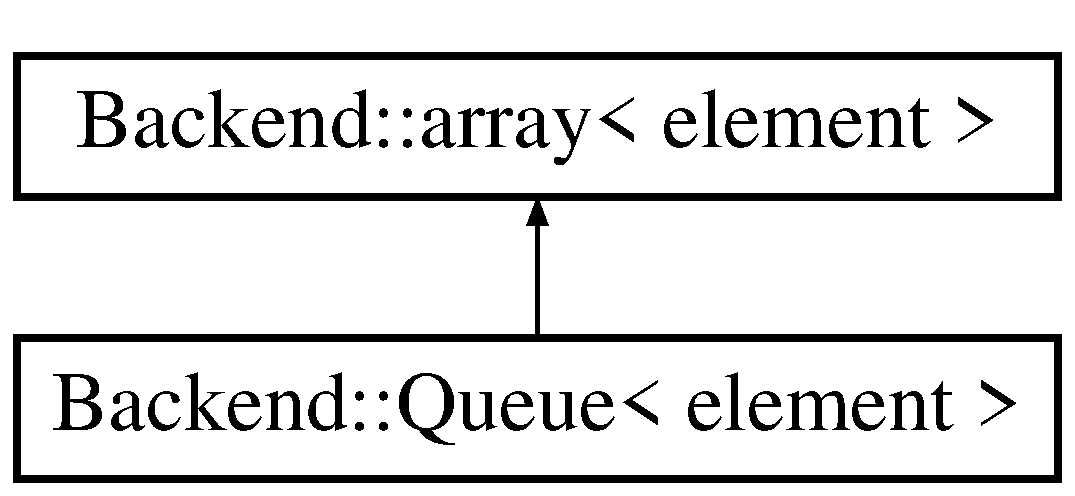
\includegraphics[height=2.000000cm]{classBackend_1_1array}
\end{center}
\end{figure}
\subsection*{Public Types}
\begin{DoxyCompactItemize}
\item 
typedef element $\ast$ \hyperlink{classBackend_1_1array_a6d8785dc8b979153ef122f4e3bad1408}{pointer}
\item 
typedef element \& \hyperlink{classBackend_1_1array_aa98075b8d7a4e63ea919ee9d1d4df4a9}{reference}
\end{DoxyCompactItemize}
\subsection*{Public Member Functions}
\begin{DoxyCompactItemize}
\item 
\hyperlink{classBackend_1_1array_a66b527d78881f22d8b8508492f255122}{array} ()
\item 
\hyperlink{classBackend_1_1array_aea145bb4183732b07f1ea2c5ef74406e}{array} (unsigned long size)
\item 
\hyperlink{classBackend_1_1array_ac15cb5df923a27aae58573b2a798a564}{array} (\hyperlink{classBackend_1_1array}{array}$<$ element $>$ const \&other)
\item 
\hyperlink{classBackend_1_1array}{array}$<$ element $>$ \& \hyperlink{classBackend_1_1array_abab978602a61af66f73e4951e5779554}{operator=} (\hyperlink{classBackend_1_1array}{array}$<$ element $>$ const \&other)
\item 
virtual \hyperlink{classBackend_1_1array_af036a9cb5baeb7acdda453ffc25e8b5f}{$\sim$array} ()
\item 
element \& \hyperlink{classBackend_1_1array_a906073a0b37d9abef728f2c188e73a5a}{operator\mbox{[}$\,$\mbox{]}} (unsigned long const \&index)
\item 
unsigned long const \& \hyperlink{classBackend_1_1array_a7b74d2da9eacbeea96b1661962a03970}{Size} () const 
\end{DoxyCompactItemize}
\subsection*{Protected Attributes}
\begin{DoxyCompactItemize}
\item 
element $\ast$ \hyperlink{classBackend_1_1array_ac588c1e30c2c4748bc9a5bb12b9320af}{\+\_\+array}
\item 
unsigned long \hyperlink{classBackend_1_1array_ae51d64e87b42931946111c28b98e8a18}{\+\_\+size}
\end{DoxyCompactItemize}


\subsection{Detailed Description}
\subsubsection*{template$<$class element$>$class Backend\+::array$<$ element $>$}



Definition at line 27 of file Queue.\+h.



\subsection{Member Typedef Documentation}
\hypertarget{classBackend_1_1array_a6d8785dc8b979153ef122f4e3bad1408}{\index{Backend\+::array@{Backend\+::array}!pointer@{pointer}}
\index{pointer@{pointer}!Backend\+::array@{Backend\+::array}}
\subsubsection[{pointer}]{\setlength{\rightskip}{0pt plus 5cm}template$<$class element$>$ typedef element$\ast$ {\bf Backend\+::array}$<$ element $>$\+::{\bf pointer}}}\label{classBackend_1_1array_a6d8785dc8b979153ef122f4e3bad1408}


Definition at line 29 of file Queue.\+h.

\hypertarget{classBackend_1_1array_aa98075b8d7a4e63ea919ee9d1d4df4a9}{\index{Backend\+::array@{Backend\+::array}!reference@{reference}}
\index{reference@{reference}!Backend\+::array@{Backend\+::array}}
\subsubsection[{reference}]{\setlength{\rightskip}{0pt plus 5cm}template$<$class element$>$ typedef element\& {\bf Backend\+::array}$<$ element $>$\+::{\bf reference}}}\label{classBackend_1_1array_aa98075b8d7a4e63ea919ee9d1d4df4a9}


Definition at line 30 of file Queue.\+h.



\subsection{Constructor \& Destructor Documentation}
\hypertarget{classBackend_1_1array_a66b527d78881f22d8b8508492f255122}{\index{Backend\+::array@{Backend\+::array}!array@{array}}
\index{array@{array}!Backend\+::array@{Backend\+::array}}
\subsubsection[{array}]{\setlength{\rightskip}{0pt plus 5cm}template$<$class element$>$ {\bf Backend\+::array}$<$ element $>$\+::{\bf array} (
\begin{DoxyParamCaption}
{}
\end{DoxyParamCaption}
)\hspace{0.3cm}{\ttfamily [inline]}}}\label{classBackend_1_1array_a66b527d78881f22d8b8508492f255122}


Definition at line 32 of file Queue.\+h.


\begin{DoxyCode}
32 :\hyperlink{classBackend_1_1array_ae51d64e87b42931946111c28b98e8a18}{\_size}(0),\hyperlink{classBackend_1_1array_ac588c1e30c2c4748bc9a5bb12b9320af}{\_array}(\textcolor{keyword}{nullptr})\{\}
\end{DoxyCode}
\hypertarget{classBackend_1_1array_aea145bb4183732b07f1ea2c5ef74406e}{\index{Backend\+::array@{Backend\+::array}!array@{array}}
\index{array@{array}!Backend\+::array@{Backend\+::array}}
\subsubsection[{array}]{\setlength{\rightskip}{0pt plus 5cm}template$<$class element$>$ {\bf Backend\+::array}$<$ element $>$\+::{\bf array} (
\begin{DoxyParamCaption}
\item[{unsigned long}]{size}
\end{DoxyParamCaption}
)\hspace{0.3cm}{\ttfamily [inline]}}}\label{classBackend_1_1array_aea145bb4183732b07f1ea2c5ef74406e}


Definition at line 33 of file Queue.\+h.


\begin{DoxyCode}
33 :\hyperlink{classBackend_1_1array_ae51d64e87b42931946111c28b98e8a18}{\_size}(size),\hyperlink{classBackend_1_1array_ac588c1e30c2c4748bc9a5bb12b9320af}{\_array}(\textcolor{keyword}{new} element[size])\{\}
\end{DoxyCode}
\hypertarget{classBackend_1_1array_ac15cb5df923a27aae58573b2a798a564}{\index{Backend\+::array@{Backend\+::array}!array@{array}}
\index{array@{array}!Backend\+::array@{Backend\+::array}}
\subsubsection[{array}]{\setlength{\rightskip}{0pt plus 5cm}template$<$class element$>$ {\bf Backend\+::array}$<$ element $>$\+::{\bf array} (
\begin{DoxyParamCaption}
\item[{{\bf array}$<$ element $>$ const \&}]{other}
\end{DoxyParamCaption}
)\hspace{0.3cm}{\ttfamily [inline]}}}\label{classBackend_1_1array_ac15cb5df923a27aae58573b2a798a564}


Definition at line 34 of file Queue.\+h.


\begin{DoxyCode}
34                                           \{
35             \hyperlink{classBackend_1_1array_ac588c1e30c2c4748bc9a5bb12b9320af}{\_array} = \textcolor{keyword}{new} element[other.Size()];
36             \hyperlink{classBackend_1_1array_ae51d64e87b42931946111c28b98e8a18}{\_size} = other.Size();
37             *\textcolor{keyword}{this} = other;
38         \}
\end{DoxyCode}
\hypertarget{classBackend_1_1array_af036a9cb5baeb7acdda453ffc25e8b5f}{\index{Backend\+::array@{Backend\+::array}!````~array@{$\sim$array}}
\index{````~array@{$\sim$array}!Backend\+::array@{Backend\+::array}}
\subsubsection[{$\sim$array}]{\setlength{\rightskip}{0pt plus 5cm}template$<$class element$>$ virtual {\bf Backend\+::array}$<$ element $>$\+::$\sim${\bf array} (
\begin{DoxyParamCaption}
{}
\end{DoxyParamCaption}
)\hspace{0.3cm}{\ttfamily [inline]}, {\ttfamily [virtual]}}}\label{classBackend_1_1array_af036a9cb5baeb7acdda453ffc25e8b5f}


Definition at line 52 of file Queue.\+h.


\begin{DoxyCode}
52                         \{
53             \textcolor{keywordflow}{if} (\hyperlink{classBackend_1_1array_ac588c1e30c2c4748bc9a5bb12b9320af}{\_array}!=\textcolor{keyword}{nullptr}) \{
54                 \textcolor{keyword}{delete} [] \hyperlink{classBackend_1_1array_ac588c1e30c2c4748bc9a5bb12b9320af}{\_array};
55             \}
56             \hyperlink{classBackend_1_1array_ae51d64e87b42931946111c28b98e8a18}{\_size}=0;
57         \}
\end{DoxyCode}


\subsection{Member Function Documentation}
\hypertarget{classBackend_1_1array_abab978602a61af66f73e4951e5779554}{\index{Backend\+::array@{Backend\+::array}!operator=@{operator=}}
\index{operator=@{operator=}!Backend\+::array@{Backend\+::array}}
\subsubsection[{operator=}]{\setlength{\rightskip}{0pt plus 5cm}template$<$class element$>$ {\bf array}$<$element$>$\& {\bf Backend\+::array}$<$ element $>$\+::operator= (
\begin{DoxyParamCaption}
\item[{{\bf array}$<$ element $>$ const \&}]{other}
\end{DoxyParamCaption}
)\hspace{0.3cm}{\ttfamily [inline]}}}\label{classBackend_1_1array_abab978602a61af66f73e4951e5779554}


Definition at line 39 of file Queue.\+h.


\begin{DoxyCode}
39                                                               \{
40             \textcolor{keywordflow}{if} (\hyperlink{classBackend_1_1array_ae51d64e87b42931946111c28b98e8a18}{\_size}!=other.\_size) \{
41                 \textcolor{keywordflow}{if} (\hyperlink{classBackend_1_1array_ac588c1e30c2c4748bc9a5bb12b9320af}{\_array}!=\textcolor{keyword}{nullptr}) \{
42                     \textcolor{keyword}{delete} [] \hyperlink{classBackend_1_1array_ac588c1e30c2c4748bc9a5bb12b9320af}{\_array};
43                 \}
44                 \hyperlink{classBackend_1_1array_ae51d64e87b42931946111c28b98e8a18}{\_size} = other.\_size;
45                 \hyperlink{classBackend_1_1array_ac588c1e30c2c4748bc9a5bb12b9320af}{\_array} = \textcolor{keyword}{new} element[\hyperlink{classBackend_1_1array_ae51d64e87b42931946111c28b98e8a18}{\_size}];
46             \}
47             \textcolor{keywordflow}{for} (\textcolor{keywordtype}{int} i=0; i<\hyperlink{classBackend_1_1array_ae51d64e87b42931946111c28b98e8a18}{\_size}; ++i) \{
48                 \hyperlink{classBackend_1_1array_ac588c1e30c2c4748bc9a5bb12b9320af}{\_array}[i] = other.\_array[i];
49             \}
50             \textcolor{keywordflow}{return} *\textcolor{keyword}{this};
51         \}
\end{DoxyCode}
\hypertarget{classBackend_1_1array_a906073a0b37d9abef728f2c188e73a5a}{\index{Backend\+::array@{Backend\+::array}!operator\mbox{[}$\,$\mbox{]}@{operator[]}}
\index{operator\mbox{[}$\,$\mbox{]}@{operator[]}!Backend\+::array@{Backend\+::array}}
\subsubsection[{operator[]}]{\setlength{\rightskip}{0pt plus 5cm}template$<$class element$>$ element\& {\bf Backend\+::array}$<$ element $>$\+::operator\mbox{[}$\,$\mbox{]} (
\begin{DoxyParamCaption}
\item[{unsigned long const \&}]{index}
\end{DoxyParamCaption}
)\hspace{0.3cm}{\ttfamily [inline]}}}\label{classBackend_1_1array_a906073a0b37d9abef728f2c188e73a5a}


Definition at line 58 of file Queue.\+h.


\begin{DoxyCode}
58                                                        \{
59 \textcolor{preprocessor}{#ifdef DEBUG}
60             assert(index<\hyperlink{classBackend_1_1array_ae51d64e87b42931946111c28b98e8a18}{\_size});
61 \textcolor{preprocessor}{#endif}
62             \textcolor{keywordflow}{return} \hyperlink{classBackend_1_1array_ac588c1e30c2c4748bc9a5bb12b9320af}{\_array}[index];
63         \}
\end{DoxyCode}
\hypertarget{classBackend_1_1array_a7b74d2da9eacbeea96b1661962a03970}{\index{Backend\+::array@{Backend\+::array}!Size@{Size}}
\index{Size@{Size}!Backend\+::array@{Backend\+::array}}
\subsubsection[{Size}]{\setlength{\rightskip}{0pt plus 5cm}template$<$class element$>$ unsigned long const\& {\bf Backend\+::array}$<$ element $>$\+::Size (
\begin{DoxyParamCaption}
{}
\end{DoxyParamCaption}
) const\hspace{0.3cm}{\ttfamily [inline]}}}\label{classBackend_1_1array_a7b74d2da9eacbeea96b1661962a03970}


Definition at line 64 of file Queue.\+h.


\begin{DoxyCode}
64                                         \{
65             \textcolor{keywordflow}{return} \hyperlink{classBackend_1_1array_ae51d64e87b42931946111c28b98e8a18}{\_size};
66         \}
\end{DoxyCode}


\subsection{Member Data Documentation}
\hypertarget{classBackend_1_1array_ac588c1e30c2c4748bc9a5bb12b9320af}{\index{Backend\+::array@{Backend\+::array}!\+\_\+array@{\+\_\+array}}
\index{\+\_\+array@{\+\_\+array}!Backend\+::array@{Backend\+::array}}
\subsubsection[{\+\_\+array}]{\setlength{\rightskip}{0pt plus 5cm}template$<$class element$>$ element$\ast$ {\bf Backend\+::array}$<$ element $>$\+::\+\_\+array\hspace{0.3cm}{\ttfamily [protected]}}}\label{classBackend_1_1array_ac588c1e30c2c4748bc9a5bb12b9320af}


Definition at line 68 of file Queue.\+h.

\hypertarget{classBackend_1_1array_ae51d64e87b42931946111c28b98e8a18}{\index{Backend\+::array@{Backend\+::array}!\+\_\+size@{\+\_\+size}}
\index{\+\_\+size@{\+\_\+size}!Backend\+::array@{Backend\+::array}}
\subsubsection[{\+\_\+size}]{\setlength{\rightskip}{0pt plus 5cm}template$<$class element$>$ unsigned long {\bf Backend\+::array}$<$ element $>$\+::\+\_\+size\hspace{0.3cm}{\ttfamily [protected]}}}\label{classBackend_1_1array_ae51d64e87b42931946111c28b98e8a18}


Definition at line 69 of file Queue.\+h.



The documentation for this class was generated from the following file\+:\begin{DoxyCompactItemize}
\item 
/\+Users/alexanderzywicki/\+Documents/\+School\+\_\+\+Stuff/\+Fall\+\_\+2014/\+Digital\+\_\+\+Signal\+\_\+\+Generation\+\_\+and\+\_\+\+Analysis/src/include/\hyperlink{Queue_8h}{Queue.\+h}\end{DoxyCompactItemize}

\hypertarget{classSignal_1_1BLIT_1_1BLIT}{\section{Signal\+:\+:B\+L\+I\+T\+:\+:B\+L\+I\+T Class Reference}
\label{classSignal_1_1BLIT_1_1BLIT}\index{Signal\+::\+B\+L\+I\+T\+::\+B\+L\+I\+T@{Signal\+::\+B\+L\+I\+T\+::\+B\+L\+I\+T}}
}


{\ttfamily \#include $<$B\+L\+I\+T.\+h$>$}

Inheritance diagram for Signal\+:\+:B\+L\+I\+T\+:\+:B\+L\+I\+T\+:\begin{figure}[H]
\begin{center}
\leavevmode
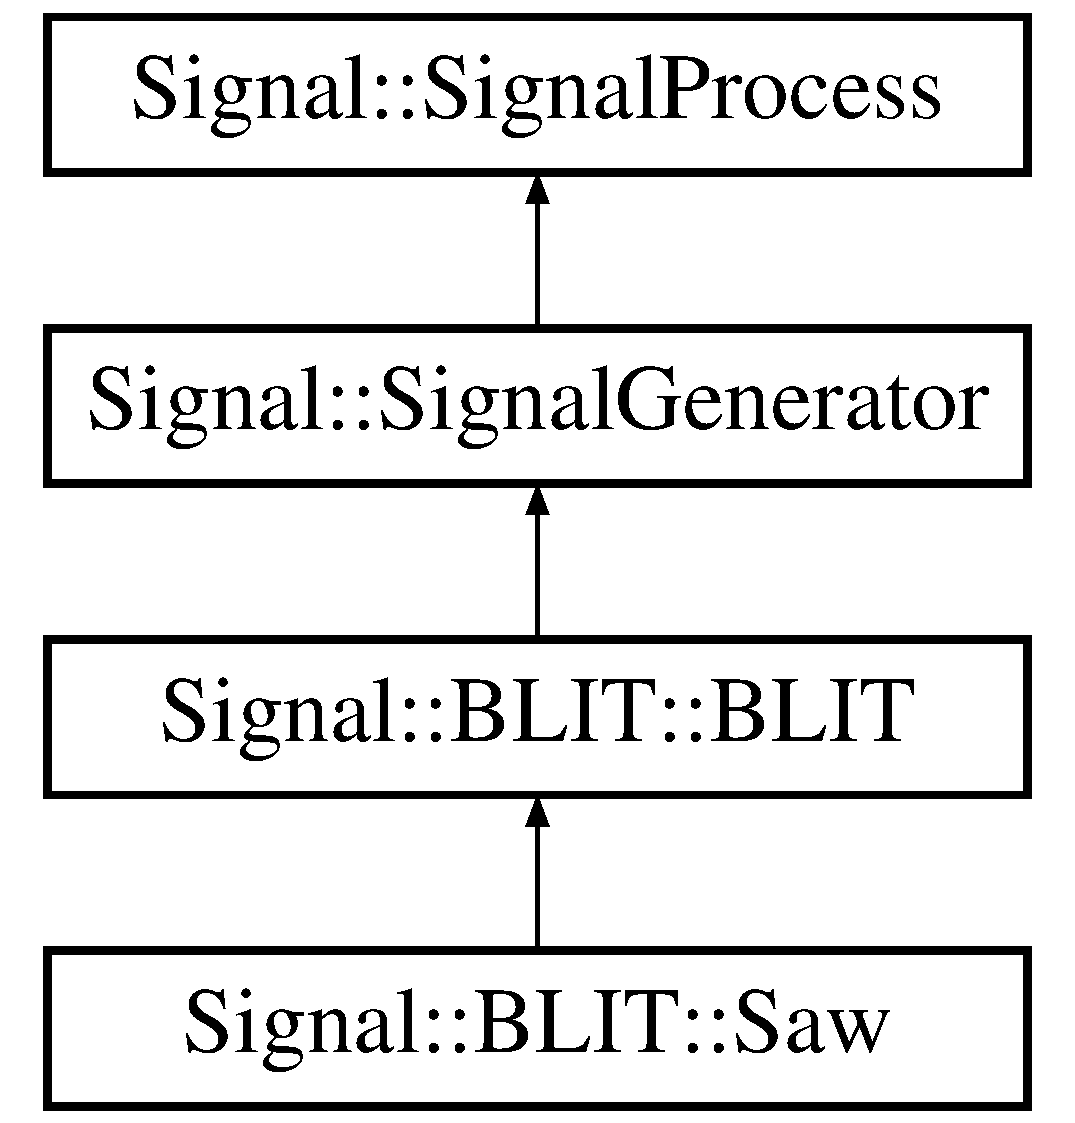
\includegraphics[height=4.000000cm]{classSignal_1_1BLIT_1_1BLIT}
\end{center}
\end{figure}
\subsection*{Public Member Functions}
\begin{DoxyCompactItemize}
\item 
\hyperlink{classSignal_1_1BLIT_1_1BLIT_ad22461c308981ee86ddc8b992bfbaf27}{B\+L\+I\+T} ()
\item 
\hyperlink{classSignal_1_1BLIT_1_1BLIT_af4f90ac6dfddc173dd0b381f6582dac9}{B\+L\+I\+T} (double const \&frequency, double const \&phase\+\_\+offset)
\item 
virtual \hyperlink{classSignal_1_1BLIT_1_1BLIT_a9355800dce797a6d35d8bbfc7eb9b834}{$\sim$\+B\+L\+I\+T} ()
\item 
virtual double const \& \hyperlink{classSignal_1_1BLIT_1_1BLIT_a59110620478308054d4c932c613e5cc6}{Frequency} (double const \&value)
\item 
virtual bool \hyperlink{classSignal_1_1BLIT_1_1BLIT_a98982b34bc6c9ca4c2e91550afa31375}{Perform} (\hyperlink{classSignal_1_1Sample}{Sample} \&signal)
\item 
virtual bool \hyperlink{classSignal_1_1BLIT_1_1BLIT_a2f0ee604ed0e67557aa9f7e7f50d80ec}{Perform} (\hyperlink{classSignal_1_1RingBuffer}{Ring\+Buffer} \&signal)
\item 
virtual double const \& \hyperlink{classSignal_1_1SignalGenerator_a96af42ee68f94e9b04d034fd68b73ecd}{Frequency} () const 
\item 
virtual double const \& \hyperlink{classSignal_1_1SignalGenerator_ac2538ec946f001e394d2416fda698d1c}{Phase\+Offset} () const 
\item 
virtual double const \& \hyperlink{classSignal_1_1SignalGenerator_ac6a103ff72beaa338f6d18c812522d78}{Phase\+Offset} (double const \&value)
\end{DoxyCompactItemize}
\subsection*{Protected Member Functions}
\begin{DoxyCompactItemize}
\item 
virtual void \hyperlink{classSignal_1_1BLIT_1_1BLIT_abec1466e0fe67fcdd52127ab34b7a3a4}{update\+Harms} ()
\item 
double \hyperlink{classSignal_1_1BLIT_1_1BLIT_ae552ae6350f291dd14198f88fbda0359}{\+\_\+pstep} ()
\item 
double \hyperlink{classSignal_1_1BLIT_1_1BLIT_a09820c226748516af14ff25043f1c51a}{\+\_\+pstep\+\_\+rad} ()
\item 
void \hyperlink{classSignal_1_1BLIT_1_1BLIT_ad0ede061ea6ca1db803d16ac8c968875}{\+\_\+psync} ()
\end{DoxyCompactItemize}
\subsection*{Protected Attributes}
\begin{DoxyCompactItemize}
\item 
\hyperlink{classSignal_1_1Sample}{Sample} \hyperlink{classSignal_1_1BLIT_1_1BLIT_ae3db6ee922897295fdf93a3b3c3dfadd}{\+\_\+sample}
\item 
unsigned long \hyperlink{classSignal_1_1BLIT_1_1BLIT_a0bfbf4e7515a42fab7df748b8497f648}{\+\_\+n\+Harms}
\item 
unsigned long \hyperlink{classSignal_1_1BLIT_1_1BLIT_a314aae37a0a53fa3f79a4466b9558fa5}{m\+\_\+}
\item 
double \hyperlink{classSignal_1_1BLIT_1_1BLIT_ae1ed1e1125cef25e6a0dfb8de3c296da}{\+\_\+phasor}
\item 
float \hyperlink{classSignal_1_1BLIT_1_1BLIT_afd06bf26696642f7eb400fb984e524f3}{phs}
\item 
float \hyperlink{classSignal_1_1BLIT_1_1BLIT_aa543d207e6dd260762652221c598bae9}{tmp}
\item 
float \hyperlink{classSignal_1_1BLIT_1_1BLIT_abef50d7ff7da92f5f0a8482287b47ae5}{\+\_\+denominator}
\item 
double \hyperlink{classSignal_1_1SignalGenerator_a7f107461333bce68c5dad412db96a8c2}{\+\_\+frequency}
\item 
double \hyperlink{classSignal_1_1SignalGenerator_a85a4702347352bab1c71e0a8df8437d6}{\+\_\+f\+Hertz}
\item 
double \hyperlink{classSignal_1_1SignalGenerator_a6b4444d46747c8517171edbbf4b5588f}{\+\_\+phase\+\_\+offset}
\end{DoxyCompactItemize}


\subsection{Detailed Description}


Definition at line 20 of file B\+L\+I\+T.\+h.



\subsection{Constructor \& Destructor Documentation}
\hypertarget{classSignal_1_1BLIT_1_1BLIT_ad22461c308981ee86ddc8b992bfbaf27}{\index{Signal\+::\+B\+L\+I\+T\+::\+B\+L\+I\+T@{Signal\+::\+B\+L\+I\+T\+::\+B\+L\+I\+T}!B\+L\+I\+T@{B\+L\+I\+T}}
\index{B\+L\+I\+T@{B\+L\+I\+T}!Signal\+::\+B\+L\+I\+T\+::\+B\+L\+I\+T@{Signal\+::\+B\+L\+I\+T\+::\+B\+L\+I\+T}}
\subsubsection[{B\+L\+I\+T}]{\setlength{\rightskip}{0pt plus 5cm}Signal\+::\+B\+L\+I\+T\+::\+B\+L\+I\+T\+::\+B\+L\+I\+T (
\begin{DoxyParamCaption}
{}
\end{DoxyParamCaption}
)}}\label{classSignal_1_1BLIT_1_1BLIT_ad22461c308981ee86ddc8b992bfbaf27}


Definition at line 11 of file B\+L\+I\+T.\+cpp.


\begin{DoxyCode}
11                     :\hyperlink{classSignal_1_1SignalGenerator_a8c67c754d86e0363445d7fd271855e1a}{SignalGenerator}()\{
12     \hyperlink{classSignal_1_1BLIT_1_1BLIT_abec1466e0fe67fcdd52127ab34b7a3a4}{updateHarms}();
13 \}
\end{DoxyCode}
\hypertarget{classSignal_1_1BLIT_1_1BLIT_af4f90ac6dfddc173dd0b381f6582dac9}{\index{Signal\+::\+B\+L\+I\+T\+::\+B\+L\+I\+T@{Signal\+::\+B\+L\+I\+T\+::\+B\+L\+I\+T}!B\+L\+I\+T@{B\+L\+I\+T}}
\index{B\+L\+I\+T@{B\+L\+I\+T}!Signal\+::\+B\+L\+I\+T\+::\+B\+L\+I\+T@{Signal\+::\+B\+L\+I\+T\+::\+B\+L\+I\+T}}
\subsubsection[{B\+L\+I\+T}]{\setlength{\rightskip}{0pt plus 5cm}Signal\+::\+B\+L\+I\+T\+::\+B\+L\+I\+T\+::\+B\+L\+I\+T (
\begin{DoxyParamCaption}
\item[{double const \&}]{frequency, }
\item[{double const \&}]{phase\+\_\+offset}
\end{DoxyParamCaption}
)}}\label{classSignal_1_1BLIT_1_1BLIT_af4f90ac6dfddc173dd0b381f6582dac9}


Definition at line 14 of file B\+L\+I\+T.\+cpp.


\begin{DoxyCode}
14                                                                       :
      \hyperlink{classSignal_1_1SignalGenerator_a8c67c754d86e0363445d7fd271855e1a}{SignalGenerator}(frequency,phase\_offset)\{
15     \hyperlink{classSignal_1_1BLIT_1_1BLIT_abec1466e0fe67fcdd52127ab34b7a3a4}{updateHarms}();
16 \}
\end{DoxyCode}
\hypertarget{classSignal_1_1BLIT_1_1BLIT_a9355800dce797a6d35d8bbfc7eb9b834}{\index{Signal\+::\+B\+L\+I\+T\+::\+B\+L\+I\+T@{Signal\+::\+B\+L\+I\+T\+::\+B\+L\+I\+T}!````~B\+L\+I\+T@{$\sim$\+B\+L\+I\+T}}
\index{````~B\+L\+I\+T@{$\sim$\+B\+L\+I\+T}!Signal\+::\+B\+L\+I\+T\+::\+B\+L\+I\+T@{Signal\+::\+B\+L\+I\+T\+::\+B\+L\+I\+T}}
\subsubsection[{$\sim$\+B\+L\+I\+T}]{\setlength{\rightskip}{0pt plus 5cm}Signal\+::\+B\+L\+I\+T\+::\+B\+L\+I\+T\+::$\sim$\+B\+L\+I\+T (
\begin{DoxyParamCaption}
{}
\end{DoxyParamCaption}
)\hspace{0.3cm}{\ttfamily [virtual]}}}\label{classSignal_1_1BLIT_1_1BLIT_a9355800dce797a6d35d8bbfc7eb9b834}


Definition at line 17 of file B\+L\+I\+T.\+cpp.


\begin{DoxyCode}
17 \{\}
\end{DoxyCode}


\subsection{Member Function Documentation}
\hypertarget{classSignal_1_1BLIT_1_1BLIT_ae552ae6350f291dd14198f88fbda0359}{\index{Signal\+::\+B\+L\+I\+T\+::\+B\+L\+I\+T@{Signal\+::\+B\+L\+I\+T\+::\+B\+L\+I\+T}!\+\_\+pstep@{\+\_\+pstep}}
\index{\+\_\+pstep@{\+\_\+pstep}!Signal\+::\+B\+L\+I\+T\+::\+B\+L\+I\+T@{Signal\+::\+B\+L\+I\+T\+::\+B\+L\+I\+T}}
\subsubsection[{\+\_\+pstep}]{\setlength{\rightskip}{0pt plus 5cm}double Signal\+::\+B\+L\+I\+T\+::\+B\+L\+I\+T\+::\+\_\+pstep (
\begin{DoxyParamCaption}
{}
\end{DoxyParamCaption}
)\hspace{0.3cm}{\ttfamily [inline]}, {\ttfamily [protected]}}}\label{classSignal_1_1BLIT_1_1BLIT_ae552ae6350f291dd14198f88fbda0359}


Definition at line 75 of file B\+L\+I\+T.\+h.


\begin{DoxyCode}
75                                   \{
76             \textcolor{keywordtype}{double} value = \hyperlink{classSignal_1_1BLIT_1_1BLIT_ae1ed1e1125cef25e6a0dfb8de3c296da}{\_phasor};
77             \hyperlink{classSignal_1_1BLIT_1_1BLIT_ae1ed1e1125cef25e6a0dfb8de3c296da}{\_phasor}+=\hyperlink{classSignal_1_1SignalGenerator_a7f107461333bce68c5dad412db96a8c2}{\_frequency};
78             \hyperlink{classSignal_1_1BLIT_1_1BLIT_ae1ed1e1125cef25e6a0dfb8de3c296da}{\_phasor} = \hyperlink{classSignal_1_1BLIT_1_1BLIT_ae1ed1e1125cef25e6a0dfb8de3c296da}{\_phasor}-(\textcolor{keywordtype}{unsigned} long)\hyperlink{classSignal_1_1BLIT_1_1BLIT_ae1ed1e1125cef25e6a0dfb8de3c296da}{\_phasor};\textcolor{comment}{//cheaper %1}
79             \textcolor{keywordflow}{return} value;
80         \}
\end{DoxyCode}
\hypertarget{classSignal_1_1BLIT_1_1BLIT_a09820c226748516af14ff25043f1c51a}{\index{Signal\+::\+B\+L\+I\+T\+::\+B\+L\+I\+T@{Signal\+::\+B\+L\+I\+T\+::\+B\+L\+I\+T}!\+\_\+pstep\+\_\+rad@{\+\_\+pstep\+\_\+rad}}
\index{\+\_\+pstep\+\_\+rad@{\+\_\+pstep\+\_\+rad}!Signal\+::\+B\+L\+I\+T\+::\+B\+L\+I\+T@{Signal\+::\+B\+L\+I\+T\+::\+B\+L\+I\+T}}
\subsubsection[{\+\_\+pstep\+\_\+rad}]{\setlength{\rightskip}{0pt plus 5cm}double Signal\+::\+B\+L\+I\+T\+::\+B\+L\+I\+T\+::\+\_\+pstep\+\_\+rad (
\begin{DoxyParamCaption}
{}
\end{DoxyParamCaption}
)\hspace{0.3cm}{\ttfamily [inline]}, {\ttfamily [protected]}}}\label{classSignal_1_1BLIT_1_1BLIT_a09820c226748516af14ff25043f1c51a}


Definition at line 81 of file B\+L\+I\+T.\+h.


\begin{DoxyCode}
81                                       \{
82             \textcolor{keywordflow}{return} \hyperlink{PI_8h_a4912c64aec0c943b7985db6cb61ff83a}{TWOPI} * \hyperlink{classSignal_1_1BLIT_1_1BLIT_ae552ae6350f291dd14198f88fbda0359}{\_pstep}();
83         \}
\end{DoxyCode}
\hypertarget{classSignal_1_1BLIT_1_1BLIT_ad0ede061ea6ca1db803d16ac8c968875}{\index{Signal\+::\+B\+L\+I\+T\+::\+B\+L\+I\+T@{Signal\+::\+B\+L\+I\+T\+::\+B\+L\+I\+T}!\+\_\+psync@{\+\_\+psync}}
\index{\+\_\+psync@{\+\_\+psync}!Signal\+::\+B\+L\+I\+T\+::\+B\+L\+I\+T@{Signal\+::\+B\+L\+I\+T\+::\+B\+L\+I\+T}}
\subsubsection[{\+\_\+psync}]{\setlength{\rightskip}{0pt plus 5cm}void Signal\+::\+B\+L\+I\+T\+::\+B\+L\+I\+T\+::\+\_\+psync (
\begin{DoxyParamCaption}
{}
\end{DoxyParamCaption}
)\hspace{0.3cm}{\ttfamily [inline]}, {\ttfamily [protected]}}}\label{classSignal_1_1BLIT_1_1BLIT_ad0ede061ea6ca1db803d16ac8c968875}


Definition at line 84 of file B\+L\+I\+T.\+h.


\begin{DoxyCode}
84                                 \{
85             \hyperlink{classSignal_1_1BLIT_1_1BLIT_ae1ed1e1125cef25e6a0dfb8de3c296da}{\_phasor} = 0;
86         \}
\end{DoxyCode}
\hypertarget{classSignal_1_1BLIT_1_1BLIT_a59110620478308054d4c932c613e5cc6}{\index{Signal\+::\+B\+L\+I\+T\+::\+B\+L\+I\+T@{Signal\+::\+B\+L\+I\+T\+::\+B\+L\+I\+T}!Frequency@{Frequency}}
\index{Frequency@{Frequency}!Signal\+::\+B\+L\+I\+T\+::\+B\+L\+I\+T@{Signal\+::\+B\+L\+I\+T\+::\+B\+L\+I\+T}}
\subsubsection[{Frequency}]{\setlength{\rightskip}{0pt plus 5cm}double const \& Signal\+::\+B\+L\+I\+T\+::\+B\+L\+I\+T\+::\+Frequency (
\begin{DoxyParamCaption}
\item[{double const \&}]{value}
\end{DoxyParamCaption}
)\hspace{0.3cm}{\ttfamily [virtual]}}}\label{classSignal_1_1BLIT_1_1BLIT_a59110620478308054d4c932c613e5cc6}


Reimplemented from \hyperlink{classSignal_1_1SignalGenerator_af83b532bf3ddc3637c2fd7a1dfd095cb}{Signal\+::\+Signal\+Generator}.



Definition at line 19 of file B\+L\+I\+T.\+cpp.


\begin{DoxyCode}
19                                                           \{
20     this->\hyperlink{classSignal_1_1SignalGenerator_a96af42ee68f94e9b04d034fd68b73ecd}{SignalGenerator::Frequency}(value);
21     \hyperlink{classSignal_1_1BLIT_1_1BLIT_abec1466e0fe67fcdd52127ab34b7a3a4}{updateHarms}();
22     \textcolor{keywordflow}{return} this->\hyperlink{classSignal_1_1SignalGenerator_a85a4702347352bab1c71e0a8df8437d6}{\_fHertz};
23 \}
\end{DoxyCode}
\hypertarget{classSignal_1_1SignalGenerator_a96af42ee68f94e9b04d034fd68b73ecd}{\index{Signal\+::\+B\+L\+I\+T\+::\+B\+L\+I\+T@{Signal\+::\+B\+L\+I\+T\+::\+B\+L\+I\+T}!Frequency@{Frequency}}
\index{Frequency@{Frequency}!Signal\+::\+B\+L\+I\+T\+::\+B\+L\+I\+T@{Signal\+::\+B\+L\+I\+T\+::\+B\+L\+I\+T}}
\subsubsection[{Frequency}]{\setlength{\rightskip}{0pt plus 5cm}double const \& Signal\+::\+Signal\+Generator\+::\+Frequency (
\begin{DoxyParamCaption}
{}
\end{DoxyParamCaption}
) const\hspace{0.3cm}{\ttfamily [virtual]}, {\ttfamily [inherited]}}}\label{classSignal_1_1SignalGenerator_a96af42ee68f94e9b04d034fd68b73ecd}


Definition at line 16 of file Signal\+Generator.\+cpp.


\begin{DoxyCode}
16                                                    \{
17     \textcolor{keywordflow}{return} \hyperlink{classSignal_1_1SignalGenerator_a85a4702347352bab1c71e0a8df8437d6}{\_fHertz};
18 \}
\end{DoxyCode}
\hypertarget{classSignal_1_1BLIT_1_1BLIT_a98982b34bc6c9ca4c2e91550afa31375}{\index{Signal\+::\+B\+L\+I\+T\+::\+B\+L\+I\+T@{Signal\+::\+B\+L\+I\+T\+::\+B\+L\+I\+T}!Perform@{Perform}}
\index{Perform@{Perform}!Signal\+::\+B\+L\+I\+T\+::\+B\+L\+I\+T@{Signal\+::\+B\+L\+I\+T\+::\+B\+L\+I\+T}}
\subsubsection[{Perform}]{\setlength{\rightskip}{0pt plus 5cm}bool Signal\+::\+B\+L\+I\+T\+::\+B\+L\+I\+T\+::\+Perform (
\begin{DoxyParamCaption}
\item[{{\bf Sample} \&}]{signal}
\end{DoxyParamCaption}
)\hspace{0.3cm}{\ttfamily [inline]}, {\ttfamily [virtual]}}}\label{classSignal_1_1BLIT_1_1BLIT_a98982b34bc6c9ca4c2e91550afa31375}


Reimplemented from \hyperlink{classSignal_1_1SignalGenerator_a2cd9061c5ae40a392a9476551b4379f3}{Signal\+::\+Signal\+Generator}.



Definition at line 53 of file B\+L\+I\+T.\+h.


\begin{DoxyCode}
53                                                \{
54             \hyperlink{classSignal_1_1BLIT_1_1BLIT_afd06bf26696642f7eb400fb984e524f3}{phs} =\hyperlink{namespaceBackend_1_1Taylor_afda165e6dde636dd0f7b32031a71c7df}{Backend::Taylor::Sine}(\hyperlink{classSignal_1_1BLIT_1_1BLIT_a09820c226748516af14ff25043f1c51a}{\_pstep\_rad}());
55             \hyperlink{classSignal_1_1BLIT_1_1BLIT_abef50d7ff7da92f5f0a8482287b47ae5}{\_denominator} = \hyperlink{classSignal_1_1BLIT_1_1BLIT_afd06bf26696642f7eb400fb984e524f3}{phs};
56             \textcolor{keywordflow}{if} (\hyperlink{classSignal_1_1BLIT_1_1BLIT_abef50d7ff7da92f5f0a8482287b47ae5}{\_denominator}<=std::numeric\_limits<float>::epsilon()) \{
57                 \hyperlink{classSignal_1_1BLIT_1_1BLIT_aa543d207e6dd260762652221c598bae9}{tmp}=1.0;
58             \}\textcolor{keywordflow}{else}\{
59                 \hyperlink{classSignal_1_1BLIT_1_1BLIT_aa543d207e6dd260762652221c598bae9}{tmp} = \hyperlink{namespaceBackend_1_1Taylor_afda165e6dde636dd0f7b32031a71c7df}{Backend::Taylor::Sine}(\hyperlink{classSignal_1_1BLIT_1_1BLIT_afd06bf26696642f7eb400fb984e524f3}{phs}*\hyperlink{classSignal_1_1BLIT_1_1BLIT_a314aae37a0a53fa3f79a4466b9558fa5}{m\_});
60                 \hyperlink{classSignal_1_1BLIT_1_1BLIT_aa543d207e6dd260762652221c598bae9}{tmp}/= \hyperlink{classSignal_1_1BLIT_1_1BLIT_a314aae37a0a53fa3f79a4466b9558fa5}{m\_}* \hyperlink{classSignal_1_1BLIT_1_1BLIT_abef50d7ff7da92f5f0a8482287b47ae5}{\_denominator};
61             \}
62             signal = \hyperlink{classSignal_1_1BLIT_1_1BLIT_aa543d207e6dd260762652221c598bae9}{tmp};
63             \textcolor{keywordflow}{return} \textcolor{keyword}{true};
64         \}
\end{DoxyCode}
\hypertarget{classSignal_1_1BLIT_1_1BLIT_a2f0ee604ed0e67557aa9f7e7f50d80ec}{\index{Signal\+::\+B\+L\+I\+T\+::\+B\+L\+I\+T@{Signal\+::\+B\+L\+I\+T\+::\+B\+L\+I\+T}!Perform@{Perform}}
\index{Perform@{Perform}!Signal\+::\+B\+L\+I\+T\+::\+B\+L\+I\+T@{Signal\+::\+B\+L\+I\+T\+::\+B\+L\+I\+T}}
\subsubsection[{Perform}]{\setlength{\rightskip}{0pt plus 5cm}bool Signal\+::\+B\+L\+I\+T\+::\+B\+L\+I\+T\+::\+Perform (
\begin{DoxyParamCaption}
\item[{{\bf Ring\+Buffer} \&}]{signal}
\end{DoxyParamCaption}
)\hspace{0.3cm}{\ttfamily [inline]}, {\ttfamily [virtual]}}}\label{classSignal_1_1BLIT_1_1BLIT_a2f0ee604ed0e67557aa9f7e7f50d80ec}


Reimplemented from \hyperlink{classSignal_1_1SignalGenerator_a126d52dd9b6b14d33efc624e2c89284e}{Signal\+::\+Signal\+Generator}.



Definition at line 65 of file B\+L\+I\+T.\+h.


\begin{DoxyCode}
65                                                    \{
66             signal.Flush();
67             \textcolor{keywordflow}{while} (!signal.Full()) \{
68                 \textcolor{keywordflow}{if} (\hyperlink{classSignal_1_1BLIT_1_1BLIT_a98982b34bc6c9ca4c2e91550afa31375}{Perform}(\hyperlink{classSignal_1_1BLIT_1_1BLIT_ae3db6ee922897295fdf93a3b3c3dfadd}{\_sample})) \{
69                     \textcolor{keywordflow}{if}(signal.Write(\hyperlink{classSignal_1_1BLIT_1_1BLIT_ae3db6ee922897295fdf93a3b3c3dfadd}{\_sample}))\{
70                     \}\textcolor{keywordflow}{else} \textcolor{keywordflow}{return} \textcolor{keyword}{false};
71                 \}\textcolor{keywordflow}{else} \textcolor{keywordflow}{return} \textcolor{keyword}{false};
72             \}\textcolor{keywordflow}{return} \textcolor{keyword}{true};
73         \}
\end{DoxyCode}
\hypertarget{classSignal_1_1SignalGenerator_ac2538ec946f001e394d2416fda698d1c}{\index{Signal\+::\+B\+L\+I\+T\+::\+B\+L\+I\+T@{Signal\+::\+B\+L\+I\+T\+::\+B\+L\+I\+T}!Phase\+Offset@{Phase\+Offset}}
\index{Phase\+Offset@{Phase\+Offset}!Signal\+::\+B\+L\+I\+T\+::\+B\+L\+I\+T@{Signal\+::\+B\+L\+I\+T\+::\+B\+L\+I\+T}}
\subsubsection[{Phase\+Offset}]{\setlength{\rightskip}{0pt plus 5cm}double const \& Signal\+::\+Signal\+Generator\+::\+Phase\+Offset (
\begin{DoxyParamCaption}
{}
\end{DoxyParamCaption}
) const\hspace{0.3cm}{\ttfamily [virtual]}, {\ttfamily [inherited]}}}\label{classSignal_1_1SignalGenerator_ac2538ec946f001e394d2416fda698d1c}


Definition at line 24 of file Signal\+Generator.\+cpp.


\begin{DoxyCode}
24                                                      \{
25     \textcolor{keywordflow}{return} \hyperlink{classSignal_1_1SignalGenerator_a6b4444d46747c8517171edbbf4b5588f}{\_phase\_offset};
26 \}
\end{DoxyCode}
\hypertarget{classSignal_1_1SignalGenerator_ac6a103ff72beaa338f6d18c812522d78}{\index{Signal\+::\+B\+L\+I\+T\+::\+B\+L\+I\+T@{Signal\+::\+B\+L\+I\+T\+::\+B\+L\+I\+T}!Phase\+Offset@{Phase\+Offset}}
\index{Phase\+Offset@{Phase\+Offset}!Signal\+::\+B\+L\+I\+T\+::\+B\+L\+I\+T@{Signal\+::\+B\+L\+I\+T\+::\+B\+L\+I\+T}}
\subsubsection[{Phase\+Offset}]{\setlength{\rightskip}{0pt plus 5cm}double const \& Signal\+::\+Signal\+Generator\+::\+Phase\+Offset (
\begin{DoxyParamCaption}
\item[{double const \&}]{value}
\end{DoxyParamCaption}
)\hspace{0.3cm}{\ttfamily [virtual]}, {\ttfamily [inherited]}}}\label{classSignal_1_1SignalGenerator_ac6a103ff72beaa338f6d18c812522d78}


Definition at line 27 of file Signal\+Generator.\+cpp.


\begin{DoxyCode}
27                                                                    \{
28     \hyperlink{classSignal_1_1SignalGenerator_a6b4444d46747c8517171edbbf4b5588f}{\_phase\_offset} = value;
29     \textcolor{keywordflow}{return} \hyperlink{classSignal_1_1SignalGenerator_a6b4444d46747c8517171edbbf4b5588f}{\_phase\_offset};
30 \}
\end{DoxyCode}
\hypertarget{classSignal_1_1BLIT_1_1BLIT_abec1466e0fe67fcdd52127ab34b7a3a4}{\index{Signal\+::\+B\+L\+I\+T\+::\+B\+L\+I\+T@{Signal\+::\+B\+L\+I\+T\+::\+B\+L\+I\+T}!update\+Harms@{update\+Harms}}
\index{update\+Harms@{update\+Harms}!Signal\+::\+B\+L\+I\+T\+::\+B\+L\+I\+T@{Signal\+::\+B\+L\+I\+T\+::\+B\+L\+I\+T}}
\subsubsection[{update\+Harms}]{\setlength{\rightskip}{0pt plus 5cm}void Signal\+::\+B\+L\+I\+T\+::\+B\+L\+I\+T\+::update\+Harms (
\begin{DoxyParamCaption}
{}
\end{DoxyParamCaption}
)\hspace{0.3cm}{\ttfamily [protected]}, {\ttfamily [virtual]}}}\label{classSignal_1_1BLIT_1_1BLIT_abec1466e0fe67fcdd52127ab34b7a3a4}


Reimplemented in \hyperlink{classSignal_1_1BLIT_1_1BLITSaw_a9c8ad70fca571cc707eaa99649d74afc}{Signal\+::\+B\+L\+I\+T\+::\+B\+L\+I\+T\+Saw}.



Definition at line 24 of file B\+L\+I\+T.\+cpp.


\begin{DoxyCode}
24                                 \{
25     \textcolor{keywordflow}{if} (\hyperlink{classSignal_1_1BLIT_1_1BLIT_a0bfbf4e7515a42fab7df748b8497f648}{\_nHarms}<=0) \{
26         \textcolor{keywordtype}{size\_t} max = (size\_t)floor(0.5 * (\hyperlink{namespaceSignal_ae7b1f222afc010e0f33f306f978fcde9}{Sample\_Rate}()/ \hyperlink{classSignal_1_1SignalGenerator_a85a4702347352bab1c71e0a8df8437d6}{\_fHertz}));
27         \hyperlink{classSignal_1_1BLIT_1_1BLIT_a314aae37a0a53fa3f79a4466b9558fa5}{m\_} = 2* max +1;
28     \}
29     \textcolor{keywordflow}{else}\{
30         \hyperlink{classSignal_1_1BLIT_1_1BLIT_a314aae37a0a53fa3f79a4466b9558fa5}{m\_} = 2* \hyperlink{classSignal_1_1BLIT_1_1BLIT_a0bfbf4e7515a42fab7df748b8497f648}{\_nHarms} +1;
31     \}
32 \}\end{DoxyCode}


\subsection{Member Data Documentation}
\hypertarget{classSignal_1_1BLIT_1_1BLIT_abef50d7ff7da92f5f0a8482287b47ae5}{\index{Signal\+::\+B\+L\+I\+T\+::\+B\+L\+I\+T@{Signal\+::\+B\+L\+I\+T\+::\+B\+L\+I\+T}!\+\_\+denominator@{\+\_\+denominator}}
\index{\+\_\+denominator@{\+\_\+denominator}!Signal\+::\+B\+L\+I\+T\+::\+B\+L\+I\+T@{Signal\+::\+B\+L\+I\+T\+::\+B\+L\+I\+T}}
\subsubsection[{\+\_\+denominator}]{\setlength{\rightskip}{0pt plus 5cm}float Signal\+::\+B\+L\+I\+T\+::\+B\+L\+I\+T\+::\+\_\+denominator\hspace{0.3cm}{\ttfamily [protected]}}}\label{classSignal_1_1BLIT_1_1BLIT_abef50d7ff7da92f5f0a8482287b47ae5}


Definition at line 48 of file B\+L\+I\+T.\+h.

\hypertarget{classSignal_1_1SignalGenerator_a85a4702347352bab1c71e0a8df8437d6}{\index{Signal\+::\+B\+L\+I\+T\+::\+B\+L\+I\+T@{Signal\+::\+B\+L\+I\+T\+::\+B\+L\+I\+T}!\+\_\+f\+Hertz@{\+\_\+f\+Hertz}}
\index{\+\_\+f\+Hertz@{\+\_\+f\+Hertz}!Signal\+::\+B\+L\+I\+T\+::\+B\+L\+I\+T@{Signal\+::\+B\+L\+I\+T\+::\+B\+L\+I\+T}}
\subsubsection[{\+\_\+f\+Hertz}]{\setlength{\rightskip}{0pt plus 5cm}double Signal\+::\+Signal\+Generator\+::\+\_\+f\+Hertz\hspace{0.3cm}{\ttfamily [protected]}, {\ttfamily [inherited]}}}\label{classSignal_1_1SignalGenerator_a85a4702347352bab1c71e0a8df8437d6}


Definition at line 34 of file Signal\+Generator.\+h.

\hypertarget{classSignal_1_1SignalGenerator_a7f107461333bce68c5dad412db96a8c2}{\index{Signal\+::\+B\+L\+I\+T\+::\+B\+L\+I\+T@{Signal\+::\+B\+L\+I\+T\+::\+B\+L\+I\+T}!\+\_\+frequency@{\+\_\+frequency}}
\index{\+\_\+frequency@{\+\_\+frequency}!Signal\+::\+B\+L\+I\+T\+::\+B\+L\+I\+T@{Signal\+::\+B\+L\+I\+T\+::\+B\+L\+I\+T}}
\subsubsection[{\+\_\+frequency}]{\setlength{\rightskip}{0pt plus 5cm}double Signal\+::\+Signal\+Generator\+::\+\_\+frequency\hspace{0.3cm}{\ttfamily [protected]}, {\ttfamily [inherited]}}}\label{classSignal_1_1SignalGenerator_a7f107461333bce68c5dad412db96a8c2}


Definition at line 33 of file Signal\+Generator.\+h.

\hypertarget{classSignal_1_1BLIT_1_1BLIT_a0bfbf4e7515a42fab7df748b8497f648}{\index{Signal\+::\+B\+L\+I\+T\+::\+B\+L\+I\+T@{Signal\+::\+B\+L\+I\+T\+::\+B\+L\+I\+T}!\+\_\+n\+Harms@{\+\_\+n\+Harms}}
\index{\+\_\+n\+Harms@{\+\_\+n\+Harms}!Signal\+::\+B\+L\+I\+T\+::\+B\+L\+I\+T@{Signal\+::\+B\+L\+I\+T\+::\+B\+L\+I\+T}}
\subsubsection[{\+\_\+n\+Harms}]{\setlength{\rightskip}{0pt plus 5cm}unsigned long Signal\+::\+B\+L\+I\+T\+::\+B\+L\+I\+T\+::\+\_\+n\+Harms\hspace{0.3cm}{\ttfamily [protected]}}}\label{classSignal_1_1BLIT_1_1BLIT_a0bfbf4e7515a42fab7df748b8497f648}


Definition at line 32 of file B\+L\+I\+T.\+h.

\hypertarget{classSignal_1_1SignalGenerator_a6b4444d46747c8517171edbbf4b5588f}{\index{Signal\+::\+B\+L\+I\+T\+::\+B\+L\+I\+T@{Signal\+::\+B\+L\+I\+T\+::\+B\+L\+I\+T}!\+\_\+phase\+\_\+offset@{\+\_\+phase\+\_\+offset}}
\index{\+\_\+phase\+\_\+offset@{\+\_\+phase\+\_\+offset}!Signal\+::\+B\+L\+I\+T\+::\+B\+L\+I\+T@{Signal\+::\+B\+L\+I\+T\+::\+B\+L\+I\+T}}
\subsubsection[{\+\_\+phase\+\_\+offset}]{\setlength{\rightskip}{0pt plus 5cm}double Signal\+::\+Signal\+Generator\+::\+\_\+phase\+\_\+offset\hspace{0.3cm}{\ttfamily [protected]}, {\ttfamily [inherited]}}}\label{classSignal_1_1SignalGenerator_a6b4444d46747c8517171edbbf4b5588f}


Definition at line 35 of file Signal\+Generator.\+h.

\hypertarget{classSignal_1_1BLIT_1_1BLIT_ae1ed1e1125cef25e6a0dfb8de3c296da}{\index{Signal\+::\+B\+L\+I\+T\+::\+B\+L\+I\+T@{Signal\+::\+B\+L\+I\+T\+::\+B\+L\+I\+T}!\+\_\+phasor@{\+\_\+phasor}}
\index{\+\_\+phasor@{\+\_\+phasor}!Signal\+::\+B\+L\+I\+T\+::\+B\+L\+I\+T@{Signal\+::\+B\+L\+I\+T\+::\+B\+L\+I\+T}}
\subsubsection[{\+\_\+phasor}]{\setlength{\rightskip}{0pt plus 5cm}double Signal\+::\+B\+L\+I\+T\+::\+B\+L\+I\+T\+::\+\_\+phasor\hspace{0.3cm}{\ttfamily [protected]}}}\label{classSignal_1_1BLIT_1_1BLIT_ae1ed1e1125cef25e6a0dfb8de3c296da}


Definition at line 40 of file B\+L\+I\+T.\+h.

\hypertarget{classSignal_1_1BLIT_1_1BLIT_ae3db6ee922897295fdf93a3b3c3dfadd}{\index{Signal\+::\+B\+L\+I\+T\+::\+B\+L\+I\+T@{Signal\+::\+B\+L\+I\+T\+::\+B\+L\+I\+T}!\+\_\+sample@{\+\_\+sample}}
\index{\+\_\+sample@{\+\_\+sample}!Signal\+::\+B\+L\+I\+T\+::\+B\+L\+I\+T@{Signal\+::\+B\+L\+I\+T\+::\+B\+L\+I\+T}}
\subsubsection[{\+\_\+sample}]{\setlength{\rightskip}{0pt plus 5cm}{\bf Sample} Signal\+::\+B\+L\+I\+T\+::\+B\+L\+I\+T\+::\+\_\+sample\hspace{0.3cm}{\ttfamily [protected]}}}\label{classSignal_1_1BLIT_1_1BLIT_ae3db6ee922897295fdf93a3b3c3dfadd}


Definition at line 31 of file B\+L\+I\+T.\+h.

\hypertarget{classSignal_1_1BLIT_1_1BLIT_a314aae37a0a53fa3f79a4466b9558fa5}{\index{Signal\+::\+B\+L\+I\+T\+::\+B\+L\+I\+T@{Signal\+::\+B\+L\+I\+T\+::\+B\+L\+I\+T}!m\+\_\+@{m\+\_\+}}
\index{m\+\_\+@{m\+\_\+}!Signal\+::\+B\+L\+I\+T\+::\+B\+L\+I\+T@{Signal\+::\+B\+L\+I\+T\+::\+B\+L\+I\+T}}
\subsubsection[{m\+\_\+}]{\setlength{\rightskip}{0pt plus 5cm}unsigned long Signal\+::\+B\+L\+I\+T\+::\+B\+L\+I\+T\+::m\+\_\+\hspace{0.3cm}{\ttfamily [protected]}}}\label{classSignal_1_1BLIT_1_1BLIT_a314aae37a0a53fa3f79a4466b9558fa5}


Definition at line 33 of file B\+L\+I\+T.\+h.

\hypertarget{classSignal_1_1BLIT_1_1BLIT_afd06bf26696642f7eb400fb984e524f3}{\index{Signal\+::\+B\+L\+I\+T\+::\+B\+L\+I\+T@{Signal\+::\+B\+L\+I\+T\+::\+B\+L\+I\+T}!phs@{phs}}
\index{phs@{phs}!Signal\+::\+B\+L\+I\+T\+::\+B\+L\+I\+T@{Signal\+::\+B\+L\+I\+T\+::\+B\+L\+I\+T}}
\subsubsection[{phs}]{\setlength{\rightskip}{0pt plus 5cm}float Signal\+::\+B\+L\+I\+T\+::\+B\+L\+I\+T\+::phs\hspace{0.3cm}{\ttfamily [protected]}}}\label{classSignal_1_1BLIT_1_1BLIT_afd06bf26696642f7eb400fb984e524f3}


Definition at line 46 of file B\+L\+I\+T.\+h.

\hypertarget{classSignal_1_1BLIT_1_1BLIT_aa543d207e6dd260762652221c598bae9}{\index{Signal\+::\+B\+L\+I\+T\+::\+B\+L\+I\+T@{Signal\+::\+B\+L\+I\+T\+::\+B\+L\+I\+T}!tmp@{tmp}}
\index{tmp@{tmp}!Signal\+::\+B\+L\+I\+T\+::\+B\+L\+I\+T@{Signal\+::\+B\+L\+I\+T\+::\+B\+L\+I\+T}}
\subsubsection[{tmp}]{\setlength{\rightskip}{0pt plus 5cm}float Signal\+::\+B\+L\+I\+T\+::\+B\+L\+I\+T\+::tmp\hspace{0.3cm}{\ttfamily [protected]}}}\label{classSignal_1_1BLIT_1_1BLIT_aa543d207e6dd260762652221c598bae9}


Definition at line 47 of file B\+L\+I\+T.\+h.



The documentation for this class was generated from the following files\+:\begin{DoxyCompactItemize}
\item 
/\+Users/alexanderzywicki/\+Documents/\+School\+\_\+\+Stuff/\+Fall\+\_\+2014/\+Digital\+\_\+\+Signal\+\_\+\+Generation\+\_\+and\+\_\+\+Analysis/src/include/\hyperlink{BLIT_8h}{B\+L\+I\+T.\+h}\item 
/\+Users/alexanderzywicki/\+Documents/\+School\+\_\+\+Stuff/\+Fall\+\_\+2014/\+Digital\+\_\+\+Signal\+\_\+\+Generation\+\_\+and\+\_\+\+Analysis/src/\hyperlink{BLIT_8cpp}{B\+L\+I\+T.\+cpp}\end{DoxyCompactItemize}

\hypertarget{classSignal_1_1BLIT_1_1BLITSaw}{\section{Signal\+:\+:B\+L\+I\+T\+:\+:B\+L\+I\+T\+Saw Class Reference}
\label{classSignal_1_1BLIT_1_1BLITSaw}\index{Signal\+::\+B\+L\+I\+T\+::\+B\+L\+I\+T\+Saw@{Signal\+::\+B\+L\+I\+T\+::\+B\+L\+I\+T\+Saw}}
}


{\ttfamily \#include $<$B\+L\+I\+T\+Saw.\+h$>$}

Inheritance diagram for Signal\+:\+:B\+L\+I\+T\+:\+:B\+L\+I\+T\+Saw\+:\begin{figure}[H]
\begin{center}
\leavevmode
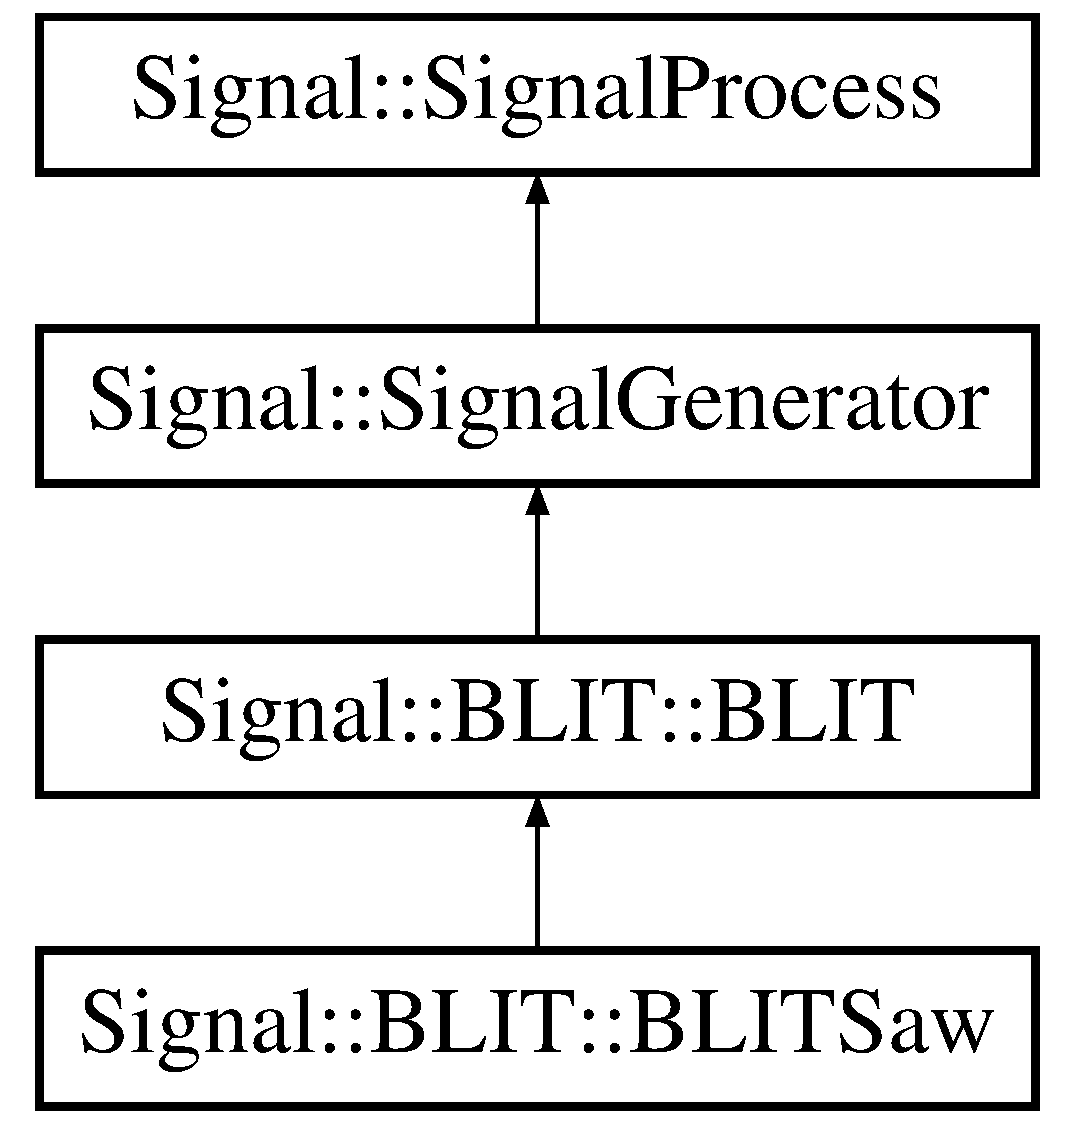
\includegraphics[height=4.000000cm]{classSignal_1_1BLIT_1_1BLITSaw}
\end{center}
\end{figure}
\subsection*{Public Member Functions}
\begin{DoxyCompactItemize}
\item 
virtual double const \& \hyperlink{classSignal_1_1SignalGenerator_a96af42ee68f94e9b04d034fd68b73ecd}{Frequency} () const 
\item 
virtual double const \& \hyperlink{classSignal_1_1SignalGenerator_ac2538ec946f001e394d2416fda698d1c}{Phase\+Offset} () const 
\item 
virtual double const \& \hyperlink{classSignal_1_1SignalGenerator_ac6a103ff72beaa338f6d18c812522d78}{Phase\+Offset} (double const \&value)
\end{DoxyCompactItemize}
\subsection*{Protected Member Functions}
\begin{DoxyCompactItemize}
\item 
virtual void \hyperlink{classSignal_1_1BLIT_1_1BLITSaw_a9c8ad70fca571cc707eaa99649d74afc}{update\+Harms} ()
\item 
double \hyperlink{classSignal_1_1BLIT_1_1BLIT_ae552ae6350f291dd14198f88fbda0359}{\+\_\+pstep} ()
\item 
double \hyperlink{classSignal_1_1BLIT_1_1BLIT_a09820c226748516af14ff25043f1c51a}{\+\_\+pstep\+\_\+rad} ()
\item 
void \hyperlink{classSignal_1_1BLIT_1_1BLIT_ad0ede061ea6ca1db803d16ac8c968875}{\+\_\+psync} ()
\end{DoxyCompactItemize}
\subsection*{Protected Attributes}
\begin{DoxyCompactItemize}
\item 
\hyperlink{classSignal_1_1Sample}{Sample} \hyperlink{classSignal_1_1BLIT_1_1BLIT_ae3db6ee922897295fdf93a3b3c3dfadd}{\+\_\+sample}
\item 
unsigned long \hyperlink{classSignal_1_1BLIT_1_1BLIT_a0bfbf4e7515a42fab7df748b8497f648}{\+\_\+n\+Harms}
\item 
unsigned long \hyperlink{classSignal_1_1BLIT_1_1BLIT_a314aae37a0a53fa3f79a4466b9558fa5}{m\+\_\+}
\item 
double \hyperlink{classSignal_1_1BLIT_1_1BLIT_ae1ed1e1125cef25e6a0dfb8de3c296da}{\+\_\+phasor}
\item 
float \hyperlink{classSignal_1_1BLIT_1_1BLIT_afd06bf26696642f7eb400fb984e524f3}{phs}
\item 
float \hyperlink{classSignal_1_1BLIT_1_1BLIT_aa543d207e6dd260762652221c598bae9}{tmp}
\item 
float \hyperlink{classSignal_1_1BLIT_1_1BLIT_abef50d7ff7da92f5f0a8482287b47ae5}{\+\_\+denominator}
\item 
double \hyperlink{classSignal_1_1SignalGenerator_a7f107461333bce68c5dad412db96a8c2}{\+\_\+frequency}
\item 
double \hyperlink{classSignal_1_1SignalGenerator_a85a4702347352bab1c71e0a8df8437d6}{\+\_\+f\+Hertz}
\item 
double \hyperlink{classSignal_1_1SignalGenerator_a6b4444d46747c8517171edbbf4b5588f}{\+\_\+phase\+\_\+offset}
\end{DoxyCompactItemize}


\subsection{Detailed Description}


Definition at line 18 of file B\+L\+I\+T\+Saw.\+h.



\subsection{Member Function Documentation}
\hypertarget{classSignal_1_1BLIT_1_1BLIT_ae552ae6350f291dd14198f88fbda0359}{\index{Signal\+::\+B\+L\+I\+T\+::\+B\+L\+I\+T\+Saw@{Signal\+::\+B\+L\+I\+T\+::\+B\+L\+I\+T\+Saw}!\+\_\+pstep@{\+\_\+pstep}}
\index{\+\_\+pstep@{\+\_\+pstep}!Signal\+::\+B\+L\+I\+T\+::\+B\+L\+I\+T\+Saw@{Signal\+::\+B\+L\+I\+T\+::\+B\+L\+I\+T\+Saw}}
\subsubsection[{\+\_\+pstep}]{\setlength{\rightskip}{0pt plus 5cm}double Signal\+::\+B\+L\+I\+T\+::\+B\+L\+I\+T\+::\+\_\+pstep (
\begin{DoxyParamCaption}
{}
\end{DoxyParamCaption}
)\hspace{0.3cm}{\ttfamily [inline]}, {\ttfamily [protected]}, {\ttfamily [inherited]}}}\label{classSignal_1_1BLIT_1_1BLIT_ae552ae6350f291dd14198f88fbda0359}


Definition at line 78 of file B\+L\+I\+T.\+h.


\begin{DoxyCode}
78                                   \{
79             \textcolor{keywordtype}{double} value = \hyperlink{classSignal_1_1BLIT_1_1BLIT_ae1ed1e1125cef25e6a0dfb8de3c296da}{\_phasor};
80             \hyperlink{classSignal_1_1BLIT_1_1BLIT_ae1ed1e1125cef25e6a0dfb8de3c296da}{\_phasor}+=\hyperlink{classSignal_1_1SignalGenerator_a7f107461333bce68c5dad412db96a8c2}{\_frequency};
81             \hyperlink{classSignal_1_1BLIT_1_1BLIT_ae1ed1e1125cef25e6a0dfb8de3c296da}{\_phasor} = \hyperlink{classSignal_1_1BLIT_1_1BLIT_ae1ed1e1125cef25e6a0dfb8de3c296da}{\_phasor}-(\textcolor{keywordtype}{unsigned} long)\hyperlink{classSignal_1_1BLIT_1_1BLIT_ae1ed1e1125cef25e6a0dfb8de3c296da}{\_phasor};\textcolor{comment}{//cheaper %1}
82             \textcolor{keywordflow}{return} value;
83         \}
\end{DoxyCode}
\hypertarget{classSignal_1_1BLIT_1_1BLIT_a09820c226748516af14ff25043f1c51a}{\index{Signal\+::\+B\+L\+I\+T\+::\+B\+L\+I\+T\+Saw@{Signal\+::\+B\+L\+I\+T\+::\+B\+L\+I\+T\+Saw}!\+\_\+pstep\+\_\+rad@{\+\_\+pstep\+\_\+rad}}
\index{\+\_\+pstep\+\_\+rad@{\+\_\+pstep\+\_\+rad}!Signal\+::\+B\+L\+I\+T\+::\+B\+L\+I\+T\+Saw@{Signal\+::\+B\+L\+I\+T\+::\+B\+L\+I\+T\+Saw}}
\subsubsection[{\+\_\+pstep\+\_\+rad}]{\setlength{\rightskip}{0pt plus 5cm}double Signal\+::\+B\+L\+I\+T\+::\+B\+L\+I\+T\+::\+\_\+pstep\+\_\+rad (
\begin{DoxyParamCaption}
{}
\end{DoxyParamCaption}
)\hspace{0.3cm}{\ttfamily [inline]}, {\ttfamily [protected]}, {\ttfamily [inherited]}}}\label{classSignal_1_1BLIT_1_1BLIT_a09820c226748516af14ff25043f1c51a}


Definition at line 84 of file B\+L\+I\+T.\+h.


\begin{DoxyCode}
84                                       \{
85             \textcolor{keywordflow}{return} \hyperlink{PI_8h_a4912c64aec0c943b7985db6cb61ff83a}{TWOPI} * \hyperlink{classSignal_1_1BLIT_1_1BLIT_ae552ae6350f291dd14198f88fbda0359}{\_pstep}();
86         \}
\end{DoxyCode}
\hypertarget{classSignal_1_1BLIT_1_1BLIT_ad0ede061ea6ca1db803d16ac8c968875}{\index{Signal\+::\+B\+L\+I\+T\+::\+B\+L\+I\+T\+Saw@{Signal\+::\+B\+L\+I\+T\+::\+B\+L\+I\+T\+Saw}!\+\_\+psync@{\+\_\+psync}}
\index{\+\_\+psync@{\+\_\+psync}!Signal\+::\+B\+L\+I\+T\+::\+B\+L\+I\+T\+Saw@{Signal\+::\+B\+L\+I\+T\+::\+B\+L\+I\+T\+Saw}}
\subsubsection[{\+\_\+psync}]{\setlength{\rightskip}{0pt plus 5cm}void Signal\+::\+B\+L\+I\+T\+::\+B\+L\+I\+T\+::\+\_\+psync (
\begin{DoxyParamCaption}
{}
\end{DoxyParamCaption}
)\hspace{0.3cm}{\ttfamily [inline]}, {\ttfamily [protected]}, {\ttfamily [inherited]}}}\label{classSignal_1_1BLIT_1_1BLIT_ad0ede061ea6ca1db803d16ac8c968875}


Definition at line 87 of file B\+L\+I\+T.\+h.


\begin{DoxyCode}
87                                 \{
88             \hyperlink{classSignal_1_1BLIT_1_1BLIT_ae1ed1e1125cef25e6a0dfb8de3c296da}{\_phasor} = 0;
89         \}
\end{DoxyCode}
\hypertarget{classSignal_1_1SignalGenerator_a96af42ee68f94e9b04d034fd68b73ecd}{\index{Signal\+::\+B\+L\+I\+T\+::\+B\+L\+I\+T\+Saw@{Signal\+::\+B\+L\+I\+T\+::\+B\+L\+I\+T\+Saw}!Frequency@{Frequency}}
\index{Frequency@{Frequency}!Signal\+::\+B\+L\+I\+T\+::\+B\+L\+I\+T\+Saw@{Signal\+::\+B\+L\+I\+T\+::\+B\+L\+I\+T\+Saw}}
\subsubsection[{Frequency}]{\setlength{\rightskip}{0pt plus 5cm}double const \& Signal\+::\+Signal\+Generator\+::\+Frequency (
\begin{DoxyParamCaption}
{}
\end{DoxyParamCaption}
) const\hspace{0.3cm}{\ttfamily [virtual]}, {\ttfamily [inherited]}}}\label{classSignal_1_1SignalGenerator_a96af42ee68f94e9b04d034fd68b73ecd}


Definition at line 16 of file Signal\+Generator.\+cpp.


\begin{DoxyCode}
16                                                    \{
17     \textcolor{keywordflow}{return} \hyperlink{classSignal_1_1SignalGenerator_a85a4702347352bab1c71e0a8df8437d6}{\_fHertz};
18 \}
\end{DoxyCode}
\hypertarget{classSignal_1_1SignalGenerator_ac2538ec946f001e394d2416fda698d1c}{\index{Signal\+::\+B\+L\+I\+T\+::\+B\+L\+I\+T\+Saw@{Signal\+::\+B\+L\+I\+T\+::\+B\+L\+I\+T\+Saw}!Phase\+Offset@{Phase\+Offset}}
\index{Phase\+Offset@{Phase\+Offset}!Signal\+::\+B\+L\+I\+T\+::\+B\+L\+I\+T\+Saw@{Signal\+::\+B\+L\+I\+T\+::\+B\+L\+I\+T\+Saw}}
\subsubsection[{Phase\+Offset}]{\setlength{\rightskip}{0pt plus 5cm}double const \& Signal\+::\+Signal\+Generator\+::\+Phase\+Offset (
\begin{DoxyParamCaption}
{}
\end{DoxyParamCaption}
) const\hspace{0.3cm}{\ttfamily [virtual]}, {\ttfamily [inherited]}}}\label{classSignal_1_1SignalGenerator_ac2538ec946f001e394d2416fda698d1c}


Definition at line 24 of file Signal\+Generator.\+cpp.


\begin{DoxyCode}
24                                                      \{
25     \textcolor{keywordflow}{return} \hyperlink{classSignal_1_1SignalGenerator_a6b4444d46747c8517171edbbf4b5588f}{\_phase\_offset};
26 \}
\end{DoxyCode}
\hypertarget{classSignal_1_1SignalGenerator_ac6a103ff72beaa338f6d18c812522d78}{\index{Signal\+::\+B\+L\+I\+T\+::\+B\+L\+I\+T\+Saw@{Signal\+::\+B\+L\+I\+T\+::\+B\+L\+I\+T\+Saw}!Phase\+Offset@{Phase\+Offset}}
\index{Phase\+Offset@{Phase\+Offset}!Signal\+::\+B\+L\+I\+T\+::\+B\+L\+I\+T\+Saw@{Signal\+::\+B\+L\+I\+T\+::\+B\+L\+I\+T\+Saw}}
\subsubsection[{Phase\+Offset}]{\setlength{\rightskip}{0pt plus 5cm}double const \& Signal\+::\+Signal\+Generator\+::\+Phase\+Offset (
\begin{DoxyParamCaption}
\item[{double const \&}]{value}
\end{DoxyParamCaption}
)\hspace{0.3cm}{\ttfamily [virtual]}, {\ttfamily [inherited]}}}\label{classSignal_1_1SignalGenerator_ac6a103ff72beaa338f6d18c812522d78}


Definition at line 27 of file Signal\+Generator.\+cpp.


\begin{DoxyCode}
27                                                                    \{
28     \hyperlink{classSignal_1_1SignalGenerator_a6b4444d46747c8517171edbbf4b5588f}{\_phase\_offset} = value;
29     \textcolor{keywordflow}{return} \hyperlink{classSignal_1_1SignalGenerator_a6b4444d46747c8517171edbbf4b5588f}{\_phase\_offset};
30 \}
\end{DoxyCode}
\hypertarget{classSignal_1_1BLIT_1_1BLITSaw_a9c8ad70fca571cc707eaa99649d74afc}{\index{Signal\+::\+B\+L\+I\+T\+::\+B\+L\+I\+T\+Saw@{Signal\+::\+B\+L\+I\+T\+::\+B\+L\+I\+T\+Saw}!update\+Harms@{update\+Harms}}
\index{update\+Harms@{update\+Harms}!Signal\+::\+B\+L\+I\+T\+::\+B\+L\+I\+T\+Saw@{Signal\+::\+B\+L\+I\+T\+::\+B\+L\+I\+T\+Saw}}
\subsubsection[{update\+Harms}]{\setlength{\rightskip}{0pt plus 5cm}virtual void Signal\+::\+B\+L\+I\+T\+::\+B\+L\+I\+T\+Saw\+::update\+Harms (
\begin{DoxyParamCaption}
{}
\end{DoxyParamCaption}
)\hspace{0.3cm}{\ttfamily [protected]}, {\ttfamily [virtual]}}}\label{classSignal_1_1BLIT_1_1BLITSaw_a9c8ad70fca571cc707eaa99649d74afc}


Reimplemented from \hyperlink{classSignal_1_1BLIT_1_1BLIT_abec1466e0fe67fcdd52127ab34b7a3a4}{Signal\+::\+B\+L\+I\+T\+::\+B\+L\+I\+T}.



\subsection{Member Data Documentation}
\hypertarget{classSignal_1_1BLIT_1_1BLIT_abef50d7ff7da92f5f0a8482287b47ae5}{\index{Signal\+::\+B\+L\+I\+T\+::\+B\+L\+I\+T\+Saw@{Signal\+::\+B\+L\+I\+T\+::\+B\+L\+I\+T\+Saw}!\+\_\+denominator@{\+\_\+denominator}}
\index{\+\_\+denominator@{\+\_\+denominator}!Signal\+::\+B\+L\+I\+T\+::\+B\+L\+I\+T\+Saw@{Signal\+::\+B\+L\+I\+T\+::\+B\+L\+I\+T\+Saw}}
\subsubsection[{\+\_\+denominator}]{\setlength{\rightskip}{0pt plus 5cm}float Signal\+::\+B\+L\+I\+T\+::\+B\+L\+I\+T\+::\+\_\+denominator\hspace{0.3cm}{\ttfamily [protected]}, {\ttfamily [inherited]}}}\label{classSignal_1_1BLIT_1_1BLIT_abef50d7ff7da92f5f0a8482287b47ae5}


Definition at line 51 of file B\+L\+I\+T.\+h.

\hypertarget{classSignal_1_1SignalGenerator_a85a4702347352bab1c71e0a8df8437d6}{\index{Signal\+::\+B\+L\+I\+T\+::\+B\+L\+I\+T\+Saw@{Signal\+::\+B\+L\+I\+T\+::\+B\+L\+I\+T\+Saw}!\+\_\+f\+Hertz@{\+\_\+f\+Hertz}}
\index{\+\_\+f\+Hertz@{\+\_\+f\+Hertz}!Signal\+::\+B\+L\+I\+T\+::\+B\+L\+I\+T\+Saw@{Signal\+::\+B\+L\+I\+T\+::\+B\+L\+I\+T\+Saw}}
\subsubsection[{\+\_\+f\+Hertz}]{\setlength{\rightskip}{0pt plus 5cm}double Signal\+::\+Signal\+Generator\+::\+\_\+f\+Hertz\hspace{0.3cm}{\ttfamily [protected]}, {\ttfamily [inherited]}}}\label{classSignal_1_1SignalGenerator_a85a4702347352bab1c71e0a8df8437d6}


Definition at line 34 of file Signal\+Generator.\+h.

\hypertarget{classSignal_1_1SignalGenerator_a7f107461333bce68c5dad412db96a8c2}{\index{Signal\+::\+B\+L\+I\+T\+::\+B\+L\+I\+T\+Saw@{Signal\+::\+B\+L\+I\+T\+::\+B\+L\+I\+T\+Saw}!\+\_\+frequency@{\+\_\+frequency}}
\index{\+\_\+frequency@{\+\_\+frequency}!Signal\+::\+B\+L\+I\+T\+::\+B\+L\+I\+T\+Saw@{Signal\+::\+B\+L\+I\+T\+::\+B\+L\+I\+T\+Saw}}
\subsubsection[{\+\_\+frequency}]{\setlength{\rightskip}{0pt plus 5cm}double Signal\+::\+Signal\+Generator\+::\+\_\+frequency\hspace{0.3cm}{\ttfamily [protected]}, {\ttfamily [inherited]}}}\label{classSignal_1_1SignalGenerator_a7f107461333bce68c5dad412db96a8c2}


Definition at line 33 of file Signal\+Generator.\+h.

\hypertarget{classSignal_1_1BLIT_1_1BLIT_a0bfbf4e7515a42fab7df748b8497f648}{\index{Signal\+::\+B\+L\+I\+T\+::\+B\+L\+I\+T\+Saw@{Signal\+::\+B\+L\+I\+T\+::\+B\+L\+I\+T\+Saw}!\+\_\+n\+Harms@{\+\_\+n\+Harms}}
\index{\+\_\+n\+Harms@{\+\_\+n\+Harms}!Signal\+::\+B\+L\+I\+T\+::\+B\+L\+I\+T\+Saw@{Signal\+::\+B\+L\+I\+T\+::\+B\+L\+I\+T\+Saw}}
\subsubsection[{\+\_\+n\+Harms}]{\setlength{\rightskip}{0pt plus 5cm}unsigned long Signal\+::\+B\+L\+I\+T\+::\+B\+L\+I\+T\+::\+\_\+n\+Harms\hspace{0.3cm}{\ttfamily [protected]}, {\ttfamily [inherited]}}}\label{classSignal_1_1BLIT_1_1BLIT_a0bfbf4e7515a42fab7df748b8497f648}


Definition at line 35 of file B\+L\+I\+T.\+h.

\hypertarget{classSignal_1_1SignalGenerator_a6b4444d46747c8517171edbbf4b5588f}{\index{Signal\+::\+B\+L\+I\+T\+::\+B\+L\+I\+T\+Saw@{Signal\+::\+B\+L\+I\+T\+::\+B\+L\+I\+T\+Saw}!\+\_\+phase\+\_\+offset@{\+\_\+phase\+\_\+offset}}
\index{\+\_\+phase\+\_\+offset@{\+\_\+phase\+\_\+offset}!Signal\+::\+B\+L\+I\+T\+::\+B\+L\+I\+T\+Saw@{Signal\+::\+B\+L\+I\+T\+::\+B\+L\+I\+T\+Saw}}
\subsubsection[{\+\_\+phase\+\_\+offset}]{\setlength{\rightskip}{0pt plus 5cm}double Signal\+::\+Signal\+Generator\+::\+\_\+phase\+\_\+offset\hspace{0.3cm}{\ttfamily [protected]}, {\ttfamily [inherited]}}}\label{classSignal_1_1SignalGenerator_a6b4444d46747c8517171edbbf4b5588f}


Definition at line 35 of file Signal\+Generator.\+h.

\hypertarget{classSignal_1_1BLIT_1_1BLIT_ae1ed1e1125cef25e6a0dfb8de3c296da}{\index{Signal\+::\+B\+L\+I\+T\+::\+B\+L\+I\+T\+Saw@{Signal\+::\+B\+L\+I\+T\+::\+B\+L\+I\+T\+Saw}!\+\_\+phasor@{\+\_\+phasor}}
\index{\+\_\+phasor@{\+\_\+phasor}!Signal\+::\+B\+L\+I\+T\+::\+B\+L\+I\+T\+Saw@{Signal\+::\+B\+L\+I\+T\+::\+B\+L\+I\+T\+Saw}}
\subsubsection[{\+\_\+phasor}]{\setlength{\rightskip}{0pt plus 5cm}double Signal\+::\+B\+L\+I\+T\+::\+B\+L\+I\+T\+::\+\_\+phasor\hspace{0.3cm}{\ttfamily [protected]}, {\ttfamily [inherited]}}}\label{classSignal_1_1BLIT_1_1BLIT_ae1ed1e1125cef25e6a0dfb8de3c296da}


Definition at line 43 of file B\+L\+I\+T.\+h.

\hypertarget{classSignal_1_1BLIT_1_1BLIT_ae3db6ee922897295fdf93a3b3c3dfadd}{\index{Signal\+::\+B\+L\+I\+T\+::\+B\+L\+I\+T\+Saw@{Signal\+::\+B\+L\+I\+T\+::\+B\+L\+I\+T\+Saw}!\+\_\+sample@{\+\_\+sample}}
\index{\+\_\+sample@{\+\_\+sample}!Signal\+::\+B\+L\+I\+T\+::\+B\+L\+I\+T\+Saw@{Signal\+::\+B\+L\+I\+T\+::\+B\+L\+I\+T\+Saw}}
\subsubsection[{\+\_\+sample}]{\setlength{\rightskip}{0pt plus 5cm}{\bf Sample} Signal\+::\+B\+L\+I\+T\+::\+B\+L\+I\+T\+::\+\_\+sample\hspace{0.3cm}{\ttfamily [protected]}, {\ttfamily [inherited]}}}\label{classSignal_1_1BLIT_1_1BLIT_ae3db6ee922897295fdf93a3b3c3dfadd}


Definition at line 34 of file B\+L\+I\+T.\+h.

\hypertarget{classSignal_1_1BLIT_1_1BLIT_a314aae37a0a53fa3f79a4466b9558fa5}{\index{Signal\+::\+B\+L\+I\+T\+::\+B\+L\+I\+T\+Saw@{Signal\+::\+B\+L\+I\+T\+::\+B\+L\+I\+T\+Saw}!m\+\_\+@{m\+\_\+}}
\index{m\+\_\+@{m\+\_\+}!Signal\+::\+B\+L\+I\+T\+::\+B\+L\+I\+T\+Saw@{Signal\+::\+B\+L\+I\+T\+::\+B\+L\+I\+T\+Saw}}
\subsubsection[{m\+\_\+}]{\setlength{\rightskip}{0pt plus 5cm}unsigned long Signal\+::\+B\+L\+I\+T\+::\+B\+L\+I\+T\+::m\+\_\+\hspace{0.3cm}{\ttfamily [protected]}, {\ttfamily [inherited]}}}\label{classSignal_1_1BLIT_1_1BLIT_a314aae37a0a53fa3f79a4466b9558fa5}


Definition at line 36 of file B\+L\+I\+T.\+h.

\hypertarget{classSignal_1_1BLIT_1_1BLIT_afd06bf26696642f7eb400fb984e524f3}{\index{Signal\+::\+B\+L\+I\+T\+::\+B\+L\+I\+T\+Saw@{Signal\+::\+B\+L\+I\+T\+::\+B\+L\+I\+T\+Saw}!phs@{phs}}
\index{phs@{phs}!Signal\+::\+B\+L\+I\+T\+::\+B\+L\+I\+T\+Saw@{Signal\+::\+B\+L\+I\+T\+::\+B\+L\+I\+T\+Saw}}
\subsubsection[{phs}]{\setlength{\rightskip}{0pt plus 5cm}float Signal\+::\+B\+L\+I\+T\+::\+B\+L\+I\+T\+::phs\hspace{0.3cm}{\ttfamily [protected]}, {\ttfamily [inherited]}}}\label{classSignal_1_1BLIT_1_1BLIT_afd06bf26696642f7eb400fb984e524f3}


Definition at line 49 of file B\+L\+I\+T.\+h.

\hypertarget{classSignal_1_1BLIT_1_1BLIT_aa543d207e6dd260762652221c598bae9}{\index{Signal\+::\+B\+L\+I\+T\+::\+B\+L\+I\+T\+Saw@{Signal\+::\+B\+L\+I\+T\+::\+B\+L\+I\+T\+Saw}!tmp@{tmp}}
\index{tmp@{tmp}!Signal\+::\+B\+L\+I\+T\+::\+B\+L\+I\+T\+Saw@{Signal\+::\+B\+L\+I\+T\+::\+B\+L\+I\+T\+Saw}}
\subsubsection[{tmp}]{\setlength{\rightskip}{0pt plus 5cm}float Signal\+::\+B\+L\+I\+T\+::\+B\+L\+I\+T\+::tmp\hspace{0.3cm}{\ttfamily [protected]}, {\ttfamily [inherited]}}}\label{classSignal_1_1BLIT_1_1BLIT_aa543d207e6dd260762652221c598bae9}


Definition at line 50 of file B\+L\+I\+T.\+h.



The documentation for this class was generated from the following file\+:\begin{DoxyCompactItemize}
\item 
/\+Users/alexanderzywicki/\+Documents/\+School\+\_\+\+Stuff/\+Fall\+\_\+2014/\+Digital\+\_\+\+Signal\+\_\+\+Generation\+\_\+and\+\_\+\+Analysis/src/include/\hyperlink{BLITSaw_8h}{B\+L\+I\+T\+Saw.\+h}\end{DoxyCompactItemize}

\hypertarget{classSignal_1_1Buffer}{\section{Signal\+:\+:Buffer Class Reference}
\label{classSignal_1_1Buffer}\index{Signal\+::\+Buffer@{Signal\+::\+Buffer}}
}


{\ttfamily \#include $<$Buffer.\+h$>$}

Inheritance diagram for Signal\+:\+:Buffer\+:\begin{figure}[H]
\begin{center}
\leavevmode
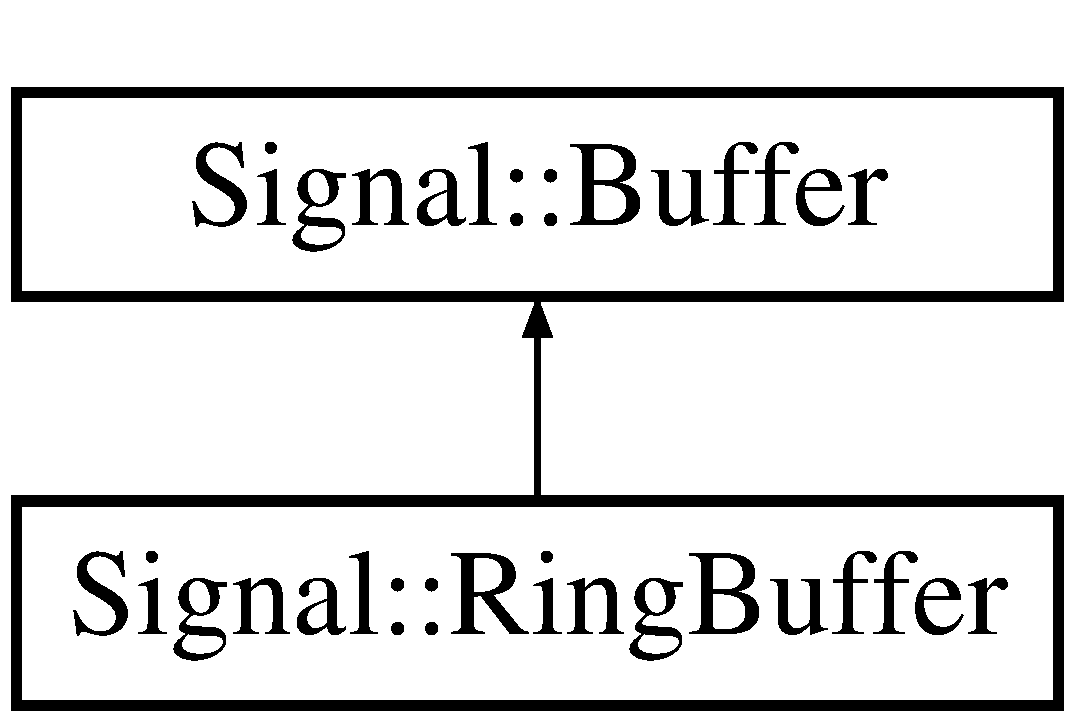
\includegraphics[height=2.000000cm]{classSignal_1_1Buffer}
\end{center}
\end{figure}
\subsection*{Public Member Functions}
\begin{DoxyCompactItemize}
\item 
\hyperlink{classSignal_1_1Buffer_ab558e80dac4ef396b9c9310fd914936f}{Buffer} ()
\item 
\hyperlink{classSignal_1_1Buffer_a002c329b3f2b4eaa388b27cc0796f68f}{Buffer} (size\+\_\+t size)
\item 
\hyperlink{classSignal_1_1Buffer_a89a0e919b2aa5f46f2c44137443128fc}{Buffer} (\hyperlink{classSignal_1_1Buffer}{Buffer} const \&other)
\item 
\hyperlink{classSignal_1_1Buffer}{Buffer} \& \hyperlink{classSignal_1_1Buffer_a9f9f08e2cdf35d15164997455303a2d9}{operator=} (\hyperlink{classSignal_1_1Buffer}{Buffer} const \&other)
\item 
virtual \hyperlink{classSignal_1_1Buffer_aa0a51349fdc5b8d41183e7971e8e799b}{$\sim$\+Buffer} ()
\item 
\hyperlink{classSignal_1_1Sample}{Signal\+::\+Sample} \& \hyperlink{classSignal_1_1Buffer_a0b4ced776c42720b214f6054fa21547a}{operator\mbox{[}$\,$\mbox{]}} (size\+\_\+t const \&index)
\item 
size\+\_\+t const \& \hyperlink{classSignal_1_1Buffer_ad0350078d641ed5cb15a9401d9d20ffe}{Size} () const 
\end{DoxyCompactItemize}
\subsection*{Protected Attributes}
\begin{DoxyCompactItemize}
\item 
\hyperlink{classSignal_1_1Sample}{Signal\+::\+Sample} $\ast$ \hyperlink{classSignal_1_1Buffer_ae88831d6fdf8fd7591d5dd7f79531d5f}{\+\_\+buffer}
\item 
size\+\_\+t \hyperlink{classSignal_1_1Buffer_ab4c8969e972323306ee51538ad70577b}{\+\_\+size}
\end{DoxyCompactItemize}


\subsection{Detailed Description}


Definition at line 18 of file Buffer.\+h.



\subsection{Constructor \& Destructor Documentation}
\hypertarget{classSignal_1_1Buffer_ab558e80dac4ef396b9c9310fd914936f}{\index{Signal\+::\+Buffer@{Signal\+::\+Buffer}!Buffer@{Buffer}}
\index{Buffer@{Buffer}!Signal\+::\+Buffer@{Signal\+::\+Buffer}}
\subsubsection[{Buffer}]{\setlength{\rightskip}{0pt plus 5cm}Signal\+::\+Buffer\+::\+Buffer (
\begin{DoxyParamCaption}
{}
\end{DoxyParamCaption}
)}}\label{classSignal_1_1Buffer_ab558e80dac4ef396b9c9310fd914936f}


Definition at line 13 of file Buffer.\+cpp.


\begin{DoxyCode}
13 :\hyperlink{classSignal_1_1Buffer_ab4c8969e972323306ee51538ad70577b}{\_size}(0),\hyperlink{classSignal_1_1Buffer_ae88831d6fdf8fd7591d5dd7f79531d5f}{\_buffer}(\textcolor{keyword}{nullptr})\{\}
\end{DoxyCode}
\hypertarget{classSignal_1_1Buffer_a002c329b3f2b4eaa388b27cc0796f68f}{\index{Signal\+::\+Buffer@{Signal\+::\+Buffer}!Buffer@{Buffer}}
\index{Buffer@{Buffer}!Signal\+::\+Buffer@{Signal\+::\+Buffer}}
\subsubsection[{Buffer}]{\setlength{\rightskip}{0pt plus 5cm}Signal\+::\+Buffer\+::\+Buffer (
\begin{DoxyParamCaption}
\item[{size\+\_\+t}]{size}
\end{DoxyParamCaption}
)}}\label{classSignal_1_1Buffer_a002c329b3f2b4eaa388b27cc0796f68f}


Definition at line 14 of file Buffer.\+cpp.


\begin{DoxyCode}
14 :\hyperlink{classSignal_1_1Buffer_ab4c8969e972323306ee51538ad70577b}{\_size}(size),\hyperlink{classSignal_1_1Buffer_ae88831d6fdf8fd7591d5dd7f79531d5f}{\_buffer}(\textcolor{keyword}{new} \hyperlink{classSignal_1_1Sample}{Signal::Sample}[size])\{\}
\end{DoxyCode}
\hypertarget{classSignal_1_1Buffer_a89a0e919b2aa5f46f2c44137443128fc}{\index{Signal\+::\+Buffer@{Signal\+::\+Buffer}!Buffer@{Buffer}}
\index{Buffer@{Buffer}!Signal\+::\+Buffer@{Signal\+::\+Buffer}}
\subsubsection[{Buffer}]{\setlength{\rightskip}{0pt plus 5cm}Signal\+::\+Buffer\+::\+Buffer (
\begin{DoxyParamCaption}
\item[{{\bf Buffer} const \&}]{other}
\end{DoxyParamCaption}
)}}\label{classSignal_1_1Buffer_a89a0e919b2aa5f46f2c44137443128fc}


Definition at line 15 of file Buffer.\+cpp.


\begin{DoxyCode}
15                                         \{
16     \hyperlink{classSignal_1_1Buffer_ae88831d6fdf8fd7591d5dd7f79531d5f}{\_buffer} = \textcolor{keyword}{new} \hyperlink{classSignal_1_1Sample}{Signal::Sample}[\hyperlink{classSignal_1_1Buffer_ab4c8969e972323306ee51538ad70577b}{\_size}];
17     \hyperlink{classSignal_1_1Buffer_ab4c8969e972323306ee51538ad70577b}{\_size} = other.\_size;
18     *\textcolor{keyword}{this} = other;
19 \}
\end{DoxyCode}
\hypertarget{classSignal_1_1Buffer_aa0a51349fdc5b8d41183e7971e8e799b}{\index{Signal\+::\+Buffer@{Signal\+::\+Buffer}!````~Buffer@{$\sim$\+Buffer}}
\index{````~Buffer@{$\sim$\+Buffer}!Signal\+::\+Buffer@{Signal\+::\+Buffer}}
\subsubsection[{$\sim$\+Buffer}]{\setlength{\rightskip}{0pt plus 5cm}Signal\+::\+Buffer\+::$\sim$\+Buffer (
\begin{DoxyParamCaption}
{}
\end{DoxyParamCaption}
)\hspace{0.3cm}{\ttfamily [virtual]}}}\label{classSignal_1_1Buffer_aa0a51349fdc5b8d41183e7971e8e799b}


Definition at line 33 of file Buffer.\+cpp.


\begin{DoxyCode}
33                      \{
34     \textcolor{keywordflow}{if} (\hyperlink{classSignal_1_1Buffer_ae88831d6fdf8fd7591d5dd7f79531d5f}{\_buffer}!=\textcolor{keyword}{nullptr}) \{
35         \textcolor{keyword}{delete} [] \hyperlink{classSignal_1_1Buffer_ae88831d6fdf8fd7591d5dd7f79531d5f}{\_buffer};
36     \}
37 \}
\end{DoxyCode}


\subsection{Member Function Documentation}
\hypertarget{classSignal_1_1Buffer_a9f9f08e2cdf35d15164997455303a2d9}{\index{Signal\+::\+Buffer@{Signal\+::\+Buffer}!operator=@{operator=}}
\index{operator=@{operator=}!Signal\+::\+Buffer@{Signal\+::\+Buffer}}
\subsubsection[{operator=}]{\setlength{\rightskip}{0pt plus 5cm}{\bf Signal\+::\+Buffer} \& Signal\+::\+Buffer\+::operator= (
\begin{DoxyParamCaption}
\item[{{\bf Buffer} const \&}]{other}
\end{DoxyParamCaption}
)}}\label{classSignal_1_1Buffer_a9f9f08e2cdf35d15164997455303a2d9}


Definition at line 20 of file Buffer.\+cpp.


\begin{DoxyCode}
20                                                         \{
21     \textcolor{keywordflow}{if} (\hyperlink{classSignal_1_1Buffer_ab4c8969e972323306ee51538ad70577b}{\_size}!=other.\_size) \{
22         \textcolor{keywordflow}{if} (\hyperlink{classSignal_1_1Buffer_ae88831d6fdf8fd7591d5dd7f79531d5f}{\_buffer}!=\textcolor{keyword}{nullptr}) \{
23             \textcolor{keyword}{delete} [] \hyperlink{classSignal_1_1Buffer_ae88831d6fdf8fd7591d5dd7f79531d5f}{\_buffer};
24         \}
25         \hyperlink{classSignal_1_1Buffer_ab4c8969e972323306ee51538ad70577b}{\_size} = other.\_size;
26         \hyperlink{classSignal_1_1Buffer_ae88831d6fdf8fd7591d5dd7f79531d5f}{\_buffer} = \textcolor{keyword}{new} \hyperlink{classSignal_1_1Sample}{Signal::Sample}[\hyperlink{classSignal_1_1Buffer_ab4c8969e972323306ee51538ad70577b}{\_size}];
27     \}
28     \textcolor{keywordflow}{for} (\textcolor{keywordtype}{int} i=0; i<\hyperlink{classSignal_1_1Buffer_ab4c8969e972323306ee51538ad70577b}{\_size}; ++i) \{
29         \hyperlink{classSignal_1_1Buffer_ae88831d6fdf8fd7591d5dd7f79531d5f}{\_buffer}[i] = other.\hyperlink{classSignal_1_1Sample_ad609d308b1c36b007bd8210d316c070b}{\_buffer}[i];
30     \}
31     \textcolor{keywordflow}{return} *\textcolor{keyword}{this};
32 \}
\end{DoxyCode}
\hypertarget{classSignal_1_1Buffer_a0b4ced776c42720b214f6054fa21547a}{\index{Signal\+::\+Buffer@{Signal\+::\+Buffer}!operator\mbox{[}$\,$\mbox{]}@{operator[]}}
\index{operator\mbox{[}$\,$\mbox{]}@{operator[]}!Signal\+::\+Buffer@{Signal\+::\+Buffer}}
\subsubsection[{operator[]}]{\setlength{\rightskip}{0pt plus 5cm}{\bf Signal\+::\+Sample} \& Signal\+::\+Buffer\+::operator\mbox{[}$\,$\mbox{]} (
\begin{DoxyParamCaption}
\item[{size\+\_\+t const \&}]{index}
\end{DoxyParamCaption}
)}}\label{classSignal_1_1Buffer_a0b4ced776c42720b214f6054fa21547a}


Definition at line 38 of file Buffer.\+cpp.


\begin{DoxyCode}
38                                                          \{
39 \textcolor{preprocessor}{#ifdef DEBUG}
40     assert(index<\hyperlink{classSignal_1_1Buffer_ab4c8969e972323306ee51538ad70577b}{\_size});
41 \textcolor{preprocessor}{#endif}
42     \textcolor{keywordflow}{return} \hyperlink{classSignal_1_1Buffer_ae88831d6fdf8fd7591d5dd7f79531d5f}{\_buffer}[index];
43 \}
\end{DoxyCode}
\hypertarget{classSignal_1_1Buffer_ad0350078d641ed5cb15a9401d9d20ffe}{\index{Signal\+::\+Buffer@{Signal\+::\+Buffer}!Size@{Size}}
\index{Size@{Size}!Signal\+::\+Buffer@{Signal\+::\+Buffer}}
\subsubsection[{Size}]{\setlength{\rightskip}{0pt plus 5cm}size\+\_\+t const \& Signal\+::\+Buffer\+::\+Size (
\begin{DoxyParamCaption}
{}
\end{DoxyParamCaption}
) const\hspace{0.3cm}{\ttfamily [inline]}}}\label{classSignal_1_1Buffer_ad0350078d641ed5cb15a9401d9d20ffe}


Definition at line 31 of file Buffer.\+h.


\begin{DoxyCode}
31                                           \{
32         \textcolor{keywordflow}{return} \hyperlink{classSignal_1_1Buffer_ab4c8969e972323306ee51538ad70577b}{\_size};
33     \}
\end{DoxyCode}


\subsection{Member Data Documentation}
\hypertarget{classSignal_1_1Buffer_ae88831d6fdf8fd7591d5dd7f79531d5f}{\index{Signal\+::\+Buffer@{Signal\+::\+Buffer}!\+\_\+buffer@{\+\_\+buffer}}
\index{\+\_\+buffer@{\+\_\+buffer}!Signal\+::\+Buffer@{Signal\+::\+Buffer}}
\subsubsection[{\+\_\+buffer}]{\setlength{\rightskip}{0pt plus 5cm}{\bf Signal\+::\+Sample}$\ast$ Signal\+::\+Buffer\+::\+\_\+buffer\hspace{0.3cm}{\ttfamily [protected]}}}\label{classSignal_1_1Buffer_ae88831d6fdf8fd7591d5dd7f79531d5f}


Definition at line 28 of file Buffer.\+h.

\hypertarget{classSignal_1_1Buffer_ab4c8969e972323306ee51538ad70577b}{\index{Signal\+::\+Buffer@{Signal\+::\+Buffer}!\+\_\+size@{\+\_\+size}}
\index{\+\_\+size@{\+\_\+size}!Signal\+::\+Buffer@{Signal\+::\+Buffer}}
\subsubsection[{\+\_\+size}]{\setlength{\rightskip}{0pt plus 5cm}size\+\_\+t Signal\+::\+Buffer\+::\+\_\+size\hspace{0.3cm}{\ttfamily [protected]}}}\label{classSignal_1_1Buffer_ab4c8969e972323306ee51538ad70577b}


Definition at line 29 of file Buffer.\+h.



The documentation for this class was generated from the following files\+:\begin{DoxyCompactItemize}
\item 
/\+Users/alexanderzywicki/\+Documents/\+School\+\_\+\+Stuff/\+Fall\+\_\+2014/\+Digital\+\_\+\+Signal\+\_\+\+Generation\+\_\+and\+\_\+\+Analysis/src/include/\hyperlink{Buffer_8h}{Buffer.\+h}\item 
/\+Users/alexanderzywicki/\+Documents/\+School\+\_\+\+Stuff/\+Fall\+\_\+2014/\+Digital\+\_\+\+Signal\+\_\+\+Generation\+\_\+and\+\_\+\+Analysis/src/\hyperlink{Buffer_8cpp}{Buffer.\+cpp}\end{DoxyCompactItemize}

\hypertarget{classSignal_1_1ClassicGenerator}{\section{Signal\+:\+:Classic\+Generator Class Reference}
\label{classSignal_1_1ClassicGenerator}\index{Signal\+::\+Classic\+Generator@{Signal\+::\+Classic\+Generator}}
}


{\ttfamily \#include $<$Classic\+Generator.\+h$>$}

Inheritance diagram for Signal\+:\+:Classic\+Generator\+:\begin{figure}[H]
\begin{center}
\leavevmode
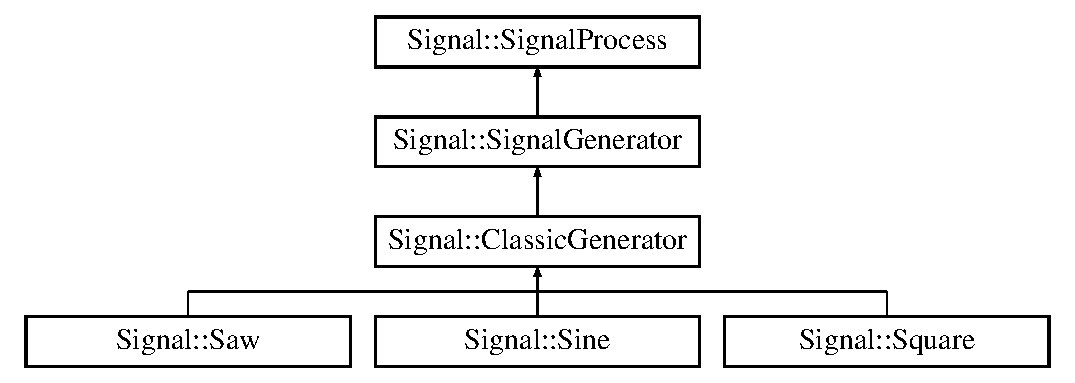
\includegraphics[height=4.000000cm]{classSignal_1_1ClassicGenerator}
\end{center}
\end{figure}
\subsection*{Public Member Functions}
\begin{DoxyCompactItemize}
\item 
\hyperlink{classSignal_1_1ClassicGenerator_a7e4478904de77156deccb1515f6985cb}{Classic\+Generator} ()
\item 
\hyperlink{classSignal_1_1ClassicGenerator_aa8e7631c9a4a72d42bbe560c02ed7358}{Classic\+Generator} (double const \&frequency, double const \&phase\+\_\+offset)
\item 
virtual \hyperlink{classSignal_1_1ClassicGenerator_a6659174adf402df341e3c0f94564fd37}{$\sim$\+Classic\+Generator} ()
\item 
virtual bool \hyperlink{classSignal_1_1ClassicGenerator_a4a62f329b9cd64d92b07f53c4d593356}{Perform} (\hyperlink{classSignal_1_1Sample}{Sample} \&signal)
\item 
virtual bool \hyperlink{classSignal_1_1ClassicGenerator_a308c13baa66020d44c2227bd58db4b4f}{Perform} (\hyperlink{classSignal_1_1RingBuffer}{Ring\+Buffer} \&signal)
\item 
virtual double const \& \hyperlink{classSignal_1_1SignalGenerator_a96af42ee68f94e9b04d034fd68b73ecd}{Frequency} () const 
\item 
virtual double const \& \hyperlink{classSignal_1_1SignalGenerator_af83b532bf3ddc3637c2fd7a1dfd095cb}{Frequency} (double const \&value)
\item 
virtual double const \& \hyperlink{classSignal_1_1SignalGenerator_ac2538ec946f001e394d2416fda698d1c}{Phase\+Offset} () const 
\item 
virtual double const \& \hyperlink{classSignal_1_1SignalGenerator_ac6a103ff72beaa338f6d18c812522d78}{Phase\+Offset} (double const \&value)
\end{DoxyCompactItemize}
\subsection*{Protected Member Functions}
\begin{DoxyCompactItemize}
\item 
unsigned long \hyperlink{classSignal_1_1ClassicGenerator_a7457e912d428de4e3fc27ec7fc49890e}{\+\_\+max\+Harms} (double \+\_\+frq)
\item 
double \hyperlink{classSignal_1_1ClassicGenerator_a255330ce8049b6e6d101b8d356cebe3d}{\+\_\+pstep} ()
\item 
double \hyperlink{classSignal_1_1ClassicGenerator_a6571276f584ff0be3862243d0f103a92}{\+\_\+pstep\+\_\+rad} ()
\item 
void \hyperlink{classSignal_1_1ClassicGenerator_a6454565b655bff7b8335735c2fabb4af}{\+\_\+psync} ()
\end{DoxyCompactItemize}
\subsection*{Protected Attributes}
\begin{DoxyCompactItemize}
\item 
\hyperlink{classSignal_1_1Sample}{Sample} \hyperlink{classSignal_1_1ClassicGenerator_a40313d0d806d6e44af7d41b3ef3a0822}{\+\_\+sample}
\item 
\hyperlink{classSignal_1_1Sample}{Sample} \hyperlink{classSignal_1_1ClassicGenerator_a1214faf589eccb01631700723900bbf9}{\+\_\+storage}
\item 
double \hyperlink{classSignal_1_1ClassicGenerator_ade9b66bc49d2d2f40a1390fc6374b8b2}{\+\_\+phasor}
\item 
double \hyperlink{classSignal_1_1SignalGenerator_a7f107461333bce68c5dad412db96a8c2}{\+\_\+frequency}
\item 
double \hyperlink{classSignal_1_1SignalGenerator_a85a4702347352bab1c71e0a8df8437d6}{\+\_\+f\+Hertz}
\item 
double \hyperlink{classSignal_1_1SignalGenerator_a6b4444d46747c8517171edbbf4b5588f}{\+\_\+phase\+\_\+offset}
\end{DoxyCompactItemize}


\subsection{Detailed Description}


Definition at line 24 of file Classic\+Generator.\+h.



\subsection{Constructor \& Destructor Documentation}
\hypertarget{classSignal_1_1ClassicGenerator_a7e4478904de77156deccb1515f6985cb}{\index{Signal\+::\+Classic\+Generator@{Signal\+::\+Classic\+Generator}!Classic\+Generator@{Classic\+Generator}}
\index{Classic\+Generator@{Classic\+Generator}!Signal\+::\+Classic\+Generator@{Signal\+::\+Classic\+Generator}}
\subsubsection[{Classic\+Generator}]{\setlength{\rightskip}{0pt plus 5cm}Signal\+::\+Classic\+Generator\+::\+Classic\+Generator (
\begin{DoxyParamCaption}
{}
\end{DoxyParamCaption}
)}}\label{classSignal_1_1ClassicGenerator_a7e4478904de77156deccb1515f6985cb}


Definition at line 11 of file Classic\+Generator.\+cpp.


\begin{DoxyCode}
11                                         :\hyperlink{classSignal_1_1SignalGenerator_a8c67c754d86e0363445d7fd271855e1a}{SignalGenerator}(),
      \hyperlink{classSignal_1_1ClassicGenerator_ade9b66bc49d2d2f40a1390fc6374b8b2}{\_phasor}(0)\{
12     
13 \}
\end{DoxyCode}
\hypertarget{classSignal_1_1ClassicGenerator_aa8e7631c9a4a72d42bbe560c02ed7358}{\index{Signal\+::\+Classic\+Generator@{Signal\+::\+Classic\+Generator}!Classic\+Generator@{Classic\+Generator}}
\index{Classic\+Generator@{Classic\+Generator}!Signal\+::\+Classic\+Generator@{Signal\+::\+Classic\+Generator}}
\subsubsection[{Classic\+Generator}]{\setlength{\rightskip}{0pt plus 5cm}Signal\+::\+Classic\+Generator\+::\+Classic\+Generator (
\begin{DoxyParamCaption}
\item[{double const \&}]{frequency, }
\item[{double const \&}]{phase\+\_\+offset}
\end{DoxyParamCaption}
)}}\label{classSignal_1_1ClassicGenerator_aa8e7631c9a4a72d42bbe560c02ed7358}


Definition at line 14 of file Classic\+Generator.\+cpp.


\begin{DoxyCode}
14 :\hyperlink{classSignal_1_1SignalGenerator_a8c67c754d86e0363445d7fd271855e1a}{SignalGenerator}(frequency,phase\_offset),\hyperlink{classSignal_1_1ClassicGenerator_ade9b66bc49d2d2f40a1390fc6374b8b2}{\_phasor}(0)\{\}
\end{DoxyCode}
\hypertarget{classSignal_1_1ClassicGenerator_a6659174adf402df341e3c0f94564fd37}{\index{Signal\+::\+Classic\+Generator@{Signal\+::\+Classic\+Generator}!````~Classic\+Generator@{$\sim$\+Classic\+Generator}}
\index{````~Classic\+Generator@{$\sim$\+Classic\+Generator}!Signal\+::\+Classic\+Generator@{Signal\+::\+Classic\+Generator}}
\subsubsection[{$\sim$\+Classic\+Generator}]{\setlength{\rightskip}{0pt plus 5cm}Signal\+::\+Classic\+Generator\+::$\sim$\+Classic\+Generator (
\begin{DoxyParamCaption}
{}
\end{DoxyParamCaption}
)\hspace{0.3cm}{\ttfamily [virtual]}}}\label{classSignal_1_1ClassicGenerator_a6659174adf402df341e3c0f94564fd37}


Definition at line 15 of file Classic\+Generator.\+cpp.


\begin{DoxyCode}
15 \{\}
\end{DoxyCode}


\subsection{Member Function Documentation}
\hypertarget{classSignal_1_1ClassicGenerator_a7457e912d428de4e3fc27ec7fc49890e}{\index{Signal\+::\+Classic\+Generator@{Signal\+::\+Classic\+Generator}!\+\_\+max\+Harms@{\+\_\+max\+Harms}}
\index{\+\_\+max\+Harms@{\+\_\+max\+Harms}!Signal\+::\+Classic\+Generator@{Signal\+::\+Classic\+Generator}}
\subsubsection[{\+\_\+max\+Harms}]{\setlength{\rightskip}{0pt plus 5cm}unsigned long Signal\+::\+Classic\+Generator\+::\+\_\+max\+Harms (
\begin{DoxyParamCaption}
\item[{double}]{\+\_\+frq}
\end{DoxyParamCaption}
)\hspace{0.3cm}{\ttfamily [inline]}, {\ttfamily [protected]}}}\label{classSignal_1_1ClassicGenerator_a7457e912d428de4e3fc27ec7fc49890e}


Definition at line 70 of file Classic\+Generator.\+h.


\begin{DoxyCode}
70                                                                \{
71         \textcolor{comment}{//double softLim = 0.45;}
72         \textcolor{comment}{//double hardLim = 0.5;}
73         \textcolor{keywordtype}{double} \_s = \hyperlink{namespaceSignal_ae7b1f222afc010e0f33f306f978fcde9}{Sample\_Rate}()* 0.45;
74         \_s/=\_frq;
75         \textcolor{keywordflow}{return} trunc(\_s);
76     \}
\end{DoxyCode}
\hypertarget{classSignal_1_1ClassicGenerator_a255330ce8049b6e6d101b8d356cebe3d}{\index{Signal\+::\+Classic\+Generator@{Signal\+::\+Classic\+Generator}!\+\_\+pstep@{\+\_\+pstep}}
\index{\+\_\+pstep@{\+\_\+pstep}!Signal\+::\+Classic\+Generator@{Signal\+::\+Classic\+Generator}}
\subsubsection[{\+\_\+pstep}]{\setlength{\rightskip}{0pt plus 5cm}double Signal\+::\+Classic\+Generator\+::\+\_\+pstep (
\begin{DoxyParamCaption}
{}
\end{DoxyParamCaption}
)\hspace{0.3cm}{\ttfamily [inline]}, {\ttfamily [protected]}}}\label{classSignal_1_1ClassicGenerator_a255330ce8049b6e6d101b8d356cebe3d}


Definition at line 57 of file Classic\+Generator.\+h.


\begin{DoxyCode}
57                                           \{
58         \textcolor{keywordtype}{double} value = \hyperlink{classSignal_1_1ClassicGenerator_ade9b66bc49d2d2f40a1390fc6374b8b2}{\_phasor};
59         \hyperlink{classSignal_1_1ClassicGenerator_ade9b66bc49d2d2f40a1390fc6374b8b2}{\_phasor}+=\hyperlink{classSignal_1_1SignalGenerator_a7f107461333bce68c5dad412db96a8c2}{\_frequency};
60         \hyperlink{classSignal_1_1ClassicGenerator_ade9b66bc49d2d2f40a1390fc6374b8b2}{\_phasor} = \hyperlink{classSignal_1_1ClassicGenerator_ade9b66bc49d2d2f40a1390fc6374b8b2}{\_phasor}-(\textcolor{keywordtype}{unsigned} long)\hyperlink{classSignal_1_1ClassicGenerator_ade9b66bc49d2d2f40a1390fc6374b8b2}{\_phasor};\textcolor{comment}{//cheaper %1}
61         \textcolor{keywordflow}{return} value;
62     \}
\end{DoxyCode}
\hypertarget{classSignal_1_1ClassicGenerator_a6571276f584ff0be3862243d0f103a92}{\index{Signal\+::\+Classic\+Generator@{Signal\+::\+Classic\+Generator}!\+\_\+pstep\+\_\+rad@{\+\_\+pstep\+\_\+rad}}
\index{\+\_\+pstep\+\_\+rad@{\+\_\+pstep\+\_\+rad}!Signal\+::\+Classic\+Generator@{Signal\+::\+Classic\+Generator}}
\subsubsection[{\+\_\+pstep\+\_\+rad}]{\setlength{\rightskip}{0pt plus 5cm}double Signal\+::\+Classic\+Generator\+::\+\_\+pstep\+\_\+rad (
\begin{DoxyParamCaption}
{}
\end{DoxyParamCaption}
)\hspace{0.3cm}{\ttfamily [inline]}, {\ttfamily [protected]}}}\label{classSignal_1_1ClassicGenerator_a6571276f584ff0be3862243d0f103a92}


Definition at line 63 of file Classic\+Generator.\+h.


\begin{DoxyCode}
63                                               \{
64         \textcolor{keywordflow}{return} \hyperlink{PI_8h_a4912c64aec0c943b7985db6cb61ff83a}{TWOPI} * \hyperlink{classSignal_1_1ClassicGenerator_a255330ce8049b6e6d101b8d356cebe3d}{\_pstep}();
65     \}
\end{DoxyCode}
\hypertarget{classSignal_1_1ClassicGenerator_a6454565b655bff7b8335735c2fabb4af}{\index{Signal\+::\+Classic\+Generator@{Signal\+::\+Classic\+Generator}!\+\_\+psync@{\+\_\+psync}}
\index{\+\_\+psync@{\+\_\+psync}!Signal\+::\+Classic\+Generator@{Signal\+::\+Classic\+Generator}}
\subsubsection[{\+\_\+psync}]{\setlength{\rightskip}{0pt plus 5cm}void Signal\+::\+Classic\+Generator\+::\+\_\+psync (
\begin{DoxyParamCaption}
{}
\end{DoxyParamCaption}
)\hspace{0.3cm}{\ttfamily [inline]}, {\ttfamily [protected]}}}\label{classSignal_1_1ClassicGenerator_a6454565b655bff7b8335735c2fabb4af}


Definition at line 66 of file Classic\+Generator.\+h.


\begin{DoxyCode}
66                                         \{
67         \hyperlink{classSignal_1_1ClassicGenerator_ade9b66bc49d2d2f40a1390fc6374b8b2}{\_phasor} = 0;
68     \}
\end{DoxyCode}
\hypertarget{classSignal_1_1SignalGenerator_a96af42ee68f94e9b04d034fd68b73ecd}{\index{Signal\+::\+Classic\+Generator@{Signal\+::\+Classic\+Generator}!Frequency@{Frequency}}
\index{Frequency@{Frequency}!Signal\+::\+Classic\+Generator@{Signal\+::\+Classic\+Generator}}
\subsubsection[{Frequency}]{\setlength{\rightskip}{0pt plus 5cm}double const \& Signal\+::\+Signal\+Generator\+::\+Frequency (
\begin{DoxyParamCaption}
{}
\end{DoxyParamCaption}
) const\hspace{0.3cm}{\ttfamily [virtual]}, {\ttfamily [inherited]}}}\label{classSignal_1_1SignalGenerator_a96af42ee68f94e9b04d034fd68b73ecd}


Definition at line 16 of file Signal\+Generator.\+cpp.


\begin{DoxyCode}
16                                                    \{
17     \textcolor{keywordflow}{return} \hyperlink{classSignal_1_1SignalGenerator_a85a4702347352bab1c71e0a8df8437d6}{\_fHertz};
18 \}
\end{DoxyCode}
\hypertarget{classSignal_1_1SignalGenerator_af83b532bf3ddc3637c2fd7a1dfd095cb}{\index{Signal\+::\+Classic\+Generator@{Signal\+::\+Classic\+Generator}!Frequency@{Frequency}}
\index{Frequency@{Frequency}!Signal\+::\+Classic\+Generator@{Signal\+::\+Classic\+Generator}}
\subsubsection[{Frequency}]{\setlength{\rightskip}{0pt plus 5cm}double const \& Signal\+::\+Signal\+Generator\+::\+Frequency (
\begin{DoxyParamCaption}
\item[{double const \&}]{value}
\end{DoxyParamCaption}
)\hspace{0.3cm}{\ttfamily [virtual]}, {\ttfamily [inherited]}}}\label{classSignal_1_1SignalGenerator_af83b532bf3ddc3637c2fd7a1dfd095cb}


Reimplemented in \hyperlink{classSignal_1_1BLIT_1_1BLIT_a59110620478308054d4c932c613e5cc6}{Signal\+::\+B\+L\+I\+T\+::\+B\+L\+I\+T}, \hyperlink{classSignal_1_1Saw_af91fd0d15b380c02e309705eaad46efd}{Signal\+::\+Saw}, and \hyperlink{classSignal_1_1Square_a19f966d5b1800f5487cdd164747b21c0}{Signal\+::\+Square}.



Definition at line 19 of file Signal\+Generator.\+cpp.


\begin{DoxyCode}
19                                                                  \{
20     \hyperlink{classSignal_1_1SignalGenerator_a85a4702347352bab1c71e0a8df8437d6}{\_fHertz} = value;
21     \hyperlink{classSignal_1_1SignalGenerator_a7f107461333bce68c5dad412db96a8c2}{\_frequency} = \hyperlink{classSignal_1_1SignalGenerator_a85a4702347352bab1c71e0a8df8437d6}{\_fHertz}/\hyperlink{namespaceSignal_ae7b1f222afc010e0f33f306f978fcde9}{Sample\_Rate}();
22     \textcolor{keywordflow}{return} \hyperlink{classSignal_1_1SignalGenerator_a85a4702347352bab1c71e0a8df8437d6}{\_fHertz};
23 \}
\end{DoxyCode}
\hypertarget{classSignal_1_1ClassicGenerator_a4a62f329b9cd64d92b07f53c4d593356}{\index{Signal\+::\+Classic\+Generator@{Signal\+::\+Classic\+Generator}!Perform@{Perform}}
\index{Perform@{Perform}!Signal\+::\+Classic\+Generator@{Signal\+::\+Classic\+Generator}}
\subsubsection[{Perform}]{\setlength{\rightskip}{0pt plus 5cm}bool Signal\+::\+Classic\+Generator\+::\+Perform (
\begin{DoxyParamCaption}
\item[{{\bf Sample} \&}]{signal}
\end{DoxyParamCaption}
)\hspace{0.3cm}{\ttfamily [inline]}, {\ttfamily [virtual]}}}\label{classSignal_1_1ClassicGenerator_a4a62f329b9cd64d92b07f53c4d593356}


Reimplemented from \hyperlink{classSignal_1_1SignalGenerator_a2cd9061c5ae40a392a9476551b4379f3}{Signal\+::\+Signal\+Generator}.



Reimplemented in \hyperlink{classSignal_1_1Sine_a8f7c74c35cfd87b490d84a7a75c35691}{Signal\+::\+Sine}, \hyperlink{classSignal_1_1Saw_a6fb3216b94fea4daa83b27f5de194fa0}{Signal\+::\+Saw}, and \hyperlink{classSignal_1_1Square_a584e1b867aed4cc4a808d8fb844387bc}{Signal\+::\+Square}.



Definition at line 48 of file Classic\+Generator.\+h.


\begin{DoxyCode}
48                                                        \{
49         signal = 0;
50         \textcolor{keywordflow}{return} \textcolor{keyword}{false};
51     \}
\end{DoxyCode}
\hypertarget{classSignal_1_1ClassicGenerator_a308c13baa66020d44c2227bd58db4b4f}{\index{Signal\+::\+Classic\+Generator@{Signal\+::\+Classic\+Generator}!Perform@{Perform}}
\index{Perform@{Perform}!Signal\+::\+Classic\+Generator@{Signal\+::\+Classic\+Generator}}
\subsubsection[{Perform}]{\setlength{\rightskip}{0pt plus 5cm}bool Signal\+::\+Classic\+Generator\+::\+Perform (
\begin{DoxyParamCaption}
\item[{{\bf Ring\+Buffer} \&}]{signal}
\end{DoxyParamCaption}
)\hspace{0.3cm}{\ttfamily [inline]}, {\ttfamily [virtual]}}}\label{classSignal_1_1ClassicGenerator_a308c13baa66020d44c2227bd58db4b4f}


Reimplemented from \hyperlink{classSignal_1_1SignalGenerator_a126d52dd9b6b14d33efc624e2c89284e}{Signal\+::\+Signal\+Generator}.



Reimplemented in \hyperlink{classSignal_1_1Sine_ac0a6c6e24f830446ea75de3a392f7e06}{Signal\+::\+Sine}, \hyperlink{classSignal_1_1Saw_a0d0d374c9b5a3f73f48e9fb1c444b0ca}{Signal\+::\+Saw}, and \hyperlink{classSignal_1_1Square_ab398eba1087030249d04f27a364f45ed}{Signal\+::\+Square}.



Definition at line 52 of file Classic\+Generator.\+h.


\begin{DoxyCode}
52                                                            \{
53         signal.Flush();
54         \textcolor{keywordflow}{return} \textcolor{keyword}{false};
55     \}
\end{DoxyCode}
\hypertarget{classSignal_1_1SignalGenerator_ac2538ec946f001e394d2416fda698d1c}{\index{Signal\+::\+Classic\+Generator@{Signal\+::\+Classic\+Generator}!Phase\+Offset@{Phase\+Offset}}
\index{Phase\+Offset@{Phase\+Offset}!Signal\+::\+Classic\+Generator@{Signal\+::\+Classic\+Generator}}
\subsubsection[{Phase\+Offset}]{\setlength{\rightskip}{0pt plus 5cm}double const \& Signal\+::\+Signal\+Generator\+::\+Phase\+Offset (
\begin{DoxyParamCaption}
{}
\end{DoxyParamCaption}
) const\hspace{0.3cm}{\ttfamily [virtual]}, {\ttfamily [inherited]}}}\label{classSignal_1_1SignalGenerator_ac2538ec946f001e394d2416fda698d1c}


Definition at line 24 of file Signal\+Generator.\+cpp.


\begin{DoxyCode}
24                                                      \{
25     \textcolor{keywordflow}{return} \hyperlink{classSignal_1_1SignalGenerator_a6b4444d46747c8517171edbbf4b5588f}{\_phase\_offset};
26 \}
\end{DoxyCode}
\hypertarget{classSignal_1_1SignalGenerator_ac6a103ff72beaa338f6d18c812522d78}{\index{Signal\+::\+Classic\+Generator@{Signal\+::\+Classic\+Generator}!Phase\+Offset@{Phase\+Offset}}
\index{Phase\+Offset@{Phase\+Offset}!Signal\+::\+Classic\+Generator@{Signal\+::\+Classic\+Generator}}
\subsubsection[{Phase\+Offset}]{\setlength{\rightskip}{0pt plus 5cm}double const \& Signal\+::\+Signal\+Generator\+::\+Phase\+Offset (
\begin{DoxyParamCaption}
\item[{double const \&}]{value}
\end{DoxyParamCaption}
)\hspace{0.3cm}{\ttfamily [virtual]}, {\ttfamily [inherited]}}}\label{classSignal_1_1SignalGenerator_ac6a103ff72beaa338f6d18c812522d78}


Definition at line 27 of file Signal\+Generator.\+cpp.


\begin{DoxyCode}
27                                                                    \{
28     \hyperlink{classSignal_1_1SignalGenerator_a6b4444d46747c8517171edbbf4b5588f}{\_phase\_offset} = value;
29     \textcolor{keywordflow}{return} \hyperlink{classSignal_1_1SignalGenerator_a6b4444d46747c8517171edbbf4b5588f}{\_phase\_offset};
30 \}
\end{DoxyCode}


\subsection{Member Data Documentation}
\hypertarget{classSignal_1_1SignalGenerator_a85a4702347352bab1c71e0a8df8437d6}{\index{Signal\+::\+Classic\+Generator@{Signal\+::\+Classic\+Generator}!\+\_\+f\+Hertz@{\+\_\+f\+Hertz}}
\index{\+\_\+f\+Hertz@{\+\_\+f\+Hertz}!Signal\+::\+Classic\+Generator@{Signal\+::\+Classic\+Generator}}
\subsubsection[{\+\_\+f\+Hertz}]{\setlength{\rightskip}{0pt plus 5cm}double Signal\+::\+Signal\+Generator\+::\+\_\+f\+Hertz\hspace{0.3cm}{\ttfamily [protected]}, {\ttfamily [inherited]}}}\label{classSignal_1_1SignalGenerator_a85a4702347352bab1c71e0a8df8437d6}


Definition at line 34 of file Signal\+Generator.\+h.

\hypertarget{classSignal_1_1SignalGenerator_a7f107461333bce68c5dad412db96a8c2}{\index{Signal\+::\+Classic\+Generator@{Signal\+::\+Classic\+Generator}!\+\_\+frequency@{\+\_\+frequency}}
\index{\+\_\+frequency@{\+\_\+frequency}!Signal\+::\+Classic\+Generator@{Signal\+::\+Classic\+Generator}}
\subsubsection[{\+\_\+frequency}]{\setlength{\rightskip}{0pt plus 5cm}double Signal\+::\+Signal\+Generator\+::\+\_\+frequency\hspace{0.3cm}{\ttfamily [protected]}, {\ttfamily [inherited]}}}\label{classSignal_1_1SignalGenerator_a7f107461333bce68c5dad412db96a8c2}


Definition at line 33 of file Signal\+Generator.\+h.

\hypertarget{classSignal_1_1SignalGenerator_a6b4444d46747c8517171edbbf4b5588f}{\index{Signal\+::\+Classic\+Generator@{Signal\+::\+Classic\+Generator}!\+\_\+phase\+\_\+offset@{\+\_\+phase\+\_\+offset}}
\index{\+\_\+phase\+\_\+offset@{\+\_\+phase\+\_\+offset}!Signal\+::\+Classic\+Generator@{Signal\+::\+Classic\+Generator}}
\subsubsection[{\+\_\+phase\+\_\+offset}]{\setlength{\rightskip}{0pt plus 5cm}double Signal\+::\+Signal\+Generator\+::\+\_\+phase\+\_\+offset\hspace{0.3cm}{\ttfamily [protected]}, {\ttfamily [inherited]}}}\label{classSignal_1_1SignalGenerator_a6b4444d46747c8517171edbbf4b5588f}


Definition at line 35 of file Signal\+Generator.\+h.

\hypertarget{classSignal_1_1ClassicGenerator_ade9b66bc49d2d2f40a1390fc6374b8b2}{\index{Signal\+::\+Classic\+Generator@{Signal\+::\+Classic\+Generator}!\+\_\+phasor@{\+\_\+phasor}}
\index{\+\_\+phasor@{\+\_\+phasor}!Signal\+::\+Classic\+Generator@{Signal\+::\+Classic\+Generator}}
\subsubsection[{\+\_\+phasor}]{\setlength{\rightskip}{0pt plus 5cm}double Signal\+::\+Classic\+Generator\+::\+\_\+phasor\hspace{0.3cm}{\ttfamily [protected]}}}\label{classSignal_1_1ClassicGenerator_ade9b66bc49d2d2f40a1390fc6374b8b2}


Definition at line 41 of file Classic\+Generator.\+h.

\hypertarget{classSignal_1_1ClassicGenerator_a40313d0d806d6e44af7d41b3ef3a0822}{\index{Signal\+::\+Classic\+Generator@{Signal\+::\+Classic\+Generator}!\+\_\+sample@{\+\_\+sample}}
\index{\+\_\+sample@{\+\_\+sample}!Signal\+::\+Classic\+Generator@{Signal\+::\+Classic\+Generator}}
\subsubsection[{\+\_\+sample}]{\setlength{\rightskip}{0pt plus 5cm}{\bf Sample} Signal\+::\+Classic\+Generator\+::\+\_\+sample\hspace{0.3cm}{\ttfamily [protected]}}}\label{classSignal_1_1ClassicGenerator_a40313d0d806d6e44af7d41b3ef3a0822}


Definition at line 34 of file Classic\+Generator.\+h.

\hypertarget{classSignal_1_1ClassicGenerator_a1214faf589eccb01631700723900bbf9}{\index{Signal\+::\+Classic\+Generator@{Signal\+::\+Classic\+Generator}!\+\_\+storage@{\+\_\+storage}}
\index{\+\_\+storage@{\+\_\+storage}!Signal\+::\+Classic\+Generator@{Signal\+::\+Classic\+Generator}}
\subsubsection[{\+\_\+storage}]{\setlength{\rightskip}{0pt plus 5cm}{\bf Sample} Signal\+::\+Classic\+Generator\+::\+\_\+storage\hspace{0.3cm}{\ttfamily [protected]}}}\label{classSignal_1_1ClassicGenerator_a1214faf589eccb01631700723900bbf9}


Definition at line 35 of file Classic\+Generator.\+h.



The documentation for this class was generated from the following files\+:\begin{DoxyCompactItemize}
\item 
/\+Users/alexanderzywicki/\+Documents/\+School\+\_\+\+Stuff/\+Fall\+\_\+2014/\+Digital\+\_\+\+Signal\+\_\+\+Generation\+\_\+and\+\_\+\+Analysis/src/include/\hyperlink{ClassicGenerator_8h}{Classic\+Generator.\+h}\item 
/\+Users/alexanderzywicki/\+Documents/\+School\+\_\+\+Stuff/\+Fall\+\_\+2014/\+Digital\+\_\+\+Signal\+\_\+\+Generation\+\_\+and\+\_\+\+Analysis/src/\hyperlink{ClassicGenerator_8cpp}{Classic\+Generator.\+cpp}\end{DoxyCompactItemize}

\hypertarget{classBackend_1_1HarmonicTable}{\section{Backend\+:\+:Harmonic\+Table Class Reference}
\label{classBackend_1_1HarmonicTable}\index{Backend\+::\+Harmonic\+Table@{Backend\+::\+Harmonic\+Table}}
}


{\ttfamily \#include $<$Harmonic\+Table.\+h$>$}

\subsection*{Public Member Functions}
\begin{DoxyCompactItemize}
\item 
\hyperlink{classBackend_1_1HarmonicTable_a3ea23b72d602447940c3d97ba75e5902}{Harmonic\+Table} ()
\item 
\hyperlink{classBackend_1_1HarmonicTable_a1c3662131adb3c8e64d1ad1cd8a65a20}{$\sim$\+Harmonic\+Table} ()
\item 
double const \& \hyperlink{classBackend_1_1HarmonicTable_a6b7336f4f6184337350f282d5b0c5467}{Saw} (unsigned short const \&index)
\item 
double const \& \hyperlink{classBackend_1_1HarmonicTable_a97f9bbd2ba8612793776b2102f221c33}{Triangle} (unsigned short const \&index)
\end{DoxyCompactItemize}
\subsection*{Protected Member Functions}
\begin{DoxyCompactItemize}
\item 
void \hyperlink{classBackend_1_1HarmonicTable_a3b69fe79e5ddd9abfc13fc9a16de80c8}{fill\+Saw} ()
\item 
void \hyperlink{classBackend_1_1HarmonicTable_a581dd50f5e6502945e8b494cccab7244}{fill\+Tri} ()
\end{DoxyCompactItemize}
\subsection*{Protected Attributes}
\begin{DoxyCompactItemize}
\item 
double \hyperlink{classBackend_1_1HarmonicTable_a464db802494a562d2c9d0840ee6d1483}{\+\_\+saw} \mbox{[}8192\mbox{]}
\item 
double \hyperlink{classBackend_1_1HarmonicTable_a8e6fa80e2428d690a5716ae2815fd032}{\+\_\+triangle} \mbox{[}8192\mbox{]}
\item 
const short \hyperlink{classBackend_1_1HarmonicTable_a94c9f17b8fd4b514d145fbb8b0ed63dd}{\+\_\+size} =8192
\end{DoxyCompactItemize}


\subsection{Detailed Description}


Definition at line 19 of file Harmonic\+Table.\+h.



\subsection{Constructor \& Destructor Documentation}
\hypertarget{classBackend_1_1HarmonicTable_a3ea23b72d602447940c3d97ba75e5902}{\index{Backend\+::\+Harmonic\+Table@{Backend\+::\+Harmonic\+Table}!Harmonic\+Table@{Harmonic\+Table}}
\index{Harmonic\+Table@{Harmonic\+Table}!Backend\+::\+Harmonic\+Table@{Backend\+::\+Harmonic\+Table}}
\subsubsection[{Harmonic\+Table}]{\setlength{\rightskip}{0pt plus 5cm}Backend\+::\+Harmonic\+Table\+::\+Harmonic\+Table (
\begin{DoxyParamCaption}
{}
\end{DoxyParamCaption}
)}}\label{classBackend_1_1HarmonicTable_a3ea23b72d602447940c3d97ba75e5902}


Definition at line 12 of file Harmonic\+Table.\+cpp.


\begin{DoxyCode}
12                                    \{
13     \hyperlink{classBackend_1_1HarmonicTable_a3b69fe79e5ddd9abfc13fc9a16de80c8}{fillSaw}();
14     \hyperlink{classBackend_1_1HarmonicTable_a581dd50f5e6502945e8b494cccab7244}{fillTri}();
15 \}
\end{DoxyCode}
\hypertarget{classBackend_1_1HarmonicTable_a1c3662131adb3c8e64d1ad1cd8a65a20}{\index{Backend\+::\+Harmonic\+Table@{Backend\+::\+Harmonic\+Table}!````~Harmonic\+Table@{$\sim$\+Harmonic\+Table}}
\index{````~Harmonic\+Table@{$\sim$\+Harmonic\+Table}!Backend\+::\+Harmonic\+Table@{Backend\+::\+Harmonic\+Table}}
\subsubsection[{$\sim$\+Harmonic\+Table}]{\setlength{\rightskip}{0pt plus 5cm}Backend\+::\+Harmonic\+Table\+::$\sim$\+Harmonic\+Table (
\begin{DoxyParamCaption}
{}
\end{DoxyParamCaption}
)}}\label{classBackend_1_1HarmonicTable_a1c3662131adb3c8e64d1ad1cd8a65a20}


Definition at line 16 of file Harmonic\+Table.\+cpp.


\begin{DoxyCode}
16                                     \{
17     
18 \}
\end{DoxyCode}


\subsection{Member Function Documentation}
\hypertarget{classBackend_1_1HarmonicTable_a3b69fe79e5ddd9abfc13fc9a16de80c8}{\index{Backend\+::\+Harmonic\+Table@{Backend\+::\+Harmonic\+Table}!fill\+Saw@{fill\+Saw}}
\index{fill\+Saw@{fill\+Saw}!Backend\+::\+Harmonic\+Table@{Backend\+::\+Harmonic\+Table}}
\subsubsection[{fill\+Saw}]{\setlength{\rightskip}{0pt plus 5cm}void Backend\+::\+Harmonic\+Table\+::fill\+Saw (
\begin{DoxyParamCaption}
{}
\end{DoxyParamCaption}
)\hspace{0.3cm}{\ttfamily [inline]}, {\ttfamily [protected]}}}\label{classBackend_1_1HarmonicTable_a3b69fe79e5ddd9abfc13fc9a16de80c8}


Definition at line 21 of file Harmonic\+Table.\+cpp.


\begin{DoxyCode}
21                                          \{
22     \hyperlink{classBackend_1_1HarmonicTable_a464db802494a562d2c9d0840ee6d1483}{\_saw}[0]=0.0;
23     \textcolor{keywordflow}{for} (\textcolor{keywordtype}{int} i=1; i<\hyperlink{classBackend_1_1HarmonicTable_a94c9f17b8fd4b514d145fbb8b0ed63dd}{\_size}; ++i) \{
24         \hyperlink{classBackend_1_1HarmonicTable_a464db802494a562d2c9d0840ee6d1483}{\_saw}[i] = 1.0/i;
25     \}
26 \}
\end{DoxyCode}
\hypertarget{classBackend_1_1HarmonicTable_a581dd50f5e6502945e8b494cccab7244}{\index{Backend\+::\+Harmonic\+Table@{Backend\+::\+Harmonic\+Table}!fill\+Tri@{fill\+Tri}}
\index{fill\+Tri@{fill\+Tri}!Backend\+::\+Harmonic\+Table@{Backend\+::\+Harmonic\+Table}}
\subsubsection[{fill\+Tri}]{\setlength{\rightskip}{0pt plus 5cm}void Backend\+::\+Harmonic\+Table\+::fill\+Tri (
\begin{DoxyParamCaption}
{}
\end{DoxyParamCaption}
)\hspace{0.3cm}{\ttfamily [inline]}, {\ttfamily [protected]}}}\label{classBackend_1_1HarmonicTable_a581dd50f5e6502945e8b494cccab7244}


Definition at line 27 of file Harmonic\+Table.\+cpp.


\begin{DoxyCode}
27                                          \{
28     \hyperlink{classBackend_1_1HarmonicTable_a8e6fa80e2428d690a5716ae2815fd032}{\_triangle}[0]=0.0;
29     \textcolor{keywordflow}{for} (\textcolor{keywordtype}{int} i=1; i<\hyperlink{classBackend_1_1HarmonicTable_a94c9f17b8fd4b514d145fbb8b0ed63dd}{\_size}; i+=2) \{
30         \hyperlink{classBackend_1_1HarmonicTable_a8e6fa80e2428d690a5716ae2815fd032}{\_triangle}[i] =pow(-1.0, (i-1.0)*0.5)/(i*i);
31     \}
32     
33 \}\end{DoxyCode}
\hypertarget{classBackend_1_1HarmonicTable_a6b7336f4f6184337350f282d5b0c5467}{\index{Backend\+::\+Harmonic\+Table@{Backend\+::\+Harmonic\+Table}!Saw@{Saw}}
\index{Saw@{Saw}!Backend\+::\+Harmonic\+Table@{Backend\+::\+Harmonic\+Table}}
\subsubsection[{Saw}]{\setlength{\rightskip}{0pt plus 5cm}double const \& Backend\+::\+Harmonic\+Table\+::\+Saw (
\begin{DoxyParamCaption}
\item[{unsigned short const \&}]{index}
\end{DoxyParamCaption}
)\hspace{0.3cm}{\ttfamily [inline]}}}\label{classBackend_1_1HarmonicTable_a6b7336f4f6184337350f282d5b0c5467}


Definition at line 33 of file Harmonic\+Table.\+h.


\begin{DoxyCode}
33                                                                   \{
34 \textcolor{preprocessor}{#ifdef DEBUG}
35     assert(index<\hyperlink{classBackend_1_1HarmonicTable_a94c9f17b8fd4b514d145fbb8b0ed63dd}{\_size});
36 \textcolor{preprocessor}{#endif}
37     \textcolor{keywordflow}{return} \hyperlink{classBackend_1_1HarmonicTable_a464db802494a562d2c9d0840ee6d1483}{\_saw}[index];
38 \}
\end{DoxyCode}
\hypertarget{classBackend_1_1HarmonicTable_a97f9bbd2ba8612793776b2102f221c33}{\index{Backend\+::\+Harmonic\+Table@{Backend\+::\+Harmonic\+Table}!Triangle@{Triangle}}
\index{Triangle@{Triangle}!Backend\+::\+Harmonic\+Table@{Backend\+::\+Harmonic\+Table}}
\subsubsection[{Triangle}]{\setlength{\rightskip}{0pt plus 5cm}double const \& Backend\+::\+Harmonic\+Table\+::\+Triangle (
\begin{DoxyParamCaption}
\item[{unsigned short const \&}]{index}
\end{DoxyParamCaption}
)\hspace{0.3cm}{\ttfamily [inline]}}}\label{classBackend_1_1HarmonicTable_a97f9bbd2ba8612793776b2102f221c33}


Definition at line 39 of file Harmonic\+Table.\+h.


\begin{DoxyCode}
39                                                                            \{
40 \textcolor{preprocessor}{#ifdef DEBUG}
41         assert(index<\hyperlink{classBackend_1_1HarmonicTable_a94c9f17b8fd4b514d145fbb8b0ed63dd}{\_size});
42 \textcolor{preprocessor}{#endif}
43         \textcolor{keywordflow}{return} \hyperlink{classBackend_1_1HarmonicTable_a8e6fa80e2428d690a5716ae2815fd032}{\_triangle}[index];
44     \}
\end{DoxyCode}


\subsection{Member Data Documentation}
\hypertarget{classBackend_1_1HarmonicTable_a464db802494a562d2c9d0840ee6d1483}{\index{Backend\+::\+Harmonic\+Table@{Backend\+::\+Harmonic\+Table}!\+\_\+saw@{\+\_\+saw}}
\index{\+\_\+saw@{\+\_\+saw}!Backend\+::\+Harmonic\+Table@{Backend\+::\+Harmonic\+Table}}
\subsubsection[{\+\_\+saw}]{\setlength{\rightskip}{0pt plus 5cm}double Backend\+::\+Harmonic\+Table\+::\+\_\+saw\mbox{[}8192\mbox{]}\hspace{0.3cm}{\ttfamily [protected]}}}\label{classBackend_1_1HarmonicTable_a464db802494a562d2c9d0840ee6d1483}


Definition at line 26 of file Harmonic\+Table.\+h.

\hypertarget{classBackend_1_1HarmonicTable_a94c9f17b8fd4b514d145fbb8b0ed63dd}{\index{Backend\+::\+Harmonic\+Table@{Backend\+::\+Harmonic\+Table}!\+\_\+size@{\+\_\+size}}
\index{\+\_\+size@{\+\_\+size}!Backend\+::\+Harmonic\+Table@{Backend\+::\+Harmonic\+Table}}
\subsubsection[{\+\_\+size}]{\setlength{\rightskip}{0pt plus 5cm}const short Backend\+::\+Harmonic\+Table\+::\+\_\+size =8192\hspace{0.3cm}{\ttfamily [protected]}}}\label{classBackend_1_1HarmonicTable_a94c9f17b8fd4b514d145fbb8b0ed63dd}


Definition at line 28 of file Harmonic\+Table.\+h.

\hypertarget{classBackend_1_1HarmonicTable_a8e6fa80e2428d690a5716ae2815fd032}{\index{Backend\+::\+Harmonic\+Table@{Backend\+::\+Harmonic\+Table}!\+\_\+triangle@{\+\_\+triangle}}
\index{\+\_\+triangle@{\+\_\+triangle}!Backend\+::\+Harmonic\+Table@{Backend\+::\+Harmonic\+Table}}
\subsubsection[{\+\_\+triangle}]{\setlength{\rightskip}{0pt plus 5cm}double Backend\+::\+Harmonic\+Table\+::\+\_\+triangle\mbox{[}8192\mbox{]}\hspace{0.3cm}{\ttfamily [protected]}}}\label{classBackend_1_1HarmonicTable_a8e6fa80e2428d690a5716ae2815fd032}


Definition at line 27 of file Harmonic\+Table.\+h.



The documentation for this class was generated from the following files\+:\begin{DoxyCompactItemize}
\item 
/\+Users/alexanderzywicki/\+Documents/\+School\+\_\+\+Stuff/\+Fall\+\_\+2014/\+Digital\+\_\+\+Signal\+\_\+\+Generation\+\_\+and\+\_\+\+Analysis/src/include/\hyperlink{HarmonicTable_8h}{Harmonic\+Table.\+h}\item 
/\+Users/alexanderzywicki/\+Documents/\+School\+\_\+\+Stuff/\+Fall\+\_\+2014/\+Digital\+\_\+\+Signal\+\_\+\+Generation\+\_\+and\+\_\+\+Analysis/src/\hyperlink{HarmonicTable_8cpp}{Harmonic\+Table.\+cpp}\end{DoxyCompactItemize}

\hypertarget{classBackend_1_1LUT}{\section{Backend\+:\+:L\+U\+T$<$ element, size $>$ Class Template Reference}
\label{classBackend_1_1LUT}\index{Backend\+::\+L\+U\+T$<$ element, size $>$@{Backend\+::\+L\+U\+T$<$ element, size $>$}}
}


{\ttfamily \#include $<$L\+U\+T.\+h$>$}

Inheritance diagram for Backend\+:\+:L\+U\+T$<$ element, size $>$\+:\begin{figure}[H]
\begin{center}
\leavevmode
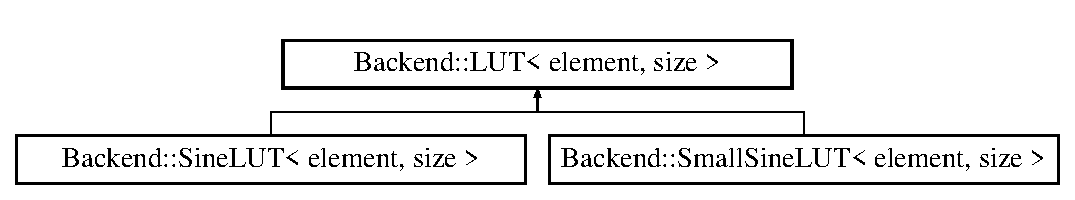
\includegraphics[height=2.000000cm]{classBackend_1_1LUT}
\end{center}
\end{figure}
\subsection*{Public Member Functions}
\begin{DoxyCompactItemize}
\item 
\hyperlink{classBackend_1_1LUT_a8541a1794b0eef2e15eadcfab8cdb12f}{L\+U\+T} ()
\item 
virtual \hyperlink{classBackend_1_1LUT_a1c4d93f58ba28397417f71f436740034}{$\sim$\+L\+U\+T} ()
\item 
element const \& \hyperlink{classBackend_1_1LUT_a9a7c75f36c72778098a091db3269c29c}{operator\mbox{[}$\,$\mbox{]}} (unsigned long const \&index)
\item 
virtual element \hyperlink{classBackend_1_1LUT_aea3420a7a3552f38ba8f9ea979bab764}{operator()} (double const \&x)
\item 
unsigned long const \& \hyperlink{classBackend_1_1LUT_a3ab84f04569e89cd6046da599c6edbae}{Size} () const 
\end{DoxyCompactItemize}
\subsection*{Protected Attributes}
\begin{DoxyCompactItemize}
\item 
element \hyperlink{classBackend_1_1LUT_ae70f3f0c9aaa9e0b85517d8e2c61d9a5}{\+\_\+table} \mbox{[}size\mbox{]}
\item 
const unsigned long \hyperlink{classBackend_1_1LUT_a94d2ce1a7c644ce2d4f8e905790b9b54}{\+\_\+size}
\end{DoxyCompactItemize}


\subsection{Detailed Description}
\subsubsection*{template$<$typename element, unsigned long size$>$class Backend\+::\+L\+U\+T$<$ element, size $>$}



Definition at line 18 of file L\+U\+T.\+h.



\subsection{Constructor \& Destructor Documentation}
\hypertarget{classBackend_1_1LUT_a8541a1794b0eef2e15eadcfab8cdb12f}{\index{Backend\+::\+L\+U\+T@{Backend\+::\+L\+U\+T}!L\+U\+T@{L\+U\+T}}
\index{L\+U\+T@{L\+U\+T}!Backend\+::\+L\+U\+T@{Backend\+::\+L\+U\+T}}
\subsubsection[{L\+U\+T}]{\setlength{\rightskip}{0pt plus 5cm}template$<$typename element, unsigned long size$>$ {\bf Backend\+::\+L\+U\+T}$<$ element, size $>$\+::{\bf L\+U\+T} (
\begin{DoxyParamCaption}
{}
\end{DoxyParamCaption}
)\hspace{0.3cm}{\ttfamily [inline]}}}\label{classBackend_1_1LUT_a8541a1794b0eef2e15eadcfab8cdb12f}


Definition at line 20 of file L\+U\+T.\+h.


\begin{DoxyCode}
20 :\hyperlink{classBackend_1_1LUT_a94d2ce1a7c644ce2d4f8e905790b9b54}{\_size}(size)\{\}
\end{DoxyCode}
\hypertarget{classBackend_1_1LUT_a1c4d93f58ba28397417f71f436740034}{\index{Backend\+::\+L\+U\+T@{Backend\+::\+L\+U\+T}!````~L\+U\+T@{$\sim$\+L\+U\+T}}
\index{````~L\+U\+T@{$\sim$\+L\+U\+T}!Backend\+::\+L\+U\+T@{Backend\+::\+L\+U\+T}}
\subsubsection[{$\sim$\+L\+U\+T}]{\setlength{\rightskip}{0pt plus 5cm}template$<$typename element, unsigned long size$>$ virtual {\bf Backend\+::\+L\+U\+T}$<$ element, size $>$\+::$\sim${\bf L\+U\+T} (
\begin{DoxyParamCaption}
{}
\end{DoxyParamCaption}
)\hspace{0.3cm}{\ttfamily [inline]}, {\ttfamily [virtual]}}}\label{classBackend_1_1LUT_a1c4d93f58ba28397417f71f436740034}


Definition at line 21 of file L\+U\+T.\+h.


\begin{DoxyCode}
21 \{\}
\end{DoxyCode}


\subsection{Member Function Documentation}
\hypertarget{classBackend_1_1LUT_aea3420a7a3552f38ba8f9ea979bab764}{\index{Backend\+::\+L\+U\+T@{Backend\+::\+L\+U\+T}!operator()@{operator()}}
\index{operator()@{operator()}!Backend\+::\+L\+U\+T@{Backend\+::\+L\+U\+T}}
\subsubsection[{operator()}]{\setlength{\rightskip}{0pt plus 5cm}template$<$typename element, unsigned long size$>$ virtual element {\bf Backend\+::\+L\+U\+T}$<$ element, size $>$\+::operator() (
\begin{DoxyParamCaption}
\item[{double const \&}]{x}
\end{DoxyParamCaption}
)\hspace{0.3cm}{\ttfamily [inline]}, {\ttfamily [virtual]}}}\label{classBackend_1_1LUT_aea3420a7a3552f38ba8f9ea979bab764}


Reimplemented in \hyperlink{classBackend_1_1SmallSineLUT_3_01int32__t_00_01size_01_4_a7eff39a75385950b722ed2ba7140d4e4}{Backend\+::\+Small\+Sine\+L\+U\+T$<$ int32\+\_\+t, size $>$}, \hyperlink{classBackend_1_1SmallSineLUT_a2b6fdef4f825da7555ca4002f1dd94af}{Backend\+::\+Small\+Sine\+L\+U\+T$<$ element, size $>$}, and \hyperlink{classBackend_1_1SineLUT_a461395dab282ae8ac9b517caf2d6a553}{Backend\+::\+Sine\+L\+U\+T$<$ element, size $>$}.



Definition at line 28 of file L\+U\+T.\+h.


\begin{DoxyCode}
28                                                            \{
29             \textcolor{keywordflow}{return} 0;
30         \}
\end{DoxyCode}
\hypertarget{classBackend_1_1LUT_a9a7c75f36c72778098a091db3269c29c}{\index{Backend\+::\+L\+U\+T@{Backend\+::\+L\+U\+T}!operator\mbox{[}$\,$\mbox{]}@{operator[]}}
\index{operator\mbox{[}$\,$\mbox{]}@{operator[]}!Backend\+::\+L\+U\+T@{Backend\+::\+L\+U\+T}}
\subsubsection[{operator[]}]{\setlength{\rightskip}{0pt plus 5cm}template$<$typename element, unsigned long size$>$ element const\& {\bf Backend\+::\+L\+U\+T}$<$ element, size $>$\+::operator\mbox{[}$\,$\mbox{]} (
\begin{DoxyParamCaption}
\item[{unsigned long const \&}]{index}
\end{DoxyParamCaption}
)\hspace{0.3cm}{\ttfamily [inline]}}}\label{classBackend_1_1LUT_a9a7c75f36c72778098a091db3269c29c}


Definition at line 22 of file L\+U\+T.\+h.


\begin{DoxyCode}
22                                                              \{
23 \textcolor{preprocessor}{#ifdef DEBUG}
24             assert(index<\hyperlink{classBackend_1_1LUT_a94d2ce1a7c644ce2d4f8e905790b9b54}{\_size});
25 \textcolor{preprocessor}{#endif}
26             \textcolor{keywordflow}{return} \hyperlink{classBackend_1_1LUT_ae70f3f0c9aaa9e0b85517d8e2c61d9a5}{\_table}[index];
27         \}
\end{DoxyCode}
\hypertarget{classBackend_1_1LUT_a3ab84f04569e89cd6046da599c6edbae}{\index{Backend\+::\+L\+U\+T@{Backend\+::\+L\+U\+T}!Size@{Size}}
\index{Size@{Size}!Backend\+::\+L\+U\+T@{Backend\+::\+L\+U\+T}}
\subsubsection[{Size}]{\setlength{\rightskip}{0pt plus 5cm}template$<$typename element, unsigned long size$>$ unsigned long const\& {\bf Backend\+::\+L\+U\+T}$<$ element, size $>$\+::Size (
\begin{DoxyParamCaption}
{}
\end{DoxyParamCaption}
) const\hspace{0.3cm}{\ttfamily [inline]}}}\label{classBackend_1_1LUT_a3ab84f04569e89cd6046da599c6edbae}


Definition at line 31 of file L\+U\+T.\+h.


\begin{DoxyCode}
31                                         \{
32             \textcolor{keywordflow}{return} \hyperlink{classBackend_1_1LUT_a94d2ce1a7c644ce2d4f8e905790b9b54}{\_size};
33         \}
\end{DoxyCode}


\subsection{Member Data Documentation}
\hypertarget{classBackend_1_1LUT_a94d2ce1a7c644ce2d4f8e905790b9b54}{\index{Backend\+::\+L\+U\+T@{Backend\+::\+L\+U\+T}!\+\_\+size@{\+\_\+size}}
\index{\+\_\+size@{\+\_\+size}!Backend\+::\+L\+U\+T@{Backend\+::\+L\+U\+T}}
\subsubsection[{\+\_\+size}]{\setlength{\rightskip}{0pt plus 5cm}template$<$typename element, unsigned long size$>$ const unsigned long {\bf Backend\+::\+L\+U\+T}$<$ element, size $>$\+::\+\_\+size\hspace{0.3cm}{\ttfamily [protected]}}}\label{classBackend_1_1LUT_a94d2ce1a7c644ce2d4f8e905790b9b54}


Definition at line 36 of file L\+U\+T.\+h.

\hypertarget{classBackend_1_1LUT_ae70f3f0c9aaa9e0b85517d8e2c61d9a5}{\index{Backend\+::\+L\+U\+T@{Backend\+::\+L\+U\+T}!\+\_\+table@{\+\_\+table}}
\index{\+\_\+table@{\+\_\+table}!Backend\+::\+L\+U\+T@{Backend\+::\+L\+U\+T}}
\subsubsection[{\+\_\+table}]{\setlength{\rightskip}{0pt plus 5cm}template$<$typename element, unsigned long size$>$ element {\bf Backend\+::\+L\+U\+T}$<$ element, size $>$\+::\+\_\+table\mbox{[}size\mbox{]}\hspace{0.3cm}{\ttfamily [protected]}}}\label{classBackend_1_1LUT_ae70f3f0c9aaa9e0b85517d8e2c61d9a5}


Definition at line 35 of file L\+U\+T.\+h.



The documentation for this class was generated from the following file\+:\begin{DoxyCompactItemize}
\item 
/\+Users/alexanderzywicki/\+Documents/\+School\+\_\+\+Stuff/\+Fall\+\_\+2014/\+Digital\+\_\+\+Signal\+\_\+\+Generation\+\_\+and\+\_\+\+Analysis/src/include/\hyperlink{LUT_8h}{L\+U\+T.\+h}\end{DoxyCompactItemize}

\hypertarget{classSignal_1_1BLEP_1_1minBLEP}{\section{Signal\+:\+:B\+L\+E\+P\+:\+:min\+B\+L\+E\+P Class Reference}
\label{classSignal_1_1BLEP_1_1minBLEP}\index{Signal\+::\+B\+L\+E\+P\+::min\+B\+L\+E\+P@{Signal\+::\+B\+L\+E\+P\+::min\+B\+L\+E\+P}}
}


{\ttfamily \#include $<$min\+B\+L\+E\+P.\+h$>$}

Inheritance diagram for Signal\+:\+:B\+L\+E\+P\+:\+:min\+B\+L\+E\+P\+:\begin{figure}[H]
\begin{center}
\leavevmode
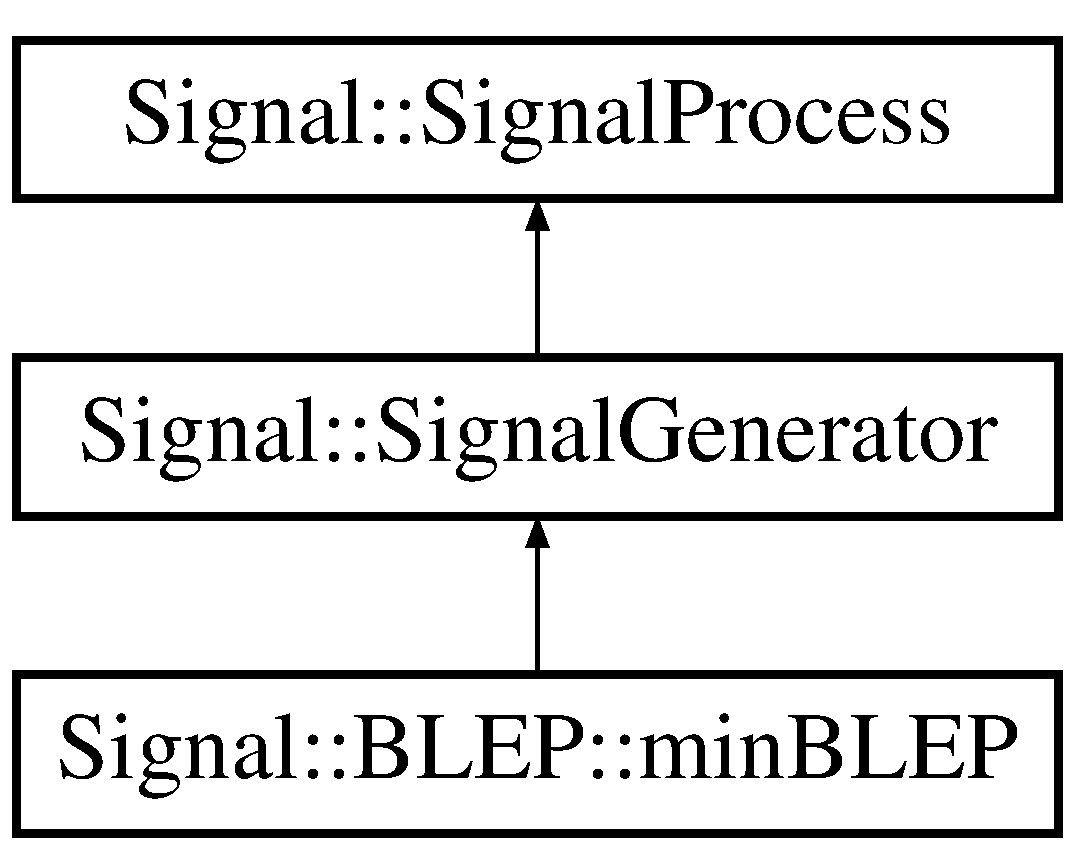
\includegraphics[height=3.000000cm]{classSignal_1_1BLEP_1_1minBLEP}
\end{center}
\end{figure}
\subsection*{Public Member Functions}
\begin{DoxyCompactItemize}
\item 
virtual bool \hyperlink{classSignal_1_1SignalGenerator_a2cd9061c5ae40a392a9476551b4379f3}{Perform} (\hyperlink{classSignal_1_1Sample}{Sample} \&signal)
\item 
virtual bool \hyperlink{classSignal_1_1SignalGenerator_a126d52dd9b6b14d33efc624e2c89284e}{Perform} (\hyperlink{classSignal_1_1RingBuffer}{Ring\+Buffer} \&signal)
\item 
virtual double const \& \hyperlink{classSignal_1_1SignalGenerator_a96af42ee68f94e9b04d034fd68b73ecd}{Frequency} () const 
\item 
virtual double const \& \hyperlink{classSignal_1_1SignalGenerator_af83b532bf3ddc3637c2fd7a1dfd095cb}{Frequency} (double const \&value)
\item 
virtual double const \& \hyperlink{classSignal_1_1SignalGenerator_ac2538ec946f001e394d2416fda698d1c}{Phase\+Offset} () const 
\item 
virtual double const \& \hyperlink{classSignal_1_1SignalGenerator_ac6a103ff72beaa338f6d18c812522d78}{Phase\+Offset} (double const \&value)
\end{DoxyCompactItemize}
\subsection*{Protected Attributes}
\begin{DoxyCompactItemize}
\item 
double \hyperlink{classSignal_1_1SignalGenerator_a7f107461333bce68c5dad412db96a8c2}{\+\_\+frequency}
\item 
double \hyperlink{classSignal_1_1SignalGenerator_a85a4702347352bab1c71e0a8df8437d6}{\+\_\+f\+Hertz}
\item 
double \hyperlink{classSignal_1_1SignalGenerator_a6b4444d46747c8517171edbbf4b5588f}{\+\_\+phase\+\_\+offset}
\end{DoxyCompactItemize}


\subsection{Detailed Description}


Definition at line 16 of file min\+B\+L\+E\+P.\+h.



\subsection{Member Function Documentation}
\hypertarget{classSignal_1_1SignalGenerator_a96af42ee68f94e9b04d034fd68b73ecd}{\index{Signal\+::\+B\+L\+E\+P\+::min\+B\+L\+E\+P@{Signal\+::\+B\+L\+E\+P\+::min\+B\+L\+E\+P}!Frequency@{Frequency}}
\index{Frequency@{Frequency}!Signal\+::\+B\+L\+E\+P\+::min\+B\+L\+E\+P@{Signal\+::\+B\+L\+E\+P\+::min\+B\+L\+E\+P}}
\subsubsection[{Frequency}]{\setlength{\rightskip}{0pt plus 5cm}double const \& Signal\+::\+Signal\+Generator\+::\+Frequency (
\begin{DoxyParamCaption}
{}
\end{DoxyParamCaption}
) const\hspace{0.3cm}{\ttfamily [virtual]}, {\ttfamily [inherited]}}}\label{classSignal_1_1SignalGenerator_a96af42ee68f94e9b04d034fd68b73ecd}


Definition at line 16 of file Signal\+Generator.\+cpp.


\begin{DoxyCode}
16                                                    \{
17     \textcolor{keywordflow}{return} \hyperlink{classSignal_1_1SignalGenerator_a85a4702347352bab1c71e0a8df8437d6}{\_fHertz};
18 \}
\end{DoxyCode}
\hypertarget{classSignal_1_1SignalGenerator_af83b532bf3ddc3637c2fd7a1dfd095cb}{\index{Signal\+::\+B\+L\+E\+P\+::min\+B\+L\+E\+P@{Signal\+::\+B\+L\+E\+P\+::min\+B\+L\+E\+P}!Frequency@{Frequency}}
\index{Frequency@{Frequency}!Signal\+::\+B\+L\+E\+P\+::min\+B\+L\+E\+P@{Signal\+::\+B\+L\+E\+P\+::min\+B\+L\+E\+P}}
\subsubsection[{Frequency}]{\setlength{\rightskip}{0pt plus 5cm}double const \& Signal\+::\+Signal\+Generator\+::\+Frequency (
\begin{DoxyParamCaption}
\item[{double const \&}]{value}
\end{DoxyParamCaption}
)\hspace{0.3cm}{\ttfamily [virtual]}, {\ttfamily [inherited]}}}\label{classSignal_1_1SignalGenerator_af83b532bf3ddc3637c2fd7a1dfd095cb}


Reimplemented in \hyperlink{classSignal_1_1BLIT_1_1BLIT_a59110620478308054d4c932c613e5cc6}{Signal\+::\+B\+L\+I\+T\+::\+B\+L\+I\+T}, \hyperlink{classSignal_1_1Fourier_1_1Saw_a398a26142f42cdc5cb33230e9ab05b9d}{Signal\+::\+Fourier\+::\+Saw}, and \hyperlink{classSignal_1_1Fourier_1_1Square_a99040022c5d7c9f88e52cdeeed3e797a}{Signal\+::\+Fourier\+::\+Square}.



Definition at line 19 of file Signal\+Generator.\+cpp.


\begin{DoxyCode}
19                                                                  \{
20     \hyperlink{classSignal_1_1SignalGenerator_a85a4702347352bab1c71e0a8df8437d6}{\_fHertz} = value;
21     \hyperlink{classSignal_1_1SignalGenerator_a7f107461333bce68c5dad412db96a8c2}{\_frequency} = \hyperlink{classSignal_1_1SignalGenerator_a85a4702347352bab1c71e0a8df8437d6}{\_fHertz}/\hyperlink{namespaceSignal_ae7b1f222afc010e0f33f306f978fcde9}{Sample\_Rate}();
22     \textcolor{keywordflow}{return} \hyperlink{classSignal_1_1SignalGenerator_a85a4702347352bab1c71e0a8df8437d6}{\_fHertz};
23 \}
\end{DoxyCode}
\hypertarget{classSignal_1_1SignalGenerator_a2cd9061c5ae40a392a9476551b4379f3}{\index{Signal\+::\+B\+L\+E\+P\+::min\+B\+L\+E\+P@{Signal\+::\+B\+L\+E\+P\+::min\+B\+L\+E\+P}!Perform@{Perform}}
\index{Perform@{Perform}!Signal\+::\+B\+L\+E\+P\+::min\+B\+L\+E\+P@{Signal\+::\+B\+L\+E\+P\+::min\+B\+L\+E\+P}}
\subsubsection[{Perform}]{\setlength{\rightskip}{0pt plus 5cm}bool Signal\+::\+Signal\+Generator\+::\+Perform (
\begin{DoxyParamCaption}
\item[{{\bf Sample} \&}]{signal}
\end{DoxyParamCaption}
)\hspace{0.3cm}{\ttfamily [inline]}, {\ttfamily [virtual]}, {\ttfamily [inherited]}}}\label{classSignal_1_1SignalGenerator_a2cd9061c5ae40a392a9476551b4379f3}


Implements \hyperlink{classSignal_1_1SignalProcess_a7986df989ac8afca3674ae8eace3cfdb}{Signal\+::\+Signal\+Process}.



Reimplemented in \hyperlink{classSignal_1_1Fourier_1_1Sine_aa35c77904f8d7a0de6fa4895d6c53644}{Signal\+::\+Fourier\+::\+Sine}, \hyperlink{classSignal_1_1Fourier_1_1FourierGenerator_a6ec444e7b66d2cb339c001704071646a}{Signal\+::\+Fourier\+::\+Fourier\+Generator}, \hyperlink{classSignal_1_1BLIT_1_1BLIT_a98982b34bc6c9ca4c2e91550afa31375}{Signal\+::\+B\+L\+I\+T\+::\+B\+L\+I\+T}, \hyperlink{classSignal_1_1Trivial_1_1TrivialGenerator_a2394cf9d0d40f9d25f72aff03e372ad9}{Signal\+::\+Trivial\+::\+Trivial\+Generator}, \hyperlink{classSignal_1_1Fourier_1_1Saw_adf69eea95516fc9c7d06fae036d2fa9b}{Signal\+::\+Fourier\+::\+Saw}, \hyperlink{classSignal_1_1Fourier_1_1Square_a29e4b9d03b9df4fb6ed0d7a817ecffda}{Signal\+::\+Fourier\+::\+Square}, and \hyperlink{classSignal_1_1Trivial_1_1TrivialSaw_a091e3137a03978cc7dfaecf5b00dad46}{Signal\+::\+Trivial\+::\+Trivial\+Saw}.



Definition at line 39 of file Signal\+Generator.\+h.


\begin{DoxyCode}
39                                                       \{
40         signal = 0;
41         \textcolor{keywordflow}{return} \textcolor{keyword}{false};
42     \}
\end{DoxyCode}
\hypertarget{classSignal_1_1SignalGenerator_a126d52dd9b6b14d33efc624e2c89284e}{\index{Signal\+::\+B\+L\+E\+P\+::min\+B\+L\+E\+P@{Signal\+::\+B\+L\+E\+P\+::min\+B\+L\+E\+P}!Perform@{Perform}}
\index{Perform@{Perform}!Signal\+::\+B\+L\+E\+P\+::min\+B\+L\+E\+P@{Signal\+::\+B\+L\+E\+P\+::min\+B\+L\+E\+P}}
\subsubsection[{Perform}]{\setlength{\rightskip}{0pt plus 5cm}bool Signal\+::\+Signal\+Generator\+::\+Perform (
\begin{DoxyParamCaption}
\item[{{\bf Ring\+Buffer} \&}]{signal}
\end{DoxyParamCaption}
)\hspace{0.3cm}{\ttfamily [inline]}, {\ttfamily [virtual]}, {\ttfamily [inherited]}}}\label{classSignal_1_1SignalGenerator_a126d52dd9b6b14d33efc624e2c89284e}


Implements \hyperlink{classSignal_1_1SignalProcess_a9584dc515d2167f4439ed3d014bbb3f7}{Signal\+::\+Signal\+Process}.



Reimplemented in \hyperlink{classSignal_1_1Fourier_1_1Sine_a5d951e5fbfc77354bddab9dfedea008f}{Signal\+::\+Fourier\+::\+Sine}, \hyperlink{classSignal_1_1Fourier_1_1FourierGenerator_acc6a3825eb4060269749a37ae29ee847}{Signal\+::\+Fourier\+::\+Fourier\+Generator}, \hyperlink{classSignal_1_1BLIT_1_1BLIT_a2f0ee604ed0e67557aa9f7e7f50d80ec}{Signal\+::\+B\+L\+I\+T\+::\+B\+L\+I\+T}, \hyperlink{classSignal_1_1Trivial_1_1TrivialGenerator_a232aefbb2815eaf25e697ecedeb0f3d9}{Signal\+::\+Trivial\+::\+Trivial\+Generator}, \hyperlink{classSignal_1_1Fourier_1_1Saw_acef099db2217902d7157e5b93f658363}{Signal\+::\+Fourier\+::\+Saw}, \hyperlink{classSignal_1_1Fourier_1_1Square_a7aacafda4427b996b56ad6764ea09177}{Signal\+::\+Fourier\+::\+Square}, and \hyperlink{classSignal_1_1Trivial_1_1TrivialSaw_a22b97c8dfdca76664cbb6e634c85085d}{Signal\+::\+Trivial\+::\+Trivial\+Saw}.



Definition at line 43 of file Signal\+Generator.\+h.


\begin{DoxyCode}
43                                                           \{
44         signal.Flush();
45         \textcolor{keywordflow}{return} \textcolor{keyword}{false};
46     \}
\end{DoxyCode}
\hypertarget{classSignal_1_1SignalGenerator_ac2538ec946f001e394d2416fda698d1c}{\index{Signal\+::\+B\+L\+E\+P\+::min\+B\+L\+E\+P@{Signal\+::\+B\+L\+E\+P\+::min\+B\+L\+E\+P}!Phase\+Offset@{Phase\+Offset}}
\index{Phase\+Offset@{Phase\+Offset}!Signal\+::\+B\+L\+E\+P\+::min\+B\+L\+E\+P@{Signal\+::\+B\+L\+E\+P\+::min\+B\+L\+E\+P}}
\subsubsection[{Phase\+Offset}]{\setlength{\rightskip}{0pt plus 5cm}double const \& Signal\+::\+Signal\+Generator\+::\+Phase\+Offset (
\begin{DoxyParamCaption}
{}
\end{DoxyParamCaption}
) const\hspace{0.3cm}{\ttfamily [virtual]}, {\ttfamily [inherited]}}}\label{classSignal_1_1SignalGenerator_ac2538ec946f001e394d2416fda698d1c}


Definition at line 24 of file Signal\+Generator.\+cpp.


\begin{DoxyCode}
24                                                      \{
25     \textcolor{keywordflow}{return} \hyperlink{classSignal_1_1SignalGenerator_a6b4444d46747c8517171edbbf4b5588f}{\_phase\_offset};
26 \}
\end{DoxyCode}
\hypertarget{classSignal_1_1SignalGenerator_ac6a103ff72beaa338f6d18c812522d78}{\index{Signal\+::\+B\+L\+E\+P\+::min\+B\+L\+E\+P@{Signal\+::\+B\+L\+E\+P\+::min\+B\+L\+E\+P}!Phase\+Offset@{Phase\+Offset}}
\index{Phase\+Offset@{Phase\+Offset}!Signal\+::\+B\+L\+E\+P\+::min\+B\+L\+E\+P@{Signal\+::\+B\+L\+E\+P\+::min\+B\+L\+E\+P}}
\subsubsection[{Phase\+Offset}]{\setlength{\rightskip}{0pt plus 5cm}double const \& Signal\+::\+Signal\+Generator\+::\+Phase\+Offset (
\begin{DoxyParamCaption}
\item[{double const \&}]{value}
\end{DoxyParamCaption}
)\hspace{0.3cm}{\ttfamily [virtual]}, {\ttfamily [inherited]}}}\label{classSignal_1_1SignalGenerator_ac6a103ff72beaa338f6d18c812522d78}


Definition at line 27 of file Signal\+Generator.\+cpp.


\begin{DoxyCode}
27                                                                    \{
28     \hyperlink{classSignal_1_1SignalGenerator_a6b4444d46747c8517171edbbf4b5588f}{\_phase\_offset} = value;
29     \textcolor{keywordflow}{return} \hyperlink{classSignal_1_1SignalGenerator_a6b4444d46747c8517171edbbf4b5588f}{\_phase\_offset};
30 \}
\end{DoxyCode}


\subsection{Member Data Documentation}
\hypertarget{classSignal_1_1SignalGenerator_a85a4702347352bab1c71e0a8df8437d6}{\index{Signal\+::\+B\+L\+E\+P\+::min\+B\+L\+E\+P@{Signal\+::\+B\+L\+E\+P\+::min\+B\+L\+E\+P}!\+\_\+f\+Hertz@{\+\_\+f\+Hertz}}
\index{\+\_\+f\+Hertz@{\+\_\+f\+Hertz}!Signal\+::\+B\+L\+E\+P\+::min\+B\+L\+E\+P@{Signal\+::\+B\+L\+E\+P\+::min\+B\+L\+E\+P}}
\subsubsection[{\+\_\+f\+Hertz}]{\setlength{\rightskip}{0pt plus 5cm}double Signal\+::\+Signal\+Generator\+::\+\_\+f\+Hertz\hspace{0.3cm}{\ttfamily [protected]}, {\ttfamily [inherited]}}}\label{classSignal_1_1SignalGenerator_a85a4702347352bab1c71e0a8df8437d6}


Definition at line 34 of file Signal\+Generator.\+h.

\hypertarget{classSignal_1_1SignalGenerator_a7f107461333bce68c5dad412db96a8c2}{\index{Signal\+::\+B\+L\+E\+P\+::min\+B\+L\+E\+P@{Signal\+::\+B\+L\+E\+P\+::min\+B\+L\+E\+P}!\+\_\+frequency@{\+\_\+frequency}}
\index{\+\_\+frequency@{\+\_\+frequency}!Signal\+::\+B\+L\+E\+P\+::min\+B\+L\+E\+P@{Signal\+::\+B\+L\+E\+P\+::min\+B\+L\+E\+P}}
\subsubsection[{\+\_\+frequency}]{\setlength{\rightskip}{0pt plus 5cm}double Signal\+::\+Signal\+Generator\+::\+\_\+frequency\hspace{0.3cm}{\ttfamily [protected]}, {\ttfamily [inherited]}}}\label{classSignal_1_1SignalGenerator_a7f107461333bce68c5dad412db96a8c2}


Definition at line 33 of file Signal\+Generator.\+h.

\hypertarget{classSignal_1_1SignalGenerator_a6b4444d46747c8517171edbbf4b5588f}{\index{Signal\+::\+B\+L\+E\+P\+::min\+B\+L\+E\+P@{Signal\+::\+B\+L\+E\+P\+::min\+B\+L\+E\+P}!\+\_\+phase\+\_\+offset@{\+\_\+phase\+\_\+offset}}
\index{\+\_\+phase\+\_\+offset@{\+\_\+phase\+\_\+offset}!Signal\+::\+B\+L\+E\+P\+::min\+B\+L\+E\+P@{Signal\+::\+B\+L\+E\+P\+::min\+B\+L\+E\+P}}
\subsubsection[{\+\_\+phase\+\_\+offset}]{\setlength{\rightskip}{0pt plus 5cm}double Signal\+::\+Signal\+Generator\+::\+\_\+phase\+\_\+offset\hspace{0.3cm}{\ttfamily [protected]}, {\ttfamily [inherited]}}}\label{classSignal_1_1SignalGenerator_a6b4444d46747c8517171edbbf4b5588f}


Definition at line 35 of file Signal\+Generator.\+h.



The documentation for this class was generated from the following file\+:\begin{DoxyCompactItemize}
\item 
/\+Users/alexanderzywicki/\+Documents/\+School\+\_\+\+Stuff/\+Fall\+\_\+2014/\+Digital\+\_\+\+Signal\+\_\+\+Generation\+\_\+and\+\_\+\+Analysis/src/include/\hyperlink{minBLEP_8h}{min\+B\+L\+E\+P.\+h}\end{DoxyCompactItemize}

\hypertarget{classSignal_1_1BLEP_1_1polyBLEP}{\section{Signal\+:\+:B\+L\+E\+P\+:\+:poly\+B\+L\+E\+P Class Reference}
\label{classSignal_1_1BLEP_1_1polyBLEP}\index{Signal\+::\+B\+L\+E\+P\+::poly\+B\+L\+E\+P@{Signal\+::\+B\+L\+E\+P\+::poly\+B\+L\+E\+P}}
}


See file $\sim$/\+Research/poly\+B\+L\+E\+P.rtf for links to deatils about algorithm.  




{\ttfamily \#include $<$poly\+B\+L\+E\+P.\+h$>$}

Inheritance diagram for Signal\+:\+:B\+L\+E\+P\+:\+:poly\+B\+L\+E\+P\+:\begin{figure}[H]
\begin{center}
\leavevmode
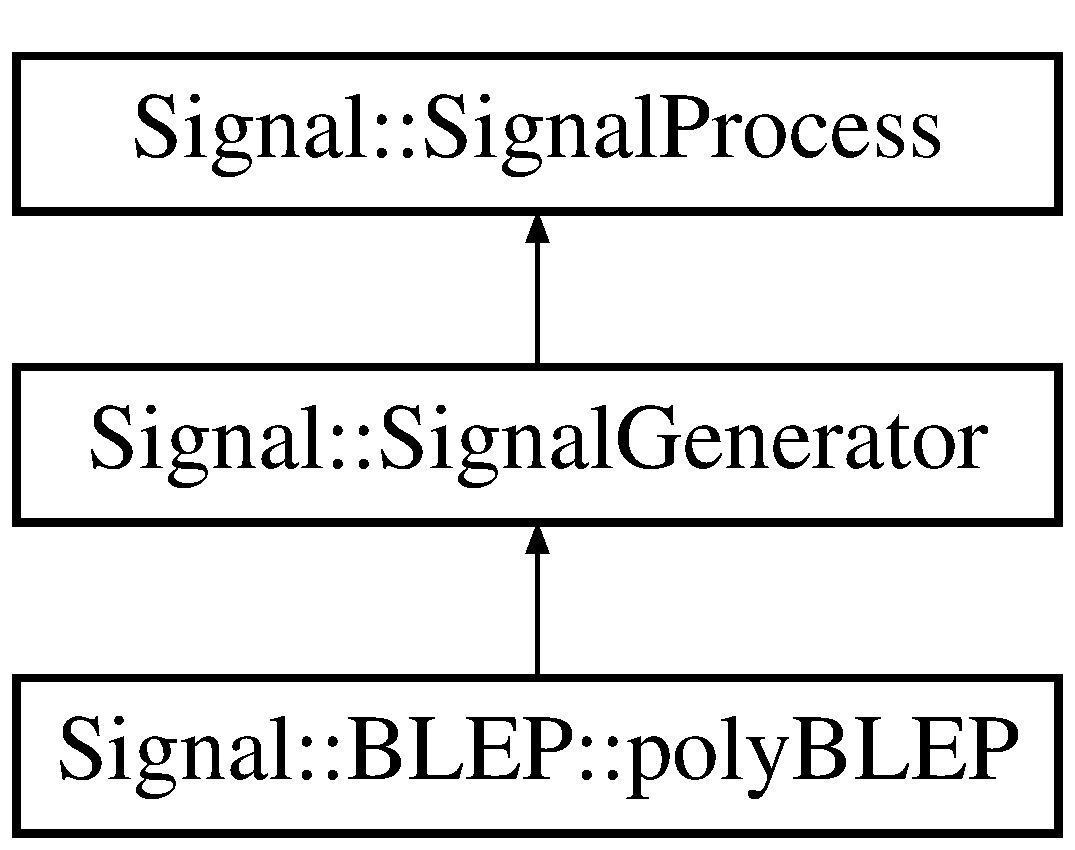
\includegraphics[height=3.000000cm]{classSignal_1_1BLEP_1_1polyBLEP}
\end{center}
\end{figure}
\subsection*{Public Member Functions}
\begin{DoxyCompactItemize}
\item 
virtual bool \hyperlink{classSignal_1_1SignalGenerator_a2cd9061c5ae40a392a9476551b4379f3}{Perform} (\hyperlink{classSignal_1_1Sample}{Sample} \&signal)
\item 
virtual bool \hyperlink{classSignal_1_1SignalGenerator_a126d52dd9b6b14d33efc624e2c89284e}{Perform} (\hyperlink{classSignal_1_1RingBuffer}{Ring\+Buffer} \&signal)
\item 
virtual double const \& \hyperlink{classSignal_1_1SignalGenerator_a96af42ee68f94e9b04d034fd68b73ecd}{Frequency} () const 
\item 
virtual double const \& \hyperlink{classSignal_1_1SignalGenerator_af83b532bf3ddc3637c2fd7a1dfd095cb}{Frequency} (double const \&value)
\item 
virtual double const \& \hyperlink{classSignal_1_1SignalGenerator_ac2538ec946f001e394d2416fda698d1c}{Phase\+Offset} () const 
\item 
virtual double const \& \hyperlink{classSignal_1_1SignalGenerator_ac6a103ff72beaa338f6d18c812522d78}{Phase\+Offset} (double const \&value)
\end{DoxyCompactItemize}
\subsection*{Protected Member Functions}
\begin{DoxyCompactItemize}
\item 
double \hyperlink{classSignal_1_1SignalGenerator_a43b0eec84ee7df04c947533c0511c2c0}{\+\_\+pstep} ()
\item 
double \hyperlink{classSignal_1_1SignalGenerator_abf2f4ab977c6e84bf85022eab8135304}{\+\_\+pstep\+\_\+rad} ()
\item 
void \hyperlink{classSignal_1_1SignalGenerator_a563f57d4dfd8728a6a572f15c1e2532b}{\+\_\+psync} ()
\end{DoxyCompactItemize}
\subsection*{Protected Attributes}
\begin{DoxyCompactItemize}
\item 
double \hyperlink{classSignal_1_1SignalGenerator_a7f107461333bce68c5dad412db96a8c2}{\+\_\+frequency}
\item 
double \hyperlink{classSignal_1_1SignalGenerator_a85a4702347352bab1c71e0a8df8437d6}{\+\_\+f\+Hertz}
\item 
double \hyperlink{classSignal_1_1SignalGenerator_a6b4444d46747c8517171edbbf4b5588f}{\+\_\+phase\+\_\+offset}
\item 
double \hyperlink{classSignal_1_1SignalGenerator_af4aa0728ded00777be26a06d883eaeb3}{\+\_\+phasor}
\end{DoxyCompactItemize}


\subsection{Detailed Description}
See file $\sim$/\+Research/poly\+B\+L\+E\+P.rtf for links to deatils about algorithm. 

Definition at line 20 of file poly\+B\+L\+E\+P.\+h.



\subsection{Member Function Documentation}
\hypertarget{classSignal_1_1SignalGenerator_a43b0eec84ee7df04c947533c0511c2c0}{\index{Signal\+::\+B\+L\+E\+P\+::poly\+B\+L\+E\+P@{Signal\+::\+B\+L\+E\+P\+::poly\+B\+L\+E\+P}!\+\_\+pstep@{\+\_\+pstep}}
\index{\+\_\+pstep@{\+\_\+pstep}!Signal\+::\+B\+L\+E\+P\+::poly\+B\+L\+E\+P@{Signal\+::\+B\+L\+E\+P\+::poly\+B\+L\+E\+P}}
\subsubsection[{\+\_\+pstep}]{\setlength{\rightskip}{0pt plus 5cm}double Signal\+::\+Signal\+Generator\+::\+\_\+pstep (
\begin{DoxyParamCaption}
{}
\end{DoxyParamCaption}
)\hspace{0.3cm}{\ttfamily [inline]}, {\ttfamily [protected]}, {\ttfamily [inherited]}}}\label{classSignal_1_1SignalGenerator_a43b0eec84ee7df04c947533c0511c2c0}


Definition at line 59 of file Signal\+Generator.\+h.


\begin{DoxyCode}
59                                          \{
60         \textcolor{keywordtype}{double} value = \hyperlink{classSignal_1_1SignalGenerator_af4aa0728ded00777be26a06d883eaeb3}{\_phasor};
61         \hyperlink{classSignal_1_1SignalGenerator_af4aa0728ded00777be26a06d883eaeb3}{\_phasor}+=\hyperlink{classSignal_1_1SignalGenerator_a7f107461333bce68c5dad412db96a8c2}{\_frequency};
62         \hyperlink{classSignal_1_1SignalGenerator_af4aa0728ded00777be26a06d883eaeb3}{\_phasor} = \hyperlink{classSignal_1_1SignalGenerator_af4aa0728ded00777be26a06d883eaeb3}{\_phasor}-(\textcolor{keywordtype}{unsigned} long)\hyperlink{classSignal_1_1SignalGenerator_af4aa0728ded00777be26a06d883eaeb3}{\_phasor};\textcolor{comment}{//cheaper %1}
63         \textcolor{keywordflow}{return} value;
64     \}
\end{DoxyCode}
\hypertarget{classSignal_1_1SignalGenerator_abf2f4ab977c6e84bf85022eab8135304}{\index{Signal\+::\+B\+L\+E\+P\+::poly\+B\+L\+E\+P@{Signal\+::\+B\+L\+E\+P\+::poly\+B\+L\+E\+P}!\+\_\+pstep\+\_\+rad@{\+\_\+pstep\+\_\+rad}}
\index{\+\_\+pstep\+\_\+rad@{\+\_\+pstep\+\_\+rad}!Signal\+::\+B\+L\+E\+P\+::poly\+B\+L\+E\+P@{Signal\+::\+B\+L\+E\+P\+::poly\+B\+L\+E\+P}}
\subsubsection[{\+\_\+pstep\+\_\+rad}]{\setlength{\rightskip}{0pt plus 5cm}double Signal\+::\+Signal\+Generator\+::\+\_\+pstep\+\_\+rad (
\begin{DoxyParamCaption}
{}
\end{DoxyParamCaption}
)\hspace{0.3cm}{\ttfamily [inline]}, {\ttfamily [protected]}, {\ttfamily [inherited]}}}\label{classSignal_1_1SignalGenerator_abf2f4ab977c6e84bf85022eab8135304}


Definition at line 65 of file Signal\+Generator.\+h.


\begin{DoxyCode}
65                                              \{
66         \textcolor{keywordflow}{return} \hyperlink{PI_8h_a4912c64aec0c943b7985db6cb61ff83a}{TWOPI} * \hyperlink{classSignal_1_1SignalGenerator_a43b0eec84ee7df04c947533c0511c2c0}{\_pstep}();
67     \}
\end{DoxyCode}
\hypertarget{classSignal_1_1SignalGenerator_a563f57d4dfd8728a6a572f15c1e2532b}{\index{Signal\+::\+B\+L\+E\+P\+::poly\+B\+L\+E\+P@{Signal\+::\+B\+L\+E\+P\+::poly\+B\+L\+E\+P}!\+\_\+psync@{\+\_\+psync}}
\index{\+\_\+psync@{\+\_\+psync}!Signal\+::\+B\+L\+E\+P\+::poly\+B\+L\+E\+P@{Signal\+::\+B\+L\+E\+P\+::poly\+B\+L\+E\+P}}
\subsubsection[{\+\_\+psync}]{\setlength{\rightskip}{0pt plus 5cm}void Signal\+::\+Signal\+Generator\+::\+\_\+psync (
\begin{DoxyParamCaption}
{}
\end{DoxyParamCaption}
)\hspace{0.3cm}{\ttfamily [inline]}, {\ttfamily [protected]}, {\ttfamily [inherited]}}}\label{classSignal_1_1SignalGenerator_a563f57d4dfd8728a6a572f15c1e2532b}


Definition at line 68 of file Signal\+Generator.\+h.


\begin{DoxyCode}
68                                        \{
69         \hyperlink{classSignal_1_1SignalGenerator_af4aa0728ded00777be26a06d883eaeb3}{\_phasor} = 0;
70     \}
\end{DoxyCode}
\hypertarget{classSignal_1_1SignalGenerator_a96af42ee68f94e9b04d034fd68b73ecd}{\index{Signal\+::\+B\+L\+E\+P\+::poly\+B\+L\+E\+P@{Signal\+::\+B\+L\+E\+P\+::poly\+B\+L\+E\+P}!Frequency@{Frequency}}
\index{Frequency@{Frequency}!Signal\+::\+B\+L\+E\+P\+::poly\+B\+L\+E\+P@{Signal\+::\+B\+L\+E\+P\+::poly\+B\+L\+E\+P}}
\subsubsection[{Frequency}]{\setlength{\rightskip}{0pt plus 5cm}double const \& Signal\+::\+Signal\+Generator\+::\+Frequency (
\begin{DoxyParamCaption}
{}
\end{DoxyParamCaption}
) const\hspace{0.3cm}{\ttfamily [virtual]}, {\ttfamily [inherited]}}}\label{classSignal_1_1SignalGenerator_a96af42ee68f94e9b04d034fd68b73ecd}


Definition at line 16 of file Signal\+Generator.\+cpp.


\begin{DoxyCode}
16                                                    \{
17     \textcolor{keywordflow}{return} \hyperlink{classSignal_1_1SignalGenerator_a85a4702347352bab1c71e0a8df8437d6}{\_fHertz};
18 \}
\end{DoxyCode}
\hypertarget{classSignal_1_1SignalGenerator_af83b532bf3ddc3637c2fd7a1dfd095cb}{\index{Signal\+::\+B\+L\+E\+P\+::poly\+B\+L\+E\+P@{Signal\+::\+B\+L\+E\+P\+::poly\+B\+L\+E\+P}!Frequency@{Frequency}}
\index{Frequency@{Frequency}!Signal\+::\+B\+L\+E\+P\+::poly\+B\+L\+E\+P@{Signal\+::\+B\+L\+E\+P\+::poly\+B\+L\+E\+P}}
\subsubsection[{Frequency}]{\setlength{\rightskip}{0pt plus 5cm}double const \& Signal\+::\+Signal\+Generator\+::\+Frequency (
\begin{DoxyParamCaption}
\item[{double const \&}]{value}
\end{DoxyParamCaption}
)\hspace{0.3cm}{\ttfamily [virtual]}, {\ttfamily [inherited]}}}\label{classSignal_1_1SignalGenerator_af83b532bf3ddc3637c2fd7a1dfd095cb}


Reimplemented in \hyperlink{classSignal_1_1BLIT_1_1BLIT_a59110620478308054d4c932c613e5cc6}{Signal\+::\+B\+L\+I\+T\+::\+B\+L\+I\+T}, \hyperlink{classSignal_1_1Fourier_1_1Saw_a398a26142f42cdc5cb33230e9ab05b9d}{Signal\+::\+Fourier\+::\+Saw}, and \hyperlink{classSignal_1_1Fourier_1_1Square_a99040022c5d7c9f88e52cdeeed3e797a}{Signal\+::\+Fourier\+::\+Square}.



Definition at line 19 of file Signal\+Generator.\+cpp.


\begin{DoxyCode}
19                                                                  \{
20     \hyperlink{classSignal_1_1SignalGenerator_a85a4702347352bab1c71e0a8df8437d6}{\_fHertz} = value;
21     \hyperlink{classSignal_1_1SignalGenerator_a7f107461333bce68c5dad412db96a8c2}{\_frequency} = \hyperlink{classSignal_1_1SignalGenerator_a85a4702347352bab1c71e0a8df8437d6}{\_fHertz}/\hyperlink{namespaceSignal_ae7b1f222afc010e0f33f306f978fcde9}{Sample\_Rate}();
22     \textcolor{keywordflow}{return} \hyperlink{classSignal_1_1SignalGenerator_a85a4702347352bab1c71e0a8df8437d6}{\_fHertz};
23 \}
\end{DoxyCode}
\hypertarget{classSignal_1_1SignalGenerator_a2cd9061c5ae40a392a9476551b4379f3}{\index{Signal\+::\+B\+L\+E\+P\+::poly\+B\+L\+E\+P@{Signal\+::\+B\+L\+E\+P\+::poly\+B\+L\+E\+P}!Perform@{Perform}}
\index{Perform@{Perform}!Signal\+::\+B\+L\+E\+P\+::poly\+B\+L\+E\+P@{Signal\+::\+B\+L\+E\+P\+::poly\+B\+L\+E\+P}}
\subsubsection[{Perform}]{\setlength{\rightskip}{0pt plus 5cm}bool Signal\+::\+Signal\+Generator\+::\+Perform (
\begin{DoxyParamCaption}
\item[{{\bf Sample} \&}]{signal}
\end{DoxyParamCaption}
)\hspace{0.3cm}{\ttfamily [inline]}, {\ttfamily [virtual]}, {\ttfamily [inherited]}}}\label{classSignal_1_1SignalGenerator_a2cd9061c5ae40a392a9476551b4379f3}


Implements \hyperlink{classSignal_1_1SignalProcess_a7986df989ac8afca3674ae8eace3cfdb}{Signal\+::\+Signal\+Process}.



Reimplemented in \hyperlink{classSignal_1_1Fourier_1_1Sine_aa35c77904f8d7a0de6fa4895d6c53644}{Signal\+::\+Fourier\+::\+Sine}, \hyperlink{classSignal_1_1Fourier_1_1FourierGenerator_a6ec444e7b66d2cb339c001704071646a}{Signal\+::\+Fourier\+::\+Fourier\+Generator}, \hyperlink{classSignal_1_1BLIT_1_1BLIT_a98982b34bc6c9ca4c2e91550afa31375}{Signal\+::\+B\+L\+I\+T\+::\+B\+L\+I\+T}, \hyperlink{classSignal_1_1Analog_1_1AnalogGenerator_a435d695634a52cff8249dde68be18e8a}{Signal\+::\+Analog\+::\+Analog\+Generator}, \hyperlink{classSignal_1_1Fourier_1_1Saw_adf69eea95516fc9c7d06fae036d2fa9b}{Signal\+::\+Fourier\+::\+Saw}, \hyperlink{classSignal_1_1Fourier_1_1Square_a29e4b9d03b9df4fb6ed0d7a817ecffda}{Signal\+::\+Fourier\+::\+Square}, \hyperlink{classSignal_1_1Analog_1_1Saw_ac91789b8322a0b39a15bc8dc6506d60b}{Signal\+::\+Analog\+::\+Saw}, and \hyperlink{classSignal_1_1Analog_1_1Square_a4afb9704efebdab680094fad82876357}{Signal\+::\+Analog\+::\+Square}.



Definition at line 51 of file Signal\+Generator.\+h.


\begin{DoxyCode}
51                                                       \{
52         signal = 0;
53         \textcolor{keywordflow}{return} \textcolor{keyword}{false};
54     \}
\end{DoxyCode}
\hypertarget{classSignal_1_1SignalGenerator_a126d52dd9b6b14d33efc624e2c89284e}{\index{Signal\+::\+B\+L\+E\+P\+::poly\+B\+L\+E\+P@{Signal\+::\+B\+L\+E\+P\+::poly\+B\+L\+E\+P}!Perform@{Perform}}
\index{Perform@{Perform}!Signal\+::\+B\+L\+E\+P\+::poly\+B\+L\+E\+P@{Signal\+::\+B\+L\+E\+P\+::poly\+B\+L\+E\+P}}
\subsubsection[{Perform}]{\setlength{\rightskip}{0pt plus 5cm}bool Signal\+::\+Signal\+Generator\+::\+Perform (
\begin{DoxyParamCaption}
\item[{{\bf Ring\+Buffer} \&}]{signal}
\end{DoxyParamCaption}
)\hspace{0.3cm}{\ttfamily [inline]}, {\ttfamily [virtual]}, {\ttfamily [inherited]}}}\label{classSignal_1_1SignalGenerator_a126d52dd9b6b14d33efc624e2c89284e}


Implements \hyperlink{classSignal_1_1SignalProcess_a9584dc515d2167f4439ed3d014bbb3f7}{Signal\+::\+Signal\+Process}.



Reimplemented in \hyperlink{classSignal_1_1Fourier_1_1Sine_a5d951e5fbfc77354bddab9dfedea008f}{Signal\+::\+Fourier\+::\+Sine}, \hyperlink{classSignal_1_1Fourier_1_1FourierGenerator_acc6a3825eb4060269749a37ae29ee847}{Signal\+::\+Fourier\+::\+Fourier\+Generator}, \hyperlink{classSignal_1_1BLIT_1_1BLIT_a2f0ee604ed0e67557aa9f7e7f50d80ec}{Signal\+::\+B\+L\+I\+T\+::\+B\+L\+I\+T}, \hyperlink{classSignal_1_1Analog_1_1AnalogGenerator_a8aa38b6c3f259b62b293f235cf1cc906}{Signal\+::\+Analog\+::\+Analog\+Generator}, \hyperlink{classSignal_1_1Fourier_1_1Saw_acef099db2217902d7157e5b93f658363}{Signal\+::\+Fourier\+::\+Saw}, \hyperlink{classSignal_1_1Fourier_1_1Square_a7aacafda4427b996b56ad6764ea09177}{Signal\+::\+Fourier\+::\+Square}, \hyperlink{classSignal_1_1Analog_1_1Saw_aafc49f02333a62a110cb3edb6b1df3a7}{Signal\+::\+Analog\+::\+Saw}, and \hyperlink{classSignal_1_1Analog_1_1Square_a90961bdcef8e53e281088837553d5221}{Signal\+::\+Analog\+::\+Square}.



Definition at line 55 of file Signal\+Generator.\+h.


\begin{DoxyCode}
55                                                           \{
56         signal.Flush();
57         \textcolor{keywordflow}{return} \textcolor{keyword}{false};
58     \}
\end{DoxyCode}
\hypertarget{classSignal_1_1SignalGenerator_ac2538ec946f001e394d2416fda698d1c}{\index{Signal\+::\+B\+L\+E\+P\+::poly\+B\+L\+E\+P@{Signal\+::\+B\+L\+E\+P\+::poly\+B\+L\+E\+P}!Phase\+Offset@{Phase\+Offset}}
\index{Phase\+Offset@{Phase\+Offset}!Signal\+::\+B\+L\+E\+P\+::poly\+B\+L\+E\+P@{Signal\+::\+B\+L\+E\+P\+::poly\+B\+L\+E\+P}}
\subsubsection[{Phase\+Offset}]{\setlength{\rightskip}{0pt plus 5cm}double const \& Signal\+::\+Signal\+Generator\+::\+Phase\+Offset (
\begin{DoxyParamCaption}
{}
\end{DoxyParamCaption}
) const\hspace{0.3cm}{\ttfamily [virtual]}, {\ttfamily [inherited]}}}\label{classSignal_1_1SignalGenerator_ac2538ec946f001e394d2416fda698d1c}


Definition at line 24 of file Signal\+Generator.\+cpp.


\begin{DoxyCode}
24                                                      \{
25     \textcolor{keywordflow}{return} \hyperlink{classSignal_1_1SignalGenerator_a6b4444d46747c8517171edbbf4b5588f}{\_phase\_offset};
26 \}
\end{DoxyCode}
\hypertarget{classSignal_1_1SignalGenerator_ac6a103ff72beaa338f6d18c812522d78}{\index{Signal\+::\+B\+L\+E\+P\+::poly\+B\+L\+E\+P@{Signal\+::\+B\+L\+E\+P\+::poly\+B\+L\+E\+P}!Phase\+Offset@{Phase\+Offset}}
\index{Phase\+Offset@{Phase\+Offset}!Signal\+::\+B\+L\+E\+P\+::poly\+B\+L\+E\+P@{Signal\+::\+B\+L\+E\+P\+::poly\+B\+L\+E\+P}}
\subsubsection[{Phase\+Offset}]{\setlength{\rightskip}{0pt plus 5cm}double const \& Signal\+::\+Signal\+Generator\+::\+Phase\+Offset (
\begin{DoxyParamCaption}
\item[{double const \&}]{value}
\end{DoxyParamCaption}
)\hspace{0.3cm}{\ttfamily [virtual]}, {\ttfamily [inherited]}}}\label{classSignal_1_1SignalGenerator_ac6a103ff72beaa338f6d18c812522d78}


Definition at line 27 of file Signal\+Generator.\+cpp.


\begin{DoxyCode}
27                                                                    \{
28     \hyperlink{classSignal_1_1SignalGenerator_a6b4444d46747c8517171edbbf4b5588f}{\_phase\_offset} = value;
29     \textcolor{keywordflow}{return} \hyperlink{classSignal_1_1SignalGenerator_a6b4444d46747c8517171edbbf4b5588f}{\_phase\_offset};
30 \}
\end{DoxyCode}


\subsection{Member Data Documentation}
\hypertarget{classSignal_1_1SignalGenerator_a85a4702347352bab1c71e0a8df8437d6}{\index{Signal\+::\+B\+L\+E\+P\+::poly\+B\+L\+E\+P@{Signal\+::\+B\+L\+E\+P\+::poly\+B\+L\+E\+P}!\+\_\+f\+Hertz@{\+\_\+f\+Hertz}}
\index{\+\_\+f\+Hertz@{\+\_\+f\+Hertz}!Signal\+::\+B\+L\+E\+P\+::poly\+B\+L\+E\+P@{Signal\+::\+B\+L\+E\+P\+::poly\+B\+L\+E\+P}}
\subsubsection[{\+\_\+f\+Hertz}]{\setlength{\rightskip}{0pt plus 5cm}double Signal\+::\+Signal\+Generator\+::\+\_\+f\+Hertz\hspace{0.3cm}{\ttfamily [protected]}, {\ttfamily [inherited]}}}\label{classSignal_1_1SignalGenerator_a85a4702347352bab1c71e0a8df8437d6}


Definition at line 35 of file Signal\+Generator.\+h.

\hypertarget{classSignal_1_1SignalGenerator_a7f107461333bce68c5dad412db96a8c2}{\index{Signal\+::\+B\+L\+E\+P\+::poly\+B\+L\+E\+P@{Signal\+::\+B\+L\+E\+P\+::poly\+B\+L\+E\+P}!\+\_\+frequency@{\+\_\+frequency}}
\index{\+\_\+frequency@{\+\_\+frequency}!Signal\+::\+B\+L\+E\+P\+::poly\+B\+L\+E\+P@{Signal\+::\+B\+L\+E\+P\+::poly\+B\+L\+E\+P}}
\subsubsection[{\+\_\+frequency}]{\setlength{\rightskip}{0pt plus 5cm}double Signal\+::\+Signal\+Generator\+::\+\_\+frequency\hspace{0.3cm}{\ttfamily [protected]}, {\ttfamily [inherited]}}}\label{classSignal_1_1SignalGenerator_a7f107461333bce68c5dad412db96a8c2}


Definition at line 34 of file Signal\+Generator.\+h.

\hypertarget{classSignal_1_1SignalGenerator_a6b4444d46747c8517171edbbf4b5588f}{\index{Signal\+::\+B\+L\+E\+P\+::poly\+B\+L\+E\+P@{Signal\+::\+B\+L\+E\+P\+::poly\+B\+L\+E\+P}!\+\_\+phase\+\_\+offset@{\+\_\+phase\+\_\+offset}}
\index{\+\_\+phase\+\_\+offset@{\+\_\+phase\+\_\+offset}!Signal\+::\+B\+L\+E\+P\+::poly\+B\+L\+E\+P@{Signal\+::\+B\+L\+E\+P\+::poly\+B\+L\+E\+P}}
\subsubsection[{\+\_\+phase\+\_\+offset}]{\setlength{\rightskip}{0pt plus 5cm}double Signal\+::\+Signal\+Generator\+::\+\_\+phase\+\_\+offset\hspace{0.3cm}{\ttfamily [protected]}, {\ttfamily [inherited]}}}\label{classSignal_1_1SignalGenerator_a6b4444d46747c8517171edbbf4b5588f}


Definition at line 36 of file Signal\+Generator.\+h.

\hypertarget{classSignal_1_1SignalGenerator_af4aa0728ded00777be26a06d883eaeb3}{\index{Signal\+::\+B\+L\+E\+P\+::poly\+B\+L\+E\+P@{Signal\+::\+B\+L\+E\+P\+::poly\+B\+L\+E\+P}!\+\_\+phasor@{\+\_\+phasor}}
\index{\+\_\+phasor@{\+\_\+phasor}!Signal\+::\+B\+L\+E\+P\+::poly\+B\+L\+E\+P@{Signal\+::\+B\+L\+E\+P\+::poly\+B\+L\+E\+P}}
\subsubsection[{\+\_\+phasor}]{\setlength{\rightskip}{0pt plus 5cm}double Signal\+::\+Signal\+Generator\+::\+\_\+phasor\hspace{0.3cm}{\ttfamily [protected]}, {\ttfamily [inherited]}}}\label{classSignal_1_1SignalGenerator_af4aa0728ded00777be26a06d883eaeb3}


Definition at line 42 of file Signal\+Generator.\+h.



The documentation for this class was generated from the following file\+:\begin{DoxyCompactItemize}
\item 
/\+Users/alexanderzywicki/\+Documents/\+School\+\_\+\+Stuff/\+Fall\+\_\+2014/\+Digital\+\_\+\+Signal\+\_\+\+Generation\+\_\+and\+\_\+\+Analysis/src/include/\hyperlink{polyBLEP_8h}{poly\+B\+L\+E\+P.\+h}\end{DoxyCompactItemize}

\hypertarget{classBackend_1_1Queue}{\section{Backend\+:\+:Queue$<$ element $>$ Class Template Reference}
\label{classBackend_1_1Queue}\index{Backend\+::\+Queue$<$ element $>$@{Backend\+::\+Queue$<$ element $>$}}
}


{\ttfamily \#include $<$Queue.\+h$>$}

Inheritance diagram for Backend\+:\+:Queue$<$ element $>$\+:\begin{figure}[H]
\begin{center}
\leavevmode
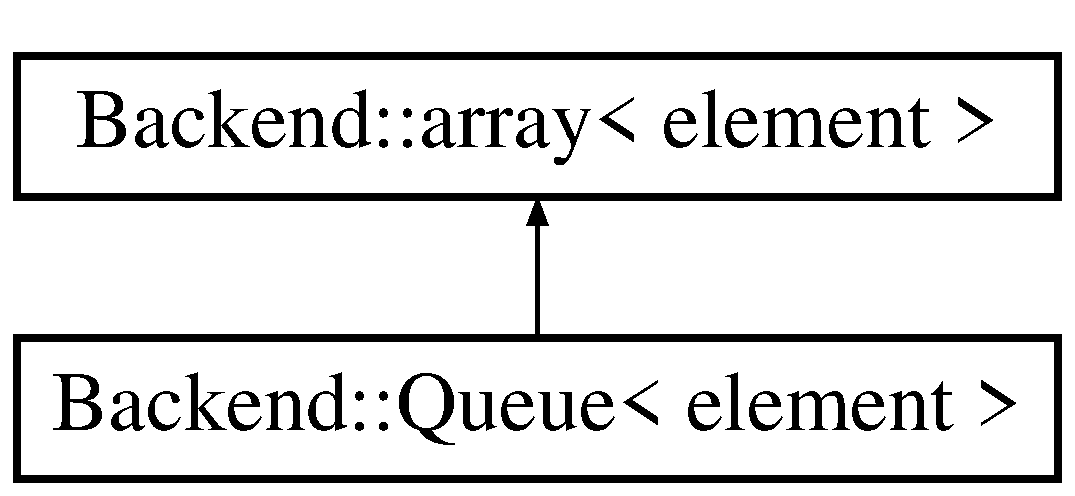
\includegraphics[height=2.000000cm]{classBackend_1_1Queue}
\end{center}
\end{figure}
\subsection*{Public Types}
\begin{DoxyCompactItemize}
\item 
typedef element $\ast$ \hyperlink{classBackend_1_1array_a6d8785dc8b979153ef122f4e3bad1408}{pointer}
\item 
typedef element \& \hyperlink{classBackend_1_1array_aa98075b8d7a4e63ea919ee9d1d4df4a9}{reference}
\end{DoxyCompactItemize}
\subsection*{Public Member Functions}
\begin{DoxyCompactItemize}
\item 
\hyperlink{classBackend_1_1Queue_ac32a0171ecb144e4da8585575160c30c}{Queue} ()
\item 
\hyperlink{classBackend_1_1Queue_ac136488c632785b750fd9fedb5a0986f}{Queue} (unsigned long size)
\item 
\hyperlink{classBackend_1_1Queue_ae7c5f30894c29d332991a15b89aaedba}{Queue} (\hyperlink{classBackend_1_1Queue}{Queue}$<$ element $>$ const \&other)
\item 
\hyperlink{classBackend_1_1Queue}{Queue}$<$ element $>$ \& \hyperlink{classBackend_1_1Queue_a37a138f7a66cbafaab64e10dd9f740e9}{operator=} (\hyperlink{classBackend_1_1Queue}{Queue}$<$ element $>$ const \&other)
\item 
virtual \hyperlink{classBackend_1_1Queue_a9c323720d0c6d433be2a6f5b479e9d47}{$\sim$\+Queue} ()
\item 
bool \hyperlink{classBackend_1_1Queue_aed4ea61ff04a1b2faad6c3f967372bd5}{Write} (element const \&value)
\item 
bool \hyperlink{classBackend_1_1Queue_a10d3583a888cebe4d53863f83249cc13}{Read} (element \&place)
\item 
unsigned long const \& \hyperlink{classBackend_1_1Queue_abb378e040ec42c42b78b10bcb60a933b}{Count} () const 
\item 
bool \hyperlink{classBackend_1_1Queue_acb0a8bd00d4708253e5d25465191dca1}{Full} () const 
\item 
bool \hyperlink{classBackend_1_1Queue_af9f6bfd2928b6a8e0557042da977b9d5}{Empty} () const 
\item 
void \hyperlink{classBackend_1_1Queue_a701ab0dc2289929467d9e1cc5771f80c}{Flush} ()
\item 
element \& \hyperlink{classBackend_1_1array_a906073a0b37d9abef728f2c188e73a5a}{operator\mbox{[}$\,$\mbox{]}} (unsigned long const \&index)
\item 
unsigned long const \& \hyperlink{classBackend_1_1array_a7b74d2da9eacbeea96b1661962a03970}{Size} () const 
\end{DoxyCompactItemize}
\subsection*{Protected Member Functions}
\begin{DoxyCompactItemize}
\item 
unsigned long \hyperlink{classBackend_1_1Queue_a91b2f12926d36b547343a91790fe76bb}{next} (unsigned long value)
\item 
unsigned long \hyperlink{classBackend_1_1Queue_a357667a720d3cf0e1867e79e2911ca13}{make\+\_\+pow\+\_\+2} (unsigned long value)
\end{DoxyCompactItemize}
\subsection*{Protected Attributes}
\begin{DoxyCompactItemize}
\item 
std\+::atomic$<$ unsigned long $>$ \hyperlink{classBackend_1_1Queue_ab3d5c4738092cf356b36c56f6ab61554}{\+\_\+write}
\item 
std\+::atomic$<$ unsigned long $>$ \hyperlink{classBackend_1_1Queue_a508eb8c4fedb73fc4abbf26353bdfd82}{\+\_\+read}
\item 
unsigned long \hyperlink{classBackend_1_1Queue_ab49d17e24dc0f8a2e5e44c182c240249}{\+\_\+count}
\item 
unsigned long \hyperlink{classBackend_1_1Queue_ab665bcab528d6bad6c4faab1ae0fc1b4}{\+\_\+\+M\+A\+S\+K}
\item 
element $\ast$ \hyperlink{classBackend_1_1array_ac588c1e30c2c4748bc9a5bb12b9320af}{\+\_\+array}
\item 
unsigned long \hyperlink{classBackend_1_1array_ae51d64e87b42931946111c28b98e8a18}{\+\_\+size}
\end{DoxyCompactItemize}


\subsection{Detailed Description}
\subsubsection*{template$<$class element$>$class Backend\+::\+Queue$<$ element $>$}



Definition at line 74 of file Queue.\+h.



\subsection{Member Typedef Documentation}
\hypertarget{classBackend_1_1array_a6d8785dc8b979153ef122f4e3bad1408}{\index{Backend\+::\+Queue@{Backend\+::\+Queue}!pointer@{pointer}}
\index{pointer@{pointer}!Backend\+::\+Queue@{Backend\+::\+Queue}}
\subsubsection[{pointer}]{\setlength{\rightskip}{0pt plus 5cm}template$<$class element$>$ typedef element$\ast$ {\bf Backend\+::array}$<$ element $>$\+::{\bf pointer}\hspace{0.3cm}{\ttfamily [inherited]}}}\label{classBackend_1_1array_a6d8785dc8b979153ef122f4e3bad1408}


Definition at line 29 of file Queue.\+h.

\hypertarget{classBackend_1_1array_aa98075b8d7a4e63ea919ee9d1d4df4a9}{\index{Backend\+::\+Queue@{Backend\+::\+Queue}!reference@{reference}}
\index{reference@{reference}!Backend\+::\+Queue@{Backend\+::\+Queue}}
\subsubsection[{reference}]{\setlength{\rightskip}{0pt plus 5cm}template$<$class element$>$ typedef element\& {\bf Backend\+::array}$<$ element $>$\+::{\bf reference}\hspace{0.3cm}{\ttfamily [inherited]}}}\label{classBackend_1_1array_aa98075b8d7a4e63ea919ee9d1d4df4a9}


Definition at line 30 of file Queue.\+h.



\subsection{Constructor \& Destructor Documentation}
\hypertarget{classBackend_1_1Queue_ac32a0171ecb144e4da8585575160c30c}{\index{Backend\+::\+Queue@{Backend\+::\+Queue}!Queue@{Queue}}
\index{Queue@{Queue}!Backend\+::\+Queue@{Backend\+::\+Queue}}
\subsubsection[{Queue}]{\setlength{\rightskip}{0pt plus 5cm}template$<$class element$>$ {\bf Backend\+::\+Queue}$<$ element $>$\+::{\bf Queue} (
\begin{DoxyParamCaption}
{}
\end{DoxyParamCaption}
)\hspace{0.3cm}{\ttfamily [inline]}}}\label{classBackend_1_1Queue_ac32a0171ecb144e4da8585575160c30c}


Definition at line 76 of file Queue.\+h.


\begin{DoxyCode}
76 :array<element>(0),\hyperlink{classBackend_1_1Queue_a508eb8c4fedb73fc4abbf26353bdfd82}{\_read}(0),\hyperlink{classBackend_1_1Queue_ab3d5c4738092cf356b36c56f6ab61554}{\_write}(0),\hyperlink{classBackend_1_1Queue_ab49d17e24dc0f8a2e5e44c182c240249}{\_count}(0),\hyperlink{classBackend_1_1Queue_ab665bcab528d6bad6c4faab1ae0fc1b4}{\_MASK}(0)\{\}
\end{DoxyCode}
\hypertarget{classBackend_1_1Queue_ac136488c632785b750fd9fedb5a0986f}{\index{Backend\+::\+Queue@{Backend\+::\+Queue}!Queue@{Queue}}
\index{Queue@{Queue}!Backend\+::\+Queue@{Backend\+::\+Queue}}
\subsubsection[{Queue}]{\setlength{\rightskip}{0pt plus 5cm}template$<$class element$>$ {\bf Backend\+::\+Queue}$<$ element $>$\+::{\bf Queue} (
\begin{DoxyParamCaption}
\item[{unsigned long}]{size}
\end{DoxyParamCaption}
)\hspace{0.3cm}{\ttfamily [inline]}}}\label{classBackend_1_1Queue_ac136488c632785b750fd9fedb5a0986f}


Definition at line 77 of file Queue.\+h.


\begin{DoxyCode}
77                                  :array<element>(\hyperlink{classBackend_1_1Queue_a357667a720d3cf0e1867e79e2911ca13}{make\_pow\_2}(size)),
      \hyperlink{classBackend_1_1Queue_a508eb8c4fedb73fc4abbf26353bdfd82}{\_read}(0),\hyperlink{classBackend_1_1Queue_ab3d5c4738092cf356b36c56f6ab61554}{\_write}(0),\hyperlink{classBackend_1_1Queue_ab49d17e24dc0f8a2e5e44c182c240249}{\_count}(0)\{
78             \hyperlink{classBackend_1_1Queue_ab665bcab528d6bad6c4faab1ae0fc1b4}{\_MASK} = this->\hyperlink{classBackend_1_1array_ae51d64e87b42931946111c28b98e8a18}{\_size}-1;
79         \}
\end{DoxyCode}
\hypertarget{classBackend_1_1Queue_ae7c5f30894c29d332991a15b89aaedba}{\index{Backend\+::\+Queue@{Backend\+::\+Queue}!Queue@{Queue}}
\index{Queue@{Queue}!Backend\+::\+Queue@{Backend\+::\+Queue}}
\subsubsection[{Queue}]{\setlength{\rightskip}{0pt plus 5cm}template$<$class element$>$ {\bf Backend\+::\+Queue}$<$ element $>$\+::{\bf Queue} (
\begin{DoxyParamCaption}
\item[{{\bf Queue}$<$ element $>$ const \&}]{other}
\end{DoxyParamCaption}
)\hspace{0.3cm}{\ttfamily [inline]}}}\label{classBackend_1_1Queue_ae7c5f30894c29d332991a15b89aaedba}


Definition at line 80 of file Queue.\+h.


\begin{DoxyCode}
80                                           :array<element>(other)\{
81             \hyperlink{classBackend_1_1Queue_ab3d5c4738092cf356b36c56f6ab61554}{\_write}.store(other.\_write.load(std::memory\_order\_acquire));
82             \hyperlink{classBackend_1_1Queue_a508eb8c4fedb73fc4abbf26353bdfd82}{\_read}.store(other.\_read.load(std::memory\_order\_acquire));
83             \hyperlink{classBackend_1_1Queue_ab49d17e24dc0f8a2e5e44c182c240249}{\_count} = other.\_count;
84             \hyperlink{classBackend_1_1Queue_ab665bcab528d6bad6c4faab1ae0fc1b4}{\_MASK} = other.\_size-1;
85         \}
\end{DoxyCode}
\hypertarget{classBackend_1_1Queue_a9c323720d0c6d433be2a6f5b479e9d47}{\index{Backend\+::\+Queue@{Backend\+::\+Queue}!````~Queue@{$\sim$\+Queue}}
\index{````~Queue@{$\sim$\+Queue}!Backend\+::\+Queue@{Backend\+::\+Queue}}
\subsubsection[{$\sim$\+Queue}]{\setlength{\rightskip}{0pt plus 5cm}template$<$class element$>$ virtual {\bf Backend\+::\+Queue}$<$ element $>$\+::$\sim${\bf Queue} (
\begin{DoxyParamCaption}
{}
\end{DoxyParamCaption}
)\hspace{0.3cm}{\ttfamily [inline]}, {\ttfamily [virtual]}}}\label{classBackend_1_1Queue_a9c323720d0c6d433be2a6f5b479e9d47}


Definition at line 94 of file Queue.\+h.


\begin{DoxyCode}
94                         \{
95             \hyperlink{classBackend_1_1Queue_a701ab0dc2289929467d9e1cc5771f80c}{Flush}();
96         \}
\end{DoxyCode}


\subsection{Member Function Documentation}
\hypertarget{classBackend_1_1Queue_abb378e040ec42c42b78b10bcb60a933b}{\index{Backend\+::\+Queue@{Backend\+::\+Queue}!Count@{Count}}
\index{Count@{Count}!Backend\+::\+Queue@{Backend\+::\+Queue}}
\subsubsection[{Count}]{\setlength{\rightskip}{0pt plus 5cm}template$<$class element$>$ unsigned long const\& {\bf Backend\+::\+Queue}$<$ element $>$\+::Count (
\begin{DoxyParamCaption}
{}
\end{DoxyParamCaption}
) const\hspace{0.3cm}{\ttfamily [inline]}}}\label{classBackend_1_1Queue_abb378e040ec42c42b78b10bcb60a933b}


Definition at line 115 of file Queue.\+h.


\begin{DoxyCode}
115                                          \{
116             \textcolor{keywordflow}{return} \hyperlink{classBackend_1_1Queue_ab49d17e24dc0f8a2e5e44c182c240249}{\_count};
117         \}
\end{DoxyCode}
\hypertarget{classBackend_1_1Queue_af9f6bfd2928b6a8e0557042da977b9d5}{\index{Backend\+::\+Queue@{Backend\+::\+Queue}!Empty@{Empty}}
\index{Empty@{Empty}!Backend\+::\+Queue@{Backend\+::\+Queue}}
\subsubsection[{Empty}]{\setlength{\rightskip}{0pt plus 5cm}template$<$class element$>$ bool {\bf Backend\+::\+Queue}$<$ element $>$\+::Empty (
\begin{DoxyParamCaption}
{}
\end{DoxyParamCaption}
) const\hspace{0.3cm}{\ttfamily [inline]}}}\label{classBackend_1_1Queue_af9f6bfd2928b6a8e0557042da977b9d5}


Definition at line 122 of file Queue.\+h.


\begin{DoxyCode}
122                          \{
123             \textcolor{keywordflow}{return} \hyperlink{classBackend_1_1Queue_ab49d17e24dc0f8a2e5e44c182c240249}{\_count}==0;
124         \}
\end{DoxyCode}
\hypertarget{classBackend_1_1Queue_a701ab0dc2289929467d9e1cc5771f80c}{\index{Backend\+::\+Queue@{Backend\+::\+Queue}!Flush@{Flush}}
\index{Flush@{Flush}!Backend\+::\+Queue@{Backend\+::\+Queue}}
\subsubsection[{Flush}]{\setlength{\rightskip}{0pt plus 5cm}template$<$class element$>$ void {\bf Backend\+::\+Queue}$<$ element $>$\+::Flush (
\begin{DoxyParamCaption}
{}
\end{DoxyParamCaption}
)\hspace{0.3cm}{\ttfamily [inline]}}}\label{classBackend_1_1Queue_a701ab0dc2289929467d9e1cc5771f80c}


Definition at line 125 of file Queue.\+h.


\begin{DoxyCode}
125                     \{
126             \hyperlink{classBackend_1_1Queue_ab3d5c4738092cf356b36c56f6ab61554}{\_write}.store(0,std::memory\_order\_relaxed);
127             \hyperlink{classBackend_1_1Queue_a508eb8c4fedb73fc4abbf26353bdfd82}{\_read}.store(0,std::memory\_order\_relaxed);
128             \hyperlink{classBackend_1_1Queue_ab49d17e24dc0f8a2e5e44c182c240249}{\_count}=0;
129         \}
\end{DoxyCode}
\hypertarget{classBackend_1_1Queue_acb0a8bd00d4708253e5d25465191dca1}{\index{Backend\+::\+Queue@{Backend\+::\+Queue}!Full@{Full}}
\index{Full@{Full}!Backend\+::\+Queue@{Backend\+::\+Queue}}
\subsubsection[{Full}]{\setlength{\rightskip}{0pt plus 5cm}template$<$class element$>$ bool {\bf Backend\+::\+Queue}$<$ element $>$\+::Full (
\begin{DoxyParamCaption}
{}
\end{DoxyParamCaption}
) const\hspace{0.3cm}{\ttfamily [inline]}}}\label{classBackend_1_1Queue_acb0a8bd00d4708253e5d25465191dca1}


Definition at line 118 of file Queue.\+h.


\begin{DoxyCode}
118                         \{
119             \textcolor{keywordflow}{return} \hyperlink{classBackend_1_1Queue_ab49d17e24dc0f8a2e5e44c182c240249}{\_count}==this->\hyperlink{classBackend_1_1array_ae51d64e87b42931946111c28b98e8a18}{\_size};
120             
121         \}
\end{DoxyCode}
\hypertarget{classBackend_1_1Queue_a357667a720d3cf0e1867e79e2911ca13}{\index{Backend\+::\+Queue@{Backend\+::\+Queue}!make\+\_\+pow\+\_\+2@{make\+\_\+pow\+\_\+2}}
\index{make\+\_\+pow\+\_\+2@{make\+\_\+pow\+\_\+2}!Backend\+::\+Queue@{Backend\+::\+Queue}}
\subsubsection[{make\+\_\+pow\+\_\+2}]{\setlength{\rightskip}{0pt plus 5cm}template$<$class element$>$ unsigned long {\bf Backend\+::\+Queue}$<$ element $>$\+::make\+\_\+pow\+\_\+2 (
\begin{DoxyParamCaption}
\item[{unsigned long}]{value}
\end{DoxyParamCaption}
)\hspace{0.3cm}{\ttfamily [inline]}, {\ttfamily [protected]}}}\label{classBackend_1_1Queue_a357667a720d3cf0e1867e79e2911ca13}


Definition at line 144 of file Queue.\+h.


\begin{DoxyCode}
144                                                             \{
145             \textcolor{keywordflow}{return} pow(2, ceil(log(value)/log(2)));
146         \}
\end{DoxyCode}
\hypertarget{classBackend_1_1Queue_a91b2f12926d36b547343a91790fe76bb}{\index{Backend\+::\+Queue@{Backend\+::\+Queue}!next@{next}}
\index{next@{next}!Backend\+::\+Queue@{Backend\+::\+Queue}}
\subsubsection[{next}]{\setlength{\rightskip}{0pt plus 5cm}template$<$class element$>$ unsigned long {\bf Backend\+::\+Queue}$<$ element $>$\+::next (
\begin{DoxyParamCaption}
\item[{unsigned long}]{value}
\end{DoxyParamCaption}
)\hspace{0.3cm}{\ttfamily [inline]}, {\ttfamily [protected]}}}\label{classBackend_1_1Queue_a91b2f12926d36b547343a91790fe76bb}


Definition at line 141 of file Queue.\+h.


\begin{DoxyCode}
141                                                       \{
142             \textcolor{keywordflow}{return} (value+1) & \hyperlink{classBackend_1_1Queue_ab665bcab528d6bad6c4faab1ae0fc1b4}{\_MASK};
143         \}
\end{DoxyCode}
\hypertarget{classBackend_1_1Queue_a37a138f7a66cbafaab64e10dd9f740e9}{\index{Backend\+::\+Queue@{Backend\+::\+Queue}!operator=@{operator=}}
\index{operator=@{operator=}!Backend\+::\+Queue@{Backend\+::\+Queue}}
\subsubsection[{operator=}]{\setlength{\rightskip}{0pt plus 5cm}template$<$class element$>$ {\bf Queue}$<$element$>$\& {\bf Backend\+::\+Queue}$<$ element $>$\+::operator= (
\begin{DoxyParamCaption}
\item[{{\bf Queue}$<$ element $>$ const \&}]{other}
\end{DoxyParamCaption}
)\hspace{0.3cm}{\ttfamily [inline]}}}\label{classBackend_1_1Queue_a37a138f7a66cbafaab64e10dd9f740e9}


Definition at line 86 of file Queue.\+h.


\begin{DoxyCode}
86                                                               \{
87             \hyperlink{classBackend_1_1array_abab978602a61af66f73e4951e5779554}{array<element>::operator=}(other);
88             \hyperlink{classBackend_1_1Queue_ab3d5c4738092cf356b36c56f6ab61554}{\_write}.store(other.\_write.load(std::memory\_order\_acquire));
89             \hyperlink{classBackend_1_1Queue_a508eb8c4fedb73fc4abbf26353bdfd82}{\_read}.store(other.\_read.load(std::memory\_order\_acquire));
90             \hyperlink{classBackend_1_1Queue_ab49d17e24dc0f8a2e5e44c182c240249}{\_count} = other.\_count;
91             \hyperlink{classBackend_1_1Queue_ab665bcab528d6bad6c4faab1ae0fc1b4}{\_MASK} = other.\_size-1;
92             \textcolor{keywordflow}{return} *\textcolor{keyword}{this};
93         \}
\end{DoxyCode}
\hypertarget{classBackend_1_1array_a906073a0b37d9abef728f2c188e73a5a}{\index{Backend\+::\+Queue@{Backend\+::\+Queue}!operator\mbox{[}$\,$\mbox{]}@{operator[]}}
\index{operator\mbox{[}$\,$\mbox{]}@{operator[]}!Backend\+::\+Queue@{Backend\+::\+Queue}}
\subsubsection[{operator[]}]{\setlength{\rightskip}{0pt plus 5cm}template$<$class element$>$ element\& {\bf Backend\+::array}$<$ element $>$\+::operator\mbox{[}$\,$\mbox{]} (
\begin{DoxyParamCaption}
\item[{unsigned long const \&}]{index}
\end{DoxyParamCaption}
)\hspace{0.3cm}{\ttfamily [inline]}, {\ttfamily [inherited]}}}\label{classBackend_1_1array_a906073a0b37d9abef728f2c188e73a5a}


Definition at line 58 of file Queue.\+h.


\begin{DoxyCode}
58                                                        \{
59 \textcolor{preprocessor}{#ifdef DEBUG}
60             assert(index<\hyperlink{classBackend_1_1array_ae51d64e87b42931946111c28b98e8a18}{\_size});
61 \textcolor{preprocessor}{#endif}
62             \textcolor{keywordflow}{return} \hyperlink{classBackend_1_1array_ac588c1e30c2c4748bc9a5bb12b9320af}{\_array}[index];
63         \}
\end{DoxyCode}
\hypertarget{classBackend_1_1Queue_a10d3583a888cebe4d53863f83249cc13}{\index{Backend\+::\+Queue@{Backend\+::\+Queue}!Read@{Read}}
\index{Read@{Read}!Backend\+::\+Queue@{Backend\+::\+Queue}}
\subsubsection[{Read}]{\setlength{\rightskip}{0pt plus 5cm}template$<$class element$>$ bool {\bf Backend\+::\+Queue}$<$ element $>$\+::Read (
\begin{DoxyParamCaption}
\item[{element \&}]{place}
\end{DoxyParamCaption}
)\hspace{0.3cm}{\ttfamily [inline]}}}\label{classBackend_1_1Queue_a10d3583a888cebe4d53863f83249cc13}


Definition at line 106 of file Queue.\+h.


\begin{DoxyCode}
106                                  \{
107             \textcolor{keywordflow}{if} (!\hyperlink{classBackend_1_1Queue_af9f6bfd2928b6a8e0557042da977b9d5}{Empty}()) \{
108                 \textcolor{keywordtype}{size\_t} read = \hyperlink{classBackend_1_1Queue_a508eb8c4fedb73fc4abbf26353bdfd82}{\_read}.load(std::memory\_order\_acquire);
109                 \hyperlink{classBackend_1_1Queue_a508eb8c4fedb73fc4abbf26353bdfd82}{\_read}.store(\hyperlink{classBackend_1_1Queue_a91b2f12926d36b547343a91790fe76bb}{next}(read),std::memory\_order\_release);
110                 place = this->\hyperlink{classBackend_1_1array_ac588c1e30c2c4748bc9a5bb12b9320af}{\_array}[read];
111                 --\hyperlink{classBackend_1_1Queue_ab49d17e24dc0f8a2e5e44c182c240249}{\_count};
112                 \textcolor{keywordflow}{return} \textcolor{keyword}{true};
113             \}\textcolor{keywordflow}{else} \textcolor{keywordflow}{return} \textcolor{keyword}{false};
114         \}
\end{DoxyCode}
\hypertarget{classBackend_1_1array_a7b74d2da9eacbeea96b1661962a03970}{\index{Backend\+::\+Queue@{Backend\+::\+Queue}!Size@{Size}}
\index{Size@{Size}!Backend\+::\+Queue@{Backend\+::\+Queue}}
\subsubsection[{Size}]{\setlength{\rightskip}{0pt plus 5cm}template$<$class element$>$ unsigned long const\& {\bf Backend\+::array}$<$ element $>$\+::Size (
\begin{DoxyParamCaption}
{}
\end{DoxyParamCaption}
) const\hspace{0.3cm}{\ttfamily [inline]}, {\ttfamily [inherited]}}}\label{classBackend_1_1array_a7b74d2da9eacbeea96b1661962a03970}


Definition at line 64 of file Queue.\+h.


\begin{DoxyCode}
64                                         \{
65             \textcolor{keywordflow}{return} \hyperlink{classBackend_1_1array_ae51d64e87b42931946111c28b98e8a18}{\_size};
66         \}
\end{DoxyCode}
\hypertarget{classBackend_1_1Queue_aed4ea61ff04a1b2faad6c3f967372bd5}{\index{Backend\+::\+Queue@{Backend\+::\+Queue}!Write@{Write}}
\index{Write@{Write}!Backend\+::\+Queue@{Backend\+::\+Queue}}
\subsubsection[{Write}]{\setlength{\rightskip}{0pt plus 5cm}template$<$class element$>$ bool {\bf Backend\+::\+Queue}$<$ element $>$\+::Write (
\begin{DoxyParamCaption}
\item[{element const \&}]{value}
\end{DoxyParamCaption}
)\hspace{0.3cm}{\ttfamily [inline]}}}\label{classBackend_1_1Queue_aed4ea61ff04a1b2faad6c3f967372bd5}


Definition at line 97 of file Queue.\+h.


\begin{DoxyCode}
97                                         \{
98             \textcolor{keywordflow}{if} (!\hyperlink{classBackend_1_1Queue_acb0a8bd00d4708253e5d25465191dca1}{Full}()) \{
99                 \textcolor{keywordtype}{size\_t} write = \hyperlink{classBackend_1_1Queue_ab3d5c4738092cf356b36c56f6ab61554}{\_write}.load(std::memory\_order\_acquire);
100                 \hyperlink{classBackend_1_1Queue_ab3d5c4738092cf356b36c56f6ab61554}{\_write}.store(\hyperlink{classBackend_1_1Queue_a91b2f12926d36b547343a91790fe76bb}{next}(write),std::memory\_order\_release);
101                 this->\hyperlink{classBackend_1_1array_ac588c1e30c2c4748bc9a5bb12b9320af}{\_array}[write] = value;
102                 ++\hyperlink{classBackend_1_1Queue_ab49d17e24dc0f8a2e5e44c182c240249}{\_count};
103                 \textcolor{keywordflow}{return} \textcolor{keyword}{true};
104             \}\textcolor{keywordflow}{else} \textcolor{keywordflow}{return} \textcolor{keyword}{false};
105         \}
\end{DoxyCode}


\subsection{Member Data Documentation}
\hypertarget{classBackend_1_1array_ac588c1e30c2c4748bc9a5bb12b9320af}{\index{Backend\+::\+Queue@{Backend\+::\+Queue}!\+\_\+array@{\+\_\+array}}
\index{\+\_\+array@{\+\_\+array}!Backend\+::\+Queue@{Backend\+::\+Queue}}
\subsubsection[{\+\_\+array}]{\setlength{\rightskip}{0pt plus 5cm}template$<$class element$>$ element$\ast$ {\bf Backend\+::array}$<$ element $>$\+::\+\_\+array\hspace{0.3cm}{\ttfamily [protected]}, {\ttfamily [inherited]}}}\label{classBackend_1_1array_ac588c1e30c2c4748bc9a5bb12b9320af}


Definition at line 68 of file Queue.\+h.

\hypertarget{classBackend_1_1Queue_ab49d17e24dc0f8a2e5e44c182c240249}{\index{Backend\+::\+Queue@{Backend\+::\+Queue}!\+\_\+count@{\+\_\+count}}
\index{\+\_\+count@{\+\_\+count}!Backend\+::\+Queue@{Backend\+::\+Queue}}
\subsubsection[{\+\_\+count}]{\setlength{\rightskip}{0pt plus 5cm}template$<$class element$>$ unsigned long {\bf Backend\+::\+Queue}$<$ element $>$\+::\+\_\+count\hspace{0.3cm}{\ttfamily [protected]}}}\label{classBackend_1_1Queue_ab49d17e24dc0f8a2e5e44c182c240249}


Definition at line 139 of file Queue.\+h.

\hypertarget{classBackend_1_1Queue_ab665bcab528d6bad6c4faab1ae0fc1b4}{\index{Backend\+::\+Queue@{Backend\+::\+Queue}!\+\_\+\+M\+A\+S\+K@{\+\_\+\+M\+A\+S\+K}}
\index{\+\_\+\+M\+A\+S\+K@{\+\_\+\+M\+A\+S\+K}!Backend\+::\+Queue@{Backend\+::\+Queue}}
\subsubsection[{\+\_\+\+M\+A\+S\+K}]{\setlength{\rightskip}{0pt plus 5cm}template$<$class element$>$ unsigned long {\bf Backend\+::\+Queue}$<$ element $>$\+::\+\_\+\+M\+A\+S\+K\hspace{0.3cm}{\ttfamily [protected]}}}\label{classBackend_1_1Queue_ab665bcab528d6bad6c4faab1ae0fc1b4}


Definition at line 140 of file Queue.\+h.

\hypertarget{classBackend_1_1Queue_a508eb8c4fedb73fc4abbf26353bdfd82}{\index{Backend\+::\+Queue@{Backend\+::\+Queue}!\+\_\+read@{\+\_\+read}}
\index{\+\_\+read@{\+\_\+read}!Backend\+::\+Queue@{Backend\+::\+Queue}}
\subsubsection[{\+\_\+read}]{\setlength{\rightskip}{0pt plus 5cm}template$<$class element$>$ std\+::atomic$<$unsigned long$>$ {\bf Backend\+::\+Queue}$<$ element $>$\+::\+\_\+read\hspace{0.3cm}{\ttfamily [protected]}}}\label{classBackend_1_1Queue_a508eb8c4fedb73fc4abbf26353bdfd82}


Definition at line 138 of file Queue.\+h.

\hypertarget{classBackend_1_1array_ae51d64e87b42931946111c28b98e8a18}{\index{Backend\+::\+Queue@{Backend\+::\+Queue}!\+\_\+size@{\+\_\+size}}
\index{\+\_\+size@{\+\_\+size}!Backend\+::\+Queue@{Backend\+::\+Queue}}
\subsubsection[{\+\_\+size}]{\setlength{\rightskip}{0pt plus 5cm}template$<$class element$>$ unsigned long {\bf Backend\+::array}$<$ element $>$\+::\+\_\+size\hspace{0.3cm}{\ttfamily [protected]}, {\ttfamily [inherited]}}}\label{classBackend_1_1array_ae51d64e87b42931946111c28b98e8a18}


Definition at line 69 of file Queue.\+h.

\hypertarget{classBackend_1_1Queue_ab3d5c4738092cf356b36c56f6ab61554}{\index{Backend\+::\+Queue@{Backend\+::\+Queue}!\+\_\+write@{\+\_\+write}}
\index{\+\_\+write@{\+\_\+write}!Backend\+::\+Queue@{Backend\+::\+Queue}}
\subsubsection[{\+\_\+write}]{\setlength{\rightskip}{0pt plus 5cm}template$<$class element$>$ std\+::atomic$<$unsigned long$>$ {\bf Backend\+::\+Queue}$<$ element $>$\+::\+\_\+write\hspace{0.3cm}{\ttfamily [protected]}}}\label{classBackend_1_1Queue_ab3d5c4738092cf356b36c56f6ab61554}


Definition at line 137 of file Queue.\+h.



The documentation for this class was generated from the following file\+:\begin{DoxyCompactItemize}
\item 
/\+Users/alexanderzywicki/\+Documents/\+School\+\_\+\+Stuff/\+Fall\+\_\+2014/\+Digital\+\_\+\+Signal\+\_\+\+Generation\+\_\+and\+\_\+\+Analysis/src/include/\hyperlink{Queue_8h}{Queue.\+h}\end{DoxyCompactItemize}

\hypertarget{classSignal_1_1RingBuffer}{\section{Signal\+:\+:Ring\+Buffer Class Reference}
\label{classSignal_1_1RingBuffer}\index{Signal\+::\+Ring\+Buffer@{Signal\+::\+Ring\+Buffer}}
}


{\ttfamily \#include $<$Ring\+Buffer.\+h$>$}

Inheritance diagram for Signal\+:\+:Ring\+Buffer\+:\begin{figure}[H]
\begin{center}
\leavevmode
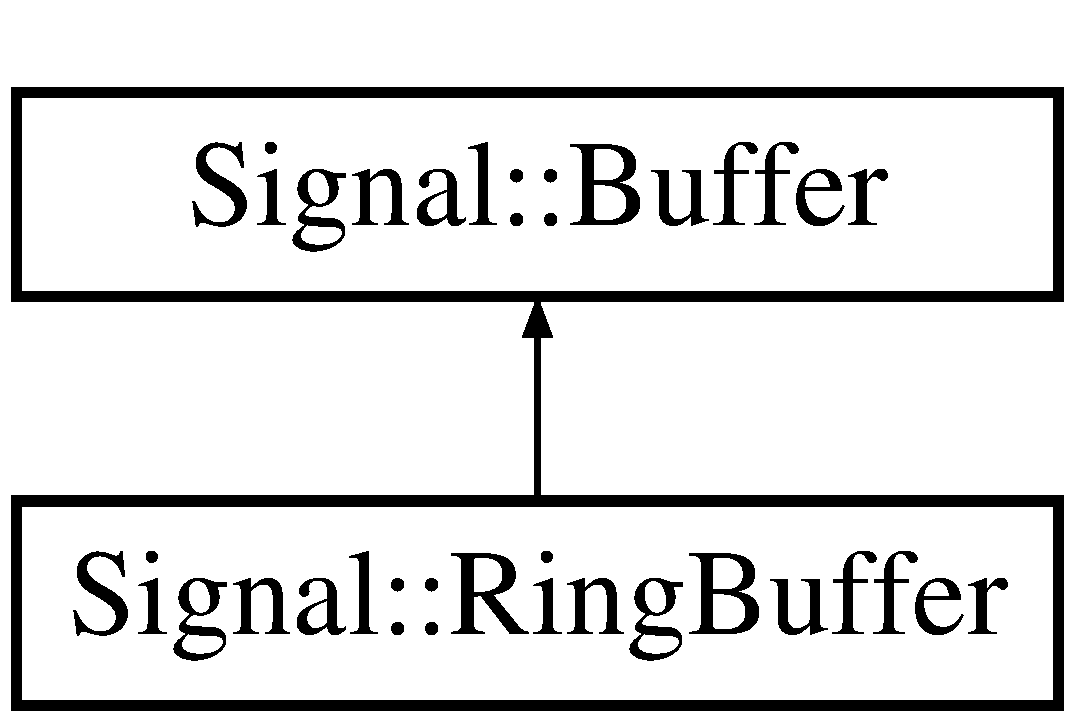
\includegraphics[height=2.000000cm]{classSignal_1_1RingBuffer}
\end{center}
\end{figure}
\subsection*{Public Member Functions}
\begin{DoxyCompactItemize}
\item 
\hyperlink{classSignal_1_1RingBuffer_a66b2a49fc1ea8d4e2d529362452a9e5e}{Ring\+Buffer} ()
\item 
\hyperlink{classSignal_1_1RingBuffer_aab0efff6a85c76ce9063b6a7dcc1fe97}{Ring\+Buffer} (const size\+\_\+t size)
\item 
\hyperlink{classSignal_1_1RingBuffer_a9823e69bede828ca41cdf0b8372224f7}{Ring\+Buffer} (\hyperlink{classSignal_1_1RingBuffer}{Ring\+Buffer} \&buffer)
\item 
\hyperlink{classSignal_1_1RingBuffer}{Ring\+Buffer} \& \hyperlink{classSignal_1_1RingBuffer_a2bc19d3eb407be62e36ac327bffe4b2f}{operator=} (\hyperlink{classSignal_1_1RingBuffer}{Ring\+Buffer} \&buffer)
\item 
virtual \hyperlink{classSignal_1_1RingBuffer_aff2a78175f358585ddf207f470062d3e}{$\sim$\+Ring\+Buffer} ()
\item 
bool \hyperlink{classSignal_1_1RingBuffer_aa291195b777aa50aa7a61ab1f4954bce}{Write} (const \hyperlink{classSignal_1_1Sample}{Signal\+::\+Sample} \&elem)
\item 
bool \hyperlink{classSignal_1_1RingBuffer_a9a5c8429c0e422e3d4763adb78b0a87c}{Read} (\hyperlink{classSignal_1_1Sample}{Signal\+::\+Sample} \&elem)
\item 
size\+\_\+t const \& \hyperlink{classSignal_1_1RingBuffer_acf6e81f09bb9f10a79ced6da84e78e20}{Count} () const 
\item 
bool \hyperlink{classSignal_1_1RingBuffer_ac8124016cfc0c833a3565c87d5f6f1e5}{Full} () const 
\item 
bool \hyperlink{classSignal_1_1RingBuffer_a73416d725604567d4b496f9821bc0c04}{Empty} () const 
\item 
void \hyperlink{classSignal_1_1RingBuffer_aa9d2938e5c11c5d3c058db9b7e310406}{Flush} ()
\item 
\hyperlink{classSignal_1_1Sample}{Signal\+::\+Sample} \& \hyperlink{classSignal_1_1Buffer_a0b4ced776c42720b214f6054fa21547a}{operator\mbox{[}$\,$\mbox{]}} (size\+\_\+t const \&index)
\item 
size\+\_\+t const \& \hyperlink{classSignal_1_1Buffer_ad0350078d641ed5cb15a9401d9d20ffe}{Size} () const 
\end{DoxyCompactItemize}
\subsection*{Protected Member Functions}
\begin{DoxyCompactItemize}
\item 
size\+\_\+t \hyperlink{classSignal_1_1RingBuffer_a14a5990d51a45d131ee8aebd90bb87b9}{next} (size\+\_\+t current)
\item 
size\+\_\+t \hyperlink{classSignal_1_1RingBuffer_ae81c9b6959e18edabd54a073b936db0c}{make\+\_\+pow\+\_\+2} (size\+\_\+t number)
\end{DoxyCompactItemize}
\subsection*{Protected Attributes}
\begin{DoxyCompactItemize}
\item 
std\+::atomic$<$ size\+\_\+t $>$ \hyperlink{classSignal_1_1RingBuffer_a121cbb3679c61132fad237c671d08bef}{\+\_\+write}
\item 
std\+::atomic$<$ size\+\_\+t $>$ \hyperlink{classSignal_1_1RingBuffer_a4bdf5d626567f423b480398aef2e8bb0}{\+\_\+read}
\item 
size\+\_\+t \hyperlink{classSignal_1_1RingBuffer_ab41dbb1bd8c572099349f92055ed9185}{\+\_\+count}
\item 
size\+\_\+t \hyperlink{classSignal_1_1RingBuffer_a6f0dc159e6d625b8352988c6a0577ffe}{M\+A\+S\+K}
\item 
\hyperlink{classSignal_1_1Sample}{Signal\+::\+Sample} $\ast$ \hyperlink{classSignal_1_1Buffer_ae88831d6fdf8fd7591d5dd7f79531d5f}{\+\_\+buffer}
\item 
size\+\_\+t \hyperlink{classSignal_1_1Buffer_ab4c8969e972323306ee51538ad70577b}{\+\_\+size}
\end{DoxyCompactItemize}


\subsection{Detailed Description}


Definition at line 24 of file Ring\+Buffer.\+h.



\subsection{Constructor \& Destructor Documentation}
\hypertarget{classSignal_1_1RingBuffer_a66b2a49fc1ea8d4e2d529362452a9e5e}{\index{Signal\+::\+Ring\+Buffer@{Signal\+::\+Ring\+Buffer}!Ring\+Buffer@{Ring\+Buffer}}
\index{Ring\+Buffer@{Ring\+Buffer}!Signal\+::\+Ring\+Buffer@{Signal\+::\+Ring\+Buffer}}
\subsubsection[{Ring\+Buffer}]{\setlength{\rightskip}{0pt plus 5cm}Signal\+::\+Ring\+Buffer\+::\+Ring\+Buffer (
\begin{DoxyParamCaption}
{}
\end{DoxyParamCaption}
)}}\label{classSignal_1_1RingBuffer_a66b2a49fc1ea8d4e2d529362452a9e5e}


Definition at line 14 of file Ring\+Buffer.\+cpp.


\begin{DoxyCode}
14 :\hyperlink{classSignal_1_1Buffer_ab558e80dac4ef396b9c9310fd914936f}{Buffer}(0),\hyperlink{classSignal_1_1RingBuffer_a4bdf5d626567f423b480398aef2e8bb0}{\_read}(0),\hyperlink{classSignal_1_1RingBuffer_a121cbb3679c61132fad237c671d08bef}{\_write}(0),\hyperlink{classSignal_1_1RingBuffer_ab41dbb1bd8c572099349f92055ed9185}{\_count}(0),\hyperlink{classSignal_1_1RingBuffer_a6f0dc159e6d625b8352988c6a0577ffe}{MASK}(0)\{\}
\end{DoxyCode}
\hypertarget{classSignal_1_1RingBuffer_aab0efff6a85c76ce9063b6a7dcc1fe97}{\index{Signal\+::\+Ring\+Buffer@{Signal\+::\+Ring\+Buffer}!Ring\+Buffer@{Ring\+Buffer}}
\index{Ring\+Buffer@{Ring\+Buffer}!Signal\+::\+Ring\+Buffer@{Signal\+::\+Ring\+Buffer}}
\subsubsection[{Ring\+Buffer}]{\setlength{\rightskip}{0pt plus 5cm}Signal\+::\+Ring\+Buffer\+::\+Ring\+Buffer (
\begin{DoxyParamCaption}
\item[{const size\+\_\+t}]{size}
\end{DoxyParamCaption}
)}}\label{classSignal_1_1RingBuffer_aab0efff6a85c76ce9063b6a7dcc1fe97}


Definition at line 16 of file Ring\+Buffer.\+cpp.


\begin{DoxyCode}
16                                              :\hyperlink{classSignal_1_1Buffer_ab558e80dac4ef396b9c9310fd914936f}{Buffer}(\hyperlink{classSignal_1_1RingBuffer_ae81c9b6959e18edabd54a073b936db0c}{make\_pow\_2}(size)),
      \hyperlink{classSignal_1_1RingBuffer_a4bdf5d626567f423b480398aef2e8bb0}{\_read}(0),\hyperlink{classSignal_1_1RingBuffer_a121cbb3679c61132fad237c671d08bef}{\_write}(0),\hyperlink{classSignal_1_1RingBuffer_ab41dbb1bd8c572099349f92055ed9185}{\_count}(0)\{
17     \hyperlink{classSignal_1_1RingBuffer_a6f0dc159e6d625b8352988c6a0577ffe}{MASK} = this->\hyperlink{classSignal_1_1Buffer_ab4c8969e972323306ee51538ad70577b}{\_size}-1;
18 \}
\end{DoxyCode}
\hypertarget{classSignal_1_1RingBuffer_a9823e69bede828ca41cdf0b8372224f7}{\index{Signal\+::\+Ring\+Buffer@{Signal\+::\+Ring\+Buffer}!Ring\+Buffer@{Ring\+Buffer}}
\index{Ring\+Buffer@{Ring\+Buffer}!Signal\+::\+Ring\+Buffer@{Signal\+::\+Ring\+Buffer}}
\subsubsection[{Ring\+Buffer}]{\setlength{\rightskip}{0pt plus 5cm}Signal\+::\+Ring\+Buffer\+::\+Ring\+Buffer (
\begin{DoxyParamCaption}
\item[{{\bf Ring\+Buffer} \&}]{buffer}
\end{DoxyParamCaption}
)}}\label{classSignal_1_1RingBuffer_a9823e69bede828ca41cdf0b8372224f7}


Definition at line 20 of file Ring\+Buffer.\+cpp.


\begin{DoxyCode}
20                                               :\hyperlink{classSignal_1_1Buffer_ab558e80dac4ef396b9c9310fd914936f}{Buffer}(buffer)\{
21     \hyperlink{classSignal_1_1RingBuffer_a121cbb3679c61132fad237c671d08bef}{\_write}.store(buffer.\_write.load(std::memory\_order\_acquire));
22     \hyperlink{classSignal_1_1RingBuffer_a4bdf5d626567f423b480398aef2e8bb0}{\_read}.store(buffer.\_read.load(std::memory\_order\_acquire));
23     \hyperlink{classSignal_1_1RingBuffer_ab41dbb1bd8c572099349f92055ed9185}{\_count} = buffer.\_count;
24     \hyperlink{classSignal_1_1RingBuffer_a6f0dc159e6d625b8352988c6a0577ffe}{MASK} = buffer.\_size-1;
25 \}
\end{DoxyCode}
\hypertarget{classSignal_1_1RingBuffer_aff2a78175f358585ddf207f470062d3e}{\index{Signal\+::\+Ring\+Buffer@{Signal\+::\+Ring\+Buffer}!````~Ring\+Buffer@{$\sim$\+Ring\+Buffer}}
\index{````~Ring\+Buffer@{$\sim$\+Ring\+Buffer}!Signal\+::\+Ring\+Buffer@{Signal\+::\+Ring\+Buffer}}
\subsubsection[{$\sim$\+Ring\+Buffer}]{\setlength{\rightskip}{0pt plus 5cm}Signal\+::\+Ring\+Buffer\+::$\sim$\+Ring\+Buffer (
\begin{DoxyParamCaption}
{}
\end{DoxyParamCaption}
)\hspace{0.3cm}{\ttfamily [virtual]}}}\label{classSignal_1_1RingBuffer_aff2a78175f358585ddf207f470062d3e}


Definition at line 35 of file Ring\+Buffer.\+cpp.


\begin{DoxyCode}
35 \{\hyperlink{classSignal_1_1RingBuffer_aa9d2938e5c11c5d3c058db9b7e310406}{Flush}();\}
\end{DoxyCode}


\subsection{Member Function Documentation}
\hypertarget{classSignal_1_1RingBuffer_acf6e81f09bb9f10a79ced6da84e78e20}{\index{Signal\+::\+Ring\+Buffer@{Signal\+::\+Ring\+Buffer}!Count@{Count}}
\index{Count@{Count}!Signal\+::\+Ring\+Buffer@{Signal\+::\+Ring\+Buffer}}
\subsubsection[{Count}]{\setlength{\rightskip}{0pt plus 5cm}size\+\_\+t const \& Signal\+::\+Ring\+Buffer\+::\+Count (
\begin{DoxyParamCaption}
{}
\end{DoxyParamCaption}
) const\hspace{0.3cm}{\ttfamily [inline]}}}\label{classSignal_1_1RingBuffer_acf6e81f09bb9f10a79ced6da84e78e20}


Definition at line 77 of file Ring\+Buffer.\+h.


\begin{DoxyCode}
77                                                \{
78         \textcolor{keywordflow}{return} \hyperlink{classSignal_1_1RingBuffer_ab41dbb1bd8c572099349f92055ed9185}{\_count};
79     \}
\end{DoxyCode}
\hypertarget{classSignal_1_1RingBuffer_a73416d725604567d4b496f9821bc0c04}{\index{Signal\+::\+Ring\+Buffer@{Signal\+::\+Ring\+Buffer}!Empty@{Empty}}
\index{Empty@{Empty}!Signal\+::\+Ring\+Buffer@{Signal\+::\+Ring\+Buffer}}
\subsubsection[{Empty}]{\setlength{\rightskip}{0pt plus 5cm}bool Signal\+::\+Ring\+Buffer\+::\+Empty (
\begin{DoxyParamCaption}
{}
\end{DoxyParamCaption}
) const\hspace{0.3cm}{\ttfamily [inline]}}}\label{classSignal_1_1RingBuffer_a73416d725604567d4b496f9821bc0c04}


Definition at line 51 of file Ring\+Buffer.\+h.


\begin{DoxyCode}
51                                       \{
52         \textcolor{keywordflow}{return} \hyperlink{classSignal_1_1RingBuffer_ab41dbb1bd8c572099349f92055ed9185}{\_count}==0;
53     \}
\end{DoxyCode}
\hypertarget{classSignal_1_1RingBuffer_aa9d2938e5c11c5d3c058db9b7e310406}{\index{Signal\+::\+Ring\+Buffer@{Signal\+::\+Ring\+Buffer}!Flush@{Flush}}
\index{Flush@{Flush}!Signal\+::\+Ring\+Buffer@{Signal\+::\+Ring\+Buffer}}
\subsubsection[{Flush}]{\setlength{\rightskip}{0pt plus 5cm}void Signal\+::\+Ring\+Buffer\+::\+Flush (
\begin{DoxyParamCaption}
{}
\end{DoxyParamCaption}
)\hspace{0.3cm}{\ttfamily [inline]}}}\label{classSignal_1_1RingBuffer_aa9d2938e5c11c5d3c058db9b7e310406}


Definition at line 54 of file Ring\+Buffer.\+h.


\begin{DoxyCode}
54                                  \{
55         \hyperlink{classSignal_1_1RingBuffer_a121cbb3679c61132fad237c671d08bef}{\_write}.store(0,std::memory\_order\_relaxed);
56         \hyperlink{classSignal_1_1RingBuffer_a4bdf5d626567f423b480398aef2e8bb0}{\_read}.store(0,std::memory\_order\_relaxed);
57         \hyperlink{classSignal_1_1RingBuffer_ab41dbb1bd8c572099349f92055ed9185}{\_count}=0;
58     \}
\end{DoxyCode}
\hypertarget{classSignal_1_1RingBuffer_ac8124016cfc0c833a3565c87d5f6f1e5}{\index{Signal\+::\+Ring\+Buffer@{Signal\+::\+Ring\+Buffer}!Full@{Full}}
\index{Full@{Full}!Signal\+::\+Ring\+Buffer@{Signal\+::\+Ring\+Buffer}}
\subsubsection[{Full}]{\setlength{\rightskip}{0pt plus 5cm}bool Signal\+::\+Ring\+Buffer\+::\+Full (
\begin{DoxyParamCaption}
{}
\end{DoxyParamCaption}
) const\hspace{0.3cm}{\ttfamily [inline]}}}\label{classSignal_1_1RingBuffer_ac8124016cfc0c833a3565c87d5f6f1e5}


Definition at line 48 of file Ring\+Buffer.\+h.


\begin{DoxyCode}
48                                      \{
49         \textcolor{keywordflow}{return} \hyperlink{classSignal_1_1RingBuffer_ab41dbb1bd8c572099349f92055ed9185}{\_count}==this->\hyperlink{classSignal_1_1Buffer_ab4c8969e972323306ee51538ad70577b}{\_size};
50     \}
\end{DoxyCode}
\hypertarget{classSignal_1_1RingBuffer_ae81c9b6959e18edabd54a073b936db0c}{\index{Signal\+::\+Ring\+Buffer@{Signal\+::\+Ring\+Buffer}!make\+\_\+pow\+\_\+2@{make\+\_\+pow\+\_\+2}}
\index{make\+\_\+pow\+\_\+2@{make\+\_\+pow\+\_\+2}!Signal\+::\+Ring\+Buffer@{Signal\+::\+Ring\+Buffer}}
\subsubsection[{make\+\_\+pow\+\_\+2}]{\setlength{\rightskip}{0pt plus 5cm}size\+\_\+t Signal\+::\+Ring\+Buffer\+::make\+\_\+pow\+\_\+2 (
\begin{DoxyParamCaption}
\item[{size\+\_\+t}]{number}
\end{DoxyParamCaption}
)\hspace{0.3cm}{\ttfamily [inline]}, {\ttfamily [protected]}}}\label{classSignal_1_1RingBuffer_ae81c9b6959e18edabd54a073b936db0c}


Definition at line 83 of file Ring\+Buffer.\+h.


\begin{DoxyCode}
83                                                      \{
84         \textcolor{keywordflow}{return} pow(2, ceil(log(number)/log(2)));
85     \}
\end{DoxyCode}
\hypertarget{classSignal_1_1RingBuffer_a14a5990d51a45d131ee8aebd90bb87b9}{\index{Signal\+::\+Ring\+Buffer@{Signal\+::\+Ring\+Buffer}!next@{next}}
\index{next@{next}!Signal\+::\+Ring\+Buffer@{Signal\+::\+Ring\+Buffer}}
\subsubsection[{next}]{\setlength{\rightskip}{0pt plus 5cm}size\+\_\+t Signal\+::\+Ring\+Buffer\+::next (
\begin{DoxyParamCaption}
\item[{size\+\_\+t}]{current}
\end{DoxyParamCaption}
)\hspace{0.3cm}{\ttfamily [inline]}, {\ttfamily [protected]}}}\label{classSignal_1_1RingBuffer_a14a5990d51a45d131ee8aebd90bb87b9}


Definition at line 82 of file Ring\+Buffer.\+h.


\begin{DoxyCode}
82 \{\textcolor{keywordflow}{return} (current+1) & \hyperlink{classSignal_1_1RingBuffer_a6f0dc159e6d625b8352988c6a0577ffe}{MASK};\}
\end{DoxyCode}
\hypertarget{classSignal_1_1RingBuffer_a2bc19d3eb407be62e36ac327bffe4b2f}{\index{Signal\+::\+Ring\+Buffer@{Signal\+::\+Ring\+Buffer}!operator=@{operator=}}
\index{operator=@{operator=}!Signal\+::\+Ring\+Buffer@{Signal\+::\+Ring\+Buffer}}
\subsubsection[{operator=}]{\setlength{\rightskip}{0pt plus 5cm}{\bf Signal\+::\+Ring\+Buffer} \& Signal\+::\+Ring\+Buffer\+::operator= (
\begin{DoxyParamCaption}
\item[{{\bf Ring\+Buffer} \&}]{buffer}
\end{DoxyParamCaption}
)}}\label{classSignal_1_1RingBuffer_a2bc19d3eb407be62e36ac327bffe4b2f}


Definition at line 27 of file Ring\+Buffer.\+cpp.


\begin{DoxyCode}
27                                                                \{
28     \hyperlink{classSignal_1_1Buffer_a9f9f08e2cdf35d15164997455303a2d9}{Buffer::operator=}(buffer);
29     \hyperlink{classSignal_1_1RingBuffer_a121cbb3679c61132fad237c671d08bef}{\_write}.store(buffer.\_write.load(std::memory\_order\_acquire));
30     \hyperlink{classSignal_1_1RingBuffer_a4bdf5d626567f423b480398aef2e8bb0}{\_read}.store(buffer.\_read.load(std::memory\_order\_acquire));
31     \hyperlink{classSignal_1_1RingBuffer_ab41dbb1bd8c572099349f92055ed9185}{\_count} = buffer.\_count;
32     \hyperlink{classSignal_1_1RingBuffer_a6f0dc159e6d625b8352988c6a0577ffe}{MASK} = buffer.\_size-1;
33     \textcolor{keywordflow}{return} *\textcolor{keyword}{this};
34 \}
\end{DoxyCode}
\hypertarget{classSignal_1_1Buffer_a0b4ced776c42720b214f6054fa21547a}{\index{Signal\+::\+Ring\+Buffer@{Signal\+::\+Ring\+Buffer}!operator\mbox{[}$\,$\mbox{]}@{operator[]}}
\index{operator\mbox{[}$\,$\mbox{]}@{operator[]}!Signal\+::\+Ring\+Buffer@{Signal\+::\+Ring\+Buffer}}
\subsubsection[{operator[]}]{\setlength{\rightskip}{0pt plus 5cm}{\bf Signal\+::\+Sample} \& Signal\+::\+Buffer\+::operator\mbox{[}$\,$\mbox{]} (
\begin{DoxyParamCaption}
\item[{size\+\_\+t const \&}]{index}
\end{DoxyParamCaption}
)\hspace{0.3cm}{\ttfamily [inherited]}}}\label{classSignal_1_1Buffer_a0b4ced776c42720b214f6054fa21547a}


Definition at line 38 of file Buffer.\+cpp.


\begin{DoxyCode}
38                                                          \{
39 \textcolor{preprocessor}{#ifdef DEBUG}
40     assert(index<\hyperlink{classSignal_1_1Buffer_ab4c8969e972323306ee51538ad70577b}{\_size});
41 \textcolor{preprocessor}{#endif}
42     \textcolor{keywordflow}{return} \hyperlink{classSignal_1_1Buffer_ae88831d6fdf8fd7591d5dd7f79531d5f}{\_buffer}[index];
43 \}
\end{DoxyCode}
\hypertarget{classSignal_1_1RingBuffer_a9a5c8429c0e422e3d4763adb78b0a87c}{\index{Signal\+::\+Ring\+Buffer@{Signal\+::\+Ring\+Buffer}!Read@{Read}}
\index{Read@{Read}!Signal\+::\+Ring\+Buffer@{Signal\+::\+Ring\+Buffer}}
\subsubsection[{Read}]{\setlength{\rightskip}{0pt plus 5cm}bool Signal\+::\+Ring\+Buffer\+::\+Read (
\begin{DoxyParamCaption}
\item[{{\bf Signal\+::\+Sample} \&}]{elem}
\end{DoxyParamCaption}
)\hspace{0.3cm}{\ttfamily [inline]}}}\label{classSignal_1_1RingBuffer_a9a5c8429c0e422e3d4763adb78b0a87c}


Definition at line 68 of file Ring\+Buffer.\+h.


\begin{DoxyCode}
68                                                   \{
69         \textcolor{keywordflow}{if} (!\hyperlink{classSignal_1_1RingBuffer_a73416d725604567d4b496f9821bc0c04}{Empty}()) \{
70             \textcolor{keywordtype}{size\_t} read = \hyperlink{classSignal_1_1RingBuffer_a4bdf5d626567f423b480398aef2e8bb0}{\_read}.load(std::memory\_order\_acquire);
71             \hyperlink{classSignal_1_1RingBuffer_a4bdf5d626567f423b480398aef2e8bb0}{\_read}.store(\hyperlink{classSignal_1_1RingBuffer_a14a5990d51a45d131ee8aebd90bb87b9}{next}(read),std::memory\_order\_release);
72             elem = this->\hyperlink{classSignal_1_1Buffer_ae88831d6fdf8fd7591d5dd7f79531d5f}{\_buffer}[read];
73             --\hyperlink{classSignal_1_1RingBuffer_ab41dbb1bd8c572099349f92055ed9185}{\_count};
74             \textcolor{keywordflow}{return} \textcolor{keyword}{true};
75         \}\textcolor{keywordflow}{else} \textcolor{keywordflow}{return} \textcolor{keyword}{false};
76     \}
\end{DoxyCode}
\hypertarget{classSignal_1_1Buffer_ad0350078d641ed5cb15a9401d9d20ffe}{\index{Signal\+::\+Ring\+Buffer@{Signal\+::\+Ring\+Buffer}!Size@{Size}}
\index{Size@{Size}!Signal\+::\+Ring\+Buffer@{Signal\+::\+Ring\+Buffer}}
\subsubsection[{Size}]{\setlength{\rightskip}{0pt plus 5cm}size\+\_\+t const \& Signal\+::\+Buffer\+::\+Size (
\begin{DoxyParamCaption}
{}
\end{DoxyParamCaption}
) const\hspace{0.3cm}{\ttfamily [inline]}, {\ttfamily [inherited]}}}\label{classSignal_1_1Buffer_ad0350078d641ed5cb15a9401d9d20ffe}


Definition at line 31 of file Buffer.\+h.


\begin{DoxyCode}
31                                           \{
32         \textcolor{keywordflow}{return} \hyperlink{classSignal_1_1Buffer_ab4c8969e972323306ee51538ad70577b}{\_size};
33     \}
\end{DoxyCode}
\hypertarget{classSignal_1_1RingBuffer_aa291195b777aa50aa7a61ab1f4954bce}{\index{Signal\+::\+Ring\+Buffer@{Signal\+::\+Ring\+Buffer}!Write@{Write}}
\index{Write@{Write}!Signal\+::\+Ring\+Buffer@{Signal\+::\+Ring\+Buffer}}
\subsubsection[{Write}]{\setlength{\rightskip}{0pt plus 5cm}bool Signal\+::\+Ring\+Buffer\+::\+Write (
\begin{DoxyParamCaption}
\item[{const {\bf Signal\+::\+Sample} \&}]{elem}
\end{DoxyParamCaption}
)\hspace{0.3cm}{\ttfamily [inline]}}}\label{classSignal_1_1RingBuffer_aa291195b777aa50aa7a61ab1f4954bce}


Definition at line 59 of file Ring\+Buffer.\+h.


\begin{DoxyCode}
59                                                          \{
60         \textcolor{keywordflow}{if} (!\hyperlink{classSignal_1_1RingBuffer_ac8124016cfc0c833a3565c87d5f6f1e5}{Full}()) \{
61             \textcolor{keywordtype}{size\_t} write = \hyperlink{classSignal_1_1RingBuffer_a121cbb3679c61132fad237c671d08bef}{\_write}.load(std::memory\_order\_acquire);
62             \hyperlink{classSignal_1_1RingBuffer_a121cbb3679c61132fad237c671d08bef}{\_write}.store(\hyperlink{classSignal_1_1RingBuffer_a14a5990d51a45d131ee8aebd90bb87b9}{next}(write),std::memory\_order\_release);
63             this->\hyperlink{classSignal_1_1Buffer_ae88831d6fdf8fd7591d5dd7f79531d5f}{\_buffer}[write] = elem;
64             ++\hyperlink{classSignal_1_1RingBuffer_ab41dbb1bd8c572099349f92055ed9185}{\_count};
65             \textcolor{keywordflow}{return} \textcolor{keyword}{true};
66         \}\textcolor{keywordflow}{else} \textcolor{keywordflow}{return} \textcolor{keyword}{false};
67     \}
\end{DoxyCode}


\subsection{Member Data Documentation}
\hypertarget{classSignal_1_1Buffer_ae88831d6fdf8fd7591d5dd7f79531d5f}{\index{Signal\+::\+Ring\+Buffer@{Signal\+::\+Ring\+Buffer}!\+\_\+buffer@{\+\_\+buffer}}
\index{\+\_\+buffer@{\+\_\+buffer}!Signal\+::\+Ring\+Buffer@{Signal\+::\+Ring\+Buffer}}
\subsubsection[{\+\_\+buffer}]{\setlength{\rightskip}{0pt plus 5cm}{\bf Signal\+::\+Sample}$\ast$ Signal\+::\+Buffer\+::\+\_\+buffer\hspace{0.3cm}{\ttfamily [protected]}, {\ttfamily [inherited]}}}\label{classSignal_1_1Buffer_ae88831d6fdf8fd7591d5dd7f79531d5f}


Definition at line 28 of file Buffer.\+h.

\hypertarget{classSignal_1_1RingBuffer_ab41dbb1bd8c572099349f92055ed9185}{\index{Signal\+::\+Ring\+Buffer@{Signal\+::\+Ring\+Buffer}!\+\_\+count@{\+\_\+count}}
\index{\+\_\+count@{\+\_\+count}!Signal\+::\+Ring\+Buffer@{Signal\+::\+Ring\+Buffer}}
\subsubsection[{\+\_\+count}]{\setlength{\rightskip}{0pt plus 5cm}size\+\_\+t Signal\+::\+Ring\+Buffer\+::\+\_\+count\hspace{0.3cm}{\ttfamily [protected]}}}\label{classSignal_1_1RingBuffer_ab41dbb1bd8c572099349f92055ed9185}


Definition at line 28 of file Ring\+Buffer.\+h.

\hypertarget{classSignal_1_1RingBuffer_a4bdf5d626567f423b480398aef2e8bb0}{\index{Signal\+::\+Ring\+Buffer@{Signal\+::\+Ring\+Buffer}!\+\_\+read@{\+\_\+read}}
\index{\+\_\+read@{\+\_\+read}!Signal\+::\+Ring\+Buffer@{Signal\+::\+Ring\+Buffer}}
\subsubsection[{\+\_\+read}]{\setlength{\rightskip}{0pt plus 5cm}std\+::atomic$<$size\+\_\+t$>$ Signal\+::\+Ring\+Buffer\+::\+\_\+read\hspace{0.3cm}{\ttfamily [protected]}}}\label{classSignal_1_1RingBuffer_a4bdf5d626567f423b480398aef2e8bb0}


Definition at line 27 of file Ring\+Buffer.\+h.

\hypertarget{classSignal_1_1Buffer_ab4c8969e972323306ee51538ad70577b}{\index{Signal\+::\+Ring\+Buffer@{Signal\+::\+Ring\+Buffer}!\+\_\+size@{\+\_\+size}}
\index{\+\_\+size@{\+\_\+size}!Signal\+::\+Ring\+Buffer@{Signal\+::\+Ring\+Buffer}}
\subsubsection[{\+\_\+size}]{\setlength{\rightskip}{0pt plus 5cm}size\+\_\+t Signal\+::\+Buffer\+::\+\_\+size\hspace{0.3cm}{\ttfamily [protected]}, {\ttfamily [inherited]}}}\label{classSignal_1_1Buffer_ab4c8969e972323306ee51538ad70577b}


Definition at line 29 of file Buffer.\+h.

\hypertarget{classSignal_1_1RingBuffer_a121cbb3679c61132fad237c671d08bef}{\index{Signal\+::\+Ring\+Buffer@{Signal\+::\+Ring\+Buffer}!\+\_\+write@{\+\_\+write}}
\index{\+\_\+write@{\+\_\+write}!Signal\+::\+Ring\+Buffer@{Signal\+::\+Ring\+Buffer}}
\subsubsection[{\+\_\+write}]{\setlength{\rightskip}{0pt plus 5cm}std\+::atomic$<$size\+\_\+t$>$ Signal\+::\+Ring\+Buffer\+::\+\_\+write\hspace{0.3cm}{\ttfamily [protected]}}}\label{classSignal_1_1RingBuffer_a121cbb3679c61132fad237c671d08bef}


Definition at line 26 of file Ring\+Buffer.\+h.

\hypertarget{classSignal_1_1RingBuffer_a6f0dc159e6d625b8352988c6a0577ffe}{\index{Signal\+::\+Ring\+Buffer@{Signal\+::\+Ring\+Buffer}!M\+A\+S\+K@{M\+A\+S\+K}}
\index{M\+A\+S\+K@{M\+A\+S\+K}!Signal\+::\+Ring\+Buffer@{Signal\+::\+Ring\+Buffer}}
\subsubsection[{M\+A\+S\+K}]{\setlength{\rightskip}{0pt plus 5cm}size\+\_\+t Signal\+::\+Ring\+Buffer\+::\+M\+A\+S\+K\hspace{0.3cm}{\ttfamily [protected]}}}\label{classSignal_1_1RingBuffer_a6f0dc159e6d625b8352988c6a0577ffe}


Definition at line 29 of file Ring\+Buffer.\+h.



The documentation for this class was generated from the following files\+:\begin{DoxyCompactItemize}
\item 
/\+Users/alexanderzywicki/\+Documents/\+School\+\_\+\+Stuff/\+Fall\+\_\+2014/\+Digital\+\_\+\+Signal\+\_\+\+Generation\+\_\+and\+\_\+\+Analysis/src/include/\hyperlink{RingBuffer_8h}{Ring\+Buffer.\+h}\item 
/\+Users/alexanderzywicki/\+Documents/\+School\+\_\+\+Stuff/\+Fall\+\_\+2014/\+Digital\+\_\+\+Signal\+\_\+\+Generation\+\_\+and\+\_\+\+Analysis/src/\hyperlink{RingBuffer_8cpp}{Ring\+Buffer.\+cpp}\end{DoxyCompactItemize}

\hypertarget{classSignal_1_1Sample}{\section{Signal\+:\+:Sample Class Reference}
\label{classSignal_1_1Sample}\index{Signal\+::\+Sample@{Signal\+::\+Sample}}
}


{\ttfamily \#include $<$Sample.\+h$>$}

\subsection*{Public Member Functions}
\begin{DoxyCompactItemize}
\item 
\hyperlink{classSignal_1_1Sample_aff6a97034407b253ebb14d4b3a7e5477}{Sample} ()
\item 
\hyperlink{classSignal_1_1Sample_a6ecb688115872185693109a628734dc4}{Sample} (float value)
\item 
\hyperlink{classSignal_1_1Sample_a21732177867266f0780fb062428456b2}{Sample} (float c0, float c1)
\item 
\hyperlink{classSignal_1_1Sample_acc0acea8ae798078059f04e988a2640e}{Sample} (\hyperlink{classSignal_1_1Sample}{Sample} const \&samp)
\item 
\hyperlink{classSignal_1_1Sample}{Sample} \& \hyperlink{classSignal_1_1Sample_ac8baed24392811f0752bf6fab175d55a}{operator=} (\hyperlink{classSignal_1_1Sample}{Sample} const \&samp)
\item 
\hyperlink{classSignal_1_1Sample_a4968d6186f36193272bbeaf25e3da7ab}{$\sim$\+Sample} ()
\item 
size\+\_\+t \hyperlink{classSignal_1_1Sample_a3c8f635193c0b7b69612cb189766dfa3}{Size} () const 
\item 
float \& \hyperlink{classSignal_1_1Sample_a3eaf5563822c3bccefc478a8a436020a}{operator\mbox{[}$\,$\mbox{]}} (const size\+\_\+t \&index)
\item 
float const \& \hyperlink{classSignal_1_1Sample_afe8d5109121196a75539c172aa38e09a}{operator\mbox{[}$\,$\mbox{]}} (const size\+\_\+t \&index) const 
\item 
\hyperlink{classSignal_1_1Sample}{Sample} \& \hyperlink{classSignal_1_1Sample_a0b01f12ec802e075f6917f8490ac6813}{operator=} (float const \&value)
\item 
\hyperlink{classSignal_1_1Sample}{Sample} \& \hyperlink{classSignal_1_1Sample_ab70d9c9ef2561b03e0161fb72ede452c}{operator+=} (\hyperlink{classSignal_1_1Sample}{Sample} const \&samp)
\item 
\hyperlink{classSignal_1_1Sample}{Sample} \& \hyperlink{classSignal_1_1Sample_a7d9e82509a4d9df0106c3f683a556c83}{operator+=} (const float \&samp)
\item 
\hyperlink{classSignal_1_1Sample}{Sample} \& \hyperlink{classSignal_1_1Sample_aa242d4770f720623d6a7f7455d1230f2}{operator-\/=} (\hyperlink{classSignal_1_1Sample}{Sample} const \&samp)
\item 
\hyperlink{classSignal_1_1Sample}{Sample} \& \hyperlink{classSignal_1_1Sample_a5700d16aeba7eaacc851dd33954bc097}{operator-\/=} (const float \&samp)
\item 
\hyperlink{classSignal_1_1Sample}{Sample} \& \hyperlink{classSignal_1_1Sample_ab5c0df96056ee1a97de1c0cd8e4537e4}{operator$\ast$=} (\hyperlink{classSignal_1_1Sample}{Sample} const \&samp)
\item 
\hyperlink{classSignal_1_1Sample}{Sample} \& \hyperlink{classSignal_1_1Sample_a48ef3a75fadf8bc9a1d881d3e56629c3}{operator$\ast$=} (const float \&samp)
\item 
\hyperlink{classSignal_1_1Sample}{Sample} \& \hyperlink{classSignal_1_1Sample_aa25e485265561cc1b72540db13e7de60}{operator/=} (\hyperlink{classSignal_1_1Sample}{Sample} const \&samp)
\item 
\hyperlink{classSignal_1_1Sample}{Sample} \& \hyperlink{classSignal_1_1Sample_a40646177e45aa55e547b0109e1f4103c}{operator/=} (const float \&samp)
\item 
\hyperlink{classSignal_1_1Sample}{Sample} \& \hyperlink{classSignal_1_1Sample_ae59af6172226531fd5b7fb4dec32b04c}{operator++} ()
\item 
\hyperlink{classSignal_1_1Sample}{Sample} \hyperlink{classSignal_1_1Sample_a685283f98cd72d2b0b281eaca0eb18fc}{operator++} (int)
\item 
\hyperlink{classSignal_1_1Sample}{Sample} \& \hyperlink{classSignal_1_1Sample_a4357ffac71ce9bb92ea771483a82e157}{operator-\/-\/} ()
\item 
\hyperlink{classSignal_1_1Sample}{Sample} \hyperlink{classSignal_1_1Sample_aa2572994e3ad3c7edff5336a7937a7e1}{operator-\/-\/} (int)
\item 
bool \hyperlink{classSignal_1_1Sample_a9a3b4c31bff60e6861e833a1f9c46df7}{operator==} (\hyperlink{classSignal_1_1Sample}{Sample} \&samp)
\item 
bool \hyperlink{classSignal_1_1Sample_a1c06d852edfeade895c5f4935357cf73}{operator!=} (\hyperlink{classSignal_1_1Sample}{Sample} \&samp)
\end{DoxyCompactItemize}
\subsection*{Protected Attributes}
\begin{DoxyCompactItemize}
\item 
float \hyperlink{classSignal_1_1Sample_ad609d308b1c36b007bd8210d316c070b}{\+\_\+buffer} \mbox{[}\hyperlink{Sample_8h_a29e42927003b0aa647ee45965f4ccb07}{C\+H\+A\+N\+N\+E\+L\+\_\+\+C\+O\+U\+N\+T}\mbox{]}
\end{DoxyCompactItemize}
\subsection*{Friends}
\begin{DoxyCompactItemize}
\item 
\hyperlink{classSignal_1_1Sample}{Sample} \hyperlink{classSignal_1_1Sample_a2fd9547bca678d483b7678ff2d19c7bf}{operator+} (\hyperlink{classSignal_1_1Sample}{Sample} const \&s1, \hyperlink{classSignal_1_1Sample}{Sample} const \&s2)
\item 
\hyperlink{classSignal_1_1Sample}{Sample} \hyperlink{classSignal_1_1Sample_a001ec49a9676fe37d9dfbb6f0b27127d}{operator+} (\hyperlink{classSignal_1_1Sample}{Sample} const \&samp, float val)
\item 
\hyperlink{classSignal_1_1Sample}{Sample} \hyperlink{classSignal_1_1Sample_a9a5ae50b9096d1c778d6a676b562e11a}{operator+} (float val, \hyperlink{classSignal_1_1Sample}{Sample} const \&samp)
\item 
\hyperlink{classSignal_1_1Sample}{Sample} \hyperlink{classSignal_1_1Sample_a4539e34cec889979677229c5ddf6eaf1}{operator-\/} (\hyperlink{classSignal_1_1Sample}{Sample} const \&s1, \hyperlink{classSignal_1_1Sample}{Sample} const \&s2)
\item 
\hyperlink{classSignal_1_1Sample}{Sample} \hyperlink{classSignal_1_1Sample_a30c04ca57e9f947cdd68041231676acc}{operator-\/} (\hyperlink{classSignal_1_1Sample}{Sample} const \&samp, float val)
\item 
\hyperlink{classSignal_1_1Sample}{Sample} \hyperlink{classSignal_1_1Sample_a27b97bc41eae03efe5f4157bdc3e42b2}{operator-\/} (float val, \hyperlink{classSignal_1_1Sample}{Sample} const \&samp)
\item 
\hyperlink{classSignal_1_1Sample}{Sample} \hyperlink{classSignal_1_1Sample_ae6e21a0672b773c8ae0537410c48a385}{operator$\ast$} (\hyperlink{classSignal_1_1Sample}{Sample} const \&s1, \hyperlink{classSignal_1_1Sample}{Sample} const \&s2)
\item 
\hyperlink{classSignal_1_1Sample}{Sample} \hyperlink{classSignal_1_1Sample_a6c56eccda9469f7283e67c6e89b05239}{operator$\ast$} (\hyperlink{classSignal_1_1Sample}{Sample} const \&samp, float val)
\item 
\hyperlink{classSignal_1_1Sample}{Sample} \hyperlink{classSignal_1_1Sample_afacc0c2623435bca02ee4049ed2db550}{operator$\ast$} (float val, \hyperlink{classSignal_1_1Sample}{Sample} const \&samp)
\item 
\hyperlink{classSignal_1_1Sample}{Sample} \hyperlink{classSignal_1_1Sample_a26dc248966f0cb3c5d1c52f7aa6643d4}{operator/} (\hyperlink{classSignal_1_1Sample}{Sample} const \&s1, \hyperlink{classSignal_1_1Sample}{Sample} const \&s2)
\item 
\hyperlink{classSignal_1_1Sample}{Sample} \hyperlink{classSignal_1_1Sample_a135d15a9237414aabce1df8f3a5ae77f}{operator/} (\hyperlink{classSignal_1_1Sample}{Sample} const \&samp, float val)
\item 
\hyperlink{classSignal_1_1Sample}{Sample} \hyperlink{classSignal_1_1Sample_a6178925f7213e13df7f4106cc0e22330}{operator/} (float val, \hyperlink{classSignal_1_1Sample}{Sample} const \&samp)
\end{DoxyCompactItemize}


\subsection{Detailed Description}


Definition at line 26 of file Sample.\+h.



\subsection{Constructor \& Destructor Documentation}
\hypertarget{classSignal_1_1Sample_aff6a97034407b253ebb14d4b3a7e5477}{\index{Signal\+::\+Sample@{Signal\+::\+Sample}!Sample@{Sample}}
\index{Sample@{Sample}!Signal\+::\+Sample@{Signal\+::\+Sample}}
\subsubsection[{Sample}]{\setlength{\rightskip}{0pt plus 5cm}Signal\+::\+Sample\+::\+Sample (
\begin{DoxyParamCaption}
{}
\end{DoxyParamCaption}
)}}\label{classSignal_1_1Sample_aff6a97034407b253ebb14d4b3a7e5477}


Definition at line 11 of file Sample.\+cpp.


\begin{DoxyCode}
11                     \{
12     \hyperlink{classSignal_1_1Sample_ad609d308b1c36b007bd8210d316c070b}{\_buffer}[0]=0;
13     \hyperlink{classSignal_1_1Sample_ad609d308b1c36b007bd8210d316c070b}{\_buffer}[1]=0;
14 \}
\end{DoxyCode}
\hypertarget{classSignal_1_1Sample_a6ecb688115872185693109a628734dc4}{\index{Signal\+::\+Sample@{Signal\+::\+Sample}!Sample@{Sample}}
\index{Sample@{Sample}!Signal\+::\+Sample@{Signal\+::\+Sample}}
\subsubsection[{Sample}]{\setlength{\rightskip}{0pt plus 5cm}Signal\+::\+Sample\+::\+Sample (
\begin{DoxyParamCaption}
\item[{float}]{value}
\end{DoxyParamCaption}
)}}\label{classSignal_1_1Sample_a6ecb688115872185693109a628734dc4}


Definition at line 15 of file Sample.\+cpp.


\begin{DoxyCode}
15                                \{
16     *\textcolor{keyword}{this} = value;
17 \}
\end{DoxyCode}
\hypertarget{classSignal_1_1Sample_a21732177867266f0780fb062428456b2}{\index{Signal\+::\+Sample@{Signal\+::\+Sample}!Sample@{Sample}}
\index{Sample@{Sample}!Signal\+::\+Sample@{Signal\+::\+Sample}}
\subsubsection[{Sample}]{\setlength{\rightskip}{0pt plus 5cm}Signal\+::\+Sample\+::\+Sample (
\begin{DoxyParamCaption}
\item[{float}]{c0, }
\item[{float}]{c1}
\end{DoxyParamCaption}
)}}\label{classSignal_1_1Sample_a21732177867266f0780fb062428456b2}


Definition at line 18 of file Sample.\+cpp.


\begin{DoxyCode}
18                                      \{
19     \hyperlink{classSignal_1_1Sample_ad609d308b1c36b007bd8210d316c070b}{\_buffer}[0]=c0;
20     \hyperlink{classSignal_1_1Sample_ad609d308b1c36b007bd8210d316c070b}{\_buffer}[1]=c1;
21 \}
\end{DoxyCode}
\hypertarget{classSignal_1_1Sample_acc0acea8ae798078059f04e988a2640e}{\index{Signal\+::\+Sample@{Signal\+::\+Sample}!Sample@{Sample}}
\index{Sample@{Sample}!Signal\+::\+Sample@{Signal\+::\+Sample}}
\subsubsection[{Sample}]{\setlength{\rightskip}{0pt plus 5cm}Signal\+::\+Sample\+::\+Sample (
\begin{DoxyParamCaption}
\item[{{\bf Signal\+::\+Sample} const \&}]{samp}
\end{DoxyParamCaption}
)}}\label{classSignal_1_1Sample_acc0acea8ae798078059f04e988a2640e}


Definition at line 22 of file Sample.\+cpp.


\begin{DoxyCode}
22                                             \{
23     *\textcolor{keyword}{this} = samp;
24 \}
\end{DoxyCode}
\hypertarget{classSignal_1_1Sample_a4968d6186f36193272bbeaf25e3da7ab}{\index{Signal\+::\+Sample@{Signal\+::\+Sample}!````~Sample@{$\sim$\+Sample}}
\index{````~Sample@{$\sim$\+Sample}!Signal\+::\+Sample@{Signal\+::\+Sample}}
\subsubsection[{$\sim$\+Sample}]{\setlength{\rightskip}{0pt plus 5cm}Signal\+::\+Sample\+::$\sim$\+Sample (
\begin{DoxyParamCaption}
{}
\end{DoxyParamCaption}
)}}\label{classSignal_1_1Sample_a4968d6186f36193272bbeaf25e3da7ab}


Definition at line 30 of file Sample.\+cpp.


\begin{DoxyCode}
30                      \{
31     \hyperlink{classSignal_1_1Sample_ad609d308b1c36b007bd8210d316c070b}{\_buffer}[0]=0;
32     \hyperlink{classSignal_1_1Sample_ad609d308b1c36b007bd8210d316c070b}{\_buffer}[1]=0;
33 \}
\end{DoxyCode}


\subsection{Member Function Documentation}
\hypertarget{classSignal_1_1Sample_a1c06d852edfeade895c5f4935357cf73}{\index{Signal\+::\+Sample@{Signal\+::\+Sample}!operator"!=@{operator"!=}}
\index{operator"!=@{operator"!=}!Signal\+::\+Sample@{Signal\+::\+Sample}}
\subsubsection[{operator"!=}]{\setlength{\rightskip}{0pt plus 5cm}bool Signal\+::\+Sample\+::operator!= (
\begin{DoxyParamCaption}
\item[{{\bf Signal\+::\+Sample} \&}]{samp}
\end{DoxyParamCaption}
)}}\label{classSignal_1_1Sample_a1c06d852edfeade895c5f4935357cf73}


Definition at line 109 of file Sample.\+cpp.


\begin{DoxyCode}
109                                                 \{
110     \textcolor{keywordflow}{if} (!(*\textcolor{keyword}{this}==samp)) \{
111         \textcolor{keywordflow}{return} \textcolor{keyword}{true};
112     \}\textcolor{keywordflow}{else} \textcolor{keywordflow}{return} \textcolor{keyword}{false};
113 \}
\end{DoxyCode}
\hypertarget{classSignal_1_1Sample_ab5c0df96056ee1a97de1c0cd8e4537e4}{\index{Signal\+::\+Sample@{Signal\+::\+Sample}!operator$\ast$=@{operator$\ast$=}}
\index{operator$\ast$=@{operator$\ast$=}!Signal\+::\+Sample@{Signal\+::\+Sample}}
\subsubsection[{operator$\ast$=}]{\setlength{\rightskip}{0pt plus 5cm}{\bf Sample} \& Signal\+::\+Sample\+::operator$\ast$= (
\begin{DoxyParamCaption}
\item[{{\bf Sample} const \&}]{samp}
\end{DoxyParamCaption}
)\hspace{0.3cm}{\ttfamily [inline]}}}\label{classSignal_1_1Sample_ab5c0df96056ee1a97de1c0cd8e4537e4}


Definition at line 103 of file Sample.\+h.


\begin{DoxyCode}
103                                                         \{
104         \hyperlink{classSignal_1_1Sample_ad609d308b1c36b007bd8210d316c070b}{\_buffer}[0]*=samp.\_buffer[0];
105         \hyperlink{classSignal_1_1Sample_ad609d308b1c36b007bd8210d316c070b}{\_buffer}[1]*=samp.\_buffer[1];
106         \textcolor{keywordflow}{return} *\textcolor{keyword}{this};
107     \}
\end{DoxyCode}
\hypertarget{classSignal_1_1Sample_a48ef3a75fadf8bc9a1d881d3e56629c3}{\index{Signal\+::\+Sample@{Signal\+::\+Sample}!operator$\ast$=@{operator$\ast$=}}
\index{operator$\ast$=@{operator$\ast$=}!Signal\+::\+Sample@{Signal\+::\+Sample}}
\subsubsection[{operator$\ast$=}]{\setlength{\rightskip}{0pt plus 5cm}{\bf Sample} \& Signal\+::\+Sample\+::operator$\ast$= (
\begin{DoxyParamCaption}
\item[{const float \&}]{samp}
\end{DoxyParamCaption}
)\hspace{0.3cm}{\ttfamily [inline]}}}\label{classSignal_1_1Sample_a48ef3a75fadf8bc9a1d881d3e56629c3}


Definition at line 108 of file Sample.\+h.


\begin{DoxyCode}
108                                                        \{
109         \hyperlink{classSignal_1_1Sample_ad609d308b1c36b007bd8210d316c070b}{\_buffer}[0]*=samp;
110         \hyperlink{classSignal_1_1Sample_ad609d308b1c36b007bd8210d316c070b}{\_buffer}[1]*=samp;
111         \textcolor{keywordflow}{return} *\textcolor{keyword}{this};
112     \}
\end{DoxyCode}
\hypertarget{classSignal_1_1Sample_ae59af6172226531fd5b7fb4dec32b04c}{\index{Signal\+::\+Sample@{Signal\+::\+Sample}!operator++@{operator++}}
\index{operator++@{operator++}!Signal\+::\+Sample@{Signal\+::\+Sample}}
\subsubsection[{operator++}]{\setlength{\rightskip}{0pt plus 5cm}{\bf Signal\+::\+Sample} \& Signal\+::\+Sample\+::operator++ (
\begin{DoxyParamCaption}
{}
\end{DoxyParamCaption}
)}}\label{classSignal_1_1Sample_ae59af6172226531fd5b7fb4dec32b04c}


Definition at line 84 of file Sample.\+cpp.


\begin{DoxyCode}
84                                       \{
85     ++(*this)[0];
86     ++(*this)[1];
87     \textcolor{keywordflow}{return} *\textcolor{keyword}{this};
88 \}
\end{DoxyCode}
\hypertarget{classSignal_1_1Sample_a685283f98cd72d2b0b281eaca0eb18fc}{\index{Signal\+::\+Sample@{Signal\+::\+Sample}!operator++@{operator++}}
\index{operator++@{operator++}!Signal\+::\+Sample@{Signal\+::\+Sample}}
\subsubsection[{operator++}]{\setlength{\rightskip}{0pt plus 5cm}{\bf Signal\+::\+Sample} Signal\+::\+Sample\+::operator++ (
\begin{DoxyParamCaption}
\item[{int}]{}
\end{DoxyParamCaption}
)}}\label{classSignal_1_1Sample_a685283f98cd72d2b0b281eaca0eb18fc}


Definition at line 89 of file Sample.\+cpp.


\begin{DoxyCode}
89                                         \{
90     \hyperlink{classSignal_1_1Sample_aff6a97034407b253ebb14d4b3a7e5477}{Sample} s = *\textcolor{keyword}{this};
91     ++(*this);
92     \textcolor{keywordflow}{return} s;
93 \}
\end{DoxyCode}
\hypertarget{classSignal_1_1Sample_ab70d9c9ef2561b03e0161fb72ede452c}{\index{Signal\+::\+Sample@{Signal\+::\+Sample}!operator+=@{operator+=}}
\index{operator+=@{operator+=}!Signal\+::\+Sample@{Signal\+::\+Sample}}
\subsubsection[{operator+=}]{\setlength{\rightskip}{0pt plus 5cm}{\bf Sample} \& Signal\+::\+Sample\+::operator+= (
\begin{DoxyParamCaption}
\item[{{\bf Sample} const \&}]{samp}
\end{DoxyParamCaption}
)\hspace{0.3cm}{\ttfamily [inline]}}}\label{classSignal_1_1Sample_ab70d9c9ef2561b03e0161fb72ede452c}


Definition at line 83 of file Sample.\+h.


\begin{DoxyCode}
83                                                         \{
84         \hyperlink{classSignal_1_1Sample_ad609d308b1c36b007bd8210d316c070b}{\_buffer}[0]+=samp.\_buffer[0];
85         \hyperlink{classSignal_1_1Sample_ad609d308b1c36b007bd8210d316c070b}{\_buffer}[1]+=samp.\_buffer[1];
86         \textcolor{keywordflow}{return} *\textcolor{keyword}{this};
87     \}
\end{DoxyCode}
\hypertarget{classSignal_1_1Sample_a7d9e82509a4d9df0106c3f683a556c83}{\index{Signal\+::\+Sample@{Signal\+::\+Sample}!operator+=@{operator+=}}
\index{operator+=@{operator+=}!Signal\+::\+Sample@{Signal\+::\+Sample}}
\subsubsection[{operator+=}]{\setlength{\rightskip}{0pt plus 5cm}{\bf Sample} \& Signal\+::\+Sample\+::operator+= (
\begin{DoxyParamCaption}
\item[{const float \&}]{samp}
\end{DoxyParamCaption}
)\hspace{0.3cm}{\ttfamily [inline]}}}\label{classSignal_1_1Sample_a7d9e82509a4d9df0106c3f683a556c83}


Definition at line 88 of file Sample.\+h.


\begin{DoxyCode}
88                                                        \{
89         \hyperlink{classSignal_1_1Sample_ad609d308b1c36b007bd8210d316c070b}{\_buffer}[0]+=samp;
90         \hyperlink{classSignal_1_1Sample_ad609d308b1c36b007bd8210d316c070b}{\_buffer}[1]+=samp;
91         \textcolor{keywordflow}{return} *\textcolor{keyword}{this};
92     \}
\end{DoxyCode}
\hypertarget{classSignal_1_1Sample_a4357ffac71ce9bb92ea771483a82e157}{\index{Signal\+::\+Sample@{Signal\+::\+Sample}!operator-\/-\/@{operator-\/-\/}}
\index{operator-\/-\/@{operator-\/-\/}!Signal\+::\+Sample@{Signal\+::\+Sample}}
\subsubsection[{operator-\/-\/}]{\setlength{\rightskip}{0pt plus 5cm}{\bf Signal\+::\+Sample} \& Signal\+::\+Sample\+::operator-\/-\/ (
\begin{DoxyParamCaption}
{}
\end{DoxyParamCaption}
)}}\label{classSignal_1_1Sample_a4357ffac71ce9bb92ea771483a82e157}


Definition at line 94 of file Sample.\+cpp.


\begin{DoxyCode}
94                                       \{
95     --(*this)[0];
96     --(*this)[1];
97     \textcolor{keywordflow}{return} *\textcolor{keyword}{this};
98 \}
\end{DoxyCode}
\hypertarget{classSignal_1_1Sample_aa2572994e3ad3c7edff5336a7937a7e1}{\index{Signal\+::\+Sample@{Signal\+::\+Sample}!operator-\/-\/@{operator-\/-\/}}
\index{operator-\/-\/@{operator-\/-\/}!Signal\+::\+Sample@{Signal\+::\+Sample}}
\subsubsection[{operator-\/-\/}]{\setlength{\rightskip}{0pt plus 5cm}{\bf Signal\+::\+Sample} Signal\+::\+Sample\+::operator-\/-\/ (
\begin{DoxyParamCaption}
\item[{int}]{}
\end{DoxyParamCaption}
)}}\label{classSignal_1_1Sample_aa2572994e3ad3c7edff5336a7937a7e1}


Definition at line 99 of file Sample.\+cpp.


\begin{DoxyCode}
99                                         \{
100     \hyperlink{classSignal_1_1Sample_aff6a97034407b253ebb14d4b3a7e5477}{Sample} s = *\textcolor{keyword}{this};
101     --(*this);
102     \textcolor{keywordflow}{return} s;
103 \}
\end{DoxyCode}
\hypertarget{classSignal_1_1Sample_aa242d4770f720623d6a7f7455d1230f2}{\index{Signal\+::\+Sample@{Signal\+::\+Sample}!operator-\/=@{operator-\/=}}
\index{operator-\/=@{operator-\/=}!Signal\+::\+Sample@{Signal\+::\+Sample}}
\subsubsection[{operator-\/=}]{\setlength{\rightskip}{0pt plus 5cm}{\bf Sample} \& Signal\+::\+Sample\+::operator-\/= (
\begin{DoxyParamCaption}
\item[{{\bf Sample} const \&}]{samp}
\end{DoxyParamCaption}
)\hspace{0.3cm}{\ttfamily [inline]}}}\label{classSignal_1_1Sample_aa242d4770f720623d6a7f7455d1230f2}


Definition at line 93 of file Sample.\+h.


\begin{DoxyCode}
93                                                         \{
94         \hyperlink{classSignal_1_1Sample_ad609d308b1c36b007bd8210d316c070b}{\_buffer}[0]-=samp.\_buffer[0];
95         \hyperlink{classSignal_1_1Sample_ad609d308b1c36b007bd8210d316c070b}{\_buffer}[1]-=samp.\_buffer[1];
96         \textcolor{keywordflow}{return} *\textcolor{keyword}{this};
97     \}
\end{DoxyCode}
\hypertarget{classSignal_1_1Sample_a5700d16aeba7eaacc851dd33954bc097}{\index{Signal\+::\+Sample@{Signal\+::\+Sample}!operator-\/=@{operator-\/=}}
\index{operator-\/=@{operator-\/=}!Signal\+::\+Sample@{Signal\+::\+Sample}}
\subsubsection[{operator-\/=}]{\setlength{\rightskip}{0pt plus 5cm}{\bf Sample} \& Signal\+::\+Sample\+::operator-\/= (
\begin{DoxyParamCaption}
\item[{const float \&}]{samp}
\end{DoxyParamCaption}
)\hspace{0.3cm}{\ttfamily [inline]}}}\label{classSignal_1_1Sample_a5700d16aeba7eaacc851dd33954bc097}


Definition at line 98 of file Sample.\+h.


\begin{DoxyCode}
98                                                        \{
99         \hyperlink{classSignal_1_1Sample_ad609d308b1c36b007bd8210d316c070b}{\_buffer}[0]-=samp;
100         \hyperlink{classSignal_1_1Sample_ad609d308b1c36b007bd8210d316c070b}{\_buffer}[1]-=samp;
101         \textcolor{keywordflow}{return} *\textcolor{keyword}{this};
102     \}
\end{DoxyCode}
\hypertarget{classSignal_1_1Sample_aa25e485265561cc1b72540db13e7de60}{\index{Signal\+::\+Sample@{Signal\+::\+Sample}!operator/=@{operator/=}}
\index{operator/=@{operator/=}!Signal\+::\+Sample@{Signal\+::\+Sample}}
\subsubsection[{operator/=}]{\setlength{\rightskip}{0pt plus 5cm}{\bf Sample} \& Signal\+::\+Sample\+::operator/= (
\begin{DoxyParamCaption}
\item[{{\bf Sample} const \&}]{samp}
\end{DoxyParamCaption}
)\hspace{0.3cm}{\ttfamily [inline]}}}\label{classSignal_1_1Sample_aa25e485265561cc1b72540db13e7de60}


Definition at line 113 of file Sample.\+h.


\begin{DoxyCode}
113                                                         \{
114         \hyperlink{classSignal_1_1Sample_ad609d308b1c36b007bd8210d316c070b}{\_buffer}[0]/=samp.\_buffer[0];
115         \hyperlink{classSignal_1_1Sample_ad609d308b1c36b007bd8210d316c070b}{\_buffer}[1]/=samp.\_buffer[1];
116         \textcolor{keywordflow}{return} *\textcolor{keyword}{this};
117     \}
\end{DoxyCode}
\hypertarget{classSignal_1_1Sample_a40646177e45aa55e547b0109e1f4103c}{\index{Signal\+::\+Sample@{Signal\+::\+Sample}!operator/=@{operator/=}}
\index{operator/=@{operator/=}!Signal\+::\+Sample@{Signal\+::\+Sample}}
\subsubsection[{operator/=}]{\setlength{\rightskip}{0pt plus 5cm}{\bf Sample} \& Signal\+::\+Sample\+::operator/= (
\begin{DoxyParamCaption}
\item[{const float \&}]{samp}
\end{DoxyParamCaption}
)\hspace{0.3cm}{\ttfamily [inline]}}}\label{classSignal_1_1Sample_a40646177e45aa55e547b0109e1f4103c}


Definition at line 118 of file Sample.\+h.


\begin{DoxyCode}
118                                                        \{
119         \hyperlink{classSignal_1_1Sample_ad609d308b1c36b007bd8210d316c070b}{\_buffer}[0]/=samp;
120         \hyperlink{classSignal_1_1Sample_ad609d308b1c36b007bd8210d316c070b}{\_buffer}[1]/=samp;
121         \textcolor{keywordflow}{return} *\textcolor{keyword}{this};
122     \}
\end{DoxyCode}
\hypertarget{classSignal_1_1Sample_ac8baed24392811f0752bf6fab175d55a}{\index{Signal\+::\+Sample@{Signal\+::\+Sample}!operator=@{operator=}}
\index{operator=@{operator=}!Signal\+::\+Sample@{Signal\+::\+Sample}}
\subsubsection[{operator=}]{\setlength{\rightskip}{0pt plus 5cm}{\bf Signal\+::\+Sample} \& Signal\+::\+Sample\+::operator= (
\begin{DoxyParamCaption}
\item[{{\bf Signal\+::\+Sample} const \&}]{samp}
\end{DoxyParamCaption}
)}}\label{classSignal_1_1Sample_ac8baed24392811f0752bf6fab175d55a}


Definition at line 25 of file Sample.\+cpp.


\begin{DoxyCode}
25                                                              \{
26     \hyperlink{classSignal_1_1Sample_ad609d308b1c36b007bd8210d316c070b}{\_buffer}[0]=samp.\_buffer[0];
27     \hyperlink{classSignal_1_1Sample_ad609d308b1c36b007bd8210d316c070b}{\_buffer}[1]=samp.\_buffer[1];
28     \textcolor{keywordflow}{return} *\textcolor{keyword}{this};
29 \}
\end{DoxyCode}
\hypertarget{classSignal_1_1Sample_a0b01f12ec802e075f6917f8490ac6813}{\index{Signal\+::\+Sample@{Signal\+::\+Sample}!operator=@{operator=}}
\index{operator=@{operator=}!Signal\+::\+Sample@{Signal\+::\+Sample}}
\subsubsection[{operator=}]{\setlength{\rightskip}{0pt plus 5cm}{\bf Signal\+::\+Sample} \& Signal\+::\+Sample\+::operator= (
\begin{DoxyParamCaption}
\item[{float const \&}]{value}
\end{DoxyParamCaption}
)}}\label{classSignal_1_1Sample_a0b01f12ec802e075f6917f8490ac6813}


Definition at line 39 of file Sample.\+cpp.


\begin{DoxyCode}
39                                                        \{
40     \hyperlink{classSignal_1_1Sample_ad609d308b1c36b007bd8210d316c070b}{\_buffer}[0]=value;
41     \hyperlink{classSignal_1_1Sample_ad609d308b1c36b007bd8210d316c070b}{\_buffer}[1]=value;
42     \textcolor{keywordflow}{return} *\textcolor{keyword}{this};
43 \}
\end{DoxyCode}
\hypertarget{classSignal_1_1Sample_a9a3b4c31bff60e6861e833a1f9c46df7}{\index{Signal\+::\+Sample@{Signal\+::\+Sample}!operator==@{operator==}}
\index{operator==@{operator==}!Signal\+::\+Sample@{Signal\+::\+Sample}}
\subsubsection[{operator==}]{\setlength{\rightskip}{0pt plus 5cm}bool Signal\+::\+Sample\+::operator== (
\begin{DoxyParamCaption}
\item[{{\bf Signal\+::\+Sample} \&}]{samp}
\end{DoxyParamCaption}
)}}\label{classSignal_1_1Sample_a9a3b4c31bff60e6861e833a1f9c46df7}


Definition at line 104 of file Sample.\+cpp.


\begin{DoxyCode}
104                                                \{
105     \textcolor{keywordflow}{if} (\hyperlink{classSignal_1_1Sample_ad609d308b1c36b007bd8210d316c070b}{\_buffer}[0]==samp[0] && \hyperlink{classSignal_1_1Sample_ad609d308b1c36b007bd8210d316c070b}{\_buffer}[1]==samp[1]) \{
106         \textcolor{keywordflow}{return} \textcolor{keyword}{true};
107     \}\textcolor{keywordflow}{else} \textcolor{keywordflow}{return} \textcolor{keyword}{false};
108 \}
\end{DoxyCode}
\hypertarget{classSignal_1_1Sample_a3eaf5563822c3bccefc478a8a436020a}{\index{Signal\+::\+Sample@{Signal\+::\+Sample}!operator\mbox{[}$\,$\mbox{]}@{operator[]}}
\index{operator\mbox{[}$\,$\mbox{]}@{operator[]}!Signal\+::\+Sample@{Signal\+::\+Sample}}
\subsubsection[{operator[]}]{\setlength{\rightskip}{0pt plus 5cm}float \& Signal\+::\+Sample\+::operator\mbox{[}$\,$\mbox{]} (
\begin{DoxyParamCaption}
\item[{const size\+\_\+t \&}]{index}
\end{DoxyParamCaption}
)\hspace{0.3cm}{\ttfamily [inline]}}}\label{classSignal_1_1Sample_a3eaf5563822c3bccefc478a8a436020a}


Definition at line 71 of file Sample.\+h.


\begin{DoxyCode}
71                                                 \{
72 \textcolor{preprocessor}{#ifdef DEBUG}
73         assert(index<\hyperlink{Sample_8h_a29e42927003b0aa647ee45965f4ccb07}{CHANNEL\_COUNT});
74 \textcolor{preprocessor}{#endif}
75         \textcolor{keywordflow}{return} \hyperlink{classSignal_1_1Sample_ad609d308b1c36b007bd8210d316c070b}{\_buffer}[index];
76     \}
\end{DoxyCode}
\hypertarget{classSignal_1_1Sample_afe8d5109121196a75539c172aa38e09a}{\index{Signal\+::\+Sample@{Signal\+::\+Sample}!operator\mbox{[}$\,$\mbox{]}@{operator[]}}
\index{operator\mbox{[}$\,$\mbox{]}@{operator[]}!Signal\+::\+Sample@{Signal\+::\+Sample}}
\subsubsection[{operator[]}]{\setlength{\rightskip}{0pt plus 5cm}float const \& Signal\+::\+Sample\+::operator\mbox{[}$\,$\mbox{]} (
\begin{DoxyParamCaption}
\item[{const size\+\_\+t \&}]{index}
\end{DoxyParamCaption}
) const\hspace{0.3cm}{\ttfamily [inline]}}}\label{classSignal_1_1Sample_afe8d5109121196a75539c172aa38e09a}


Definition at line 77 of file Sample.\+h.


\begin{DoxyCode}
77                                                            \{
78 \textcolor{preprocessor}{#ifdef DEBUG}
79         assert(index<\hyperlink{Sample_8h_a29e42927003b0aa647ee45965f4ccb07}{CHANNEL\_COUNT});
80 \textcolor{preprocessor}{#endif}
81         \textcolor{keywordflow}{return} \hyperlink{classSignal_1_1Sample_ad609d308b1c36b007bd8210d316c070b}{\_buffer}[index];
82     \}
\end{DoxyCode}
\hypertarget{classSignal_1_1Sample_a3c8f635193c0b7b69612cb189766dfa3}{\index{Signal\+::\+Sample@{Signal\+::\+Sample}!Size@{Size}}
\index{Size@{Size}!Signal\+::\+Sample@{Signal\+::\+Sample}}
\subsubsection[{Size}]{\setlength{\rightskip}{0pt plus 5cm}size\+\_\+t Signal\+::\+Sample\+::\+Size (
\begin{DoxyParamCaption}
{}
\end{DoxyParamCaption}
) const}}\label{classSignal_1_1Sample_a3c8f635193c0b7b69612cb189766dfa3}


Definition at line 34 of file Sample.\+cpp.


\begin{DoxyCode}
34                               \{
35     \textcolor{keywordflow}{return} \hyperlink{Sample_8h_a29e42927003b0aa647ee45965f4ccb07}{CHANNEL\_COUNT};
36 \}
\end{DoxyCode}


\subsection{Friends And Related Function Documentation}
\hypertarget{classSignal_1_1Sample_ae6e21a0672b773c8ae0537410c48a385}{\index{Signal\+::\+Sample@{Signal\+::\+Sample}!operator$\ast$@{operator$\ast$}}
\index{operator$\ast$@{operator$\ast$}!Signal\+::\+Sample@{Signal\+::\+Sample}}
\subsubsection[{operator$\ast$}]{\setlength{\rightskip}{0pt plus 5cm}{\bf Sample} operator$\ast$ (
\begin{DoxyParamCaption}
\item[{{\bf Signal\+::\+Sample} const \&}]{s1, }
\item[{{\bf Signal\+::\+Sample} const \&}]{s2}
\end{DoxyParamCaption}
)\hspace{0.3cm}{\ttfamily [friend]}}}\label{classSignal_1_1Sample_ae6e21a0672b773c8ae0537410c48a385}


Definition at line 65 of file Sample.\+cpp.


\begin{DoxyCode}
65                                                                       \{
66     \textcolor{keywordflow}{return}  \hyperlink{classSignal_1_1Sample}{Signal::Sample}(s1[0]*s2[0],s1[1]*s2[1]);
67 \}
\end{DoxyCode}
\hypertarget{classSignal_1_1Sample_a6c56eccda9469f7283e67c6e89b05239}{\index{Signal\+::\+Sample@{Signal\+::\+Sample}!operator$\ast$@{operator$\ast$}}
\index{operator$\ast$@{operator$\ast$}!Signal\+::\+Sample@{Signal\+::\+Sample}}
\subsubsection[{operator$\ast$}]{\setlength{\rightskip}{0pt plus 5cm}{\bf Sample} operator$\ast$ (
\begin{DoxyParamCaption}
\item[{{\bf Signal\+::\+Sample} const \&}]{samp, }
\item[{float}]{val}
\end{DoxyParamCaption}
)\hspace{0.3cm}{\ttfamily [friend]}}}\label{classSignal_1_1Sample_a6c56eccda9469f7283e67c6e89b05239}


Definition at line 68 of file Sample.\+cpp.


\begin{DoxyCode}
68                                                            \{
69     \textcolor{keywordflow}{return}  \hyperlink{classSignal_1_1Sample}{Signal::Sample}(samp[0]*val,samp[1]*val);
70 \}
\end{DoxyCode}
\hypertarget{classSignal_1_1Sample_afacc0c2623435bca02ee4049ed2db550}{\index{Signal\+::\+Sample@{Signal\+::\+Sample}!operator$\ast$@{operator$\ast$}}
\index{operator$\ast$@{operator$\ast$}!Signal\+::\+Sample@{Signal\+::\+Sample}}
\subsubsection[{operator$\ast$}]{\setlength{\rightskip}{0pt plus 5cm}{\bf Sample} operator$\ast$ (
\begin{DoxyParamCaption}
\item[{float}]{val, }
\item[{{\bf Signal\+::\+Sample} const \&}]{samp}
\end{DoxyParamCaption}
)\hspace{0.3cm}{\ttfamily [friend]}}}\label{classSignal_1_1Sample_afacc0c2623435bca02ee4049ed2db550}


Definition at line 71 of file Sample.\+cpp.


\begin{DoxyCode}
71                                                               \{
72     \textcolor{keywordflow}{return}  \hyperlink{classSignal_1_1Sample}{Signal::Sample}(samp[0]*val,samp[1]*val);
73 \}
\end{DoxyCode}
\hypertarget{classSignal_1_1Sample_a2fd9547bca678d483b7678ff2d19c7bf}{\index{Signal\+::\+Sample@{Signal\+::\+Sample}!operator+@{operator+}}
\index{operator+@{operator+}!Signal\+::\+Sample@{Signal\+::\+Sample}}
\subsubsection[{operator+}]{\setlength{\rightskip}{0pt plus 5cm}{\bf Sample} operator+ (
\begin{DoxyParamCaption}
\item[{{\bf Signal\+::\+Sample} const \&}]{s1, }
\item[{{\bf Signal\+::\+Sample} const \&}]{s2}
\end{DoxyParamCaption}
)\hspace{0.3cm}{\ttfamily [friend]}}}\label{classSignal_1_1Sample_a2fd9547bca678d483b7678ff2d19c7bf}


Definition at line 46 of file Sample.\+cpp.


\begin{DoxyCode}
46                                                                       \{
47     \textcolor{keywordflow}{return}  \hyperlink{classSignal_1_1Sample}{Signal::Sample}(s1[0]+s2[0],s1[1]+s2[1]);
48 \}
\end{DoxyCode}
\hypertarget{classSignal_1_1Sample_a001ec49a9676fe37d9dfbb6f0b27127d}{\index{Signal\+::\+Sample@{Signal\+::\+Sample}!operator+@{operator+}}
\index{operator+@{operator+}!Signal\+::\+Sample@{Signal\+::\+Sample}}
\subsubsection[{operator+}]{\setlength{\rightskip}{0pt plus 5cm}{\bf Sample} operator+ (
\begin{DoxyParamCaption}
\item[{{\bf Signal\+::\+Sample} const \&}]{samp, }
\item[{float}]{val}
\end{DoxyParamCaption}
)\hspace{0.3cm}{\ttfamily [friend]}}}\label{classSignal_1_1Sample_a001ec49a9676fe37d9dfbb6f0b27127d}


Definition at line 49 of file Sample.\+cpp.


\begin{DoxyCode}
49                                                            \{
50     \textcolor{keywordflow}{return}  \hyperlink{classSignal_1_1Sample}{Signal::Sample}(samp[0]+val,samp[1]+val);
51 \}
\end{DoxyCode}
\hypertarget{classSignal_1_1Sample_a9a5ae50b9096d1c778d6a676b562e11a}{\index{Signal\+::\+Sample@{Signal\+::\+Sample}!operator+@{operator+}}
\index{operator+@{operator+}!Signal\+::\+Sample@{Signal\+::\+Sample}}
\subsubsection[{operator+}]{\setlength{\rightskip}{0pt plus 5cm}{\bf Sample} operator+ (
\begin{DoxyParamCaption}
\item[{float}]{val, }
\item[{{\bf Signal\+::\+Sample} const \&}]{samp}
\end{DoxyParamCaption}
)\hspace{0.3cm}{\ttfamily [friend]}}}\label{classSignal_1_1Sample_a9a5ae50b9096d1c778d6a676b562e11a}


Definition at line 52 of file Sample.\+cpp.


\begin{DoxyCode}
52                                                               \{
53     \textcolor{keywordflow}{return}  \hyperlink{classSignal_1_1Sample}{Signal::Sample}(samp[0]+val,samp[1]+val);
54 \}
\end{DoxyCode}
\hypertarget{classSignal_1_1Sample_a4539e34cec889979677229c5ddf6eaf1}{\index{Signal\+::\+Sample@{Signal\+::\+Sample}!operator-\/@{operator-\/}}
\index{operator-\/@{operator-\/}!Signal\+::\+Sample@{Signal\+::\+Sample}}
\subsubsection[{operator-\/}]{\setlength{\rightskip}{0pt plus 5cm}{\bf Sample} operator-\/ (
\begin{DoxyParamCaption}
\item[{{\bf Signal\+::\+Sample} const \&}]{s1, }
\item[{{\bf Signal\+::\+Sample} const \&}]{s2}
\end{DoxyParamCaption}
)\hspace{0.3cm}{\ttfamily [friend]}}}\label{classSignal_1_1Sample_a4539e34cec889979677229c5ddf6eaf1}


Definition at line 56 of file Sample.\+cpp.


\begin{DoxyCode}
56                                                                       \{
57     \textcolor{keywordflow}{return}  \hyperlink{classSignal_1_1Sample}{Signal::Sample}(s1[0]-s2[0],s1[1]-s2[1]);
58 \}
\end{DoxyCode}
\hypertarget{classSignal_1_1Sample_a30c04ca57e9f947cdd68041231676acc}{\index{Signal\+::\+Sample@{Signal\+::\+Sample}!operator-\/@{operator-\/}}
\index{operator-\/@{operator-\/}!Signal\+::\+Sample@{Signal\+::\+Sample}}
\subsubsection[{operator-\/}]{\setlength{\rightskip}{0pt plus 5cm}{\bf Sample} operator-\/ (
\begin{DoxyParamCaption}
\item[{{\bf Signal\+::\+Sample} const \&}]{samp, }
\item[{float}]{val}
\end{DoxyParamCaption}
)\hspace{0.3cm}{\ttfamily [friend]}}}\label{classSignal_1_1Sample_a30c04ca57e9f947cdd68041231676acc}


Definition at line 59 of file Sample.\+cpp.


\begin{DoxyCode}
59                                                            \{
60     \textcolor{keywordflow}{return}  \hyperlink{classSignal_1_1Sample}{Signal::Sample}(samp[0]-val,samp[1]-val);
61 \}
\end{DoxyCode}
\hypertarget{classSignal_1_1Sample_a27b97bc41eae03efe5f4157bdc3e42b2}{\index{Signal\+::\+Sample@{Signal\+::\+Sample}!operator-\/@{operator-\/}}
\index{operator-\/@{operator-\/}!Signal\+::\+Sample@{Signal\+::\+Sample}}
\subsubsection[{operator-\/}]{\setlength{\rightskip}{0pt plus 5cm}{\bf Sample} operator-\/ (
\begin{DoxyParamCaption}
\item[{float}]{val, }
\item[{{\bf Signal\+::\+Sample} const \&}]{samp}
\end{DoxyParamCaption}
)\hspace{0.3cm}{\ttfamily [friend]}}}\label{classSignal_1_1Sample_a27b97bc41eae03efe5f4157bdc3e42b2}


Definition at line 62 of file Sample.\+cpp.


\begin{DoxyCode}
62                                                               \{
63     \textcolor{keywordflow}{return}  \hyperlink{classSignal_1_1Sample}{Signal::Sample}(samp[0]-val,samp[1]-val);
64 \}
\end{DoxyCode}
\hypertarget{classSignal_1_1Sample_a26dc248966f0cb3c5d1c52f7aa6643d4}{\index{Signal\+::\+Sample@{Signal\+::\+Sample}!operator/@{operator/}}
\index{operator/@{operator/}!Signal\+::\+Sample@{Signal\+::\+Sample}}
\subsubsection[{operator/}]{\setlength{\rightskip}{0pt plus 5cm}{\bf Sample} operator/ (
\begin{DoxyParamCaption}
\item[{{\bf Signal\+::\+Sample} const \&}]{s1, }
\item[{{\bf Signal\+::\+Sample} const \&}]{s2}
\end{DoxyParamCaption}
)\hspace{0.3cm}{\ttfamily [friend]}}}\label{classSignal_1_1Sample_a26dc248966f0cb3c5d1c52f7aa6643d4}


Definition at line 74 of file Sample.\+cpp.


\begin{DoxyCode}
74                                                                         \{
75     \textcolor{keywordflow}{return}  \hyperlink{classSignal_1_1Sample}{Signal::Sample}(s1[0]/s2[0],s1[1]/s2[1]);
76 \}
\end{DoxyCode}
\hypertarget{classSignal_1_1Sample_a135d15a9237414aabce1df8f3a5ae77f}{\index{Signal\+::\+Sample@{Signal\+::\+Sample}!operator/@{operator/}}
\index{operator/@{operator/}!Signal\+::\+Sample@{Signal\+::\+Sample}}
\subsubsection[{operator/}]{\setlength{\rightskip}{0pt plus 5cm}{\bf Sample} operator/ (
\begin{DoxyParamCaption}
\item[{{\bf Signal\+::\+Sample} const \&}]{samp, }
\item[{float}]{val}
\end{DoxyParamCaption}
)\hspace{0.3cm}{\ttfamily [friend]}}}\label{classSignal_1_1Sample_a135d15a9237414aabce1df8f3a5ae77f}


Definition at line 77 of file Sample.\+cpp.


\begin{DoxyCode}
77                                                            \{
78     \textcolor{keywordflow}{return}  \hyperlink{classSignal_1_1Sample}{Signal::Sample}(samp[0]/val,samp[1]/val);
79 \}
\end{DoxyCode}
\hypertarget{classSignal_1_1Sample_a6178925f7213e13df7f4106cc0e22330}{\index{Signal\+::\+Sample@{Signal\+::\+Sample}!operator/@{operator/}}
\index{operator/@{operator/}!Signal\+::\+Sample@{Signal\+::\+Sample}}
\subsubsection[{operator/}]{\setlength{\rightskip}{0pt plus 5cm}{\bf Sample} operator/ (
\begin{DoxyParamCaption}
\item[{float}]{val, }
\item[{{\bf Signal\+::\+Sample} const \&}]{samp}
\end{DoxyParamCaption}
)\hspace{0.3cm}{\ttfamily [friend]}}}\label{classSignal_1_1Sample_a6178925f7213e13df7f4106cc0e22330}


Definition at line 80 of file Sample.\+cpp.


\begin{DoxyCode}
80                                                               \{
81     \textcolor{keywordflow}{return}  \hyperlink{classSignal_1_1Sample}{Signal::Sample}(val/samp[0],val/samp[1]);
82 \}
\end{DoxyCode}


\subsection{Member Data Documentation}
\hypertarget{classSignal_1_1Sample_ad609d308b1c36b007bd8210d316c070b}{\index{Signal\+::\+Sample@{Signal\+::\+Sample}!\+\_\+buffer@{\+\_\+buffer}}
\index{\+\_\+buffer@{\+\_\+buffer}!Signal\+::\+Sample@{Signal\+::\+Sample}}
\subsubsection[{\+\_\+buffer}]{\setlength{\rightskip}{0pt plus 5cm}float Signal\+::\+Sample\+::\+\_\+buffer\mbox{[}{\bf C\+H\+A\+N\+N\+E\+L\+\_\+\+C\+O\+U\+N\+T}\mbox{]}\hspace{0.3cm}{\ttfamily [protected]}}}\label{classSignal_1_1Sample_ad609d308b1c36b007bd8210d316c070b}


Definition at line 68 of file Sample.\+h.



The documentation for this class was generated from the following files\+:\begin{DoxyCompactItemize}
\item 
/\+Users/alexanderzywicki/\+Documents/\+School\+\_\+\+Stuff/\+Fall\+\_\+2014/\+Digital\+\_\+\+Signal\+\_\+\+Generation\+\_\+and\+\_\+\+Analysis/src/include/\hyperlink{Sample_8h}{Sample.\+h}\item 
/\+Users/alexanderzywicki/\+Documents/\+School\+\_\+\+Stuff/\+Fall\+\_\+2014/\+Digital\+\_\+\+Signal\+\_\+\+Generation\+\_\+and\+\_\+\+Analysis/src/\hyperlink{Sample_8cpp}{Sample.\+cpp}\end{DoxyCompactItemize}

\hypertarget{classSignal_1_1SampleRate}{\section{Signal\+:\+:Sample\+Rate Class Reference}
\label{classSignal_1_1SampleRate}\index{Signal\+::\+Sample\+Rate@{Signal\+::\+Sample\+Rate}}
}


{\ttfamily \#include $<$Sample\+\_\+\+Rate.\+h$>$}

\subsection*{Static Public Member Functions}
\begin{DoxyCompactItemize}
\item 
static void \hyperlink{classSignal_1_1SampleRate_a4ccc472f12332b06a70cb10818cce76e}{Set} (double const \&value)
\item 
static double const \& \hyperlink{classSignal_1_1SampleRate_a317c7690ee6b64adf45eeeaa29cef83d}{Sample\+\_\+\+Rate} ()
\item 
static double const \& \hyperlink{classSignal_1_1SampleRate_a0ece63ab817d91a1390df4147672768f}{Sample\+\_\+\+Rate\+\_\+\+Inverse} ()
\end{DoxyCompactItemize}
\subsection*{Static Protected Attributes}
\begin{DoxyCompactItemize}
\item 
static double \hyperlink{classSignal_1_1SampleRate_a47170c125b6d2436c2818237362c0df2}{sample\+\_\+rate}
\item 
static double \hyperlink{classSignal_1_1SampleRate_a970e812aa9bcfe7a7f04a98df0b659bc}{sample\+\_\+rate\+\_\+inverse}
\end{DoxyCompactItemize}


\subsection{Detailed Description}


Definition at line 17 of file Sample\+\_\+\+Rate.\+h.



\subsection{Member Function Documentation}
\hypertarget{classSignal_1_1SampleRate_a317c7690ee6b64adf45eeeaa29cef83d}{\index{Signal\+::\+Sample\+Rate@{Signal\+::\+Sample\+Rate}!Sample\+\_\+\+Rate@{Sample\+\_\+\+Rate}}
\index{Sample\+\_\+\+Rate@{Sample\+\_\+\+Rate}!Signal\+::\+Sample\+Rate@{Signal\+::\+Sample\+Rate}}
\subsubsection[{Sample\+\_\+\+Rate}]{\setlength{\rightskip}{0pt plus 5cm}double const \& Signal\+::\+Sample\+Rate\+::\+Sample\+\_\+\+Rate (
\begin{DoxyParamCaption}
{}
\end{DoxyParamCaption}
)\hspace{0.3cm}{\ttfamily [static]}}}\label{classSignal_1_1SampleRate_a317c7690ee6b64adf45eeeaa29cef83d}


Definition at line 18 of file Sample\+\_\+\+Rate.\+cpp.


\begin{DoxyCode}
18                                            \{
19     \textcolor{keywordflow}{return} \hyperlink{classSignal_1_1SampleRate_a47170c125b6d2436c2818237362c0df2}{sample\_rate};
20 \}
\end{DoxyCode}
\hypertarget{classSignal_1_1SampleRate_a0ece63ab817d91a1390df4147672768f}{\index{Signal\+::\+Sample\+Rate@{Signal\+::\+Sample\+Rate}!Sample\+\_\+\+Rate\+\_\+\+Inverse@{Sample\+\_\+\+Rate\+\_\+\+Inverse}}
\index{Sample\+\_\+\+Rate\+\_\+\+Inverse@{Sample\+\_\+\+Rate\+\_\+\+Inverse}!Signal\+::\+Sample\+Rate@{Signal\+::\+Sample\+Rate}}
\subsubsection[{Sample\+\_\+\+Rate\+\_\+\+Inverse}]{\setlength{\rightskip}{0pt plus 5cm}double const \& Signal\+::\+Sample\+Rate\+::\+Sample\+\_\+\+Rate\+\_\+\+Inverse (
\begin{DoxyParamCaption}
{}
\end{DoxyParamCaption}
)\hspace{0.3cm}{\ttfamily [static]}}}\label{classSignal_1_1SampleRate_a0ece63ab817d91a1390df4147672768f}


Definition at line 21 of file Sample\+\_\+\+Rate.\+cpp.


\begin{DoxyCode}
21                                                    \{
22     \textcolor{keywordflow}{return} \hyperlink{classSignal_1_1SampleRate_a970e812aa9bcfe7a7f04a98df0b659bc}{sample\_rate\_inverse};
23 \}
\end{DoxyCode}
\hypertarget{classSignal_1_1SampleRate_a4ccc472f12332b06a70cb10818cce76e}{\index{Signal\+::\+Sample\+Rate@{Signal\+::\+Sample\+Rate}!Set@{Set}}
\index{Set@{Set}!Signal\+::\+Sample\+Rate@{Signal\+::\+Sample\+Rate}}
\subsubsection[{Set}]{\setlength{\rightskip}{0pt plus 5cm}void Signal\+::\+Sample\+Rate\+::\+Set (
\begin{DoxyParamCaption}
\item[{double const \&}]{value}
\end{DoxyParamCaption}
)\hspace{0.3cm}{\ttfamily [static]}}}\label{classSignal_1_1SampleRate_a4ccc472f12332b06a70cb10818cce76e}


Definition at line 14 of file Sample\+\_\+\+Rate.\+cpp.


\begin{DoxyCode}
14                                              \{
15     \hyperlink{classSignal_1_1SampleRate_a47170c125b6d2436c2818237362c0df2}{sample\_rate} = value;
16     \hyperlink{classSignal_1_1SampleRate_a970e812aa9bcfe7a7f04a98df0b659bc}{sample\_rate\_inverse} = 1.0f/value;
17 \}
\end{DoxyCode}


\subsection{Member Data Documentation}
\hypertarget{classSignal_1_1SampleRate_a47170c125b6d2436c2818237362c0df2}{\index{Signal\+::\+Sample\+Rate@{Signal\+::\+Sample\+Rate}!sample\+\_\+rate@{sample\+\_\+rate}}
\index{sample\+\_\+rate@{sample\+\_\+rate}!Signal\+::\+Sample\+Rate@{Signal\+::\+Sample\+Rate}}
\subsubsection[{sample\+\_\+rate}]{\setlength{\rightskip}{0pt plus 5cm}double Signal\+::\+Sample\+Rate\+::sample\+\_\+rate\hspace{0.3cm}{\ttfamily [static]}, {\ttfamily [protected]}}}\label{classSignal_1_1SampleRate_a47170c125b6d2436c2818237362c0df2}


Definition at line 23 of file Sample\+\_\+\+Rate.\+h.

\hypertarget{classSignal_1_1SampleRate_a970e812aa9bcfe7a7f04a98df0b659bc}{\index{Signal\+::\+Sample\+Rate@{Signal\+::\+Sample\+Rate}!sample\+\_\+rate\+\_\+inverse@{sample\+\_\+rate\+\_\+inverse}}
\index{sample\+\_\+rate\+\_\+inverse@{sample\+\_\+rate\+\_\+inverse}!Signal\+::\+Sample\+Rate@{Signal\+::\+Sample\+Rate}}
\subsubsection[{sample\+\_\+rate\+\_\+inverse}]{\setlength{\rightskip}{0pt plus 5cm}double Signal\+::\+Sample\+Rate\+::sample\+\_\+rate\+\_\+inverse\hspace{0.3cm}{\ttfamily [static]}, {\ttfamily [protected]}}}\label{classSignal_1_1SampleRate_a970e812aa9bcfe7a7f04a98df0b659bc}


Definition at line 24 of file Sample\+\_\+\+Rate.\+h.



The documentation for this class was generated from the following files\+:\begin{DoxyCompactItemize}
\item 
/\+Users/alexanderzywicki/\+Documents/\+School\+\_\+\+Stuff/\+Fall\+\_\+2014/\+Digital\+\_\+\+Signal\+\_\+\+Generation\+\_\+and\+\_\+\+Analysis/src/include/\hyperlink{Sample__Rate_8h}{Sample\+\_\+\+Rate.\+h}\item 
/\+Users/alexanderzywicki/\+Documents/\+School\+\_\+\+Stuff/\+Fall\+\_\+2014/\+Digital\+\_\+\+Signal\+\_\+\+Generation\+\_\+and\+\_\+\+Analysis/src/\hyperlink{Sample__Rate_8cpp}{Sample\+\_\+\+Rate.\+cpp}\end{DoxyCompactItemize}

\hypertarget{classSignal_1_1Saw}{\section{Signal\+:\+:Saw Class Reference}
\label{classSignal_1_1Saw}\index{Signal\+::\+Saw@{Signal\+::\+Saw}}
}


{\ttfamily \#include $<$Saw.\+h$>$}

Inheritance diagram for Signal\+:\+:Saw\+:\begin{figure}[H]
\begin{center}
\leavevmode
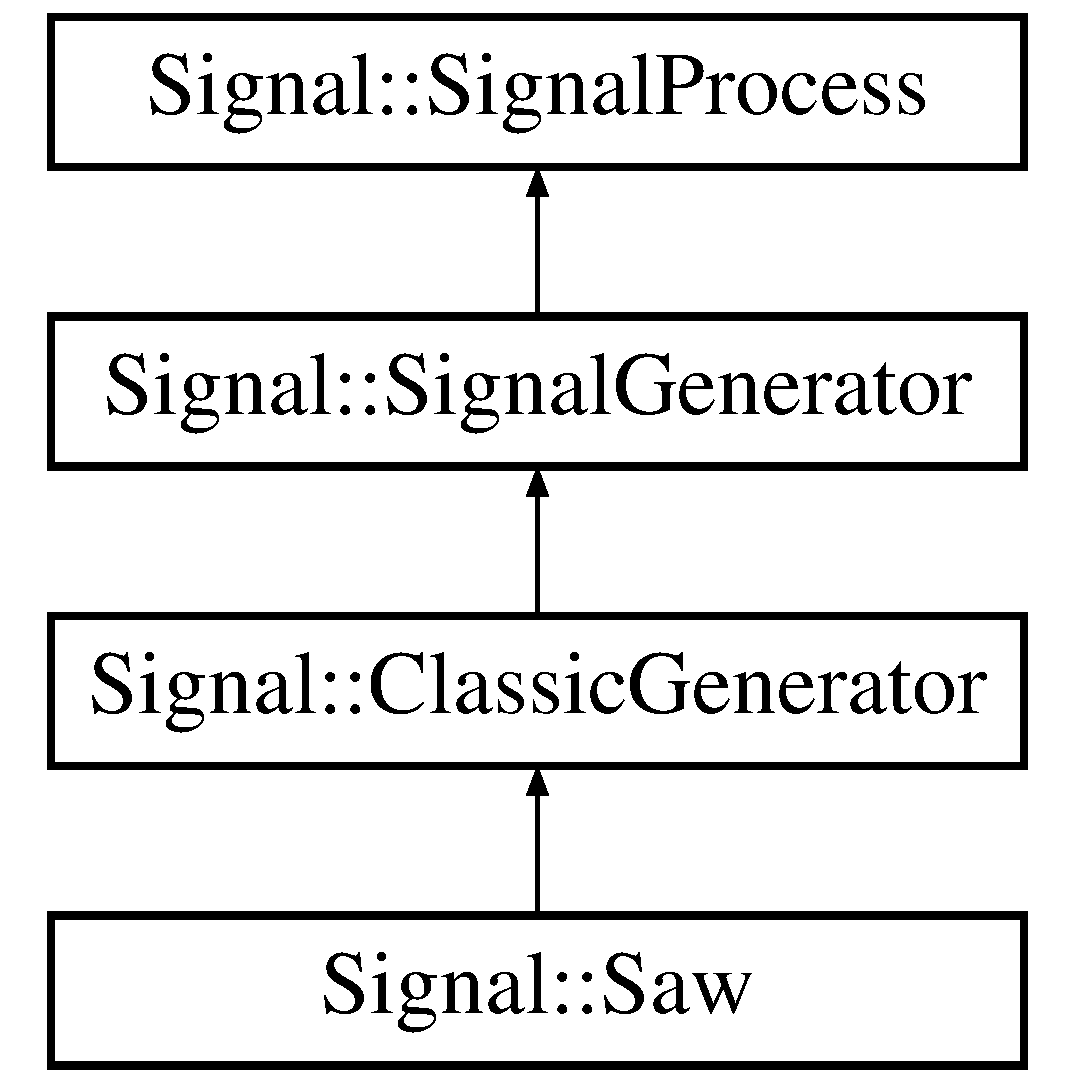
\includegraphics[height=4.000000cm]{classSignal_1_1Saw}
\end{center}
\end{figure}
\subsection*{Public Member Functions}
\begin{DoxyCompactItemize}
\item 
\hyperlink{classSignal_1_1Saw_a4bce6f687d2bd26aa3c2fb209de4c9f9}{Saw} ()
\item 
\hyperlink{classSignal_1_1Saw_a6d772ec845a8c98a4111a7bf1ddabb10}{Saw} (double const \&frequency, double const \&phase\+\_\+offset)
\item 
virtual \hyperlink{classSignal_1_1Saw_a1663e993e22dd1f66033c4de1c1007e9}{$\sim$\+Saw} ()
\item 
virtual bool \hyperlink{classSignal_1_1Saw_a6fb3216b94fea4daa83b27f5de194fa0}{Perform} (\hyperlink{classSignal_1_1Sample}{Sample} \&signal)
\item 
virtual bool \hyperlink{classSignal_1_1Saw_a0d0d374c9b5a3f73f48e9fb1c444b0ca}{Perform} (\hyperlink{classSignal_1_1RingBuffer}{Ring\+Buffer} \&signal)
\item 
virtual double const \& \hyperlink{classSignal_1_1Saw_af91fd0d15b380c02e309705eaad46efd}{Frequency} (double const \&value)
\item 
virtual double const \& \hyperlink{classSignal_1_1Saw_acf3fd0346394d9fd2690bb5fee9550f6}{Frequency} ()
\item 
virtual double const \& \hyperlink{classSignal_1_1SignalGenerator_a96af42ee68f94e9b04d034fd68b73ecd}{Frequency} () const 
\item 
virtual double const \& \hyperlink{classSignal_1_1SignalGenerator_ac2538ec946f001e394d2416fda698d1c}{Phase\+Offset} () const 
\item 
virtual double const \& \hyperlink{classSignal_1_1SignalGenerator_ac6a103ff72beaa338f6d18c812522d78}{Phase\+Offset} (double const \&value)
\end{DoxyCompactItemize}
\subsection*{Protected Member Functions}
\begin{DoxyCompactItemize}
\item 
unsigned long \hyperlink{classSignal_1_1ClassicGenerator_a7457e912d428de4e3fc27ec7fc49890e}{\+\_\+max\+Harms} (double \+\_\+frq)
\item 
double \hyperlink{classSignal_1_1ClassicGenerator_a255330ce8049b6e6d101b8d356cebe3d}{\+\_\+pstep} ()
\item 
double \hyperlink{classSignal_1_1ClassicGenerator_a6571276f584ff0be3862243d0f103a92}{\+\_\+pstep\+\_\+rad} ()
\item 
void \hyperlink{classSignal_1_1ClassicGenerator_a6454565b655bff7b8335735c2fabb4af}{\+\_\+psync} ()
\end{DoxyCompactItemize}
\subsection*{Protected Attributes}
\begin{DoxyCompactItemize}
\item 
unsigned long \hyperlink{classSignal_1_1Saw_a359bfaaab07a3c830da6b81baf045330}{\+\_\+h}
\item 
double \hyperlink{classSignal_1_1Saw_a190de681addc384749845750897859e5}{\+\_\+a}
\item 
double \hyperlink{classSignal_1_1Saw_a96d64ea69f7930c8d7640ecd6944dc84}{phs}
\item 
double \hyperlink{classSignal_1_1Saw_a7c038cabed8c0b51136f16794c9142fd}{stor}
\item 
double \hyperlink{classSignal_1_1Saw_a75052e172f2d3c7ffc8daae2988f7305}{i\+P\+I}
\item 
unsigned short \hyperlink{classSignal_1_1Saw_a50612c8009e428dccb3e4b3b798bdf3d}{i}
\item 
\hyperlink{classSignal_1_1Sample}{Sample} \hyperlink{classSignal_1_1ClassicGenerator_a40313d0d806d6e44af7d41b3ef3a0822}{\+\_\+sample}
\item 
\hyperlink{classSignal_1_1Sample}{Sample} \hyperlink{classSignal_1_1ClassicGenerator_a1214faf589eccb01631700723900bbf9}{\+\_\+storage}
\item 
double \hyperlink{classSignal_1_1ClassicGenerator_ade9b66bc49d2d2f40a1390fc6374b8b2}{\+\_\+phasor}
\item 
double \hyperlink{classSignal_1_1SignalGenerator_a7f107461333bce68c5dad412db96a8c2}{\+\_\+frequency}
\item 
double \hyperlink{classSignal_1_1SignalGenerator_a85a4702347352bab1c71e0a8df8437d6}{\+\_\+f\+Hertz}
\item 
double \hyperlink{classSignal_1_1SignalGenerator_a6b4444d46747c8517171edbbf4b5588f}{\+\_\+phase\+\_\+offset}
\end{DoxyCompactItemize}


\subsection{Detailed Description}


Definition at line 18 of file Saw.\+h.



\subsection{Constructor \& Destructor Documentation}
\hypertarget{classSignal_1_1Saw_a4bce6f687d2bd26aa3c2fb209de4c9f9}{\index{Signal\+::\+Saw@{Signal\+::\+Saw}!Saw@{Saw}}
\index{Saw@{Saw}!Signal\+::\+Saw@{Signal\+::\+Saw}}
\subsubsection[{Saw}]{\setlength{\rightskip}{0pt plus 5cm}Signal\+::\+Saw\+::\+Saw (
\begin{DoxyParamCaption}
{}
\end{DoxyParamCaption}
)}}\label{classSignal_1_1Saw_a4bce6f687d2bd26aa3c2fb209de4c9f9}


Definition at line 10 of file Saw.\+cpp.


\begin{DoxyCode}
10 :\hyperlink{classSignal_1_1ClassicGenerator_a7e4478904de77156deccb1515f6985cb}{ClassicGenerator}(),\hyperlink{classSignal_1_1Saw_a190de681addc384749845750897859e5}{\_a}(5.0/3.0),\hyperlink{classSignal_1_1Saw_a359bfaaab07a3c830da6b81baf045330}{\_h}(\hyperlink{classSignal_1_1ClassicGenerator_a7457e912d428de4e3fc27ec7fc49890e}{\_maxHarms}(
      \hyperlink{classSignal_1_1SignalGenerator_a85a4702347352bab1c71e0a8df8437d6}{\_fHertz})),\hyperlink{classSignal_1_1Saw_a75052e172f2d3c7ffc8daae2988f7305}{iPI}(1.0/\hyperlink{PI_8h_a598a3330b3c21701223ee0ca14316eca}{PI}),\hyperlink{classSignal_1_1Saw_a96d64ea69f7930c8d7640ecd6944dc84}{phs}(0),\hyperlink{classSignal_1_1Saw_a7c038cabed8c0b51136f16794c9142fd}{stor}(0)\{\}
\end{DoxyCode}
\hypertarget{classSignal_1_1Saw_a6d772ec845a8c98a4111a7bf1ddabb10}{\index{Signal\+::\+Saw@{Signal\+::\+Saw}!Saw@{Saw}}
\index{Saw@{Saw}!Signal\+::\+Saw@{Signal\+::\+Saw}}
\subsubsection[{Saw}]{\setlength{\rightskip}{0pt plus 5cm}Signal\+::\+Saw\+::\+Saw (
\begin{DoxyParamCaption}
\item[{double const \&}]{frequency, }
\item[{double const \&}]{phase\+\_\+offset}
\end{DoxyParamCaption}
)}}\label{classSignal_1_1Saw_a6d772ec845a8c98a4111a7bf1ddabb10}


Definition at line 11 of file Saw.\+cpp.


\begin{DoxyCode}
11                                                                 :
      \hyperlink{classSignal_1_1ClassicGenerator_a7e4478904de77156deccb1515f6985cb}{ClassicGenerator}(frequency,phase\_offset),\hyperlink{classSignal_1_1Saw_a190de681addc384749845750897859e5}{\_a}(5.0/3.0),\hyperlink{classSignal_1_1Saw_a359bfaaab07a3c830da6b81baf045330}{\_h}(
      \hyperlink{classSignal_1_1ClassicGenerator_a7457e912d428de4e3fc27ec7fc49890e}{\_maxHarms}(\hyperlink{classSignal_1_1SignalGenerator_a85a4702347352bab1c71e0a8df8437d6}{\_fHertz})),\hyperlink{classSignal_1_1Saw_a75052e172f2d3c7ffc8daae2988f7305}{iPI}(1.0/\hyperlink{PI_8h_a598a3330b3c21701223ee0ca14316eca}{PI}),\hyperlink{classSignal_1_1Saw_a96d64ea69f7930c8d7640ecd6944dc84}{phs}(0),\hyperlink{classSignal_1_1Saw_a7c038cabed8c0b51136f16794c9142fd}{stor}(0)\{
12     \hyperlink{classSignal_1_1ClassicGenerator_a40313d0d806d6e44af7d41b3ef3a0822}{\_sample}=0;
13     \hyperlink{classSignal_1_1ClassicGenerator_a1214faf589eccb01631700723900bbf9}{\_storage}=0;
14 \}
\end{DoxyCode}
\hypertarget{classSignal_1_1Saw_a1663e993e22dd1f66033c4de1c1007e9}{\index{Signal\+::\+Saw@{Signal\+::\+Saw}!````~Saw@{$\sim$\+Saw}}
\index{````~Saw@{$\sim$\+Saw}!Signal\+::\+Saw@{Signal\+::\+Saw}}
\subsubsection[{$\sim$\+Saw}]{\setlength{\rightskip}{0pt plus 5cm}Signal\+::\+Saw\+::$\sim$\+Saw (
\begin{DoxyParamCaption}
{}
\end{DoxyParamCaption}
)\hspace{0.3cm}{\ttfamily [virtual]}}}\label{classSignal_1_1Saw_a1663e993e22dd1f66033c4de1c1007e9}


Definition at line 15 of file Saw.\+cpp.


\begin{DoxyCode}
15 \{\}
\end{DoxyCode}


\subsection{Member Function Documentation}
\hypertarget{classSignal_1_1ClassicGenerator_a7457e912d428de4e3fc27ec7fc49890e}{\index{Signal\+::\+Saw@{Signal\+::\+Saw}!\+\_\+max\+Harms@{\+\_\+max\+Harms}}
\index{\+\_\+max\+Harms@{\+\_\+max\+Harms}!Signal\+::\+Saw@{Signal\+::\+Saw}}
\subsubsection[{\+\_\+max\+Harms}]{\setlength{\rightskip}{0pt plus 5cm}unsigned long Signal\+::\+Classic\+Generator\+::\+\_\+max\+Harms (
\begin{DoxyParamCaption}
\item[{double}]{\+\_\+frq}
\end{DoxyParamCaption}
)\hspace{0.3cm}{\ttfamily [inline]}, {\ttfamily [protected]}, {\ttfamily [inherited]}}}\label{classSignal_1_1ClassicGenerator_a7457e912d428de4e3fc27ec7fc49890e}


Definition at line 70 of file Classic\+Generator.\+h.


\begin{DoxyCode}
70                                                                \{
71         \textcolor{comment}{//double softLim = 0.45;}
72         \textcolor{comment}{//double hardLim = 0.5;}
73         \textcolor{keywordtype}{double} \_s = \hyperlink{namespaceSignal_ae7b1f222afc010e0f33f306f978fcde9}{Sample\_Rate}()* 0.45;
74         \_s/=\_frq;
75         \textcolor{keywordflow}{return} trunc(\_s);
76     \}
\end{DoxyCode}
\hypertarget{classSignal_1_1ClassicGenerator_a255330ce8049b6e6d101b8d356cebe3d}{\index{Signal\+::\+Saw@{Signal\+::\+Saw}!\+\_\+pstep@{\+\_\+pstep}}
\index{\+\_\+pstep@{\+\_\+pstep}!Signal\+::\+Saw@{Signal\+::\+Saw}}
\subsubsection[{\+\_\+pstep}]{\setlength{\rightskip}{0pt plus 5cm}double Signal\+::\+Classic\+Generator\+::\+\_\+pstep (
\begin{DoxyParamCaption}
{}
\end{DoxyParamCaption}
)\hspace{0.3cm}{\ttfamily [inline]}, {\ttfamily [protected]}, {\ttfamily [inherited]}}}\label{classSignal_1_1ClassicGenerator_a255330ce8049b6e6d101b8d356cebe3d}


Definition at line 57 of file Classic\+Generator.\+h.


\begin{DoxyCode}
57                                           \{
58         \textcolor{keywordtype}{double} value = \hyperlink{classSignal_1_1ClassicGenerator_ade9b66bc49d2d2f40a1390fc6374b8b2}{\_phasor};
59         \hyperlink{classSignal_1_1ClassicGenerator_ade9b66bc49d2d2f40a1390fc6374b8b2}{\_phasor}+=\hyperlink{classSignal_1_1SignalGenerator_a7f107461333bce68c5dad412db96a8c2}{\_frequency};
60         \hyperlink{classSignal_1_1ClassicGenerator_ade9b66bc49d2d2f40a1390fc6374b8b2}{\_phasor} = \hyperlink{classSignal_1_1ClassicGenerator_ade9b66bc49d2d2f40a1390fc6374b8b2}{\_phasor}-(\textcolor{keywordtype}{unsigned} long)\hyperlink{classSignal_1_1ClassicGenerator_ade9b66bc49d2d2f40a1390fc6374b8b2}{\_phasor};\textcolor{comment}{//cheaper %1}
61         \textcolor{keywordflow}{return} value;
62     \}
\end{DoxyCode}
\hypertarget{classSignal_1_1ClassicGenerator_a6571276f584ff0be3862243d0f103a92}{\index{Signal\+::\+Saw@{Signal\+::\+Saw}!\+\_\+pstep\+\_\+rad@{\+\_\+pstep\+\_\+rad}}
\index{\+\_\+pstep\+\_\+rad@{\+\_\+pstep\+\_\+rad}!Signal\+::\+Saw@{Signal\+::\+Saw}}
\subsubsection[{\+\_\+pstep\+\_\+rad}]{\setlength{\rightskip}{0pt plus 5cm}double Signal\+::\+Classic\+Generator\+::\+\_\+pstep\+\_\+rad (
\begin{DoxyParamCaption}
{}
\end{DoxyParamCaption}
)\hspace{0.3cm}{\ttfamily [inline]}, {\ttfamily [protected]}, {\ttfamily [inherited]}}}\label{classSignal_1_1ClassicGenerator_a6571276f584ff0be3862243d0f103a92}


Definition at line 63 of file Classic\+Generator.\+h.


\begin{DoxyCode}
63                                               \{
64         \textcolor{keywordflow}{return} \hyperlink{PI_8h_a4912c64aec0c943b7985db6cb61ff83a}{TWOPI} * \hyperlink{classSignal_1_1ClassicGenerator_a255330ce8049b6e6d101b8d356cebe3d}{\_pstep}();
65     \}
\end{DoxyCode}
\hypertarget{classSignal_1_1ClassicGenerator_a6454565b655bff7b8335735c2fabb4af}{\index{Signal\+::\+Saw@{Signal\+::\+Saw}!\+\_\+psync@{\+\_\+psync}}
\index{\+\_\+psync@{\+\_\+psync}!Signal\+::\+Saw@{Signal\+::\+Saw}}
\subsubsection[{\+\_\+psync}]{\setlength{\rightskip}{0pt plus 5cm}void Signal\+::\+Classic\+Generator\+::\+\_\+psync (
\begin{DoxyParamCaption}
{}
\end{DoxyParamCaption}
)\hspace{0.3cm}{\ttfamily [inline]}, {\ttfamily [protected]}, {\ttfamily [inherited]}}}\label{classSignal_1_1ClassicGenerator_a6454565b655bff7b8335735c2fabb4af}


Definition at line 66 of file Classic\+Generator.\+h.


\begin{DoxyCode}
66                                         \{
67         \hyperlink{classSignal_1_1ClassicGenerator_ade9b66bc49d2d2f40a1390fc6374b8b2}{\_phasor} = 0;
68     \}
\end{DoxyCode}
\hypertarget{classSignal_1_1Saw_af91fd0d15b380c02e309705eaad46efd}{\index{Signal\+::\+Saw@{Signal\+::\+Saw}!Frequency@{Frequency}}
\index{Frequency@{Frequency}!Signal\+::\+Saw@{Signal\+::\+Saw}}
\subsubsection[{Frequency}]{\setlength{\rightskip}{0pt plus 5cm}double const \& Signal\+::\+Saw\+::\+Frequency (
\begin{DoxyParamCaption}
\item[{double const \&}]{value}
\end{DoxyParamCaption}
)\hspace{0.3cm}{\ttfamily [virtual]}}}\label{classSignal_1_1Saw_af91fd0d15b380c02e309705eaad46efd}


Reimplemented from \hyperlink{classSignal_1_1SignalGenerator_af83b532bf3ddc3637c2fd7a1dfd095cb}{Signal\+::\+Signal\+Generator}.



Definition at line 16 of file Saw.\+cpp.


\begin{DoxyCode}
16                                                      \{
17     \hyperlink{classSignal_1_1SignalGenerator_a85a4702347352bab1c71e0a8df8437d6}{\_fHertz} = value;
18     \hyperlink{classSignal_1_1SignalGenerator_a7f107461333bce68c5dad412db96a8c2}{\_frequency} = \hyperlink{classSignal_1_1SignalGenerator_a85a4702347352bab1c71e0a8df8437d6}{\_fHertz}/\hyperlink{namespaceSignal_ae7b1f222afc010e0f33f306f978fcde9}{Sample\_Rate}();
19     \hyperlink{classSignal_1_1Saw_a359bfaaab07a3c830da6b81baf045330}{\_h} = \hyperlink{classSignal_1_1ClassicGenerator_a7457e912d428de4e3fc27ec7fc49890e}{\_maxHarms}(\hyperlink{classSignal_1_1SignalGenerator_a85a4702347352bab1c71e0a8df8437d6}{\_fHertz});
20     \textcolor{keywordflow}{return} \hyperlink{classSignal_1_1SignalGenerator_a85a4702347352bab1c71e0a8df8437d6}{\_fHertz};
21 \}
\end{DoxyCode}
\hypertarget{classSignal_1_1Saw_acf3fd0346394d9fd2690bb5fee9550f6}{\index{Signal\+::\+Saw@{Signal\+::\+Saw}!Frequency@{Frequency}}
\index{Frequency@{Frequency}!Signal\+::\+Saw@{Signal\+::\+Saw}}
\subsubsection[{Frequency}]{\setlength{\rightskip}{0pt plus 5cm}double const \& Signal\+::\+Saw\+::\+Frequency (
\begin{DoxyParamCaption}
{}
\end{DoxyParamCaption}
)\hspace{0.3cm}{\ttfamily [virtual]}}}\label{classSignal_1_1Saw_acf3fd0346394d9fd2690bb5fee9550f6}


Definition at line 22 of file Saw.\+cpp.


\begin{DoxyCode}
22                                   \{
23     \textcolor{keywordflow}{return} this->\hyperlink{classSignal_1_1SignalGenerator_a85a4702347352bab1c71e0a8df8437d6}{\_fHertz};
24 \}\end{DoxyCode}
\hypertarget{classSignal_1_1SignalGenerator_a96af42ee68f94e9b04d034fd68b73ecd}{\index{Signal\+::\+Saw@{Signal\+::\+Saw}!Frequency@{Frequency}}
\index{Frequency@{Frequency}!Signal\+::\+Saw@{Signal\+::\+Saw}}
\subsubsection[{Frequency}]{\setlength{\rightskip}{0pt plus 5cm}double const \& Signal\+::\+Signal\+Generator\+::\+Frequency (
\begin{DoxyParamCaption}
{}
\end{DoxyParamCaption}
) const\hspace{0.3cm}{\ttfamily [virtual]}, {\ttfamily [inherited]}}}\label{classSignal_1_1SignalGenerator_a96af42ee68f94e9b04d034fd68b73ecd}


Definition at line 16 of file Signal\+Generator.\+cpp.


\begin{DoxyCode}
16                                                    \{
17     \textcolor{keywordflow}{return} \hyperlink{classSignal_1_1SignalGenerator_a85a4702347352bab1c71e0a8df8437d6}{\_fHertz};
18 \}
\end{DoxyCode}
\hypertarget{classSignal_1_1Saw_a6fb3216b94fea4daa83b27f5de194fa0}{\index{Signal\+::\+Saw@{Signal\+::\+Saw}!Perform@{Perform}}
\index{Perform@{Perform}!Signal\+::\+Saw@{Signal\+::\+Saw}}
\subsubsection[{Perform}]{\setlength{\rightskip}{0pt plus 5cm}bool Signal\+::\+Saw\+::\+Perform (
\begin{DoxyParamCaption}
\item[{{\bf Sample} \&}]{signal}
\end{DoxyParamCaption}
)\hspace{0.3cm}{\ttfamily [inline]}, {\ttfamily [virtual]}}}\label{classSignal_1_1Saw_a6fb3216b94fea4daa83b27f5de194fa0}


Reimplemented from \hyperlink{classSignal_1_1ClassicGenerator_a4a62f329b9cd64d92b07f53c4d593356}{Signal\+::\+Classic\+Generator}.



Definition at line 36 of file Saw.\+h.


\begin{DoxyCode}
36                                           \{
37         \hyperlink{classSignal_1_1Saw_a96d64ea69f7930c8d7640ecd6944dc84}{phs}=\hyperlink{classSignal_1_1ClassicGenerator_a255330ce8049b6e6d101b8d356cebe3d}{\_pstep}();
38         \hyperlink{classSignal_1_1Saw_a96d64ea69f7930c8d7640ecd6944dc84}{phs}+=\hyperlink{classSignal_1_1SignalGenerator_a6b4444d46747c8517171edbbf4b5588f}{\_phase\_offset};
39         signal=0;
40         \textcolor{keywordflow}{for} (\hyperlink{classSignal_1_1Saw_a50612c8009e428dccb3e4b3b798bdf3d}{i}=1; \hyperlink{classSignal_1_1Saw_a50612c8009e428dccb3e4b3b798bdf3d}{i}<\hyperlink{classSignal_1_1Saw_a359bfaaab07a3c830da6b81baf045330}{\_h}+1; ++\hyperlink{classSignal_1_1Saw_a50612c8009e428dccb3e4b3b798bdf3d}{i}) \{
41             \hyperlink{classSignal_1_1Saw_a7c038cabed8c0b51136f16794c9142fd}{stor} += \hyperlink{namespaceSignal_a12e49d2f464a156790c2bdab6db4d28f}{\_harmonicTable}.\hyperlink{classBackend_1_1HarmonicTable_a6b7336f4f6184337350f282d5b0c5467}{Saw}(\hyperlink{classSignal_1_1Saw_a50612c8009e428dccb3e4b3b798bdf3d}{i})* \hyperlink{namespaceSignal_a1ae06d442767e736f514051fcc61d254}{sine}(\hyperlink{classSignal_1_1Saw_a96d64ea69f7930c8d7640ecd6944dc84}{phs}*(
      \hyperlink{classSignal_1_1Saw_a50612c8009e428dccb3e4b3b798bdf3d}{i}));
42         \}
43         \hyperlink{classSignal_1_1Saw_a7c038cabed8c0b51136f16794c9142fd}{stor}*= \hyperlink{classSignal_1_1Saw_a190de681addc384749845750897859e5}{\_a}*\hyperlink{classSignal_1_1Saw_a75052e172f2d3c7ffc8daae2988f7305}{iPI};
44         signal=\hyperlink{classSignal_1_1Saw_a7c038cabed8c0b51136f16794c9142fd}{stor};
45         \textcolor{keywordflow}{return} \textcolor{keyword}{true};
46     \}
\end{DoxyCode}
\hypertarget{classSignal_1_1Saw_a0d0d374c9b5a3f73f48e9fb1c444b0ca}{\index{Signal\+::\+Saw@{Signal\+::\+Saw}!Perform@{Perform}}
\index{Perform@{Perform}!Signal\+::\+Saw@{Signal\+::\+Saw}}
\subsubsection[{Perform}]{\setlength{\rightskip}{0pt plus 5cm}bool Signal\+::\+Saw\+::\+Perform (
\begin{DoxyParamCaption}
\item[{{\bf Ring\+Buffer} \&}]{signal}
\end{DoxyParamCaption}
)\hspace{0.3cm}{\ttfamily [inline]}, {\ttfamily [virtual]}}}\label{classSignal_1_1Saw_a0d0d374c9b5a3f73f48e9fb1c444b0ca}


Reimplemented from \hyperlink{classSignal_1_1ClassicGenerator_a308c13baa66020d44c2227bd58db4b4f}{Signal\+::\+Classic\+Generator}.



Definition at line 47 of file Saw.\+h.


\begin{DoxyCode}
47                                               \{
48         signal.Flush();
49         \textcolor{keywordflow}{while} (!signal.Full()) \{
50             \textcolor{keywordflow}{if} (\hyperlink{classSignal_1_1Saw_a6fb3216b94fea4daa83b27f5de194fa0}{Perform}(\hyperlink{classSignal_1_1ClassicGenerator_a40313d0d806d6e44af7d41b3ef3a0822}{\_sample})) \{
51                 \textcolor{keywordflow}{if}(signal.Write(\hyperlink{classSignal_1_1ClassicGenerator_a40313d0d806d6e44af7d41b3ef3a0822}{\_sample}))\{
52                 \}\textcolor{keywordflow}{else} \textcolor{keywordflow}{return} \textcolor{keyword}{false};
53             \}\textcolor{keywordflow}{else} \textcolor{keywordflow}{return} \textcolor{keyword}{false};
54         \}\textcolor{keywordflow}{return} \textcolor{keyword}{true};
55     \}
\end{DoxyCode}
\hypertarget{classSignal_1_1SignalGenerator_ac2538ec946f001e394d2416fda698d1c}{\index{Signal\+::\+Saw@{Signal\+::\+Saw}!Phase\+Offset@{Phase\+Offset}}
\index{Phase\+Offset@{Phase\+Offset}!Signal\+::\+Saw@{Signal\+::\+Saw}}
\subsubsection[{Phase\+Offset}]{\setlength{\rightskip}{0pt plus 5cm}double const \& Signal\+::\+Signal\+Generator\+::\+Phase\+Offset (
\begin{DoxyParamCaption}
{}
\end{DoxyParamCaption}
) const\hspace{0.3cm}{\ttfamily [virtual]}, {\ttfamily [inherited]}}}\label{classSignal_1_1SignalGenerator_ac2538ec946f001e394d2416fda698d1c}


Definition at line 24 of file Signal\+Generator.\+cpp.


\begin{DoxyCode}
24                                                      \{
25     \textcolor{keywordflow}{return} \hyperlink{classSignal_1_1SignalGenerator_a6b4444d46747c8517171edbbf4b5588f}{\_phase\_offset};
26 \}
\end{DoxyCode}
\hypertarget{classSignal_1_1SignalGenerator_ac6a103ff72beaa338f6d18c812522d78}{\index{Signal\+::\+Saw@{Signal\+::\+Saw}!Phase\+Offset@{Phase\+Offset}}
\index{Phase\+Offset@{Phase\+Offset}!Signal\+::\+Saw@{Signal\+::\+Saw}}
\subsubsection[{Phase\+Offset}]{\setlength{\rightskip}{0pt plus 5cm}double const \& Signal\+::\+Signal\+Generator\+::\+Phase\+Offset (
\begin{DoxyParamCaption}
\item[{double const \&}]{value}
\end{DoxyParamCaption}
)\hspace{0.3cm}{\ttfamily [virtual]}, {\ttfamily [inherited]}}}\label{classSignal_1_1SignalGenerator_ac6a103ff72beaa338f6d18c812522d78}


Definition at line 27 of file Signal\+Generator.\+cpp.


\begin{DoxyCode}
27                                                                    \{
28     \hyperlink{classSignal_1_1SignalGenerator_a6b4444d46747c8517171edbbf4b5588f}{\_phase\_offset} = value;
29     \textcolor{keywordflow}{return} \hyperlink{classSignal_1_1SignalGenerator_a6b4444d46747c8517171edbbf4b5588f}{\_phase\_offset};
30 \}
\end{DoxyCode}


\subsection{Member Data Documentation}
\hypertarget{classSignal_1_1Saw_a190de681addc384749845750897859e5}{\index{Signal\+::\+Saw@{Signal\+::\+Saw}!\+\_\+a@{\+\_\+a}}
\index{\+\_\+a@{\+\_\+a}!Signal\+::\+Saw@{Signal\+::\+Saw}}
\subsubsection[{\+\_\+a}]{\setlength{\rightskip}{0pt plus 5cm}double Signal\+::\+Saw\+::\+\_\+a\hspace{0.3cm}{\ttfamily [protected]}}}\label{classSignal_1_1Saw_a190de681addc384749845750897859e5}


Definition at line 29 of file Saw.\+h.

\hypertarget{classSignal_1_1SignalGenerator_a85a4702347352bab1c71e0a8df8437d6}{\index{Signal\+::\+Saw@{Signal\+::\+Saw}!\+\_\+f\+Hertz@{\+\_\+f\+Hertz}}
\index{\+\_\+f\+Hertz@{\+\_\+f\+Hertz}!Signal\+::\+Saw@{Signal\+::\+Saw}}
\subsubsection[{\+\_\+f\+Hertz}]{\setlength{\rightskip}{0pt plus 5cm}double Signal\+::\+Signal\+Generator\+::\+\_\+f\+Hertz\hspace{0.3cm}{\ttfamily [protected]}, {\ttfamily [inherited]}}}\label{classSignal_1_1SignalGenerator_a85a4702347352bab1c71e0a8df8437d6}


Definition at line 34 of file Signal\+Generator.\+h.

\hypertarget{classSignal_1_1SignalGenerator_a7f107461333bce68c5dad412db96a8c2}{\index{Signal\+::\+Saw@{Signal\+::\+Saw}!\+\_\+frequency@{\+\_\+frequency}}
\index{\+\_\+frequency@{\+\_\+frequency}!Signal\+::\+Saw@{Signal\+::\+Saw}}
\subsubsection[{\+\_\+frequency}]{\setlength{\rightskip}{0pt plus 5cm}double Signal\+::\+Signal\+Generator\+::\+\_\+frequency\hspace{0.3cm}{\ttfamily [protected]}, {\ttfamily [inherited]}}}\label{classSignal_1_1SignalGenerator_a7f107461333bce68c5dad412db96a8c2}


Definition at line 33 of file Signal\+Generator.\+h.

\hypertarget{classSignal_1_1Saw_a359bfaaab07a3c830da6b81baf045330}{\index{Signal\+::\+Saw@{Signal\+::\+Saw}!\+\_\+h@{\+\_\+h}}
\index{\+\_\+h@{\+\_\+h}!Signal\+::\+Saw@{Signal\+::\+Saw}}
\subsubsection[{\+\_\+h}]{\setlength{\rightskip}{0pt plus 5cm}unsigned long Signal\+::\+Saw\+::\+\_\+h\hspace{0.3cm}{\ttfamily [protected]}}}\label{classSignal_1_1Saw_a359bfaaab07a3c830da6b81baf045330}


Definition at line 28 of file Saw.\+h.

\hypertarget{classSignal_1_1SignalGenerator_a6b4444d46747c8517171edbbf4b5588f}{\index{Signal\+::\+Saw@{Signal\+::\+Saw}!\+\_\+phase\+\_\+offset@{\+\_\+phase\+\_\+offset}}
\index{\+\_\+phase\+\_\+offset@{\+\_\+phase\+\_\+offset}!Signal\+::\+Saw@{Signal\+::\+Saw}}
\subsubsection[{\+\_\+phase\+\_\+offset}]{\setlength{\rightskip}{0pt plus 5cm}double Signal\+::\+Signal\+Generator\+::\+\_\+phase\+\_\+offset\hspace{0.3cm}{\ttfamily [protected]}, {\ttfamily [inherited]}}}\label{classSignal_1_1SignalGenerator_a6b4444d46747c8517171edbbf4b5588f}


Definition at line 35 of file Signal\+Generator.\+h.

\hypertarget{classSignal_1_1ClassicGenerator_ade9b66bc49d2d2f40a1390fc6374b8b2}{\index{Signal\+::\+Saw@{Signal\+::\+Saw}!\+\_\+phasor@{\+\_\+phasor}}
\index{\+\_\+phasor@{\+\_\+phasor}!Signal\+::\+Saw@{Signal\+::\+Saw}}
\subsubsection[{\+\_\+phasor}]{\setlength{\rightskip}{0pt plus 5cm}double Signal\+::\+Classic\+Generator\+::\+\_\+phasor\hspace{0.3cm}{\ttfamily [protected]}, {\ttfamily [inherited]}}}\label{classSignal_1_1ClassicGenerator_ade9b66bc49d2d2f40a1390fc6374b8b2}


Definition at line 41 of file Classic\+Generator.\+h.

\hypertarget{classSignal_1_1ClassicGenerator_a40313d0d806d6e44af7d41b3ef3a0822}{\index{Signal\+::\+Saw@{Signal\+::\+Saw}!\+\_\+sample@{\+\_\+sample}}
\index{\+\_\+sample@{\+\_\+sample}!Signal\+::\+Saw@{Signal\+::\+Saw}}
\subsubsection[{\+\_\+sample}]{\setlength{\rightskip}{0pt plus 5cm}{\bf Sample} Signal\+::\+Classic\+Generator\+::\+\_\+sample\hspace{0.3cm}{\ttfamily [protected]}, {\ttfamily [inherited]}}}\label{classSignal_1_1ClassicGenerator_a40313d0d806d6e44af7d41b3ef3a0822}


Definition at line 34 of file Classic\+Generator.\+h.

\hypertarget{classSignal_1_1ClassicGenerator_a1214faf589eccb01631700723900bbf9}{\index{Signal\+::\+Saw@{Signal\+::\+Saw}!\+\_\+storage@{\+\_\+storage}}
\index{\+\_\+storage@{\+\_\+storage}!Signal\+::\+Saw@{Signal\+::\+Saw}}
\subsubsection[{\+\_\+storage}]{\setlength{\rightskip}{0pt plus 5cm}{\bf Sample} Signal\+::\+Classic\+Generator\+::\+\_\+storage\hspace{0.3cm}{\ttfamily [protected]}, {\ttfamily [inherited]}}}\label{classSignal_1_1ClassicGenerator_a1214faf589eccb01631700723900bbf9}


Definition at line 35 of file Classic\+Generator.\+h.

\hypertarget{classSignal_1_1Saw_a50612c8009e428dccb3e4b3b798bdf3d}{\index{Signal\+::\+Saw@{Signal\+::\+Saw}!i@{i}}
\index{i@{i}!Signal\+::\+Saw@{Signal\+::\+Saw}}
\subsubsection[{i}]{\setlength{\rightskip}{0pt plus 5cm}unsigned short Signal\+::\+Saw\+::i\hspace{0.3cm}{\ttfamily [protected]}}}\label{classSignal_1_1Saw_a50612c8009e428dccb3e4b3b798bdf3d}


Definition at line 33 of file Saw.\+h.

\hypertarget{classSignal_1_1Saw_a75052e172f2d3c7ffc8daae2988f7305}{\index{Signal\+::\+Saw@{Signal\+::\+Saw}!i\+P\+I@{i\+P\+I}}
\index{i\+P\+I@{i\+P\+I}!Signal\+::\+Saw@{Signal\+::\+Saw}}
\subsubsection[{i\+P\+I}]{\setlength{\rightskip}{0pt plus 5cm}double Signal\+::\+Saw\+::i\+P\+I\hspace{0.3cm}{\ttfamily [protected]}}}\label{classSignal_1_1Saw_a75052e172f2d3c7ffc8daae2988f7305}


Definition at line 32 of file Saw.\+h.

\hypertarget{classSignal_1_1Saw_a96d64ea69f7930c8d7640ecd6944dc84}{\index{Signal\+::\+Saw@{Signal\+::\+Saw}!phs@{phs}}
\index{phs@{phs}!Signal\+::\+Saw@{Signal\+::\+Saw}}
\subsubsection[{phs}]{\setlength{\rightskip}{0pt plus 5cm}double Signal\+::\+Saw\+::phs\hspace{0.3cm}{\ttfamily [protected]}}}\label{classSignal_1_1Saw_a96d64ea69f7930c8d7640ecd6944dc84}


Definition at line 30 of file Saw.\+h.

\hypertarget{classSignal_1_1Saw_a7c038cabed8c0b51136f16794c9142fd}{\index{Signal\+::\+Saw@{Signal\+::\+Saw}!stor@{stor}}
\index{stor@{stor}!Signal\+::\+Saw@{Signal\+::\+Saw}}
\subsubsection[{stor}]{\setlength{\rightskip}{0pt plus 5cm}double Signal\+::\+Saw\+::stor\hspace{0.3cm}{\ttfamily [protected]}}}\label{classSignal_1_1Saw_a7c038cabed8c0b51136f16794c9142fd}


Definition at line 31 of file Saw.\+h.



The documentation for this class was generated from the following files\+:\begin{DoxyCompactItemize}
\item 
/\+Users/alexanderzywicki/\+Documents/\+School\+\_\+\+Stuff/\+Fall\+\_\+2014/\+Digital\+\_\+\+Signal\+\_\+\+Generation\+\_\+and\+\_\+\+Analysis/src/include/\hyperlink{Saw_8h}{Saw.\+h}\item 
/\+Users/alexanderzywicki/\+Documents/\+School\+\_\+\+Stuff/\+Fall\+\_\+2014/\+Digital\+\_\+\+Signal\+\_\+\+Generation\+\_\+and\+\_\+\+Analysis/src/\hyperlink{Saw_8cpp}{Saw.\+cpp}\end{DoxyCompactItemize}

\hypertarget{classSignal_1_1SignalGenerator}{\section{Signal\+:\+:Signal\+Generator Class Reference}
\label{classSignal_1_1SignalGenerator}\index{Signal\+::\+Signal\+Generator@{Signal\+::\+Signal\+Generator}}
}


{\ttfamily \#include $<$Signal\+Generator.\+h$>$}

Inheritance diagram for Signal\+:\+:Signal\+Generator\+:\begin{figure}[H]
\begin{center}
\leavevmode
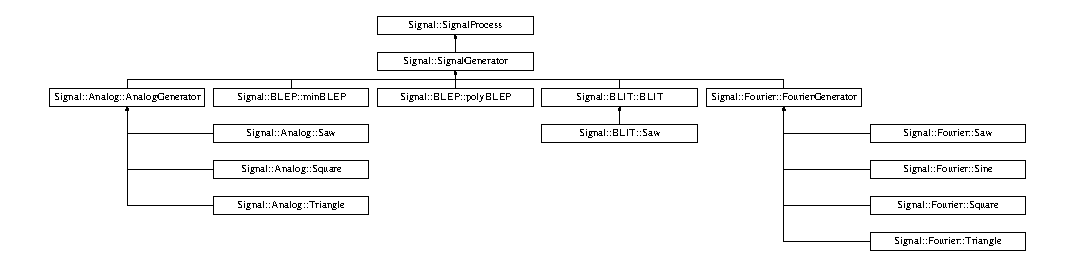
\includegraphics[height=1.346154cm]{classSignal_1_1SignalGenerator}
\end{center}
\end{figure}
\subsection*{Public Member Functions}
\begin{DoxyCompactItemize}
\item 
\hyperlink{classSignal_1_1SignalGenerator_a8c67c754d86e0363445d7fd271855e1a}{Signal\+Generator} ()
\item 
\hyperlink{classSignal_1_1SignalGenerator_a0a09e58b391b2e65af370bbf266b888c}{Signal\+Generator} (double const \&frequency, double const \&phase\+\_\+offset)
\item 
virtual \hyperlink{classSignal_1_1SignalGenerator_a2c0cb5fa941326bc206f45a07aa872ef}{$\sim$\+Signal\+Generator} ()
\item 
virtual bool \hyperlink{classSignal_1_1SignalGenerator_a2cd9061c5ae40a392a9476551b4379f3}{Perform} (\hyperlink{classSignal_1_1Sample}{Sample} \&signal)
\item 
virtual bool \hyperlink{classSignal_1_1SignalGenerator_a126d52dd9b6b14d33efc624e2c89284e}{Perform} (\hyperlink{classSignal_1_1RingBuffer}{Ring\+Buffer} \&signal)
\item 
virtual double const \& \hyperlink{classSignal_1_1SignalGenerator_a96af42ee68f94e9b04d034fd68b73ecd}{Frequency} () const 
\item 
virtual double const \& \hyperlink{classSignal_1_1SignalGenerator_af83b532bf3ddc3637c2fd7a1dfd095cb}{Frequency} (double const \&value)
\item 
virtual double const \& \hyperlink{classSignal_1_1SignalGenerator_ac2538ec946f001e394d2416fda698d1c}{Phase\+Offset} () const 
\item 
virtual double const \& \hyperlink{classSignal_1_1SignalGenerator_ac6a103ff72beaa338f6d18c812522d78}{Phase\+Offset} (double const \&value)
\end{DoxyCompactItemize}
\subsection*{Protected Attributes}
\begin{DoxyCompactItemize}
\item 
double \hyperlink{classSignal_1_1SignalGenerator_a7f107461333bce68c5dad412db96a8c2}{\+\_\+frequency}
\item 
double \hyperlink{classSignal_1_1SignalGenerator_a85a4702347352bab1c71e0a8df8437d6}{\+\_\+f\+Hertz}
\item 
double \hyperlink{classSignal_1_1SignalGenerator_a6b4444d46747c8517171edbbf4b5588f}{\+\_\+phase\+\_\+offset}
\end{DoxyCompactItemize}


\subsection{Detailed Description}


Definition at line 19 of file Signal\+Generator.\+h.



\subsection{Constructor \& Destructor Documentation}
\hypertarget{classSignal_1_1SignalGenerator_a8c67c754d86e0363445d7fd271855e1a}{\index{Signal\+::\+Signal\+Generator@{Signal\+::\+Signal\+Generator}!Signal\+Generator@{Signal\+Generator}}
\index{Signal\+Generator@{Signal\+Generator}!Signal\+::\+Signal\+Generator@{Signal\+::\+Signal\+Generator}}
\subsubsection[{Signal\+Generator}]{\setlength{\rightskip}{0pt plus 5cm}Signal\+::\+Signal\+Generator\+::\+Signal\+Generator (
\begin{DoxyParamCaption}
{}
\end{DoxyParamCaption}
)}}\label{classSignal_1_1SignalGenerator_a8c67c754d86e0363445d7fd271855e1a}


Definition at line 10 of file Signal\+Generator.\+cpp.


\begin{DoxyCode}
10                                       :\hyperlink{classSignal_1_1SignalGenerator_a7f107461333bce68c5dad412db96a8c2}{\_frequency}(0),\hyperlink{classSignal_1_1SignalGenerator_a6b4444d46747c8517171edbbf4b5588f}{\_phase\_offset}(0),
      \hyperlink{classSignal_1_1SignalGenerator_a85a4702347352bab1c71e0a8df8437d6}{\_fHertz}(0)\{
11 
12 \}
\end{DoxyCode}
\hypertarget{classSignal_1_1SignalGenerator_a0a09e58b391b2e65af370bbf266b888c}{\index{Signal\+::\+Signal\+Generator@{Signal\+::\+Signal\+Generator}!Signal\+Generator@{Signal\+Generator}}
\index{Signal\+Generator@{Signal\+Generator}!Signal\+::\+Signal\+Generator@{Signal\+::\+Signal\+Generator}}
\subsubsection[{Signal\+Generator}]{\setlength{\rightskip}{0pt plus 5cm}Signal\+::\+Signal\+Generator\+::\+Signal\+Generator (
\begin{DoxyParamCaption}
\item[{double const \&}]{frequency, }
\item[{double const \&}]{phase\+\_\+offset}
\end{DoxyParamCaption}
)}}\label{classSignal_1_1SignalGenerator_a0a09e58b391b2e65af370bbf266b888c}


Definition at line 13 of file Signal\+Generator.\+cpp.


\begin{DoxyCode}
13 :\hyperlink{classSignal_1_1SignalGenerator_a7f107461333bce68c5dad412db96a8c2}{\_frequency}(frequency/\hyperlink{namespaceSignal_ae7b1f222afc010e0f33f306f978fcde9}{Sample\_Rate}()),\hyperlink{classSignal_1_1SignalGenerator_a85a4702347352bab1c71e0a8df8437d6}{\_fHertz}(frequency),
      \hyperlink{classSignal_1_1SignalGenerator_a6b4444d46747c8517171edbbf4b5588f}{\_phase\_offset}(phase\_offset)\{\}
\end{DoxyCode}
\hypertarget{classSignal_1_1SignalGenerator_a2c0cb5fa941326bc206f45a07aa872ef}{\index{Signal\+::\+Signal\+Generator@{Signal\+::\+Signal\+Generator}!````~Signal\+Generator@{$\sim$\+Signal\+Generator}}
\index{````~Signal\+Generator@{$\sim$\+Signal\+Generator}!Signal\+::\+Signal\+Generator@{Signal\+::\+Signal\+Generator}}
\subsubsection[{$\sim$\+Signal\+Generator}]{\setlength{\rightskip}{0pt plus 5cm}Signal\+::\+Signal\+Generator\+::$\sim$\+Signal\+Generator (
\begin{DoxyParamCaption}
{}
\end{DoxyParamCaption}
)\hspace{0.3cm}{\ttfamily [virtual]}}}\label{classSignal_1_1SignalGenerator_a2c0cb5fa941326bc206f45a07aa872ef}


Definition at line 14 of file Signal\+Generator.\+cpp.


\begin{DoxyCode}
14 \{\}
\end{DoxyCode}


\subsection{Member Function Documentation}
\hypertarget{classSignal_1_1SignalGenerator_a96af42ee68f94e9b04d034fd68b73ecd}{\index{Signal\+::\+Signal\+Generator@{Signal\+::\+Signal\+Generator}!Frequency@{Frequency}}
\index{Frequency@{Frequency}!Signal\+::\+Signal\+Generator@{Signal\+::\+Signal\+Generator}}
\subsubsection[{Frequency}]{\setlength{\rightskip}{0pt plus 5cm}double const \& Signal\+::\+Signal\+Generator\+::\+Frequency (
\begin{DoxyParamCaption}
{}
\end{DoxyParamCaption}
) const\hspace{0.3cm}{\ttfamily [virtual]}}}\label{classSignal_1_1SignalGenerator_a96af42ee68f94e9b04d034fd68b73ecd}


Definition at line 16 of file Signal\+Generator.\+cpp.


\begin{DoxyCode}
16                                                    \{
17     \textcolor{keywordflow}{return} \hyperlink{classSignal_1_1SignalGenerator_a85a4702347352bab1c71e0a8df8437d6}{\_fHertz};
18 \}
\end{DoxyCode}
\hypertarget{classSignal_1_1SignalGenerator_af83b532bf3ddc3637c2fd7a1dfd095cb}{\index{Signal\+::\+Signal\+Generator@{Signal\+::\+Signal\+Generator}!Frequency@{Frequency}}
\index{Frequency@{Frequency}!Signal\+::\+Signal\+Generator@{Signal\+::\+Signal\+Generator}}
\subsubsection[{Frequency}]{\setlength{\rightskip}{0pt plus 5cm}double const \& Signal\+::\+Signal\+Generator\+::\+Frequency (
\begin{DoxyParamCaption}
\item[{double const \&}]{value}
\end{DoxyParamCaption}
)\hspace{0.3cm}{\ttfamily [virtual]}}}\label{classSignal_1_1SignalGenerator_af83b532bf3ddc3637c2fd7a1dfd095cb}


Reimplemented in \hyperlink{classSignal_1_1BLIT_1_1BLIT_a59110620478308054d4c932c613e5cc6}{Signal\+::\+B\+L\+I\+T\+::\+B\+L\+I\+T}, \hyperlink{classSignal_1_1Fourier_1_1Saw_a398a26142f42cdc5cb33230e9ab05b9d}{Signal\+::\+Fourier\+::\+Saw}, and \hyperlink{classSignal_1_1Fourier_1_1Square_a99040022c5d7c9f88e52cdeeed3e797a}{Signal\+::\+Fourier\+::\+Square}.



Definition at line 19 of file Signal\+Generator.\+cpp.


\begin{DoxyCode}
19                                                                  \{
20     \hyperlink{classSignal_1_1SignalGenerator_a85a4702347352bab1c71e0a8df8437d6}{\_fHertz} = value;
21     \hyperlink{classSignal_1_1SignalGenerator_a7f107461333bce68c5dad412db96a8c2}{\_frequency} = \hyperlink{classSignal_1_1SignalGenerator_a85a4702347352bab1c71e0a8df8437d6}{\_fHertz}/\hyperlink{namespaceSignal_ae7b1f222afc010e0f33f306f978fcde9}{Sample\_Rate}();
22     \textcolor{keywordflow}{return} \hyperlink{classSignal_1_1SignalGenerator_a85a4702347352bab1c71e0a8df8437d6}{\_fHertz};
23 \}
\end{DoxyCode}
\hypertarget{classSignal_1_1SignalGenerator_a2cd9061c5ae40a392a9476551b4379f3}{\index{Signal\+::\+Signal\+Generator@{Signal\+::\+Signal\+Generator}!Perform@{Perform}}
\index{Perform@{Perform}!Signal\+::\+Signal\+Generator@{Signal\+::\+Signal\+Generator}}
\subsubsection[{Perform}]{\setlength{\rightskip}{0pt plus 5cm}bool Signal\+::\+Signal\+Generator\+::\+Perform (
\begin{DoxyParamCaption}
\item[{{\bf Sample} \&}]{signal}
\end{DoxyParamCaption}
)\hspace{0.3cm}{\ttfamily [inline]}, {\ttfamily [virtual]}}}\label{classSignal_1_1SignalGenerator_a2cd9061c5ae40a392a9476551b4379f3}


Implements \hyperlink{classSignal_1_1SignalProcess_a7986df989ac8afca3674ae8eace3cfdb}{Signal\+::\+Signal\+Process}.



Reimplemented in \hyperlink{classSignal_1_1Fourier_1_1Sine_aa35c77904f8d7a0de6fa4895d6c53644}{Signal\+::\+Fourier\+::\+Sine}, \hyperlink{classSignal_1_1Fourier_1_1FourierGenerator_a6ec444e7b66d2cb339c001704071646a}{Signal\+::\+Fourier\+::\+Fourier\+Generator}, \hyperlink{classSignal_1_1BLIT_1_1BLIT_a98982b34bc6c9ca4c2e91550afa31375}{Signal\+::\+B\+L\+I\+T\+::\+B\+L\+I\+T}, \hyperlink{classSignal_1_1Trivial_1_1TrivialGenerator_a2394cf9d0d40f9d25f72aff03e372ad9}{Signal\+::\+Trivial\+::\+Trivial\+Generator}, \hyperlink{classSignal_1_1Fourier_1_1Saw_adf69eea95516fc9c7d06fae036d2fa9b}{Signal\+::\+Fourier\+::\+Saw}, \hyperlink{classSignal_1_1Fourier_1_1Square_a29e4b9d03b9df4fb6ed0d7a817ecffda}{Signal\+::\+Fourier\+::\+Square}, and \hyperlink{classSignal_1_1Trivial_1_1TrivialSaw_a091e3137a03978cc7dfaecf5b00dad46}{Signal\+::\+Trivial\+::\+Trivial\+Saw}.



Definition at line 39 of file Signal\+Generator.\+h.


\begin{DoxyCode}
39                                                       \{
40         signal = 0;
41         \textcolor{keywordflow}{return} \textcolor{keyword}{false};
42     \}
\end{DoxyCode}
\hypertarget{classSignal_1_1SignalGenerator_a126d52dd9b6b14d33efc624e2c89284e}{\index{Signal\+::\+Signal\+Generator@{Signal\+::\+Signal\+Generator}!Perform@{Perform}}
\index{Perform@{Perform}!Signal\+::\+Signal\+Generator@{Signal\+::\+Signal\+Generator}}
\subsubsection[{Perform}]{\setlength{\rightskip}{0pt plus 5cm}bool Signal\+::\+Signal\+Generator\+::\+Perform (
\begin{DoxyParamCaption}
\item[{{\bf Ring\+Buffer} \&}]{signal}
\end{DoxyParamCaption}
)\hspace{0.3cm}{\ttfamily [inline]}, {\ttfamily [virtual]}}}\label{classSignal_1_1SignalGenerator_a126d52dd9b6b14d33efc624e2c89284e}


Implements \hyperlink{classSignal_1_1SignalProcess_a9584dc515d2167f4439ed3d014bbb3f7}{Signal\+::\+Signal\+Process}.



Reimplemented in \hyperlink{classSignal_1_1Fourier_1_1Sine_a5d951e5fbfc77354bddab9dfedea008f}{Signal\+::\+Fourier\+::\+Sine}, \hyperlink{classSignal_1_1Fourier_1_1FourierGenerator_acc6a3825eb4060269749a37ae29ee847}{Signal\+::\+Fourier\+::\+Fourier\+Generator}, \hyperlink{classSignal_1_1BLIT_1_1BLIT_a2f0ee604ed0e67557aa9f7e7f50d80ec}{Signal\+::\+B\+L\+I\+T\+::\+B\+L\+I\+T}, \hyperlink{classSignal_1_1Trivial_1_1TrivialGenerator_a232aefbb2815eaf25e697ecedeb0f3d9}{Signal\+::\+Trivial\+::\+Trivial\+Generator}, \hyperlink{classSignal_1_1Fourier_1_1Saw_acef099db2217902d7157e5b93f658363}{Signal\+::\+Fourier\+::\+Saw}, \hyperlink{classSignal_1_1Fourier_1_1Square_a7aacafda4427b996b56ad6764ea09177}{Signal\+::\+Fourier\+::\+Square}, and \hyperlink{classSignal_1_1Trivial_1_1TrivialSaw_a22b97c8dfdca76664cbb6e634c85085d}{Signal\+::\+Trivial\+::\+Trivial\+Saw}.



Definition at line 43 of file Signal\+Generator.\+h.


\begin{DoxyCode}
43                                                           \{
44         signal.Flush();
45         \textcolor{keywordflow}{return} \textcolor{keyword}{false};
46     \}
\end{DoxyCode}
\hypertarget{classSignal_1_1SignalGenerator_ac2538ec946f001e394d2416fda698d1c}{\index{Signal\+::\+Signal\+Generator@{Signal\+::\+Signal\+Generator}!Phase\+Offset@{Phase\+Offset}}
\index{Phase\+Offset@{Phase\+Offset}!Signal\+::\+Signal\+Generator@{Signal\+::\+Signal\+Generator}}
\subsubsection[{Phase\+Offset}]{\setlength{\rightskip}{0pt plus 5cm}double const \& Signal\+::\+Signal\+Generator\+::\+Phase\+Offset (
\begin{DoxyParamCaption}
{}
\end{DoxyParamCaption}
) const\hspace{0.3cm}{\ttfamily [virtual]}}}\label{classSignal_1_1SignalGenerator_ac2538ec946f001e394d2416fda698d1c}


Definition at line 24 of file Signal\+Generator.\+cpp.


\begin{DoxyCode}
24                                                      \{
25     \textcolor{keywordflow}{return} \hyperlink{classSignal_1_1SignalGenerator_a6b4444d46747c8517171edbbf4b5588f}{\_phase\_offset};
26 \}
\end{DoxyCode}
\hypertarget{classSignal_1_1SignalGenerator_ac6a103ff72beaa338f6d18c812522d78}{\index{Signal\+::\+Signal\+Generator@{Signal\+::\+Signal\+Generator}!Phase\+Offset@{Phase\+Offset}}
\index{Phase\+Offset@{Phase\+Offset}!Signal\+::\+Signal\+Generator@{Signal\+::\+Signal\+Generator}}
\subsubsection[{Phase\+Offset}]{\setlength{\rightskip}{0pt plus 5cm}double const \& Signal\+::\+Signal\+Generator\+::\+Phase\+Offset (
\begin{DoxyParamCaption}
\item[{double const \&}]{value}
\end{DoxyParamCaption}
)\hspace{0.3cm}{\ttfamily [virtual]}}}\label{classSignal_1_1SignalGenerator_ac6a103ff72beaa338f6d18c812522d78}


Definition at line 27 of file Signal\+Generator.\+cpp.


\begin{DoxyCode}
27                                                                    \{
28     \hyperlink{classSignal_1_1SignalGenerator_a6b4444d46747c8517171edbbf4b5588f}{\_phase\_offset} = value;
29     \textcolor{keywordflow}{return} \hyperlink{classSignal_1_1SignalGenerator_a6b4444d46747c8517171edbbf4b5588f}{\_phase\_offset};
30 \}
\end{DoxyCode}


\subsection{Member Data Documentation}
\hypertarget{classSignal_1_1SignalGenerator_a85a4702347352bab1c71e0a8df8437d6}{\index{Signal\+::\+Signal\+Generator@{Signal\+::\+Signal\+Generator}!\+\_\+f\+Hertz@{\+\_\+f\+Hertz}}
\index{\+\_\+f\+Hertz@{\+\_\+f\+Hertz}!Signal\+::\+Signal\+Generator@{Signal\+::\+Signal\+Generator}}
\subsubsection[{\+\_\+f\+Hertz}]{\setlength{\rightskip}{0pt plus 5cm}double Signal\+::\+Signal\+Generator\+::\+\_\+f\+Hertz\hspace{0.3cm}{\ttfamily [protected]}}}\label{classSignal_1_1SignalGenerator_a85a4702347352bab1c71e0a8df8437d6}


Definition at line 34 of file Signal\+Generator.\+h.

\hypertarget{classSignal_1_1SignalGenerator_a7f107461333bce68c5dad412db96a8c2}{\index{Signal\+::\+Signal\+Generator@{Signal\+::\+Signal\+Generator}!\+\_\+frequency@{\+\_\+frequency}}
\index{\+\_\+frequency@{\+\_\+frequency}!Signal\+::\+Signal\+Generator@{Signal\+::\+Signal\+Generator}}
\subsubsection[{\+\_\+frequency}]{\setlength{\rightskip}{0pt plus 5cm}double Signal\+::\+Signal\+Generator\+::\+\_\+frequency\hspace{0.3cm}{\ttfamily [protected]}}}\label{classSignal_1_1SignalGenerator_a7f107461333bce68c5dad412db96a8c2}


Definition at line 33 of file Signal\+Generator.\+h.

\hypertarget{classSignal_1_1SignalGenerator_a6b4444d46747c8517171edbbf4b5588f}{\index{Signal\+::\+Signal\+Generator@{Signal\+::\+Signal\+Generator}!\+\_\+phase\+\_\+offset@{\+\_\+phase\+\_\+offset}}
\index{\+\_\+phase\+\_\+offset@{\+\_\+phase\+\_\+offset}!Signal\+::\+Signal\+Generator@{Signal\+::\+Signal\+Generator}}
\subsubsection[{\+\_\+phase\+\_\+offset}]{\setlength{\rightskip}{0pt plus 5cm}double Signal\+::\+Signal\+Generator\+::\+\_\+phase\+\_\+offset\hspace{0.3cm}{\ttfamily [protected]}}}\label{classSignal_1_1SignalGenerator_a6b4444d46747c8517171edbbf4b5588f}


Definition at line 35 of file Signal\+Generator.\+h.



The documentation for this class was generated from the following files\+:\begin{DoxyCompactItemize}
\item 
/\+Users/alexanderzywicki/\+Documents/\+School\+\_\+\+Stuff/\+Fall\+\_\+2014/\+Digital\+\_\+\+Signal\+\_\+\+Generation\+\_\+and\+\_\+\+Analysis/src/include/\hyperlink{SignalGenerator_8h}{Signal\+Generator.\+h}\item 
/\+Users/alexanderzywicki/\+Documents/\+School\+\_\+\+Stuff/\+Fall\+\_\+2014/\+Digital\+\_\+\+Signal\+\_\+\+Generation\+\_\+and\+\_\+\+Analysis/src/\hyperlink{SignalGenerator_8cpp}{Signal\+Generator.\+cpp}\end{DoxyCompactItemize}

\hypertarget{classSignal_1_1SignalProcess}{\section{Signal\+:\+:Signal\+Process Class Reference}
\label{classSignal_1_1SignalProcess}\index{Signal\+::\+Signal\+Process@{Signal\+::\+Signal\+Process}}
}


{\ttfamily \#include $<$Signal\+Process.\+h$>$}

Inheritance diagram for Signal\+:\+:Signal\+Process\+:\begin{figure}[H]
\begin{center}
\leavevmode
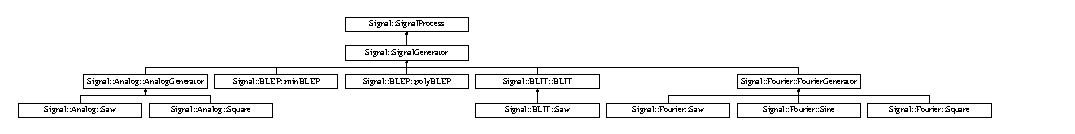
\includegraphics[height=1.346154cm]{classSignal_1_1SignalProcess}
\end{center}
\end{figure}
\subsection*{Public Member Functions}
\begin{DoxyCompactItemize}
\item 
\hyperlink{classSignal_1_1SignalProcess_a3a9b0cdff55c482000faadfcbf57b821}{Signal\+Process} ()
\item 
virtual \hyperlink{classSignal_1_1SignalProcess_aa399b06b43866fd6c1a0e9476f7fe476}{$\sim$\+Signal\+Process} ()
\item 
virtual bool \hyperlink{classSignal_1_1SignalProcess_a7986df989ac8afca3674ae8eace3cfdb}{Perform} (\hyperlink{classSignal_1_1Sample}{Sample} \&signal)=0
\item 
virtual bool \hyperlink{classSignal_1_1SignalProcess_a9584dc515d2167f4439ed3d014bbb3f7}{Perform} (\hyperlink{classSignal_1_1RingBuffer}{Ring\+Buffer} \&signal)=0
\end{DoxyCompactItemize}


\subsection{Detailed Description}


Definition at line 20 of file Signal\+Process.\+h.



\subsection{Constructor \& Destructor Documentation}
\hypertarget{classSignal_1_1SignalProcess_a3a9b0cdff55c482000faadfcbf57b821}{\index{Signal\+::\+Signal\+Process@{Signal\+::\+Signal\+Process}!Signal\+Process@{Signal\+Process}}
\index{Signal\+Process@{Signal\+Process}!Signal\+::\+Signal\+Process@{Signal\+::\+Signal\+Process}}
\subsubsection[{Signal\+Process}]{\setlength{\rightskip}{0pt plus 5cm}Signal\+Process\+::\+Signal\+Process (
\begin{DoxyParamCaption}
{}
\end{DoxyParamCaption}
)}}\label{classSignal_1_1SignalProcess_a3a9b0cdff55c482000faadfcbf57b821}


Definition at line 11 of file Signal\+Process.\+cpp.


\begin{DoxyCode}
11 \{\}
\end{DoxyCode}
\hypertarget{classSignal_1_1SignalProcess_aa399b06b43866fd6c1a0e9476f7fe476}{\index{Signal\+::\+Signal\+Process@{Signal\+::\+Signal\+Process}!````~Signal\+Process@{$\sim$\+Signal\+Process}}
\index{````~Signal\+Process@{$\sim$\+Signal\+Process}!Signal\+::\+Signal\+Process@{Signal\+::\+Signal\+Process}}
\subsubsection[{$\sim$\+Signal\+Process}]{\setlength{\rightskip}{0pt plus 5cm}Signal\+Process\+::$\sim$\+Signal\+Process (
\begin{DoxyParamCaption}
{}
\end{DoxyParamCaption}
)\hspace{0.3cm}{\ttfamily [virtual]}}}\label{classSignal_1_1SignalProcess_aa399b06b43866fd6c1a0e9476f7fe476}


Definition at line 12 of file Signal\+Process.\+cpp.


\begin{DoxyCode}
12 \{\}\end{DoxyCode}


\subsection{Member Function Documentation}
\hypertarget{classSignal_1_1SignalProcess_a7986df989ac8afca3674ae8eace3cfdb}{\index{Signal\+::\+Signal\+Process@{Signal\+::\+Signal\+Process}!Perform@{Perform}}
\index{Perform@{Perform}!Signal\+::\+Signal\+Process@{Signal\+::\+Signal\+Process}}
\subsubsection[{Perform}]{\setlength{\rightskip}{0pt plus 5cm}virtual bool Signal\+::\+Signal\+Process\+::\+Perform (
\begin{DoxyParamCaption}
\item[{{\bf Sample} \&}]{signal}
\end{DoxyParamCaption}
)\hspace{0.3cm}{\ttfamily [inline]}, {\ttfamily [pure virtual]}}}\label{classSignal_1_1SignalProcess_a7986df989ac8afca3674ae8eace3cfdb}


Implemented in \hyperlink{classSignal_1_1Fourier_1_1Sine_aa35c77904f8d7a0de6fa4895d6c53644}{Signal\+::\+Fourier\+::\+Sine}, \hyperlink{classSignal_1_1Fourier_1_1FourierGenerator_a6ec444e7b66d2cb339c001704071646a}{Signal\+::\+Fourier\+::\+Fourier\+Generator}, \hyperlink{classSignal_1_1BLIT_1_1BLIT_a98982b34bc6c9ca4c2e91550afa31375}{Signal\+::\+B\+L\+I\+T\+::\+B\+L\+I\+T}, \hyperlink{classSignal_1_1SignalGenerator_a2cd9061c5ae40a392a9476551b4379f3}{Signal\+::\+Signal\+Generator}, \hyperlink{classSignal_1_1Trivial_1_1TrivialGenerator_a2394cf9d0d40f9d25f72aff03e372ad9}{Signal\+::\+Trivial\+::\+Trivial\+Generator}, \hyperlink{classSignal_1_1Fourier_1_1Saw_adf69eea95516fc9c7d06fae036d2fa9b}{Signal\+::\+Fourier\+::\+Saw}, \hyperlink{classSignal_1_1Fourier_1_1Square_a29e4b9d03b9df4fb6ed0d7a817ecffda}{Signal\+::\+Fourier\+::\+Square}, and \hyperlink{classSignal_1_1Trivial_1_1TrivialSaw_a091e3137a03978cc7dfaecf5b00dad46}{Signal\+::\+Trivial\+::\+Trivial\+Saw}.

\hypertarget{classSignal_1_1SignalProcess_a9584dc515d2167f4439ed3d014bbb3f7}{\index{Signal\+::\+Signal\+Process@{Signal\+::\+Signal\+Process}!Perform@{Perform}}
\index{Perform@{Perform}!Signal\+::\+Signal\+Process@{Signal\+::\+Signal\+Process}}
\subsubsection[{Perform}]{\setlength{\rightskip}{0pt plus 5cm}virtual bool Signal\+::\+Signal\+Process\+::\+Perform (
\begin{DoxyParamCaption}
\item[{{\bf Ring\+Buffer} \&}]{signal}
\end{DoxyParamCaption}
)\hspace{0.3cm}{\ttfamily [inline]}, {\ttfamily [pure virtual]}}}\label{classSignal_1_1SignalProcess_a9584dc515d2167f4439ed3d014bbb3f7}


Implemented in \hyperlink{classSignal_1_1Fourier_1_1Sine_a5d951e5fbfc77354bddab9dfedea008f}{Signal\+::\+Fourier\+::\+Sine}, \hyperlink{classSignal_1_1Fourier_1_1FourierGenerator_acc6a3825eb4060269749a37ae29ee847}{Signal\+::\+Fourier\+::\+Fourier\+Generator}, \hyperlink{classSignal_1_1BLIT_1_1BLIT_a2f0ee604ed0e67557aa9f7e7f50d80ec}{Signal\+::\+B\+L\+I\+T\+::\+B\+L\+I\+T}, \hyperlink{classSignal_1_1SignalGenerator_a126d52dd9b6b14d33efc624e2c89284e}{Signal\+::\+Signal\+Generator}, \hyperlink{classSignal_1_1Trivial_1_1TrivialGenerator_a232aefbb2815eaf25e697ecedeb0f3d9}{Signal\+::\+Trivial\+::\+Trivial\+Generator}, \hyperlink{classSignal_1_1Fourier_1_1Saw_acef099db2217902d7157e5b93f658363}{Signal\+::\+Fourier\+::\+Saw}, \hyperlink{classSignal_1_1Fourier_1_1Square_a7aacafda4427b996b56ad6764ea09177}{Signal\+::\+Fourier\+::\+Square}, and \hyperlink{classSignal_1_1Trivial_1_1TrivialSaw_a22b97c8dfdca76664cbb6e634c85085d}{Signal\+::\+Trivial\+::\+Trivial\+Saw}.



The documentation for this class was generated from the following files\+:\begin{DoxyCompactItemize}
\item 
/\+Users/alexanderzywicki/\+Documents/\+School\+\_\+\+Stuff/\+Fall\+\_\+2014/\+Digital\+\_\+\+Signal\+\_\+\+Generation\+\_\+and\+\_\+\+Analysis/src/include/\hyperlink{SignalProcess_8h}{Signal\+Process.\+h}\item 
/\+Users/alexanderzywicki/\+Documents/\+School\+\_\+\+Stuff/\+Fall\+\_\+2014/\+Digital\+\_\+\+Signal\+\_\+\+Generation\+\_\+and\+\_\+\+Analysis/src/\hyperlink{SignalProcess_8cpp}{Signal\+Process.\+cpp}\end{DoxyCompactItemize}

\hypertarget{classSignal_1_1Sine}{\section{Signal\+:\+:Sine Class Reference}
\label{classSignal_1_1Sine}\index{Signal\+::\+Sine@{Signal\+::\+Sine}}
}


{\ttfamily \#include $<$Sine.\+h$>$}

Inheritance diagram for Signal\+:\+:Sine\+:\begin{figure}[H]
\begin{center}
\leavevmode
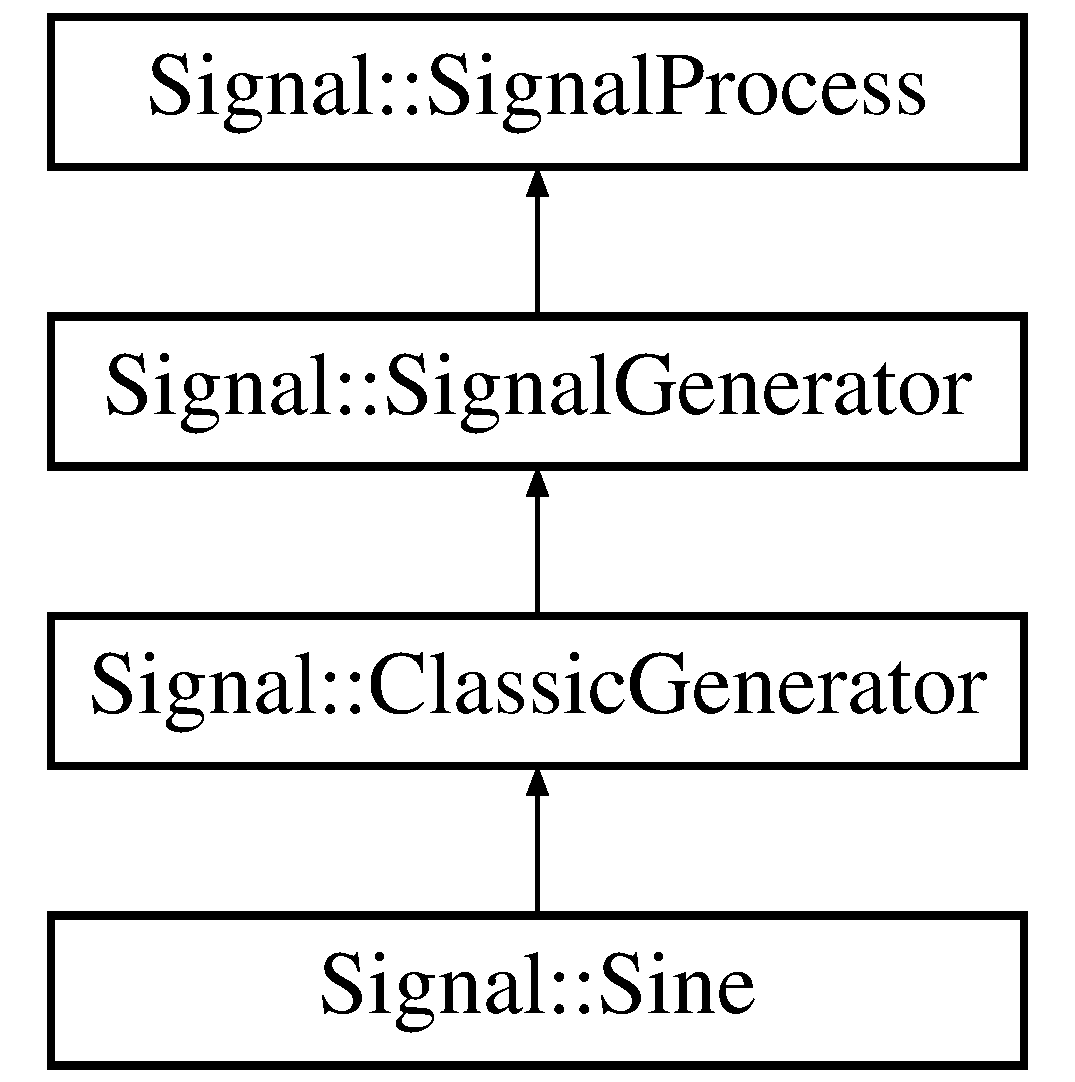
\includegraphics[height=4.000000cm]{classSignal_1_1Sine}
\end{center}
\end{figure}
\subsection*{Public Member Functions}
\begin{DoxyCompactItemize}
\item 
\hyperlink{classSignal_1_1Sine_aa808d1e080ee1c18324eedc020ee0514}{Sine} ()
\item 
\hyperlink{classSignal_1_1Sine_a0dbdf5da8c6baeea56a70f3eb9c3a6fd}{Sine} (double const \&frequency, double const \&phase\+\_\+offset)
\item 
virtual \hyperlink{classSignal_1_1Sine_a0d6a85ad0ddea987aba1955f98be89df}{$\sim$\+Sine} ()
\item 
virtual bool \hyperlink{classSignal_1_1Sine_a8f7c74c35cfd87b490d84a7a75c35691}{Perform} (\hyperlink{classSignal_1_1Sample}{Sample} \&signal)
\item 
virtual bool \hyperlink{classSignal_1_1Sine_ac0a6c6e24f830446ea75de3a392f7e06}{Perform} (\hyperlink{classSignal_1_1RingBuffer}{Ring\+Buffer} \&signal)
\item 
virtual double const \& \hyperlink{classSignal_1_1SignalGenerator_a96af42ee68f94e9b04d034fd68b73ecd}{Frequency} () const 
\item 
virtual double const \& \hyperlink{classSignal_1_1SignalGenerator_af83b532bf3ddc3637c2fd7a1dfd095cb}{Frequency} (double const \&value)
\item 
virtual double const \& \hyperlink{classSignal_1_1SignalGenerator_ac2538ec946f001e394d2416fda698d1c}{Phase\+Offset} () const 
\item 
virtual double const \& \hyperlink{classSignal_1_1SignalGenerator_ac6a103ff72beaa338f6d18c812522d78}{Phase\+Offset} (double const \&value)
\end{DoxyCompactItemize}
\subsection*{Protected Member Functions}
\begin{DoxyCompactItemize}
\item 
unsigned long \hyperlink{classSignal_1_1ClassicGenerator_a7457e912d428de4e3fc27ec7fc49890e}{\+\_\+max\+Harms} (double \+\_\+frq)
\item 
double \hyperlink{classSignal_1_1ClassicGenerator_a255330ce8049b6e6d101b8d356cebe3d}{\+\_\+pstep} ()
\item 
double \hyperlink{classSignal_1_1ClassicGenerator_a6571276f584ff0be3862243d0f103a92}{\+\_\+pstep\+\_\+rad} ()
\item 
void \hyperlink{classSignal_1_1ClassicGenerator_a6454565b655bff7b8335735c2fabb4af}{\+\_\+psync} ()
\end{DoxyCompactItemize}
\subsection*{Protected Attributes}
\begin{DoxyCompactItemize}
\item 
\hyperlink{classSignal_1_1Sample}{Sample} \hyperlink{classSignal_1_1ClassicGenerator_a40313d0d806d6e44af7d41b3ef3a0822}{\+\_\+sample}
\item 
\hyperlink{classSignal_1_1Sample}{Sample} \hyperlink{classSignal_1_1ClassicGenerator_a1214faf589eccb01631700723900bbf9}{\+\_\+storage}
\item 
double \hyperlink{classSignal_1_1ClassicGenerator_ade9b66bc49d2d2f40a1390fc6374b8b2}{\+\_\+phasor}
\item 
double \hyperlink{classSignal_1_1SignalGenerator_a7f107461333bce68c5dad412db96a8c2}{\+\_\+frequency}
\item 
double \hyperlink{classSignal_1_1SignalGenerator_a85a4702347352bab1c71e0a8df8437d6}{\+\_\+f\+Hertz}
\item 
double \hyperlink{classSignal_1_1SignalGenerator_a6b4444d46747c8517171edbbf4b5588f}{\+\_\+phase\+\_\+offset}
\end{DoxyCompactItemize}


\subsection{Detailed Description}


Definition at line 32 of file Sine.\+h.



\subsection{Constructor \& Destructor Documentation}
\hypertarget{classSignal_1_1Sine_aa808d1e080ee1c18324eedc020ee0514}{\index{Signal\+::\+Sine@{Signal\+::\+Sine}!Sine@{Sine}}
\index{Sine@{Sine}!Signal\+::\+Sine@{Signal\+::\+Sine}}
\subsubsection[{Sine}]{\setlength{\rightskip}{0pt plus 5cm}Signal\+::\+Sine\+::\+Sine (
\begin{DoxyParamCaption}
{}
\end{DoxyParamCaption}
)}}\label{classSignal_1_1Sine_aa808d1e080ee1c18324eedc020ee0514}


Definition at line 12 of file Sine.\+cpp.


\begin{DoxyCode}
12 :\hyperlink{classSignal_1_1ClassicGenerator_a7e4478904de77156deccb1515f6985cb}{ClassicGenerator}()\{\}
\end{DoxyCode}
\hypertarget{classSignal_1_1Sine_a0dbdf5da8c6baeea56a70f3eb9c3a6fd}{\index{Signal\+::\+Sine@{Signal\+::\+Sine}!Sine@{Sine}}
\index{Sine@{Sine}!Signal\+::\+Sine@{Signal\+::\+Sine}}
\subsubsection[{Sine}]{\setlength{\rightskip}{0pt plus 5cm}Signal\+::\+Sine\+::\+Sine (
\begin{DoxyParamCaption}
\item[{double const \&}]{frequency, }
\item[{double const \&}]{phase\+\_\+offset}
\end{DoxyParamCaption}
)}}\label{classSignal_1_1Sine_a0dbdf5da8c6baeea56a70f3eb9c3a6fd}


Definition at line 13 of file Sine.\+cpp.


\begin{DoxyCode}
13                                                                   :
      \hyperlink{classSignal_1_1ClassicGenerator_a7e4478904de77156deccb1515f6985cb}{ClassicGenerator}(frequency,phase\_offset)\{
14     \hyperlink{classSignal_1_1ClassicGenerator_a40313d0d806d6e44af7d41b3ef3a0822}{\_sample}=0;
15     \hyperlink{classSignal_1_1ClassicGenerator_a1214faf589eccb01631700723900bbf9}{\_storage}=0;
16 \}
\end{DoxyCode}
\hypertarget{classSignal_1_1Sine_a0d6a85ad0ddea987aba1955f98be89df}{\index{Signal\+::\+Sine@{Signal\+::\+Sine}!````~Sine@{$\sim$\+Sine}}
\index{````~Sine@{$\sim$\+Sine}!Signal\+::\+Sine@{Signal\+::\+Sine}}
\subsubsection[{$\sim$\+Sine}]{\setlength{\rightskip}{0pt plus 5cm}Signal\+::\+Sine\+::$\sim$\+Sine (
\begin{DoxyParamCaption}
{}
\end{DoxyParamCaption}
)\hspace{0.3cm}{\ttfamily [virtual]}}}\label{classSignal_1_1Sine_a0d6a85ad0ddea987aba1955f98be89df}


Definition at line 17 of file Sine.\+cpp.


\begin{DoxyCode}
17 \{\}
\end{DoxyCode}


\subsection{Member Function Documentation}
\hypertarget{classSignal_1_1ClassicGenerator_a7457e912d428de4e3fc27ec7fc49890e}{\index{Signal\+::\+Sine@{Signal\+::\+Sine}!\+\_\+max\+Harms@{\+\_\+max\+Harms}}
\index{\+\_\+max\+Harms@{\+\_\+max\+Harms}!Signal\+::\+Sine@{Signal\+::\+Sine}}
\subsubsection[{\+\_\+max\+Harms}]{\setlength{\rightskip}{0pt plus 5cm}unsigned long Signal\+::\+Classic\+Generator\+::\+\_\+max\+Harms (
\begin{DoxyParamCaption}
\item[{double}]{\+\_\+frq}
\end{DoxyParamCaption}
)\hspace{0.3cm}{\ttfamily [inline]}, {\ttfamily [protected]}, {\ttfamily [inherited]}}}\label{classSignal_1_1ClassicGenerator_a7457e912d428de4e3fc27ec7fc49890e}


Definition at line 70 of file Classic\+Generator.\+h.


\begin{DoxyCode}
70                                                                \{
71         \textcolor{comment}{//double softLim = 0.45;}
72         \textcolor{comment}{//double hardLim = 0.5;}
73         \textcolor{keywordtype}{double} \_s = \hyperlink{namespaceSignal_ae7b1f222afc010e0f33f306f978fcde9}{Sample\_Rate}()* 0.45;
74         \_s/=\_frq;
75         \textcolor{keywordflow}{return} trunc(\_s);
76     \}
\end{DoxyCode}
\hypertarget{classSignal_1_1ClassicGenerator_a255330ce8049b6e6d101b8d356cebe3d}{\index{Signal\+::\+Sine@{Signal\+::\+Sine}!\+\_\+pstep@{\+\_\+pstep}}
\index{\+\_\+pstep@{\+\_\+pstep}!Signal\+::\+Sine@{Signal\+::\+Sine}}
\subsubsection[{\+\_\+pstep}]{\setlength{\rightskip}{0pt plus 5cm}double Signal\+::\+Classic\+Generator\+::\+\_\+pstep (
\begin{DoxyParamCaption}
{}
\end{DoxyParamCaption}
)\hspace{0.3cm}{\ttfamily [inline]}, {\ttfamily [protected]}, {\ttfamily [inherited]}}}\label{classSignal_1_1ClassicGenerator_a255330ce8049b6e6d101b8d356cebe3d}


Definition at line 57 of file Classic\+Generator.\+h.


\begin{DoxyCode}
57                                           \{
58         \textcolor{keywordtype}{double} value = \hyperlink{classSignal_1_1ClassicGenerator_ade9b66bc49d2d2f40a1390fc6374b8b2}{\_phasor};
59         \hyperlink{classSignal_1_1ClassicGenerator_ade9b66bc49d2d2f40a1390fc6374b8b2}{\_phasor}+=\hyperlink{classSignal_1_1SignalGenerator_a7f107461333bce68c5dad412db96a8c2}{\_frequency};
60         \hyperlink{classSignal_1_1ClassicGenerator_ade9b66bc49d2d2f40a1390fc6374b8b2}{\_phasor} = \hyperlink{classSignal_1_1ClassicGenerator_ade9b66bc49d2d2f40a1390fc6374b8b2}{\_phasor}-(\textcolor{keywordtype}{unsigned} long)\hyperlink{classSignal_1_1ClassicGenerator_ade9b66bc49d2d2f40a1390fc6374b8b2}{\_phasor};\textcolor{comment}{//cheaper %1}
61         \textcolor{keywordflow}{return} value;
62     \}
\end{DoxyCode}
\hypertarget{classSignal_1_1ClassicGenerator_a6571276f584ff0be3862243d0f103a92}{\index{Signal\+::\+Sine@{Signal\+::\+Sine}!\+\_\+pstep\+\_\+rad@{\+\_\+pstep\+\_\+rad}}
\index{\+\_\+pstep\+\_\+rad@{\+\_\+pstep\+\_\+rad}!Signal\+::\+Sine@{Signal\+::\+Sine}}
\subsubsection[{\+\_\+pstep\+\_\+rad}]{\setlength{\rightskip}{0pt plus 5cm}double Signal\+::\+Classic\+Generator\+::\+\_\+pstep\+\_\+rad (
\begin{DoxyParamCaption}
{}
\end{DoxyParamCaption}
)\hspace{0.3cm}{\ttfamily [inline]}, {\ttfamily [protected]}, {\ttfamily [inherited]}}}\label{classSignal_1_1ClassicGenerator_a6571276f584ff0be3862243d0f103a92}


Definition at line 63 of file Classic\+Generator.\+h.


\begin{DoxyCode}
63                                               \{
64         \textcolor{keywordflow}{return} \hyperlink{PI_8h_a4912c64aec0c943b7985db6cb61ff83a}{TWOPI} * \hyperlink{classSignal_1_1ClassicGenerator_a255330ce8049b6e6d101b8d356cebe3d}{\_pstep}();
65     \}
\end{DoxyCode}
\hypertarget{classSignal_1_1ClassicGenerator_a6454565b655bff7b8335735c2fabb4af}{\index{Signal\+::\+Sine@{Signal\+::\+Sine}!\+\_\+psync@{\+\_\+psync}}
\index{\+\_\+psync@{\+\_\+psync}!Signal\+::\+Sine@{Signal\+::\+Sine}}
\subsubsection[{\+\_\+psync}]{\setlength{\rightskip}{0pt plus 5cm}void Signal\+::\+Classic\+Generator\+::\+\_\+psync (
\begin{DoxyParamCaption}
{}
\end{DoxyParamCaption}
)\hspace{0.3cm}{\ttfamily [inline]}, {\ttfamily [protected]}, {\ttfamily [inherited]}}}\label{classSignal_1_1ClassicGenerator_a6454565b655bff7b8335735c2fabb4af}


Definition at line 66 of file Classic\+Generator.\+h.


\begin{DoxyCode}
66                                         \{
67         \hyperlink{classSignal_1_1ClassicGenerator_ade9b66bc49d2d2f40a1390fc6374b8b2}{\_phasor} = 0;
68     \}
\end{DoxyCode}
\hypertarget{classSignal_1_1SignalGenerator_a96af42ee68f94e9b04d034fd68b73ecd}{\index{Signal\+::\+Sine@{Signal\+::\+Sine}!Frequency@{Frequency}}
\index{Frequency@{Frequency}!Signal\+::\+Sine@{Signal\+::\+Sine}}
\subsubsection[{Frequency}]{\setlength{\rightskip}{0pt plus 5cm}double const \& Signal\+::\+Signal\+Generator\+::\+Frequency (
\begin{DoxyParamCaption}
{}
\end{DoxyParamCaption}
) const\hspace{0.3cm}{\ttfamily [virtual]}, {\ttfamily [inherited]}}}\label{classSignal_1_1SignalGenerator_a96af42ee68f94e9b04d034fd68b73ecd}


Definition at line 16 of file Signal\+Generator.\+cpp.


\begin{DoxyCode}
16                                                    \{
17     \textcolor{keywordflow}{return} \hyperlink{classSignal_1_1SignalGenerator_a85a4702347352bab1c71e0a8df8437d6}{\_fHertz};
18 \}
\end{DoxyCode}
\hypertarget{classSignal_1_1SignalGenerator_af83b532bf3ddc3637c2fd7a1dfd095cb}{\index{Signal\+::\+Sine@{Signal\+::\+Sine}!Frequency@{Frequency}}
\index{Frequency@{Frequency}!Signal\+::\+Sine@{Signal\+::\+Sine}}
\subsubsection[{Frequency}]{\setlength{\rightskip}{0pt plus 5cm}double const \& Signal\+::\+Signal\+Generator\+::\+Frequency (
\begin{DoxyParamCaption}
\item[{double const \&}]{value}
\end{DoxyParamCaption}
)\hspace{0.3cm}{\ttfamily [virtual]}, {\ttfamily [inherited]}}}\label{classSignal_1_1SignalGenerator_af83b532bf3ddc3637c2fd7a1dfd095cb}


Reimplemented in \hyperlink{classSignal_1_1BLIT_1_1BLIT_a59110620478308054d4c932c613e5cc6}{Signal\+::\+B\+L\+I\+T\+::\+B\+L\+I\+T}, \hyperlink{classSignal_1_1Saw_af91fd0d15b380c02e309705eaad46efd}{Signal\+::\+Saw}, and \hyperlink{classSignal_1_1Square_a19f966d5b1800f5487cdd164747b21c0}{Signal\+::\+Square}.



Definition at line 19 of file Signal\+Generator.\+cpp.


\begin{DoxyCode}
19                                                                  \{
20     \hyperlink{classSignal_1_1SignalGenerator_a85a4702347352bab1c71e0a8df8437d6}{\_fHertz} = value;
21     \hyperlink{classSignal_1_1SignalGenerator_a7f107461333bce68c5dad412db96a8c2}{\_frequency} = \hyperlink{classSignal_1_1SignalGenerator_a85a4702347352bab1c71e0a8df8437d6}{\_fHertz}/\hyperlink{namespaceSignal_ae7b1f222afc010e0f33f306f978fcde9}{Sample\_Rate}();
22     \textcolor{keywordflow}{return} \hyperlink{classSignal_1_1SignalGenerator_a85a4702347352bab1c71e0a8df8437d6}{\_fHertz};
23 \}
\end{DoxyCode}
\hypertarget{classSignal_1_1Sine_a8f7c74c35cfd87b490d84a7a75c35691}{\index{Signal\+::\+Sine@{Signal\+::\+Sine}!Perform@{Perform}}
\index{Perform@{Perform}!Signal\+::\+Sine@{Signal\+::\+Sine}}
\subsubsection[{Perform}]{\setlength{\rightskip}{0pt plus 5cm}bool Signal\+::\+Sine\+::\+Perform (
\begin{DoxyParamCaption}
\item[{{\bf Sample} \&}]{signal}
\end{DoxyParamCaption}
)\hspace{0.3cm}{\ttfamily [inline]}, {\ttfamily [virtual]}}}\label{classSignal_1_1Sine_a8f7c74c35cfd87b490d84a7a75c35691}


Reimplemented from \hyperlink{classSignal_1_1ClassicGenerator_a4a62f329b9cd64d92b07f53c4d593356}{Signal\+::\+Classic\+Generator}.



Definition at line 41 of file Sine.\+h.


\begin{DoxyCode}
41                                            \{
42         \textcolor{comment}{//uses LUT}
43 \textcolor{preprocessor}{#if SINE\_IMPL == SINE\_USE\_LUT}
44         signal = \hyperlink{namespaceSignal_a1ae06d442767e736f514051fcc61d254}{sine}((\hyperlink{classSignal_1_1ClassicGenerator_a255330ce8049b6e6d101b8d356cebe3d}{\_pstep}() + \hyperlink{classSignal_1_1SignalGenerator_a6b4444d46747c8517171edbbf4b5588f}{\_phase\_offset}));
45 \textcolor{preprocessor}{#elif SINE\_IMPL==SINE\_USE\_TAYLOR}
46         signal = \hyperlink{namespaceBackend_1_1Taylor_afda165e6dde636dd0f7b32031a71c7df}{Backend::Taylor::Sine}((\hyperlink{classSignal_1_1ClassicGenerator_a255330ce8049b6e6d101b8d356cebe3d}{\_pstep}()+
      \hyperlink{classSignal_1_1SignalGenerator_a6b4444d46747c8517171edbbf4b5588f}{\_phase\_offset})*\hyperlink{PI_8h_a4912c64aec0c943b7985db6cb61ff83a}{TWOPI});
47 \textcolor{preprocessor}{#else}
48         signal = sin((\hyperlink{classSignal_1_1ClassicGenerator_a255330ce8049b6e6d101b8d356cebe3d}{\_pstep}()+\hyperlink{classSignal_1_1SignalGenerator_a6b4444d46747c8517171edbbf4b5588f}{\_phase\_offset})*\hyperlink{PI_8h_a4912c64aec0c943b7985db6cb61ff83a}{TWOPI});
49 \textcolor{preprocessor}{#endif}
50 
51         \textcolor{keywordflow}{return} \textcolor{keyword}{true};
52     \}
\end{DoxyCode}
\hypertarget{classSignal_1_1Sine_ac0a6c6e24f830446ea75de3a392f7e06}{\index{Signal\+::\+Sine@{Signal\+::\+Sine}!Perform@{Perform}}
\index{Perform@{Perform}!Signal\+::\+Sine@{Signal\+::\+Sine}}
\subsubsection[{Perform}]{\setlength{\rightskip}{0pt plus 5cm}bool Signal\+::\+Sine\+::\+Perform (
\begin{DoxyParamCaption}
\item[{{\bf Ring\+Buffer} \&}]{signal}
\end{DoxyParamCaption}
)\hspace{0.3cm}{\ttfamily [inline]}, {\ttfamily [virtual]}}}\label{classSignal_1_1Sine_ac0a6c6e24f830446ea75de3a392f7e06}


Reimplemented from \hyperlink{classSignal_1_1ClassicGenerator_a308c13baa66020d44c2227bd58db4b4f}{Signal\+::\+Classic\+Generator}.



Definition at line 53 of file Sine.\+h.


\begin{DoxyCode}
53                                                \{
54         signal.Flush();
55         \textcolor{keywordflow}{while} (!signal.Full()) \{
56             \textcolor{keywordflow}{if} (\hyperlink{classSignal_1_1Sine_a8f7c74c35cfd87b490d84a7a75c35691}{Perform}(\hyperlink{classSignal_1_1ClassicGenerator_a40313d0d806d6e44af7d41b3ef3a0822}{\_sample})) \{
57                 \textcolor{keywordflow}{if}(signal.Write(\hyperlink{classSignal_1_1ClassicGenerator_a40313d0d806d6e44af7d41b3ef3a0822}{\_sample}))\{
58                 \}\textcolor{keywordflow}{else} \textcolor{keywordflow}{return} \textcolor{keyword}{false};
59             \}\textcolor{keywordflow}{else} \textcolor{keywordflow}{return} \textcolor{keyword}{false};
60         \}\textcolor{keywordflow}{return} \textcolor{keyword}{true};
61     \}
\end{DoxyCode}
\hypertarget{classSignal_1_1SignalGenerator_ac2538ec946f001e394d2416fda698d1c}{\index{Signal\+::\+Sine@{Signal\+::\+Sine}!Phase\+Offset@{Phase\+Offset}}
\index{Phase\+Offset@{Phase\+Offset}!Signal\+::\+Sine@{Signal\+::\+Sine}}
\subsubsection[{Phase\+Offset}]{\setlength{\rightskip}{0pt plus 5cm}double const \& Signal\+::\+Signal\+Generator\+::\+Phase\+Offset (
\begin{DoxyParamCaption}
{}
\end{DoxyParamCaption}
) const\hspace{0.3cm}{\ttfamily [virtual]}, {\ttfamily [inherited]}}}\label{classSignal_1_1SignalGenerator_ac2538ec946f001e394d2416fda698d1c}


Definition at line 24 of file Signal\+Generator.\+cpp.


\begin{DoxyCode}
24                                                      \{
25     \textcolor{keywordflow}{return} \hyperlink{classSignal_1_1SignalGenerator_a6b4444d46747c8517171edbbf4b5588f}{\_phase\_offset};
26 \}
\end{DoxyCode}
\hypertarget{classSignal_1_1SignalGenerator_ac6a103ff72beaa338f6d18c812522d78}{\index{Signal\+::\+Sine@{Signal\+::\+Sine}!Phase\+Offset@{Phase\+Offset}}
\index{Phase\+Offset@{Phase\+Offset}!Signal\+::\+Sine@{Signal\+::\+Sine}}
\subsubsection[{Phase\+Offset}]{\setlength{\rightskip}{0pt plus 5cm}double const \& Signal\+::\+Signal\+Generator\+::\+Phase\+Offset (
\begin{DoxyParamCaption}
\item[{double const \&}]{value}
\end{DoxyParamCaption}
)\hspace{0.3cm}{\ttfamily [virtual]}, {\ttfamily [inherited]}}}\label{classSignal_1_1SignalGenerator_ac6a103ff72beaa338f6d18c812522d78}


Definition at line 27 of file Signal\+Generator.\+cpp.


\begin{DoxyCode}
27                                                                    \{
28     \hyperlink{classSignal_1_1SignalGenerator_a6b4444d46747c8517171edbbf4b5588f}{\_phase\_offset} = value;
29     \textcolor{keywordflow}{return} \hyperlink{classSignal_1_1SignalGenerator_a6b4444d46747c8517171edbbf4b5588f}{\_phase\_offset};
30 \}
\end{DoxyCode}


\subsection{Member Data Documentation}
\hypertarget{classSignal_1_1SignalGenerator_a85a4702347352bab1c71e0a8df8437d6}{\index{Signal\+::\+Sine@{Signal\+::\+Sine}!\+\_\+f\+Hertz@{\+\_\+f\+Hertz}}
\index{\+\_\+f\+Hertz@{\+\_\+f\+Hertz}!Signal\+::\+Sine@{Signal\+::\+Sine}}
\subsubsection[{\+\_\+f\+Hertz}]{\setlength{\rightskip}{0pt plus 5cm}double Signal\+::\+Signal\+Generator\+::\+\_\+f\+Hertz\hspace{0.3cm}{\ttfamily [protected]}, {\ttfamily [inherited]}}}\label{classSignal_1_1SignalGenerator_a85a4702347352bab1c71e0a8df8437d6}


Definition at line 34 of file Signal\+Generator.\+h.

\hypertarget{classSignal_1_1SignalGenerator_a7f107461333bce68c5dad412db96a8c2}{\index{Signal\+::\+Sine@{Signal\+::\+Sine}!\+\_\+frequency@{\+\_\+frequency}}
\index{\+\_\+frequency@{\+\_\+frequency}!Signal\+::\+Sine@{Signal\+::\+Sine}}
\subsubsection[{\+\_\+frequency}]{\setlength{\rightskip}{0pt plus 5cm}double Signal\+::\+Signal\+Generator\+::\+\_\+frequency\hspace{0.3cm}{\ttfamily [protected]}, {\ttfamily [inherited]}}}\label{classSignal_1_1SignalGenerator_a7f107461333bce68c5dad412db96a8c2}


Definition at line 33 of file Signal\+Generator.\+h.

\hypertarget{classSignal_1_1SignalGenerator_a6b4444d46747c8517171edbbf4b5588f}{\index{Signal\+::\+Sine@{Signal\+::\+Sine}!\+\_\+phase\+\_\+offset@{\+\_\+phase\+\_\+offset}}
\index{\+\_\+phase\+\_\+offset@{\+\_\+phase\+\_\+offset}!Signal\+::\+Sine@{Signal\+::\+Sine}}
\subsubsection[{\+\_\+phase\+\_\+offset}]{\setlength{\rightskip}{0pt plus 5cm}double Signal\+::\+Signal\+Generator\+::\+\_\+phase\+\_\+offset\hspace{0.3cm}{\ttfamily [protected]}, {\ttfamily [inherited]}}}\label{classSignal_1_1SignalGenerator_a6b4444d46747c8517171edbbf4b5588f}


Definition at line 35 of file Signal\+Generator.\+h.

\hypertarget{classSignal_1_1ClassicGenerator_ade9b66bc49d2d2f40a1390fc6374b8b2}{\index{Signal\+::\+Sine@{Signal\+::\+Sine}!\+\_\+phasor@{\+\_\+phasor}}
\index{\+\_\+phasor@{\+\_\+phasor}!Signal\+::\+Sine@{Signal\+::\+Sine}}
\subsubsection[{\+\_\+phasor}]{\setlength{\rightskip}{0pt plus 5cm}double Signal\+::\+Classic\+Generator\+::\+\_\+phasor\hspace{0.3cm}{\ttfamily [protected]}, {\ttfamily [inherited]}}}\label{classSignal_1_1ClassicGenerator_ade9b66bc49d2d2f40a1390fc6374b8b2}


Definition at line 41 of file Classic\+Generator.\+h.

\hypertarget{classSignal_1_1ClassicGenerator_a40313d0d806d6e44af7d41b3ef3a0822}{\index{Signal\+::\+Sine@{Signal\+::\+Sine}!\+\_\+sample@{\+\_\+sample}}
\index{\+\_\+sample@{\+\_\+sample}!Signal\+::\+Sine@{Signal\+::\+Sine}}
\subsubsection[{\+\_\+sample}]{\setlength{\rightskip}{0pt plus 5cm}{\bf Sample} Signal\+::\+Classic\+Generator\+::\+\_\+sample\hspace{0.3cm}{\ttfamily [protected]}, {\ttfamily [inherited]}}}\label{classSignal_1_1ClassicGenerator_a40313d0d806d6e44af7d41b3ef3a0822}


Definition at line 34 of file Classic\+Generator.\+h.

\hypertarget{classSignal_1_1ClassicGenerator_a1214faf589eccb01631700723900bbf9}{\index{Signal\+::\+Sine@{Signal\+::\+Sine}!\+\_\+storage@{\+\_\+storage}}
\index{\+\_\+storage@{\+\_\+storage}!Signal\+::\+Sine@{Signal\+::\+Sine}}
\subsubsection[{\+\_\+storage}]{\setlength{\rightskip}{0pt plus 5cm}{\bf Sample} Signal\+::\+Classic\+Generator\+::\+\_\+storage\hspace{0.3cm}{\ttfamily [protected]}, {\ttfamily [inherited]}}}\label{classSignal_1_1ClassicGenerator_a1214faf589eccb01631700723900bbf9}


Definition at line 35 of file Classic\+Generator.\+h.



The documentation for this class was generated from the following files\+:\begin{DoxyCompactItemize}
\item 
/\+Users/alexanderzywicki/\+Documents/\+School\+\_\+\+Stuff/\+Fall\+\_\+2014/\+Digital\+\_\+\+Signal\+\_\+\+Generation\+\_\+and\+\_\+\+Analysis/src/include/\hyperlink{Sine_8h}{Sine.\+h}\item 
/\+Users/alexanderzywicki/\+Documents/\+School\+\_\+\+Stuff/\+Fall\+\_\+2014/\+Digital\+\_\+\+Signal\+\_\+\+Generation\+\_\+and\+\_\+\+Analysis/src/\hyperlink{Sine_8cpp}{Sine.\+cpp}\end{DoxyCompactItemize}

\hypertarget{classBackend_1_1SineLUT}{\section{Backend\+:\+:Sine\+L\+U\+T$<$ element, size $>$ Class Template Reference}
\label{classBackend_1_1SineLUT}\index{Backend\+::\+Sine\+L\+U\+T$<$ element, size $>$@{Backend\+::\+Sine\+L\+U\+T$<$ element, size $>$}}
}


{\ttfamily \#include $<$Sine\+L\+U\+T.\+h$>$}

Inheritance diagram for Backend\+:\+:Sine\+L\+U\+T$<$ element, size $>$\+:\begin{figure}[H]
\begin{center}
\leavevmode
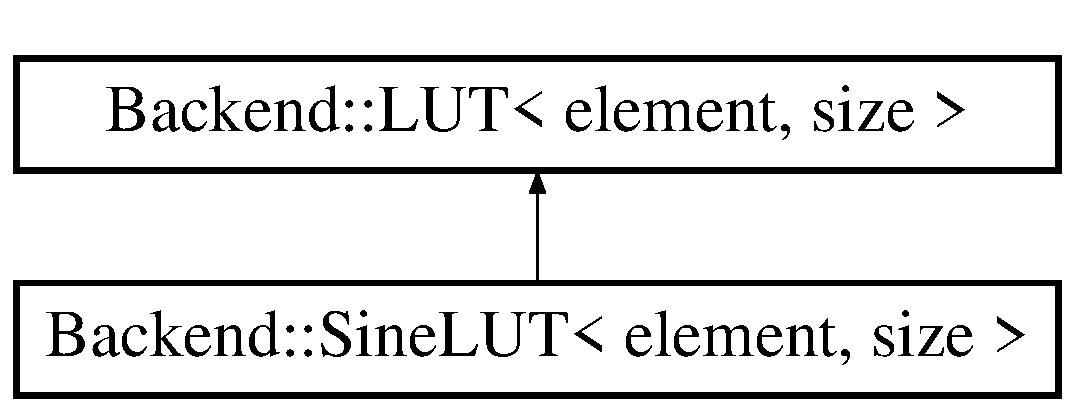
\includegraphics[height=2.000000cm]{classBackend_1_1SineLUT}
\end{center}
\end{figure}
\subsection*{Public Member Functions}
\begin{DoxyCompactItemize}
\item 
\hyperlink{classBackend_1_1SineLUT_ab2784ed19d66ee885ffe23f3ef9d2214}{Sine\+L\+U\+T} ()
\item 
virtual \hyperlink{classBackend_1_1SineLUT_aeb5493bee1755391cea3690c31b1665b}{$\sim$\+Sine\+L\+U\+T} ()
\item 
virtual element \hyperlink{classBackend_1_1SineLUT_a461395dab282ae8ac9b517caf2d6a553}{operator()} (double const \&x)
\item 
element const \& \hyperlink{classBackend_1_1LUT_a9a7c75f36c72778098a091db3269c29c}{operator\mbox{[}$\,$\mbox{]}} (unsigned long const \&index)
\item 
unsigned long const \& \hyperlink{classBackend_1_1LUT_a3ab84f04569e89cd6046da599c6edbae}{Size} () const 
\end{DoxyCompactItemize}
\subsection*{Protected Attributes}
\begin{DoxyCompactItemize}
\item 
double \hyperlink{classBackend_1_1SineLUT_af5d1e8bc8bda7d41272c17e0f2e9aad8}{phs}
\item 
element \hyperlink{classBackend_1_1LUT_ae70f3f0c9aaa9e0b85517d8e2c61d9a5}{\+\_\+table} \mbox{[}size\mbox{]}
\item 
const unsigned long \hyperlink{classBackend_1_1LUT_a94d2ce1a7c644ce2d4f8e905790b9b54}{\+\_\+size}
\end{DoxyCompactItemize}


\subsection{Detailed Description}
\subsubsection*{template$<$typename element, unsigned long size$>$class Backend\+::\+Sine\+L\+U\+T$<$ element, size $>$}



Definition at line 21 of file Sine\+L\+U\+T.\+h.



\subsection{Constructor \& Destructor Documentation}
\hypertarget{classBackend_1_1SineLUT_ab2784ed19d66ee885ffe23f3ef9d2214}{\index{Backend\+::\+Sine\+L\+U\+T@{Backend\+::\+Sine\+L\+U\+T}!Sine\+L\+U\+T@{Sine\+L\+U\+T}}
\index{Sine\+L\+U\+T@{Sine\+L\+U\+T}!Backend\+::\+Sine\+L\+U\+T@{Backend\+::\+Sine\+L\+U\+T}}
\subsubsection[{Sine\+L\+U\+T}]{\setlength{\rightskip}{0pt plus 5cm}template$<$typename element, unsigned long size$>$ {\bf Backend\+::\+Sine\+L\+U\+T}$<$ element, size $>$\+::{\bf Sine\+L\+U\+T} (
\begin{DoxyParamCaption}
{}
\end{DoxyParamCaption}
)\hspace{0.3cm}{\ttfamily [inline]}}}\label{classBackend_1_1SineLUT_ab2784ed19d66ee885ffe23f3ef9d2214}


Definition at line 23 of file Sine\+L\+U\+T.\+h.


\begin{DoxyCode}
23                  :LUT<element,size>()\{
24             \textcolor{keywordtype}{double} step = (\hyperlink{PI_8h_a4912c64aec0c943b7985db6cb61ff83a}{TWOPI}/this->\hyperlink{classBackend_1_1LUT_a94d2ce1a7c644ce2d4f8e905790b9b54}{\_size});
25             \textcolor{keywordtype}{double} \hyperlink{classBackend_1_1SineLUT_af5d1e8bc8bda7d41272c17e0f2e9aad8}{phs}=0;
26             \textcolor{keywordflow}{for} (\textcolor{keywordtype}{int} i=0; i<this->\hyperlink{classBackend_1_1LUT_a94d2ce1a7c644ce2d4f8e905790b9b54}{\_size}; ++i) \{
27                 this->\hyperlink{classBackend_1_1LUT_ae70f3f0c9aaa9e0b85517d8e2c61d9a5}{\_table}[i] = sin(phs);
28                 phs+=step;
29             \}
30         \}
\end{DoxyCode}
\hypertarget{classBackend_1_1SineLUT_aeb5493bee1755391cea3690c31b1665b}{\index{Backend\+::\+Sine\+L\+U\+T@{Backend\+::\+Sine\+L\+U\+T}!````~Sine\+L\+U\+T@{$\sim$\+Sine\+L\+U\+T}}
\index{````~Sine\+L\+U\+T@{$\sim$\+Sine\+L\+U\+T}!Backend\+::\+Sine\+L\+U\+T@{Backend\+::\+Sine\+L\+U\+T}}
\subsubsection[{$\sim$\+Sine\+L\+U\+T}]{\setlength{\rightskip}{0pt plus 5cm}template$<$typename element, unsigned long size$>$ virtual {\bf Backend\+::\+Sine\+L\+U\+T}$<$ element, size $>$\+::$\sim${\bf Sine\+L\+U\+T} (
\begin{DoxyParamCaption}
{}
\end{DoxyParamCaption}
)\hspace{0.3cm}{\ttfamily [inline]}, {\ttfamily [virtual]}}}\label{classBackend_1_1SineLUT_aeb5493bee1755391cea3690c31b1665b}


Definition at line 31 of file Sine\+L\+U\+T.\+h.


\begin{DoxyCode}
31 \{\}
\end{DoxyCode}


\subsection{Member Function Documentation}
\hypertarget{classBackend_1_1SineLUT_a461395dab282ae8ac9b517caf2d6a553}{\index{Backend\+::\+Sine\+L\+U\+T@{Backend\+::\+Sine\+L\+U\+T}!operator()@{operator()}}
\index{operator()@{operator()}!Backend\+::\+Sine\+L\+U\+T@{Backend\+::\+Sine\+L\+U\+T}}
\subsubsection[{operator()}]{\setlength{\rightskip}{0pt plus 5cm}template$<$typename element, unsigned long size$>$ virtual element {\bf Backend\+::\+Sine\+L\+U\+T}$<$ element, size $>$\+::operator() (
\begin{DoxyParamCaption}
\item[{double const \&}]{x}
\end{DoxyParamCaption}
)\hspace{0.3cm}{\ttfamily [inline]}, {\ttfamily [virtual]}}}\label{classBackend_1_1SineLUT_a461395dab282ae8ac9b517caf2d6a553}


Reimplemented from \hyperlink{classBackend_1_1LUT_aea3420a7a3552f38ba8f9ea979bab764}{Backend\+::\+L\+U\+T$<$ element, size $>$}.



Definition at line 32 of file Sine\+L\+U\+T.\+h.


\begin{DoxyCode}
32                                                           \{
33             \hyperlink{classBackend_1_1SineLUT_af5d1e8bc8bda7d41272c17e0f2e9aad8}{phs}=x;
34             \textcolor{comment}{//need range checking on x to ensure 0-1 range}
35             \hyperlink{classBackend_1_1SineLUT_af5d1e8bc8bda7d41272c17e0f2e9aad8}{phs}=fabs(\hyperlink{classBackend_1_1SineLUT_af5d1e8bc8bda7d41272c17e0f2e9aad8}{phs});
36             \hyperlink{classBackend_1_1SineLUT_af5d1e8bc8bda7d41272c17e0f2e9aad8}{phs}=\hyperlink{classBackend_1_1SineLUT_af5d1e8bc8bda7d41272c17e0f2e9aad8}{phs}-((int)\hyperlink{classBackend_1_1SineLUT_af5d1e8bc8bda7d41272c17e0f2e9aad8}{phs});
37             \textcolor{keywordflow}{return} this->\hyperlink{classBackend_1_1LUT_ae70f3f0c9aaa9e0b85517d8e2c61d9a5}{\_table}[(unsigned)(\hyperlink{classBackend_1_1SineLUT_af5d1e8bc8bda7d41272c17e0f2e9aad8}{phs}* (this->\hyperlink{classBackend_1_1LUT_a94d2ce1a7c644ce2d4f8e905790b9b54}{\_size}-1))];
38             
39             \textcolor{keywordflow}{return} 0;
40         \}
\end{DoxyCode}
\hypertarget{classBackend_1_1LUT_a9a7c75f36c72778098a091db3269c29c}{\index{Backend\+::\+Sine\+L\+U\+T@{Backend\+::\+Sine\+L\+U\+T}!operator\mbox{[}$\,$\mbox{]}@{operator[]}}
\index{operator\mbox{[}$\,$\mbox{]}@{operator[]}!Backend\+::\+Sine\+L\+U\+T@{Backend\+::\+Sine\+L\+U\+T}}
\subsubsection[{operator[]}]{\setlength{\rightskip}{0pt plus 5cm}template$<$typename element, unsigned long size$>$ element const\& {\bf Backend\+::\+L\+U\+T}$<$ element, size $>$\+::operator\mbox{[}$\,$\mbox{]} (
\begin{DoxyParamCaption}
\item[{unsigned long const \&}]{index}
\end{DoxyParamCaption}
)\hspace{0.3cm}{\ttfamily [inline]}, {\ttfamily [inherited]}}}\label{classBackend_1_1LUT_a9a7c75f36c72778098a091db3269c29c}


Definition at line 22 of file L\+U\+T.\+h.


\begin{DoxyCode}
22                                                              \{
23 \textcolor{preprocessor}{#ifdef DEBUG}
24             assert(index<\hyperlink{classBackend_1_1LUT_a94d2ce1a7c644ce2d4f8e905790b9b54}{\_size});
25 \textcolor{preprocessor}{#endif}
26             \textcolor{keywordflow}{return} \hyperlink{classBackend_1_1LUT_ae70f3f0c9aaa9e0b85517d8e2c61d9a5}{\_table}[index];
27         \}
\end{DoxyCode}
\hypertarget{classBackend_1_1LUT_a3ab84f04569e89cd6046da599c6edbae}{\index{Backend\+::\+Sine\+L\+U\+T@{Backend\+::\+Sine\+L\+U\+T}!Size@{Size}}
\index{Size@{Size}!Backend\+::\+Sine\+L\+U\+T@{Backend\+::\+Sine\+L\+U\+T}}
\subsubsection[{Size}]{\setlength{\rightskip}{0pt plus 5cm}template$<$typename element, unsigned long size$>$ unsigned long const\& {\bf Backend\+::\+L\+U\+T}$<$ element, size $>$\+::Size (
\begin{DoxyParamCaption}
{}
\end{DoxyParamCaption}
) const\hspace{0.3cm}{\ttfamily [inline]}, {\ttfamily [inherited]}}}\label{classBackend_1_1LUT_a3ab84f04569e89cd6046da599c6edbae}


Definition at line 31 of file L\+U\+T.\+h.


\begin{DoxyCode}
31                                         \{
32             \textcolor{keywordflow}{return} \hyperlink{classBackend_1_1LUT_a94d2ce1a7c644ce2d4f8e905790b9b54}{\_size};
33         \}
\end{DoxyCode}


\subsection{Member Data Documentation}
\hypertarget{classBackend_1_1LUT_a94d2ce1a7c644ce2d4f8e905790b9b54}{\index{Backend\+::\+Sine\+L\+U\+T@{Backend\+::\+Sine\+L\+U\+T}!\+\_\+size@{\+\_\+size}}
\index{\+\_\+size@{\+\_\+size}!Backend\+::\+Sine\+L\+U\+T@{Backend\+::\+Sine\+L\+U\+T}}
\subsubsection[{\+\_\+size}]{\setlength{\rightskip}{0pt plus 5cm}template$<$typename element, unsigned long size$>$ const unsigned long {\bf Backend\+::\+L\+U\+T}$<$ element, size $>$\+::\+\_\+size\hspace{0.3cm}{\ttfamily [protected]}, {\ttfamily [inherited]}}}\label{classBackend_1_1LUT_a94d2ce1a7c644ce2d4f8e905790b9b54}


Definition at line 36 of file L\+U\+T.\+h.

\hypertarget{classBackend_1_1LUT_ae70f3f0c9aaa9e0b85517d8e2c61d9a5}{\index{Backend\+::\+Sine\+L\+U\+T@{Backend\+::\+Sine\+L\+U\+T}!\+\_\+table@{\+\_\+table}}
\index{\+\_\+table@{\+\_\+table}!Backend\+::\+Sine\+L\+U\+T@{Backend\+::\+Sine\+L\+U\+T}}
\subsubsection[{\+\_\+table}]{\setlength{\rightskip}{0pt plus 5cm}template$<$typename element, unsigned long size$>$ element {\bf Backend\+::\+L\+U\+T}$<$ element, size $>$\+::\+\_\+table\mbox{[}size\mbox{]}\hspace{0.3cm}{\ttfamily [protected]}, {\ttfamily [inherited]}}}\label{classBackend_1_1LUT_ae70f3f0c9aaa9e0b85517d8e2c61d9a5}


Definition at line 35 of file L\+U\+T.\+h.

\hypertarget{classBackend_1_1SineLUT_af5d1e8bc8bda7d41272c17e0f2e9aad8}{\index{Backend\+::\+Sine\+L\+U\+T@{Backend\+::\+Sine\+L\+U\+T}!phs@{phs}}
\index{phs@{phs}!Backend\+::\+Sine\+L\+U\+T@{Backend\+::\+Sine\+L\+U\+T}}
\subsubsection[{phs}]{\setlength{\rightskip}{0pt plus 5cm}template$<$typename element, unsigned long size$>$ double {\bf Backend\+::\+Sine\+L\+U\+T}$<$ element, size $>$\+::phs\hspace{0.3cm}{\ttfamily [protected]}}}\label{classBackend_1_1SineLUT_af5d1e8bc8bda7d41272c17e0f2e9aad8}


Definition at line 42 of file Sine\+L\+U\+T.\+h.



The documentation for this class was generated from the following file\+:\begin{DoxyCompactItemize}
\item 
/\+Users/alexanderzywicki/\+Documents/\+School\+\_\+\+Stuff/\+Fall\+\_\+2014/\+Digital\+\_\+\+Signal\+\_\+\+Generation\+\_\+and\+\_\+\+Analysis/src/include/\hyperlink{SineLUT_8h}{Sine\+L\+U\+T.\+h}\end{DoxyCompactItemize}

\hypertarget{classBackend_1_1SmallSineLUT}{\section{Backend\+:\+:Small\+Sine\+L\+U\+T$<$ element, size $>$ Class Template Reference}
\label{classBackend_1_1SmallSineLUT}\index{Backend\+::\+Small\+Sine\+L\+U\+T$<$ element, size $>$@{Backend\+::\+Small\+Sine\+L\+U\+T$<$ element, size $>$}}
}


{\ttfamily \#include $<$Sine\+L\+U\+T.\+h$>$}

Inheritance diagram for Backend\+:\+:Small\+Sine\+L\+U\+T$<$ element, size $>$\+:\begin{figure}[H]
\begin{center}
\leavevmode
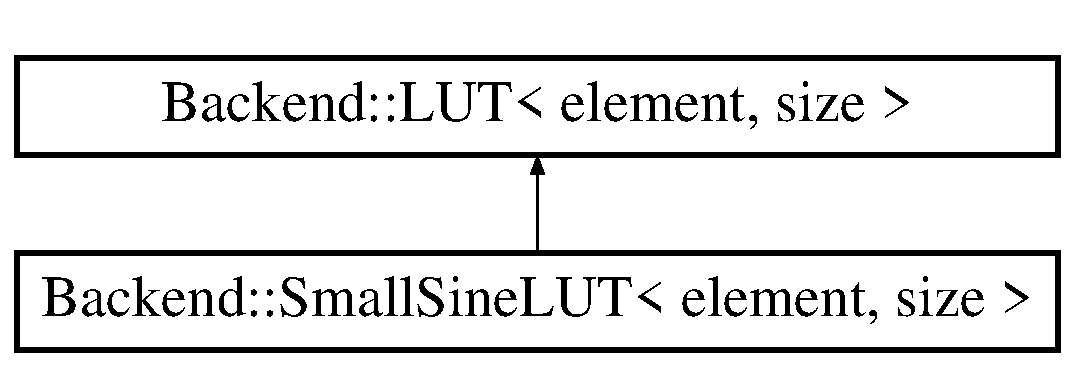
\includegraphics[height=2.000000cm]{classBackend_1_1SmallSineLUT}
\end{center}
\end{figure}
\subsection*{Public Member Functions}
\begin{DoxyCompactItemize}
\item 
\hyperlink{classBackend_1_1SmallSineLUT_aa89687103cd20a258e5623ace804bf09}{Small\+Sine\+L\+U\+T} ()
\item 
virtual \hyperlink{classBackend_1_1SmallSineLUT_a75767a2ebad8a8c4d8a4a54b7c61bb0e}{$\sim$\+Small\+Sine\+L\+U\+T} ()
\item 
virtual element \hyperlink{classBackend_1_1SmallSineLUT_a2b6fdef4f825da7555ca4002f1dd94af}{operator()} (double const \&x)
\item 
element const \& \hyperlink{classBackend_1_1LUT_a9a7c75f36c72778098a091db3269c29c}{operator\mbox{[}$\,$\mbox{]}} (unsigned long const \&index)
\item 
unsigned long const \& \hyperlink{classBackend_1_1LUT_a3ab84f04569e89cd6046da599c6edbae}{Size} () const 
\end{DoxyCompactItemize}
\subsection*{Protected Member Functions}
\begin{DoxyCompactItemize}
\item 
void \hyperlink{classBackend_1_1SmallSineLUT_a981ef95660709f9a796dc176e4c66cf3}{fill} ()
\item 
element const \& \hyperlink{classBackend_1_1SmallSineLUT_ab4403a4852d61cef8199a3f2cb313c57}{lookup} (double index)
\end{DoxyCompactItemize}
\subsection*{Protected Attributes}
\begin{DoxyCompactItemize}
\item 
element \hyperlink{classBackend_1_1LUT_ae70f3f0c9aaa9e0b85517d8e2c61d9a5}{\+\_\+table} \mbox{[}size\mbox{]}
\item 
const unsigned long \hyperlink{classBackend_1_1LUT_a94d2ce1a7c644ce2d4f8e905790b9b54}{\+\_\+size}
\end{DoxyCompactItemize}


\subsection{Detailed Description}
\subsubsection*{template$<$typename element, unsigned long size$>$class Backend\+::\+Small\+Sine\+L\+U\+T$<$ element, size $>$}



Definition at line 48 of file Sine\+L\+U\+T.\+h.



\subsection{Constructor \& Destructor Documentation}
\hypertarget{classBackend_1_1SmallSineLUT_aa89687103cd20a258e5623ace804bf09}{\index{Backend\+::\+Small\+Sine\+L\+U\+T@{Backend\+::\+Small\+Sine\+L\+U\+T}!Small\+Sine\+L\+U\+T@{Small\+Sine\+L\+U\+T}}
\index{Small\+Sine\+L\+U\+T@{Small\+Sine\+L\+U\+T}!Backend\+::\+Small\+Sine\+L\+U\+T@{Backend\+::\+Small\+Sine\+L\+U\+T}}
\subsubsection[{Small\+Sine\+L\+U\+T}]{\setlength{\rightskip}{0pt plus 5cm}template$<$typename element , unsigned long size$>$ {\bf Backend\+::\+Small\+Sine\+L\+U\+T}$<$ element, size $>$\+::{\bf Small\+Sine\+L\+U\+T} (
\begin{DoxyParamCaption}
{}
\end{DoxyParamCaption}
)\hspace{0.3cm}{\ttfamily [inline]}}}\label{classBackend_1_1SmallSineLUT_aa89687103cd20a258e5623ace804bf09}


Definition at line 50 of file Sine\+L\+U\+T.\+h.


\begin{DoxyCode}
50 :LUT<element,size>()\{\hyperlink{classBackend_1_1SmallSineLUT_a981ef95660709f9a796dc176e4c66cf3}{fill}();\}
\end{DoxyCode}
\hypertarget{classBackend_1_1SmallSineLUT_a75767a2ebad8a8c4d8a4a54b7c61bb0e}{\index{Backend\+::\+Small\+Sine\+L\+U\+T@{Backend\+::\+Small\+Sine\+L\+U\+T}!````~Small\+Sine\+L\+U\+T@{$\sim$\+Small\+Sine\+L\+U\+T}}
\index{````~Small\+Sine\+L\+U\+T@{$\sim$\+Small\+Sine\+L\+U\+T}!Backend\+::\+Small\+Sine\+L\+U\+T@{Backend\+::\+Small\+Sine\+L\+U\+T}}
\subsubsection[{$\sim$\+Small\+Sine\+L\+U\+T}]{\setlength{\rightskip}{0pt plus 5cm}template$<$typename element , unsigned long size$>$ virtual {\bf Backend\+::\+Small\+Sine\+L\+U\+T}$<$ element, size $>$\+::$\sim${\bf Small\+Sine\+L\+U\+T} (
\begin{DoxyParamCaption}
{}
\end{DoxyParamCaption}
)\hspace{0.3cm}{\ttfamily [inline]}, {\ttfamily [virtual]}}}\label{classBackend_1_1SmallSineLUT_a75767a2ebad8a8c4d8a4a54b7c61bb0e}


Definition at line 51 of file Sine\+L\+U\+T.\+h.


\begin{DoxyCode}
51 \{\}
\end{DoxyCode}


\subsection{Member Function Documentation}
\hypertarget{classBackend_1_1SmallSineLUT_a981ef95660709f9a796dc176e4c66cf3}{\index{Backend\+::\+Small\+Sine\+L\+U\+T@{Backend\+::\+Small\+Sine\+L\+U\+T}!fill@{fill}}
\index{fill@{fill}!Backend\+::\+Small\+Sine\+L\+U\+T@{Backend\+::\+Small\+Sine\+L\+U\+T}}
\subsubsection[{fill}]{\setlength{\rightskip}{0pt plus 5cm}template$<$typename element , unsigned long size$>$ void {\bf Backend\+::\+Small\+Sine\+L\+U\+T}$<$ element, size $>$\+::fill (
\begin{DoxyParamCaption}
{}
\end{DoxyParamCaption}
)\hspace{0.3cm}{\ttfamily [inline]}, {\ttfamily [protected]}}}\label{classBackend_1_1SmallSineLUT_a981ef95660709f9a796dc176e4c66cf3}


Definition at line 74 of file Sine\+L\+U\+T.\+h.


\begin{DoxyCode}
74                           \{
75             \textcolor{keywordtype}{double} step = (M\_PI\_2/this->\hyperlink{classBackend_1_1LUT_a94d2ce1a7c644ce2d4f8e905790b9b54}{\_size});
76             \textcolor{keywordtype}{double} phs=0;
77             \textcolor{keywordflow}{for} (\textcolor{keywordtype}{int} i=0; i<this->\hyperlink{classBackend_1_1LUT_a94d2ce1a7c644ce2d4f8e905790b9b54}{\_size}; ++i) \{
78                 this->\hyperlink{classBackend_1_1LUT_ae70f3f0c9aaa9e0b85517d8e2c61d9a5}{\_table}[i] = sin(phs);
79                 phs+=step;
80             \}
81         \}
\end{DoxyCode}
\hypertarget{classBackend_1_1SmallSineLUT_ab4403a4852d61cef8199a3f2cb313c57}{\index{Backend\+::\+Small\+Sine\+L\+U\+T@{Backend\+::\+Small\+Sine\+L\+U\+T}!lookup@{lookup}}
\index{lookup@{lookup}!Backend\+::\+Small\+Sine\+L\+U\+T@{Backend\+::\+Small\+Sine\+L\+U\+T}}
\subsubsection[{lookup}]{\setlength{\rightskip}{0pt plus 5cm}template$<$typename element , unsigned long size$>$ element const\& {\bf Backend\+::\+Small\+Sine\+L\+U\+T}$<$ element, size $>$\+::lookup (
\begin{DoxyParamCaption}
\item[{double}]{index}
\end{DoxyParamCaption}
)\hspace{0.3cm}{\ttfamily [inline]}, {\ttfamily [protected]}}}\label{classBackend_1_1SmallSineLUT_ab4403a4852d61cef8199a3f2cb313c57}


Definition at line 82 of file Sine\+L\+U\+T.\+h.


\begin{DoxyCode}
82                                                   \{
83             \textcolor{comment}{//possibvly interpolate for better quality}
84             \textcolor{keywordflow}{return} this->\hyperlink{classBackend_1_1LUT_ae70f3f0c9aaa9e0b85517d8e2c61d9a5}{\_table}[(unsigned)(index* (this->\hyperlink{classBackend_1_1LUT_a94d2ce1a7c644ce2d4f8e905790b9b54}{\_size}-1))];
85         \}
\end{DoxyCode}
\hypertarget{classBackend_1_1SmallSineLUT_a2b6fdef4f825da7555ca4002f1dd94af}{\index{Backend\+::\+Small\+Sine\+L\+U\+T@{Backend\+::\+Small\+Sine\+L\+U\+T}!operator()@{operator()}}
\index{operator()@{operator()}!Backend\+::\+Small\+Sine\+L\+U\+T@{Backend\+::\+Small\+Sine\+L\+U\+T}}
\subsubsection[{operator()}]{\setlength{\rightskip}{0pt plus 5cm}template$<$typename element , unsigned long size$>$ virtual element {\bf Backend\+::\+Small\+Sine\+L\+U\+T}$<$ element, size $>$\+::operator() (
\begin{DoxyParamCaption}
\item[{double const \&}]{x}
\end{DoxyParamCaption}
)\hspace{0.3cm}{\ttfamily [inline]}, {\ttfamily [virtual]}}}\label{classBackend_1_1SmallSineLUT_a2b6fdef4f825da7555ca4002f1dd94af}


Reimplemented from \hyperlink{classBackend_1_1LUT_aea3420a7a3552f38ba8f9ea979bab764}{Backend\+::\+L\+U\+T$<$ element, size $>$}.



Definition at line 52 of file Sine\+L\+U\+T.\+h.


\begin{DoxyCode}
52                                                           \{
53             \textcolor{keywordtype}{double} phs=x;
54             \textcolor{comment}{//need range checking on x to ensure 0-1 range}
55             phs=fabs(phs);
56             phs=phs-((int)phs);
57             \textcolor{keywordflow}{if} (phs>=0.0 && phs<=0.25) \{
58                 \textcolor{comment}{//sin(x) = sin(x)}
59                 \textcolor{keywordflow}{return} \hyperlink{classBackend_1_1SmallSineLUT_ab4403a4852d61cef8199a3f2cb313c57}{lookup}(phs*4);
60             \}\textcolor{keywordflow}{else} \textcolor{keywordflow}{if} (phs>0.25 && phs<=0.5)\{
61                 \textcolor{comment}{//sin(x) =      sin(pi-x). We are working in 0-1 range not 0-2pi so 0.5 is substituted for
       pi}
62                 \textcolor{keywordflow}{return} \hyperlink{classBackend_1_1SmallSineLUT_ab4403a4852d61cef8199a3f2cb313c57}{lookup}(2-(phs*4));
63             \}\textcolor{keywordflow}{else} \textcolor{keywordflow}{if} (phs>0.5 && phs<=0.75)\{
64                 \textcolor{comment}{//sin(x)=-sin(pi+x);}
65                 \textcolor{keywordflow}{return} -\hyperlink{classBackend_1_1SmallSineLUT_ab4403a4852d61cef8199a3f2cb313c57}{lookup}((phs*4)-2);
66             \}\textcolor{keywordflow}{else} \textcolor{keywordflow}{if} (phs>0.75 && phs<=1.0)\{
67                 \textcolor{comment}{//sin(x) = -sin(-x)}
68                 \textcolor{keywordflow}{return} -\hyperlink{classBackend_1_1SmallSineLUT_ab4403a4852d61cef8199a3f2cb313c57}{lookup}(4-(phs*4));
69             \}
70             
71             \textcolor{keywordflow}{return} 0;
72         \}
\end{DoxyCode}
\hypertarget{classBackend_1_1LUT_a9a7c75f36c72778098a091db3269c29c}{\index{Backend\+::\+Small\+Sine\+L\+U\+T@{Backend\+::\+Small\+Sine\+L\+U\+T}!operator\mbox{[}$\,$\mbox{]}@{operator[]}}
\index{operator\mbox{[}$\,$\mbox{]}@{operator[]}!Backend\+::\+Small\+Sine\+L\+U\+T@{Backend\+::\+Small\+Sine\+L\+U\+T}}
\subsubsection[{operator[]}]{\setlength{\rightskip}{0pt plus 5cm}template$<$typename element, unsigned long size$>$ element const\& {\bf Backend\+::\+L\+U\+T}$<$ element, size $>$\+::operator\mbox{[}$\,$\mbox{]} (
\begin{DoxyParamCaption}
\item[{unsigned long const \&}]{index}
\end{DoxyParamCaption}
)\hspace{0.3cm}{\ttfamily [inline]}, {\ttfamily [inherited]}}}\label{classBackend_1_1LUT_a9a7c75f36c72778098a091db3269c29c}


Definition at line 22 of file L\+U\+T.\+h.


\begin{DoxyCode}
22                                                              \{
23 \textcolor{preprocessor}{#ifdef DEBUG}
24             assert(index<\hyperlink{classBackend_1_1LUT_a94d2ce1a7c644ce2d4f8e905790b9b54}{\_size});
25 \textcolor{preprocessor}{#endif}
26             \textcolor{keywordflow}{return} \hyperlink{classBackend_1_1LUT_ae70f3f0c9aaa9e0b85517d8e2c61d9a5}{\_table}[index];
27         \}
\end{DoxyCode}
\hypertarget{classBackend_1_1LUT_a3ab84f04569e89cd6046da599c6edbae}{\index{Backend\+::\+Small\+Sine\+L\+U\+T@{Backend\+::\+Small\+Sine\+L\+U\+T}!Size@{Size}}
\index{Size@{Size}!Backend\+::\+Small\+Sine\+L\+U\+T@{Backend\+::\+Small\+Sine\+L\+U\+T}}
\subsubsection[{Size}]{\setlength{\rightskip}{0pt plus 5cm}template$<$typename element, unsigned long size$>$ unsigned long const\& {\bf Backend\+::\+L\+U\+T}$<$ element, size $>$\+::Size (
\begin{DoxyParamCaption}
{}
\end{DoxyParamCaption}
) const\hspace{0.3cm}{\ttfamily [inline]}, {\ttfamily [inherited]}}}\label{classBackend_1_1LUT_a3ab84f04569e89cd6046da599c6edbae}


Definition at line 31 of file L\+U\+T.\+h.


\begin{DoxyCode}
31                                         \{
32             \textcolor{keywordflow}{return} \hyperlink{classBackend_1_1LUT_a94d2ce1a7c644ce2d4f8e905790b9b54}{\_size};
33         \}
\end{DoxyCode}


\subsection{Member Data Documentation}
\hypertarget{classBackend_1_1LUT_a94d2ce1a7c644ce2d4f8e905790b9b54}{\index{Backend\+::\+Small\+Sine\+L\+U\+T@{Backend\+::\+Small\+Sine\+L\+U\+T}!\+\_\+size@{\+\_\+size}}
\index{\+\_\+size@{\+\_\+size}!Backend\+::\+Small\+Sine\+L\+U\+T@{Backend\+::\+Small\+Sine\+L\+U\+T}}
\subsubsection[{\+\_\+size}]{\setlength{\rightskip}{0pt plus 5cm}template$<$typename element, unsigned long size$>$ const unsigned long {\bf Backend\+::\+L\+U\+T}$<$ element, size $>$\+::\+\_\+size\hspace{0.3cm}{\ttfamily [protected]}, {\ttfamily [inherited]}}}\label{classBackend_1_1LUT_a94d2ce1a7c644ce2d4f8e905790b9b54}


Definition at line 36 of file L\+U\+T.\+h.

\hypertarget{classBackend_1_1LUT_ae70f3f0c9aaa9e0b85517d8e2c61d9a5}{\index{Backend\+::\+Small\+Sine\+L\+U\+T@{Backend\+::\+Small\+Sine\+L\+U\+T}!\+\_\+table@{\+\_\+table}}
\index{\+\_\+table@{\+\_\+table}!Backend\+::\+Small\+Sine\+L\+U\+T@{Backend\+::\+Small\+Sine\+L\+U\+T}}
\subsubsection[{\+\_\+table}]{\setlength{\rightskip}{0pt plus 5cm}template$<$typename element, unsigned long size$>$ element {\bf Backend\+::\+L\+U\+T}$<$ element, size $>$\+::\+\_\+table\mbox{[}size\mbox{]}\hspace{0.3cm}{\ttfamily [protected]}, {\ttfamily [inherited]}}}\label{classBackend_1_1LUT_ae70f3f0c9aaa9e0b85517d8e2c61d9a5}


Definition at line 35 of file L\+U\+T.\+h.



The documentation for this class was generated from the following file\+:\begin{DoxyCompactItemize}
\item 
/\+Users/alexanderzywicki/\+Documents/\+School\+\_\+\+Stuff/\+Fall\+\_\+2014/\+Digital\+\_\+\+Signal\+\_\+\+Generation\+\_\+and\+\_\+\+Analysis/src/include/\hyperlink{SineLUT_8h}{Sine\+L\+U\+T.\+h}\end{DoxyCompactItemize}

\hypertarget{classBackend_1_1SmallSineLUT_3_01int32__t_00_01size_01_4}{\section{Backend\+:\+:Small\+Sine\+L\+U\+T$<$ int32\+\_\+t, size $>$ Class Template Reference}
\label{classBackend_1_1SmallSineLUT_3_01int32__t_00_01size_01_4}\index{Backend\+::\+Small\+Sine\+L\+U\+T$<$ int32\+\_\+t, size $>$@{Backend\+::\+Small\+Sine\+L\+U\+T$<$ int32\+\_\+t, size $>$}}
}


{\ttfamily \#include $<$Sine\+L\+U\+T.\+h$>$}

Inheritance diagram for Backend\+:\+:Small\+Sine\+L\+U\+T$<$ int32\+\_\+t, size $>$\+:\begin{figure}[H]
\begin{center}
\leavevmode
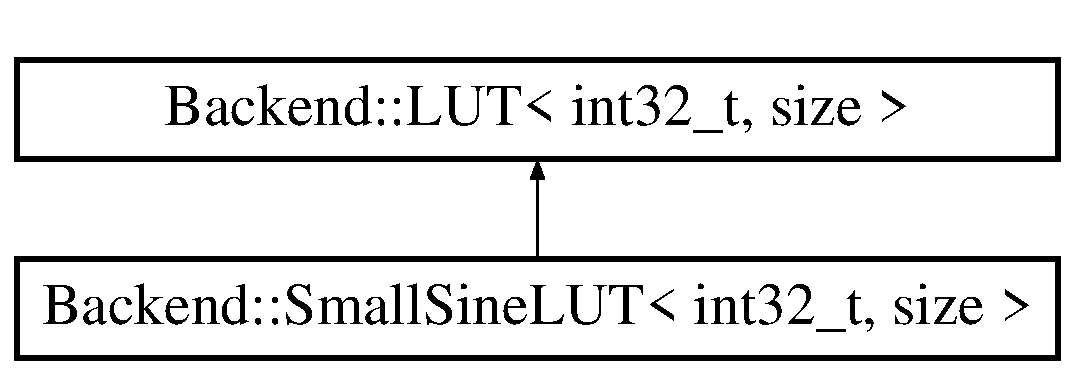
\includegraphics[height=2.000000cm]{classBackend_1_1SmallSineLUT_3_01int32__t_00_01size_01_4}
\end{center}
\end{figure}
\subsection*{Public Member Functions}
\begin{DoxyCompactItemize}
\item 
\hyperlink{classBackend_1_1SmallSineLUT_3_01int32__t_00_01size_01_4_a05f2fcd7c8a0430dc0137e67d385dc1b}{Small\+Sine\+L\+U\+T} ()
\item 
virtual \hyperlink{classBackend_1_1SmallSineLUT_3_01int32__t_00_01size_01_4_a3db4fc45b900c846711e0cbd828dbbf4}{$\sim$\+Small\+Sine\+L\+U\+T} ()
\item 
virtual int32\+\_\+t \hyperlink{classBackend_1_1SmallSineLUT_3_01int32__t_00_01size_01_4_a7eff39a75385950b722ed2ba7140d4e4}{operator()} (double const \&x)
\item 
int32\+\_\+tconst \& \hyperlink{classBackend_1_1LUT_a9a7c75f36c72778098a091db3269c29c}{operator\mbox{[}$\,$\mbox{]}} (unsigned long const \&index)
\item 
unsigned long const \& \hyperlink{classBackend_1_1LUT_a3ab84f04569e89cd6046da599c6edbae}{Size} () const
\end{DoxyCompactItemize}
\subsection*{Protected Member Functions}
\begin{DoxyCompactItemize}
\item 
void \hyperlink{classBackend_1_1SmallSineLUT_3_01int32__t_00_01size_01_4_a0fad3b2c0904d1c2a65c850431f1ac3f}{fill} ()
\item 
int32\+\_\+t const \& \hyperlink{classBackend_1_1SmallSineLUT_3_01int32__t_00_01size_01_4_ab58e1db04772d8fad7b5d0f4936454bd}{lookup} (double \&\&index)
\end{DoxyCompactItemize}
\subsection*{Protected Attributes}
\begin{DoxyCompactItemize}
\item 
int32\+\_\+t \hyperlink{classBackend_1_1LUT_ae70f3f0c9aaa9e0b85517d8e2c61d9a5}{\+\_\+table} \mbox{[}size\mbox{]}
\item 
const unsigned long \hyperlink{classBackend_1_1LUT_a94d2ce1a7c644ce2d4f8e905790b9b54}{\+\_\+size}
\end{DoxyCompactItemize}


\subsection{Detailed Description}
\subsubsection*{template$<$unsigned long size$>$class Backend\+::\+Small\+Sine\+L\+U\+T$<$ int32\+\_\+t, size $>$}



Definition at line 91 of file Sine\+L\+U\+T.\+h.



\subsection{Constructor \& Destructor Documentation}
\hypertarget{classBackend_1_1SmallSineLUT_3_01int32__t_00_01size_01_4_a05f2fcd7c8a0430dc0137e67d385dc1b}{\index{Backend\+::\+Small\+Sine\+L\+U\+T$<$ int32\+\_\+t, size $>$@{Backend\+::\+Small\+Sine\+L\+U\+T$<$ int32\+\_\+t, size $>$}!Small\+Sine\+L\+U\+T@{Small\+Sine\+L\+U\+T}}
\index{Small\+Sine\+L\+U\+T@{Small\+Sine\+L\+U\+T}!Backend\+::\+Small\+Sine\+L\+U\+T$<$ int32\+\_\+t, size $>$@{Backend\+::\+Small\+Sine\+L\+U\+T$<$ int32\+\_\+t, size $>$}}
\subsubsection[{Small\+Sine\+L\+U\+T}]{\setlength{\rightskip}{0pt plus 5cm}template$<$unsigned long size$>$ {\bf Backend\+::\+Small\+Sine\+L\+U\+T}$<$ int32\+\_\+t, size $>$\+::{\bf Small\+Sine\+L\+U\+T} (
\begin{DoxyParamCaption}
{}
\end{DoxyParamCaption}
)\hspace{0.3cm}{\ttfamily [inline]}}}\label{classBackend_1_1SmallSineLUT_3_01int32__t_00_01size_01_4_a05f2fcd7c8a0430dc0137e67d385dc1b}


Definition at line 93 of file Sine\+L\+U\+T.\+h.


\begin{DoxyCode}
93 :LUT<int32\_t,size>()\{\hyperlink{classBackend_1_1SmallSineLUT_3_01int32__t_00_01size_01_4_a0fad3b2c0904d1c2a65c850431f1ac3f}{fill}();\}
\end{DoxyCode}
\hypertarget{classBackend_1_1SmallSineLUT_3_01int32__t_00_01size_01_4_a3db4fc45b900c846711e0cbd828dbbf4}{\index{Backend\+::\+Small\+Sine\+L\+U\+T$<$ int32\+\_\+t, size $>$@{Backend\+::\+Small\+Sine\+L\+U\+T$<$ int32\+\_\+t, size $>$}!````~Small\+Sine\+L\+U\+T@{$\sim$\+Small\+Sine\+L\+U\+T}}
\index{````~Small\+Sine\+L\+U\+T@{$\sim$\+Small\+Sine\+L\+U\+T}!Backend\+::\+Small\+Sine\+L\+U\+T$<$ int32\+\_\+t, size $>$@{Backend\+::\+Small\+Sine\+L\+U\+T$<$ int32\+\_\+t, size $>$}}
\subsubsection[{$\sim$\+Small\+Sine\+L\+U\+T}]{\setlength{\rightskip}{0pt plus 5cm}template$<$unsigned long size$>$ virtual {\bf Backend\+::\+Small\+Sine\+L\+U\+T}$<$ int32\+\_\+t, size $>$\+::$\sim${\bf Small\+Sine\+L\+U\+T} (
\begin{DoxyParamCaption}
{}
\end{DoxyParamCaption}
)\hspace{0.3cm}{\ttfamily [inline]}, {\ttfamily [virtual]}}}\label{classBackend_1_1SmallSineLUT_3_01int32__t_00_01size_01_4_a3db4fc45b900c846711e0cbd828dbbf4}


Definition at line 94 of file Sine\+L\+U\+T.\+h.


\begin{DoxyCode}
94 \{\}
\end{DoxyCode}


\subsection{Member Function Documentation}
\hypertarget{classBackend_1_1SmallSineLUT_3_01int32__t_00_01size_01_4_a0fad3b2c0904d1c2a65c850431f1ac3f}{\index{Backend\+::\+Small\+Sine\+L\+U\+T$<$ int32\+\_\+t, size $>$@{Backend\+::\+Small\+Sine\+L\+U\+T$<$ int32\+\_\+t, size $>$}!fill@{fill}}
\index{fill@{fill}!Backend\+::\+Small\+Sine\+L\+U\+T$<$ int32\+\_\+t, size $>$@{Backend\+::\+Small\+Sine\+L\+U\+T$<$ int32\+\_\+t, size $>$}}
\subsubsection[{fill}]{\setlength{\rightskip}{0pt plus 5cm}template$<$unsigned long size$>$ void {\bf Backend\+::\+Small\+Sine\+L\+U\+T}$<$ int32\+\_\+t, size $>$\+::fill (
\begin{DoxyParamCaption}
{}
\end{DoxyParamCaption}
)\hspace{0.3cm}{\ttfamily [inline]}, {\ttfamily [protected]}}}\label{classBackend_1_1SmallSineLUT_3_01int32__t_00_01size_01_4_a0fad3b2c0904d1c2a65c850431f1ac3f}


Definition at line 121 of file Sine\+L\+U\+T.\+h.


\begin{DoxyCode}
121                           \{
122             \textcolor{keywordtype}{double} step = (M\_PI\_2/this->\hyperlink{classBackend_1_1LUT_a94d2ce1a7c644ce2d4f8e905790b9b54}{\_size});
123             \textcolor{keywordtype}{double} phs=0;
124             \textcolor{keywordtype}{double} scale = pow(2, \textcolor{keyword}{sizeof}(int32\_t)*8)*0.5;
125             \textcolor{keywordflow}{for} (int32\_t i=0; i<this->\hyperlink{classBackend_1_1LUT_a94d2ce1a7c644ce2d4f8e905790b9b54}{\_size}; ++i) \{
126                 this->\hyperlink{classBackend_1_1LUT_ae70f3f0c9aaa9e0b85517d8e2c61d9a5}{\_table}[i] = sin(phs)*scale;
127                 phs+=step;
128             \}
129         \}
\end{DoxyCode}
\hypertarget{classBackend_1_1SmallSineLUT_3_01int32__t_00_01size_01_4_ab58e1db04772d8fad7b5d0f4936454bd}{\index{Backend\+::\+Small\+Sine\+L\+U\+T$<$ int32\+\_\+t, size $>$@{Backend\+::\+Small\+Sine\+L\+U\+T$<$ int32\+\_\+t, size $>$}!lookup@{lookup}}
\index{lookup@{lookup}!Backend\+::\+Small\+Sine\+L\+U\+T$<$ int32\+\_\+t, size $>$@{Backend\+::\+Small\+Sine\+L\+U\+T$<$ int32\+\_\+t, size $>$}}
\subsubsection[{lookup}]{\setlength{\rightskip}{0pt plus 5cm}template$<$unsigned long size$>$ int32\+\_\+t const\& {\bf Backend\+::\+Small\+Sine\+L\+U\+T}$<$ int32\+\_\+t, size $>$\+::lookup (
\begin{DoxyParamCaption}
\item[{double \&\&}]{index}
\end{DoxyParamCaption}
)\hspace{0.3cm}{\ttfamily [inline]}, {\ttfamily [protected]}}}\label{classBackend_1_1SmallSineLUT_3_01int32__t_00_01size_01_4_ab58e1db04772d8fad7b5d0f4936454bd}


Definition at line 130 of file Sine\+L\+U\+T.\+h.


\begin{DoxyCode}
130                                                     \{
131             \textcolor{comment}{//possibvly interpolate for better quality}
132             \textcolor{keywordflow}{return} this->\hyperlink{classBackend_1_1LUT_ae70f3f0c9aaa9e0b85517d8e2c61d9a5}{\_table}[(unsigned)(index* (this->\hyperlink{classBackend_1_1LUT_a94d2ce1a7c644ce2d4f8e905790b9b54}{\_size}-1))];
133         \}
\end{DoxyCode}
\hypertarget{classBackend_1_1SmallSineLUT_3_01int32__t_00_01size_01_4_a7eff39a75385950b722ed2ba7140d4e4}{\index{Backend\+::\+Small\+Sine\+L\+U\+T$<$ int32\+\_\+t, size $>$@{Backend\+::\+Small\+Sine\+L\+U\+T$<$ int32\+\_\+t, size $>$}!operator()@{operator()}}
\index{operator()@{operator()}!Backend\+::\+Small\+Sine\+L\+U\+T$<$ int32\+\_\+t, size $>$@{Backend\+::\+Small\+Sine\+L\+U\+T$<$ int32\+\_\+t, size $>$}}
\subsubsection[{operator()}]{\setlength{\rightskip}{0pt plus 5cm}template$<$unsigned long size$>$ virtual int32\+\_\+t {\bf Backend\+::\+Small\+Sine\+L\+U\+T}$<$ int32\+\_\+t, size $>$\+::operator() (
\begin{DoxyParamCaption}
\item[{double const \&}]{x}
\end{DoxyParamCaption}
)\hspace{0.3cm}{\ttfamily [inline]}, {\ttfamily [virtual]}}}\label{classBackend_1_1SmallSineLUT_3_01int32__t_00_01size_01_4_a7eff39a75385950b722ed2ba7140d4e4}


Reimplemented from \hyperlink{classBackend_1_1LUT_aea3420a7a3552f38ba8f9ea979bab764}{Backend\+::\+L\+U\+T$<$ int32\+\_\+t, size $>$}.



Definition at line 95 of file Sine\+L\+U\+T.\+h.


\begin{DoxyCode}
95                                                           \{
96             \textcolor{keywordtype}{double} phs=x;
97             \textcolor{comment}{//need range checking on x to ensure 0-1 range}
98             phs=fabs(phs);
99             phs=phs-((int32\_t)phs);
100             \textcolor{keywordflow}{if} (phs>=0.0 && phs<=0.25) \{
101                 \textcolor{comment}{//sin(x) = sin(x)}
102                 \textcolor{keywordflow}{return} \hyperlink{classBackend_1_1SmallSineLUT_3_01int32__t_00_01size_01_4_ab58e1db04772d8fad7b5d0f4936454bd}{lookup}(phs*4);
103                 
104             \}\textcolor{keywordflow}{else} \textcolor{keywordflow}{if} (phs>0.25 && phs<=0.5)\{
105                 \textcolor{comment}{//sin(x) =      sin(pi-x). We are working in 0-1 range not 0-2pi so 0.5 is substituted for
       pi}
106                 \textcolor{keywordflow}{return} \hyperlink{classBackend_1_1SmallSineLUT_3_01int32__t_00_01size_01_4_ab58e1db04772d8fad7b5d0f4936454bd}{lookup}(2-(phs*4));
107             \}\textcolor{keywordflow}{else} \textcolor{keywordflow}{if} (phs>0.5 && phs<=0.75)\{
108                 \textcolor{comment}{//sin(x)=-sin(pi+x);}
109                 \textcolor{keywordflow}{return} -\hyperlink{classBackend_1_1SmallSineLUT_3_01int32__t_00_01size_01_4_ab58e1db04772d8fad7b5d0f4936454bd}{lookup}((phs*4)-2);
110             \}\textcolor{keywordflow}{else} \textcolor{keywordflow}{if} (phs>0.75 && phs<=1.0)\{
111                 \textcolor{comment}{//sin(x) = -sin(-x)}
112                 \textcolor{keywordflow}{return} -\hyperlink{classBackend_1_1SmallSineLUT_3_01int32__t_00_01size_01_4_ab58e1db04772d8fad7b5d0f4936454bd}{lookup}(4-(phs*4));
113                 
114             \}\textcolor{keywordflow}{else}\{
115                 
116             \}
117             
118             \textcolor{keywordflow}{return} 0;
119         \}
\end{DoxyCode}
\hypertarget{classBackend_1_1LUT_a9a7c75f36c72778098a091db3269c29c}{\index{Backend\+::\+Small\+Sine\+L\+U\+T$<$ int32\+\_\+t, size $>$@{Backend\+::\+Small\+Sine\+L\+U\+T$<$ int32\+\_\+t, size $>$}!operator\mbox{[}$\,$\mbox{]}@{operator[]}}
\index{operator\mbox{[}$\,$\mbox{]}@{operator[]}!Backend\+::\+Small\+Sine\+L\+U\+T$<$ int32\+\_\+t, size $>$@{Backend\+::\+Small\+Sine\+L\+U\+T$<$ int32\+\_\+t, size $>$}}
\subsubsection[{operator[]}]{\setlength{\rightskip}{0pt plus 5cm}int32\+\_\+t  const\& {\bf Backend\+::\+L\+U\+T}$<$ int32\+\_\+t , size $>$\+::operator\mbox{[}$\,$\mbox{]} (
\begin{DoxyParamCaption}
\item[{unsigned long const \&}]{index}
\end{DoxyParamCaption}
)\hspace{0.3cm}{\ttfamily [inline]}, {\ttfamily [inherited]}}}\label{classBackend_1_1LUT_a9a7c75f36c72778098a091db3269c29c}


Definition at line 22 of file L\+U\+T.\+h.


\begin{DoxyCode}
22                                                              \{
23 \textcolor{preprocessor}{#ifdef DEBUG}
24             assert(index<\hyperlink{classBackend_1_1LUT_a94d2ce1a7c644ce2d4f8e905790b9b54}{\_size});
25 \textcolor{preprocessor}{#endif}
26             \textcolor{keywordflow}{return} \hyperlink{classBackend_1_1LUT_ae70f3f0c9aaa9e0b85517d8e2c61d9a5}{\_table}[index];
27         \}
\end{DoxyCode}
\hypertarget{classBackend_1_1LUT_a3ab84f04569e89cd6046da599c6edbae}{\index{Backend\+::\+Small\+Sine\+L\+U\+T$<$ int32\+\_\+t, size $>$@{Backend\+::\+Small\+Sine\+L\+U\+T$<$ int32\+\_\+t, size $>$}!Size@{Size}}
\index{Size@{Size}!Backend\+::\+Small\+Sine\+L\+U\+T$<$ int32\+\_\+t, size $>$@{Backend\+::\+Small\+Sine\+L\+U\+T$<$ int32\+\_\+t, size $>$}}
\subsubsection[{Size}]{\setlength{\rightskip}{0pt plus 5cm}unsigned long const\& {\bf Backend\+::\+L\+U\+T}$<$ int32\+\_\+t , size $>$\+::Size (
\begin{DoxyParamCaption}
{}
\end{DoxyParamCaption}
) const\hspace{0.3cm}{\ttfamily [inline]}, {\ttfamily [inherited]}}}\label{classBackend_1_1LUT_a3ab84f04569e89cd6046da599c6edbae}


Definition at line 31 of file L\+U\+T.\+h.


\begin{DoxyCode}
31                                         \{
32             \textcolor{keywordflow}{return} \hyperlink{classBackend_1_1LUT_a94d2ce1a7c644ce2d4f8e905790b9b54}{\_size};
33         \}
\end{DoxyCode}


\subsection{Member Data Documentation}
\hypertarget{classBackend_1_1LUT_a94d2ce1a7c644ce2d4f8e905790b9b54}{\index{Backend\+::\+Small\+Sine\+L\+U\+T$<$ int32\+\_\+t, size $>$@{Backend\+::\+Small\+Sine\+L\+U\+T$<$ int32\+\_\+t, size $>$}!\+\_\+size@{\+\_\+size}}
\index{\+\_\+size@{\+\_\+size}!Backend\+::\+Small\+Sine\+L\+U\+T$<$ int32\+\_\+t, size $>$@{Backend\+::\+Small\+Sine\+L\+U\+T$<$ int32\+\_\+t, size $>$}}
\subsubsection[{\+\_\+size}]{\setlength{\rightskip}{0pt plus 5cm}const unsigned long {\bf Backend\+::\+L\+U\+T}$<$ int32\+\_\+t , size $>$\+::\+\_\+size\hspace{0.3cm}{\ttfamily [protected]}, {\ttfamily [inherited]}}}\label{classBackend_1_1LUT_a94d2ce1a7c644ce2d4f8e905790b9b54}


Definition at line 36 of file L\+U\+T.\+h.

\hypertarget{classBackend_1_1LUT_ae70f3f0c9aaa9e0b85517d8e2c61d9a5}{\index{Backend\+::\+Small\+Sine\+L\+U\+T$<$ int32\+\_\+t, size $>$@{Backend\+::\+Small\+Sine\+L\+U\+T$<$ int32\+\_\+t, size $>$}!\+\_\+table@{\+\_\+table}}
\index{\+\_\+table@{\+\_\+table}!Backend\+::\+Small\+Sine\+L\+U\+T$<$ int32\+\_\+t, size $>$@{Backend\+::\+Small\+Sine\+L\+U\+T$<$ int32\+\_\+t, size $>$}}
\subsubsection[{\+\_\+table}]{\setlength{\rightskip}{0pt plus 5cm}int32\+\_\+t  {\bf Backend\+::\+L\+U\+T}$<$ int32\+\_\+t , size $>$\+::\+\_\+table\mbox{[}size\mbox{]}\hspace{0.3cm}{\ttfamily [protected]}, {\ttfamily [inherited]}}}\label{classBackend_1_1LUT_ae70f3f0c9aaa9e0b85517d8e2c61d9a5}


Definition at line 35 of file L\+U\+T.\+h.



The documentation for this class was generated from the following file\+:\begin{DoxyCompactItemize}
\item 
/\+Users/alexanderzywicki/\+Documents/\+School\+\_\+\+Stuff/\+Fall\+\_\+2014/\+Digital\+\_\+\+Signal\+\_\+\+Generation\+\_\+and\+\_\+\+Analysis/src/include/\hyperlink{SineLUT_8h}{Sine\+L\+U\+T.\+h}\end{DoxyCompactItemize}

\hypertarget{classSignal_1_1Square}{\section{Signal\+:\+:Square Class Reference}
\label{classSignal_1_1Square}\index{Signal\+::\+Square@{Signal\+::\+Square}}
}


{\ttfamily \#include $<$Square.\+h$>$}

Inheritance diagram for Signal\+:\+:Square\+:\begin{figure}[H]
\begin{center}
\leavevmode
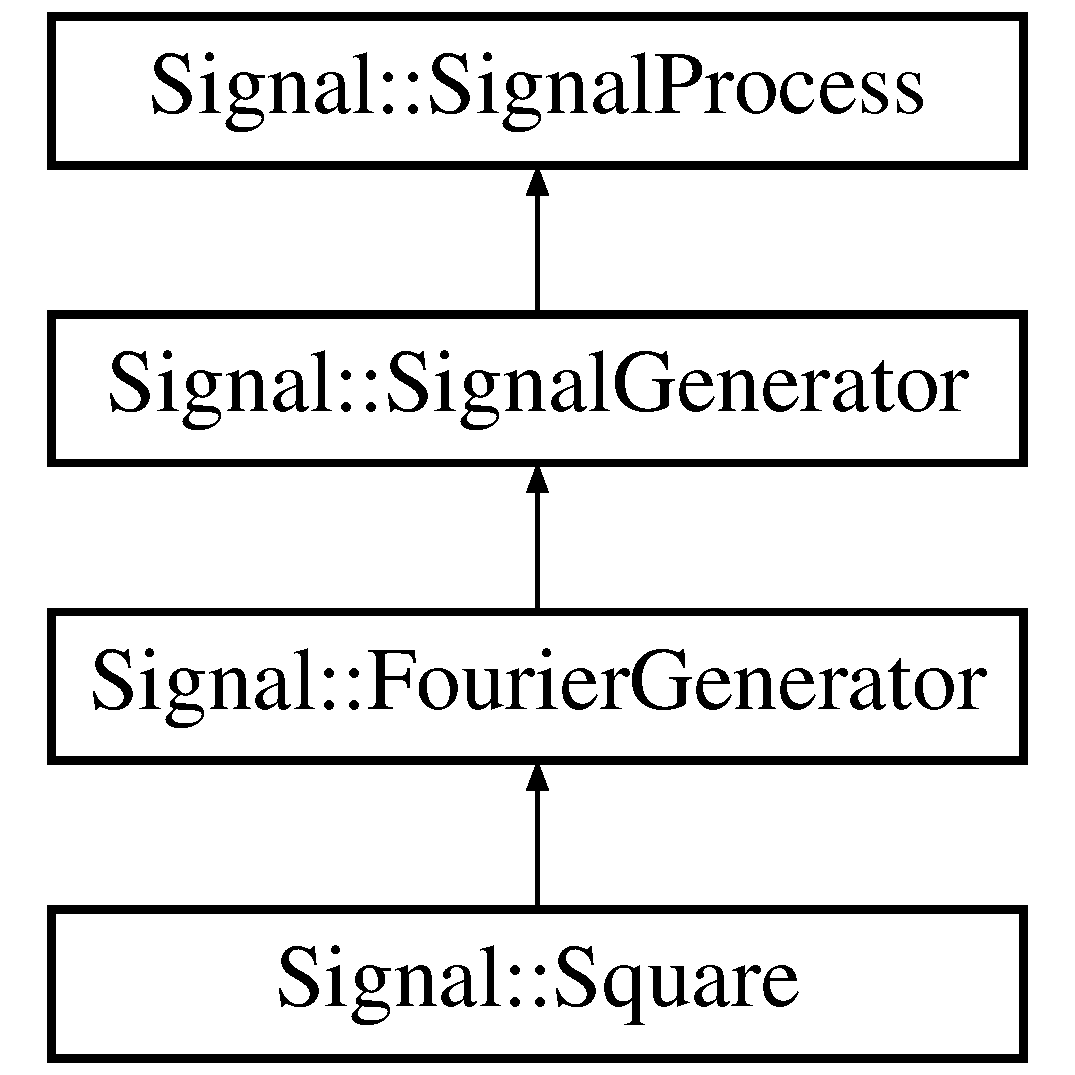
\includegraphics[height=4.000000cm]{classSignal_1_1Square}
\end{center}
\end{figure}
\subsection*{Public Member Functions}
\begin{DoxyCompactItemize}
\item 
\hyperlink{classSignal_1_1Square_a7f26603d620762e80c72de9750f6a7fc}{Square} ()
\item 
\hyperlink{classSignal_1_1Square_af0ead34823fa035db3aa1bcf39116a46}{Square} (double const \&frequency, double const \&phase\+\_\+offset)
\item 
virtual \hyperlink{classSignal_1_1Square_a2eda1d209b2c919a3ce4ff40f2f9fed4}{$\sim$\+Square} ()
\item 
virtual bool \hyperlink{classSignal_1_1Square_a584e1b867aed4cc4a808d8fb844387bc}{Perform} (\hyperlink{classSignal_1_1Sample}{Sample} \&signal)
\item 
virtual bool \hyperlink{classSignal_1_1Square_ab398eba1087030249d04f27a364f45ed}{Perform} (\hyperlink{classSignal_1_1RingBuffer}{Ring\+Buffer} \&signal)
\item 
virtual double const \& \hyperlink{classSignal_1_1Square_a19f966d5b1800f5487cdd164747b21c0}{Frequency} (double const \&value)
\item 
virtual double const \& \hyperlink{classSignal_1_1Square_a49e8516818f89e05ad19dc09b2531e96}{Frequency} ()
\item 
virtual double const \& \hyperlink{classSignal_1_1SignalGenerator_a96af42ee68f94e9b04d034fd68b73ecd}{Frequency} () const 
\item 
virtual double const \& \hyperlink{classSignal_1_1SignalGenerator_ac2538ec946f001e394d2416fda698d1c}{Phase\+Offset} () const 
\item 
virtual double const \& \hyperlink{classSignal_1_1SignalGenerator_ac6a103ff72beaa338f6d18c812522d78}{Phase\+Offset} (double const \&value)
\end{DoxyCompactItemize}
\subsection*{Protected Member Functions}
\begin{DoxyCompactItemize}
\item 
unsigned long \hyperlink{classSignal_1_1FourierGenerator_abfa6ecda1b94d8ae433e0722e4ec092b}{\+\_\+max\+Harms} (double \+\_\+frq)
\item 
double \hyperlink{classSignal_1_1FourierGenerator_aed4334ef6ec8a47f4fb88a430b65c77b}{\+\_\+pstep} ()
\item 
double \hyperlink{classSignal_1_1FourierGenerator_a01cf1034b4d969b2193205ff94c9a303}{\+\_\+pstep\+\_\+rad} ()
\item 
void \hyperlink{classSignal_1_1FourierGenerator_aea155ae04f7b08050894672bab9d6c52}{\+\_\+psync} ()
\end{DoxyCompactItemize}
\subsection*{Protected Attributes}
\begin{DoxyCompactItemize}
\item 
unsigned long \hyperlink{classSignal_1_1Square_a841e8057c59c3dd07ba672420a7fac4a}{\+\_\+h}
\item 
double \hyperlink{classSignal_1_1Square_ab94294f2f961b181cf45723c5d89106a}{\+\_\+a}
\item 
double \hyperlink{classSignal_1_1Square_ac910bb3a32660a3f0e2bd85df7afd9c0}{tmp}
\item 
double \hyperlink{classSignal_1_1Square_ae63c68380aa8e98f1bca6acdf56bb1c0}{stor}
\item 
double \hyperlink{classSignal_1_1Square_a9c43074c487301290c48ddf736010cdf}{i\+P\+I}
\item 
unsigned short \hyperlink{classSignal_1_1Square_a3170f60bd41cbd43c861a63e0a5ae31d}{i}
\item 
\hyperlink{classSignal_1_1Sample}{Sample} \hyperlink{classSignal_1_1FourierGenerator_a78c37a66bf33a2fda3c9e92478ad418c}{\+\_\+sample}
\item 
\hyperlink{classSignal_1_1Sample}{Sample} \hyperlink{classSignal_1_1FourierGenerator_af7ad42ccb202fba6c0fb1ec653c5cb36}{\+\_\+storage}
\item 
double \hyperlink{classSignal_1_1FourierGenerator_a72d24f45a30cd143508ce7eb753f4436}{\+\_\+phasor}
\item 
double \hyperlink{classSignal_1_1SignalGenerator_a7f107461333bce68c5dad412db96a8c2}{\+\_\+frequency}
\item 
double \hyperlink{classSignal_1_1SignalGenerator_a85a4702347352bab1c71e0a8df8437d6}{\+\_\+f\+Hertz}
\item 
double \hyperlink{classSignal_1_1SignalGenerator_a6b4444d46747c8517171edbbf4b5588f}{\+\_\+phase\+\_\+offset}
\end{DoxyCompactItemize}


\subsection{Detailed Description}


Definition at line 17 of file Square.\+h.



\subsection{Constructor \& Destructor Documentation}
\hypertarget{classSignal_1_1Square_a7f26603d620762e80c72de9750f6a7fc}{\index{Signal\+::\+Square@{Signal\+::\+Square}!Square@{Square}}
\index{Square@{Square}!Signal\+::\+Square@{Signal\+::\+Square}}
\subsubsection[{Square}]{\setlength{\rightskip}{0pt plus 5cm}Signal\+::\+Square\+::\+Square (
\begin{DoxyParamCaption}
{}
\end{DoxyParamCaption}
)}}\label{classSignal_1_1Square_a7f26603d620762e80c72de9750f6a7fc}
\hypertarget{classSignal_1_1Square_af0ead34823fa035db3aa1bcf39116a46}{\index{Signal\+::\+Square@{Signal\+::\+Square}!Square@{Square}}
\index{Square@{Square}!Signal\+::\+Square@{Signal\+::\+Square}}
\subsubsection[{Square}]{\setlength{\rightskip}{0pt plus 5cm}Signal\+::\+Square\+::\+Square (
\begin{DoxyParamCaption}
\item[{double const \&}]{frequency, }
\item[{double const \&}]{phase\+\_\+offset}
\end{DoxyParamCaption}
)}}\label{classSignal_1_1Square_af0ead34823fa035db3aa1bcf39116a46}
\hypertarget{classSignal_1_1Square_a2eda1d209b2c919a3ce4ff40f2f9fed4}{\index{Signal\+::\+Square@{Signal\+::\+Square}!````~Square@{$\sim$\+Square}}
\index{````~Square@{$\sim$\+Square}!Signal\+::\+Square@{Signal\+::\+Square}}
\subsubsection[{$\sim$\+Square}]{\setlength{\rightskip}{0pt plus 5cm}virtual Signal\+::\+Square\+::$\sim$\+Square (
\begin{DoxyParamCaption}
{}
\end{DoxyParamCaption}
)\hspace{0.3cm}{\ttfamily [virtual]}}}\label{classSignal_1_1Square_a2eda1d209b2c919a3ce4ff40f2f9fed4}


\subsection{Member Function Documentation}
\hypertarget{classSignal_1_1FourierGenerator_abfa6ecda1b94d8ae433e0722e4ec092b}{\index{Signal\+::\+Square@{Signal\+::\+Square}!\+\_\+max\+Harms@{\+\_\+max\+Harms}}
\index{\+\_\+max\+Harms@{\+\_\+max\+Harms}!Signal\+::\+Square@{Signal\+::\+Square}}
\subsubsection[{\+\_\+max\+Harms}]{\setlength{\rightskip}{0pt plus 5cm}unsigned long Signal\+::\+Fourier\+Generator\+::\+\_\+max\+Harms (
\begin{DoxyParamCaption}
\item[{double}]{\+\_\+frq}
\end{DoxyParamCaption}
)\hspace{0.3cm}{\ttfamily [inline]}, {\ttfamily [protected]}, {\ttfamily [inherited]}}}\label{classSignal_1_1FourierGenerator_abfa6ecda1b94d8ae433e0722e4ec092b}


Definition at line 70 of file Fourier\+Generator.\+h.


\begin{DoxyCode}
70                                                                \{
71         \textcolor{comment}{//double softLim = 0.45;}
72         \textcolor{comment}{//double hardLim = 0.5;}
73         \textcolor{keywordtype}{double} \_s = \hyperlink{namespaceSignal_ae7b1f222afc010e0f33f306f978fcde9}{Sample\_Rate}()* 0.45;
74         \_s/=\_frq;
75         \textcolor{keywordflow}{return} trunc(\_s);
76     \}
\end{DoxyCode}
\hypertarget{classSignal_1_1FourierGenerator_aed4334ef6ec8a47f4fb88a430b65c77b}{\index{Signal\+::\+Square@{Signal\+::\+Square}!\+\_\+pstep@{\+\_\+pstep}}
\index{\+\_\+pstep@{\+\_\+pstep}!Signal\+::\+Square@{Signal\+::\+Square}}
\subsubsection[{\+\_\+pstep}]{\setlength{\rightskip}{0pt plus 5cm}double Signal\+::\+Fourier\+Generator\+::\+\_\+pstep (
\begin{DoxyParamCaption}
{}
\end{DoxyParamCaption}
)\hspace{0.3cm}{\ttfamily [inline]}, {\ttfamily [protected]}, {\ttfamily [inherited]}}}\label{classSignal_1_1FourierGenerator_aed4334ef6ec8a47f4fb88a430b65c77b}


Definition at line 57 of file Fourier\+Generator.\+h.


\begin{DoxyCode}
57                                           \{
58         \textcolor{keywordtype}{double} value = \hyperlink{classSignal_1_1FourierGenerator_a72d24f45a30cd143508ce7eb753f4436}{\_phasor};
59         \hyperlink{classSignal_1_1FourierGenerator_a72d24f45a30cd143508ce7eb753f4436}{\_phasor}+=\hyperlink{classSignal_1_1SignalGenerator_a7f107461333bce68c5dad412db96a8c2}{\_frequency};
60         \hyperlink{classSignal_1_1FourierGenerator_a72d24f45a30cd143508ce7eb753f4436}{\_phasor} = \hyperlink{classSignal_1_1FourierGenerator_a72d24f45a30cd143508ce7eb753f4436}{\_phasor}-(\textcolor{keywordtype}{unsigned} long)\hyperlink{classSignal_1_1FourierGenerator_a72d24f45a30cd143508ce7eb753f4436}{\_phasor};\textcolor{comment}{//cheaper %1}
61         \textcolor{keywordflow}{return} value;
62     \}
\end{DoxyCode}
\hypertarget{classSignal_1_1FourierGenerator_a01cf1034b4d969b2193205ff94c9a303}{\index{Signal\+::\+Square@{Signal\+::\+Square}!\+\_\+pstep\+\_\+rad@{\+\_\+pstep\+\_\+rad}}
\index{\+\_\+pstep\+\_\+rad@{\+\_\+pstep\+\_\+rad}!Signal\+::\+Square@{Signal\+::\+Square}}
\subsubsection[{\+\_\+pstep\+\_\+rad}]{\setlength{\rightskip}{0pt plus 5cm}double Signal\+::\+Fourier\+Generator\+::\+\_\+pstep\+\_\+rad (
\begin{DoxyParamCaption}
{}
\end{DoxyParamCaption}
)\hspace{0.3cm}{\ttfamily [inline]}, {\ttfamily [protected]}, {\ttfamily [inherited]}}}\label{classSignal_1_1FourierGenerator_a01cf1034b4d969b2193205ff94c9a303}


Definition at line 63 of file Fourier\+Generator.\+h.


\begin{DoxyCode}
63                                               \{
64         \textcolor{keywordflow}{return} \hyperlink{PI_8h_a4912c64aec0c943b7985db6cb61ff83a}{TWOPI} * \hyperlink{classSignal_1_1FourierGenerator_aed4334ef6ec8a47f4fb88a430b65c77b}{\_pstep}();
65     \}
\end{DoxyCode}
\hypertarget{classSignal_1_1FourierGenerator_aea155ae04f7b08050894672bab9d6c52}{\index{Signal\+::\+Square@{Signal\+::\+Square}!\+\_\+psync@{\+\_\+psync}}
\index{\+\_\+psync@{\+\_\+psync}!Signal\+::\+Square@{Signal\+::\+Square}}
\subsubsection[{\+\_\+psync}]{\setlength{\rightskip}{0pt plus 5cm}void Signal\+::\+Fourier\+Generator\+::\+\_\+psync (
\begin{DoxyParamCaption}
{}
\end{DoxyParamCaption}
)\hspace{0.3cm}{\ttfamily [inline]}, {\ttfamily [protected]}, {\ttfamily [inherited]}}}\label{classSignal_1_1FourierGenerator_aea155ae04f7b08050894672bab9d6c52}


Definition at line 66 of file Fourier\+Generator.\+h.


\begin{DoxyCode}
66                                         \{
67         \hyperlink{classSignal_1_1FourierGenerator_a72d24f45a30cd143508ce7eb753f4436}{\_phasor} = 0;
68     \}
\end{DoxyCode}
\hypertarget{classSignal_1_1Square_a19f966d5b1800f5487cdd164747b21c0}{\index{Signal\+::\+Square@{Signal\+::\+Square}!Frequency@{Frequency}}
\index{Frequency@{Frequency}!Signal\+::\+Square@{Signal\+::\+Square}}
\subsubsection[{Frequency}]{\setlength{\rightskip}{0pt plus 5cm}virtual double const\& Signal\+::\+Square\+::\+Frequency (
\begin{DoxyParamCaption}
\item[{double const \&}]{value}
\end{DoxyParamCaption}
)\hspace{0.3cm}{\ttfamily [virtual]}}}\label{classSignal_1_1Square_a19f966d5b1800f5487cdd164747b21c0}


Reimplemented from \hyperlink{classSignal_1_1SignalGenerator_af83b532bf3ddc3637c2fd7a1dfd095cb}{Signal\+::\+Signal\+Generator}.

\hypertarget{classSignal_1_1Square_a49e8516818f89e05ad19dc09b2531e96}{\index{Signal\+::\+Square@{Signal\+::\+Square}!Frequency@{Frequency}}
\index{Frequency@{Frequency}!Signal\+::\+Square@{Signal\+::\+Square}}
\subsubsection[{Frequency}]{\setlength{\rightskip}{0pt plus 5cm}virtual double const\& Signal\+::\+Square\+::\+Frequency (
\begin{DoxyParamCaption}
{}
\end{DoxyParamCaption}
)\hspace{0.3cm}{\ttfamily [virtual]}}}\label{classSignal_1_1Square_a49e8516818f89e05ad19dc09b2531e96}
\hypertarget{classSignal_1_1SignalGenerator_a96af42ee68f94e9b04d034fd68b73ecd}{\index{Signal\+::\+Square@{Signal\+::\+Square}!Frequency@{Frequency}}
\index{Frequency@{Frequency}!Signal\+::\+Square@{Signal\+::\+Square}}
\subsubsection[{Frequency}]{\setlength{\rightskip}{0pt plus 5cm}double const \& Signal\+::\+Signal\+Generator\+::\+Frequency (
\begin{DoxyParamCaption}
{}
\end{DoxyParamCaption}
) const\hspace{0.3cm}{\ttfamily [virtual]}, {\ttfamily [inherited]}}}\label{classSignal_1_1SignalGenerator_a96af42ee68f94e9b04d034fd68b73ecd}


Definition at line 16 of file Signal\+Generator.\+cpp.


\begin{DoxyCode}
16                                                    \{
17     \textcolor{keywordflow}{return} \hyperlink{classSignal_1_1SignalGenerator_a85a4702347352bab1c71e0a8df8437d6}{\_fHertz};
18 \}
\end{DoxyCode}
\hypertarget{classSignal_1_1Square_a584e1b867aed4cc4a808d8fb844387bc}{\index{Signal\+::\+Square@{Signal\+::\+Square}!Perform@{Perform}}
\index{Perform@{Perform}!Signal\+::\+Square@{Signal\+::\+Square}}
\subsubsection[{Perform}]{\setlength{\rightskip}{0pt plus 5cm}bool Signal\+::\+Square\+::\+Perform (
\begin{DoxyParamCaption}
\item[{{\bf Sample} \&}]{signal}
\end{DoxyParamCaption}
)\hspace{0.3cm}{\ttfamily [inline]}, {\ttfamily [virtual]}}}\label{classSignal_1_1Square_a584e1b867aed4cc4a808d8fb844387bc}


Reimplemented from \hyperlink{classSignal_1_1FourierGenerator_afb605299301a6912c65f960a70423bf5}{Signal\+::\+Fourier\+Generator}.



Definition at line 35 of file Square.\+h.


\begin{DoxyCode}
35                                              \{
36 \textcolor{preprocessor}{#warning Unimplimented Square Perform}
37         \textcolor{keywordflow}{return} \textcolor{keyword}{true};
38     \}
\end{DoxyCode}
\hypertarget{classSignal_1_1Square_ab398eba1087030249d04f27a364f45ed}{\index{Signal\+::\+Square@{Signal\+::\+Square}!Perform@{Perform}}
\index{Perform@{Perform}!Signal\+::\+Square@{Signal\+::\+Square}}
\subsubsection[{Perform}]{\setlength{\rightskip}{0pt plus 5cm}bool Signal\+::\+Square\+::\+Perform (
\begin{DoxyParamCaption}
\item[{{\bf Ring\+Buffer} \&}]{signal}
\end{DoxyParamCaption}
)\hspace{0.3cm}{\ttfamily [inline]}, {\ttfamily [virtual]}}}\label{classSignal_1_1Square_ab398eba1087030249d04f27a364f45ed}


Reimplemented from \hyperlink{classSignal_1_1FourierGenerator_a9a03e0061dad4018d822284d3af9423a}{Signal\+::\+Fourier\+Generator}.



Definition at line 39 of file Square.\+h.


\begin{DoxyCode}
39                                                  \{
40         signal.Flush();
41         \textcolor{keywordflow}{while} (!signal.Full()) \{
42             \textcolor{keywordflow}{if} (\hyperlink{classSignal_1_1Square_a584e1b867aed4cc4a808d8fb844387bc}{Perform}(\hyperlink{classSignal_1_1FourierGenerator_a78c37a66bf33a2fda3c9e92478ad418c}{\_sample})) \{
43                 \textcolor{keywordflow}{if}(signal.Write(\hyperlink{classSignal_1_1FourierGenerator_a78c37a66bf33a2fda3c9e92478ad418c}{\_sample}))\{
44                 \}\textcolor{keywordflow}{else} \textcolor{keywordflow}{return} \textcolor{keyword}{false};
45             \}\textcolor{keywordflow}{else} \textcolor{keywordflow}{return} \textcolor{keyword}{false};
46         \}\textcolor{keywordflow}{return} \textcolor{keyword}{true};
47     \}
\end{DoxyCode}
\hypertarget{classSignal_1_1SignalGenerator_ac2538ec946f001e394d2416fda698d1c}{\index{Signal\+::\+Square@{Signal\+::\+Square}!Phase\+Offset@{Phase\+Offset}}
\index{Phase\+Offset@{Phase\+Offset}!Signal\+::\+Square@{Signal\+::\+Square}}
\subsubsection[{Phase\+Offset}]{\setlength{\rightskip}{0pt plus 5cm}double const \& Signal\+::\+Signal\+Generator\+::\+Phase\+Offset (
\begin{DoxyParamCaption}
{}
\end{DoxyParamCaption}
) const\hspace{0.3cm}{\ttfamily [virtual]}, {\ttfamily [inherited]}}}\label{classSignal_1_1SignalGenerator_ac2538ec946f001e394d2416fda698d1c}


Definition at line 24 of file Signal\+Generator.\+cpp.


\begin{DoxyCode}
24                                                      \{
25     \textcolor{keywordflow}{return} \hyperlink{classSignal_1_1SignalGenerator_a6b4444d46747c8517171edbbf4b5588f}{\_phase\_offset};
26 \}
\end{DoxyCode}
\hypertarget{classSignal_1_1SignalGenerator_ac6a103ff72beaa338f6d18c812522d78}{\index{Signal\+::\+Square@{Signal\+::\+Square}!Phase\+Offset@{Phase\+Offset}}
\index{Phase\+Offset@{Phase\+Offset}!Signal\+::\+Square@{Signal\+::\+Square}}
\subsubsection[{Phase\+Offset}]{\setlength{\rightskip}{0pt plus 5cm}double const \& Signal\+::\+Signal\+Generator\+::\+Phase\+Offset (
\begin{DoxyParamCaption}
\item[{double const \&}]{value}
\end{DoxyParamCaption}
)\hspace{0.3cm}{\ttfamily [virtual]}, {\ttfamily [inherited]}}}\label{classSignal_1_1SignalGenerator_ac6a103ff72beaa338f6d18c812522d78}


Definition at line 27 of file Signal\+Generator.\+cpp.


\begin{DoxyCode}
27                                                                    \{
28     \hyperlink{classSignal_1_1SignalGenerator_a6b4444d46747c8517171edbbf4b5588f}{\_phase\_offset} = value;
29     \textcolor{keywordflow}{return} \hyperlink{classSignal_1_1SignalGenerator_a6b4444d46747c8517171edbbf4b5588f}{\_phase\_offset};
30 \}
\end{DoxyCode}


\subsection{Member Data Documentation}
\hypertarget{classSignal_1_1Square_ab94294f2f961b181cf45723c5d89106a}{\index{Signal\+::\+Square@{Signal\+::\+Square}!\+\_\+a@{\+\_\+a}}
\index{\+\_\+a@{\+\_\+a}!Signal\+::\+Square@{Signal\+::\+Square}}
\subsubsection[{\+\_\+a}]{\setlength{\rightskip}{0pt plus 5cm}double Signal\+::\+Square\+::\+\_\+a\hspace{0.3cm}{\ttfamily [protected]}}}\label{classSignal_1_1Square_ab94294f2f961b181cf45723c5d89106a}


Definition at line 28 of file Square.\+h.

\hypertarget{classSignal_1_1SignalGenerator_a85a4702347352bab1c71e0a8df8437d6}{\index{Signal\+::\+Square@{Signal\+::\+Square}!\+\_\+f\+Hertz@{\+\_\+f\+Hertz}}
\index{\+\_\+f\+Hertz@{\+\_\+f\+Hertz}!Signal\+::\+Square@{Signal\+::\+Square}}
\subsubsection[{\+\_\+f\+Hertz}]{\setlength{\rightskip}{0pt plus 5cm}double Signal\+::\+Signal\+Generator\+::\+\_\+f\+Hertz\hspace{0.3cm}{\ttfamily [protected]}, {\ttfamily [inherited]}}}\label{classSignal_1_1SignalGenerator_a85a4702347352bab1c71e0a8df8437d6}


Definition at line 34 of file Signal\+Generator.\+h.

\hypertarget{classSignal_1_1SignalGenerator_a7f107461333bce68c5dad412db96a8c2}{\index{Signal\+::\+Square@{Signal\+::\+Square}!\+\_\+frequency@{\+\_\+frequency}}
\index{\+\_\+frequency@{\+\_\+frequency}!Signal\+::\+Square@{Signal\+::\+Square}}
\subsubsection[{\+\_\+frequency}]{\setlength{\rightskip}{0pt plus 5cm}double Signal\+::\+Signal\+Generator\+::\+\_\+frequency\hspace{0.3cm}{\ttfamily [protected]}, {\ttfamily [inherited]}}}\label{classSignal_1_1SignalGenerator_a7f107461333bce68c5dad412db96a8c2}


Definition at line 33 of file Signal\+Generator.\+h.

\hypertarget{classSignal_1_1Square_a841e8057c59c3dd07ba672420a7fac4a}{\index{Signal\+::\+Square@{Signal\+::\+Square}!\+\_\+h@{\+\_\+h}}
\index{\+\_\+h@{\+\_\+h}!Signal\+::\+Square@{Signal\+::\+Square}}
\subsubsection[{\+\_\+h}]{\setlength{\rightskip}{0pt plus 5cm}unsigned long Signal\+::\+Square\+::\+\_\+h\hspace{0.3cm}{\ttfamily [protected]}}}\label{classSignal_1_1Square_a841e8057c59c3dd07ba672420a7fac4a}


Definition at line 27 of file Square.\+h.

\hypertarget{classSignal_1_1SignalGenerator_a6b4444d46747c8517171edbbf4b5588f}{\index{Signal\+::\+Square@{Signal\+::\+Square}!\+\_\+phase\+\_\+offset@{\+\_\+phase\+\_\+offset}}
\index{\+\_\+phase\+\_\+offset@{\+\_\+phase\+\_\+offset}!Signal\+::\+Square@{Signal\+::\+Square}}
\subsubsection[{\+\_\+phase\+\_\+offset}]{\setlength{\rightskip}{0pt plus 5cm}double Signal\+::\+Signal\+Generator\+::\+\_\+phase\+\_\+offset\hspace{0.3cm}{\ttfamily [protected]}, {\ttfamily [inherited]}}}\label{classSignal_1_1SignalGenerator_a6b4444d46747c8517171edbbf4b5588f}


Definition at line 35 of file Signal\+Generator.\+h.

\hypertarget{classSignal_1_1FourierGenerator_a72d24f45a30cd143508ce7eb753f4436}{\index{Signal\+::\+Square@{Signal\+::\+Square}!\+\_\+phasor@{\+\_\+phasor}}
\index{\+\_\+phasor@{\+\_\+phasor}!Signal\+::\+Square@{Signal\+::\+Square}}
\subsubsection[{\+\_\+phasor}]{\setlength{\rightskip}{0pt plus 5cm}double Signal\+::\+Fourier\+Generator\+::\+\_\+phasor\hspace{0.3cm}{\ttfamily [protected]}, {\ttfamily [inherited]}}}\label{classSignal_1_1FourierGenerator_a72d24f45a30cd143508ce7eb753f4436}


Definition at line 41 of file Fourier\+Generator.\+h.

\hypertarget{classSignal_1_1FourierGenerator_a78c37a66bf33a2fda3c9e92478ad418c}{\index{Signal\+::\+Square@{Signal\+::\+Square}!\+\_\+sample@{\+\_\+sample}}
\index{\+\_\+sample@{\+\_\+sample}!Signal\+::\+Square@{Signal\+::\+Square}}
\subsubsection[{\+\_\+sample}]{\setlength{\rightskip}{0pt plus 5cm}{\bf Sample} Signal\+::\+Fourier\+Generator\+::\+\_\+sample\hspace{0.3cm}{\ttfamily [protected]}, {\ttfamily [inherited]}}}\label{classSignal_1_1FourierGenerator_a78c37a66bf33a2fda3c9e92478ad418c}


Definition at line 34 of file Fourier\+Generator.\+h.

\hypertarget{classSignal_1_1FourierGenerator_af7ad42ccb202fba6c0fb1ec653c5cb36}{\index{Signal\+::\+Square@{Signal\+::\+Square}!\+\_\+storage@{\+\_\+storage}}
\index{\+\_\+storage@{\+\_\+storage}!Signal\+::\+Square@{Signal\+::\+Square}}
\subsubsection[{\+\_\+storage}]{\setlength{\rightskip}{0pt plus 5cm}{\bf Sample} Signal\+::\+Fourier\+Generator\+::\+\_\+storage\hspace{0.3cm}{\ttfamily [protected]}, {\ttfamily [inherited]}}}\label{classSignal_1_1FourierGenerator_af7ad42ccb202fba6c0fb1ec653c5cb36}


Definition at line 35 of file Fourier\+Generator.\+h.

\hypertarget{classSignal_1_1Square_a3170f60bd41cbd43c861a63e0a5ae31d}{\index{Signal\+::\+Square@{Signal\+::\+Square}!i@{i}}
\index{i@{i}!Signal\+::\+Square@{Signal\+::\+Square}}
\subsubsection[{i}]{\setlength{\rightskip}{0pt plus 5cm}unsigned short Signal\+::\+Square\+::i\hspace{0.3cm}{\ttfamily [protected]}}}\label{classSignal_1_1Square_a3170f60bd41cbd43c861a63e0a5ae31d}


Definition at line 32 of file Square.\+h.

\hypertarget{classSignal_1_1Square_a9c43074c487301290c48ddf736010cdf}{\index{Signal\+::\+Square@{Signal\+::\+Square}!i\+P\+I@{i\+P\+I}}
\index{i\+P\+I@{i\+P\+I}!Signal\+::\+Square@{Signal\+::\+Square}}
\subsubsection[{i\+P\+I}]{\setlength{\rightskip}{0pt plus 5cm}double Signal\+::\+Square\+::i\+P\+I\hspace{0.3cm}{\ttfamily [protected]}}}\label{classSignal_1_1Square_a9c43074c487301290c48ddf736010cdf}


Definition at line 31 of file Square.\+h.

\hypertarget{classSignal_1_1Square_ae63c68380aa8e98f1bca6acdf56bb1c0}{\index{Signal\+::\+Square@{Signal\+::\+Square}!stor@{stor}}
\index{stor@{stor}!Signal\+::\+Square@{Signal\+::\+Square}}
\subsubsection[{stor}]{\setlength{\rightskip}{0pt plus 5cm}double Signal\+::\+Square\+::stor\hspace{0.3cm}{\ttfamily [protected]}}}\label{classSignal_1_1Square_ae63c68380aa8e98f1bca6acdf56bb1c0}


Definition at line 30 of file Square.\+h.

\hypertarget{classSignal_1_1Square_ac910bb3a32660a3f0e2bd85df7afd9c0}{\index{Signal\+::\+Square@{Signal\+::\+Square}!tmp@{tmp}}
\index{tmp@{tmp}!Signal\+::\+Square@{Signal\+::\+Square}}
\subsubsection[{tmp}]{\setlength{\rightskip}{0pt plus 5cm}double Signal\+::\+Square\+::tmp\hspace{0.3cm}{\ttfamily [protected]}}}\label{classSignal_1_1Square_ac910bb3a32660a3f0e2bd85df7afd9c0}


Definition at line 29 of file Square.\+h.



The documentation for this class was generated from the following file\+:\begin{DoxyCompactItemize}
\item 
/\+Users/alexanderzywicki/\+Documents/\+School\+\_\+\+Stuff/\+Fall\+\_\+2014/\+Digital\+\_\+\+Signal\+\_\+\+Generation\+\_\+and\+\_\+\+Analysis/src/include/\hyperlink{Square_8h}{Square.\+h}\end{DoxyCompactItemize}

\chapter{File Documentation}
\hypertarget{BLIT_8cpp}{\section{/\+Users/alexanderzywicki/\+Documents/\+School\+\_\+\+Stuff/\+Fall\+\_\+2014/\+Digital\+\_\+\+Signal\+\_\+\+Generation\+\_\+and\+\_\+\+Analysis/src/\+B\+L\+I\+T.cpp File Reference}
\label{BLIT_8cpp}\index{/\+Users/alexanderzywicki/\+Documents/\+School\+\_\+\+Stuff/\+Fall\+\_\+2014/\+Digital\+\_\+\+Signal\+\_\+\+Generation\+\_\+and\+\_\+\+Analysis/src/\+B\+L\+I\+T.\+cpp@{/\+Users/alexanderzywicki/\+Documents/\+School\+\_\+\+Stuff/\+Fall\+\_\+2014/\+Digital\+\_\+\+Signal\+\_\+\+Generation\+\_\+and\+\_\+\+Analysis/src/\+B\+L\+I\+T.\+cpp}}
}
{\ttfamily \#include \char`\"{}B\+L\+I\+T.\+h\char`\"{}}\\*

\hypertarget{BLITSaw_8cpp}{\section{/\+Users/alexanderzywicki/\+Documents/\+School\+\_\+\+Stuff/\+Fall\+\_\+2014/\+Digital\+\_\+\+Signal\+\_\+\+Generation\+\_\+and\+\_\+\+Analysis/src/\+B\+L\+I\+T\+Saw.cpp File Reference}
\label{BLITSaw_8cpp}\index{/\+Users/alexanderzywicki/\+Documents/\+School\+\_\+\+Stuff/\+Fall\+\_\+2014/\+Digital\+\_\+\+Signal\+\_\+\+Generation\+\_\+and\+\_\+\+Analysis/src/\+B\+L\+I\+T\+Saw.\+cpp@{/\+Users/alexanderzywicki/\+Documents/\+School\+\_\+\+Stuff/\+Fall\+\_\+2014/\+Digital\+\_\+\+Signal\+\_\+\+Generation\+\_\+and\+\_\+\+Analysis/src/\+B\+L\+I\+T\+Saw.\+cpp}}
}
{\ttfamily \#include \char`\"{}B\+L\+I\+T\+Saw.\+h\char`\"{}}\\*

\hypertarget{Buffer_8cpp}{\section{/\+Users/alexanderzywicki/\+Documents/\+School\+\_\+\+Stuff/\+Fall\+\_\+2014/\+Digital\+\_\+\+Signal\+\_\+\+Generation\+\_\+and\+\_\+\+Analysis/src/\+Buffer.cpp File Reference}
\label{Buffer_8cpp}\index{/\+Users/alexanderzywicki/\+Documents/\+School\+\_\+\+Stuff/\+Fall\+\_\+2014/\+Digital\+\_\+\+Signal\+\_\+\+Generation\+\_\+and\+\_\+\+Analysis/src/\+Buffer.\+cpp@{/\+Users/alexanderzywicki/\+Documents/\+School\+\_\+\+Stuff/\+Fall\+\_\+2014/\+Digital\+\_\+\+Signal\+\_\+\+Generation\+\_\+and\+\_\+\+Analysis/src/\+Buffer.\+cpp}}
}
{\ttfamily \#include \char`\"{}Buffer.\+h\char`\"{}}\\*

\hypertarget{ClassicGenerator_8cpp}{\section{/\+Users/alexanderzywicki/\+Documents/\+School\+\_\+\+Stuff/\+Fall\+\_\+2014/\+Digital\+\_\+\+Signal\+\_\+\+Generation\+\_\+and\+\_\+\+Analysis/src/\+Classic\+Generator.cpp File Reference}
\label{ClassicGenerator_8cpp}\index{/\+Users/alexanderzywicki/\+Documents/\+School\+\_\+\+Stuff/\+Fall\+\_\+2014/\+Digital\+\_\+\+Signal\+\_\+\+Generation\+\_\+and\+\_\+\+Analysis/src/\+Classic\+Generator.\+cpp@{/\+Users/alexanderzywicki/\+Documents/\+School\+\_\+\+Stuff/\+Fall\+\_\+2014/\+Digital\+\_\+\+Signal\+\_\+\+Generation\+\_\+and\+\_\+\+Analysis/src/\+Classic\+Generator.\+cpp}}
}
{\ttfamily \#include \char`\"{}Classic\+Generator.\+h\char`\"{}}\\*

\hypertarget{Driver_8cpp}{\section{/\+Users/alexanderzywicki/\+Documents/\+School\+\_\+\+Stuff/\+Fall\+\_\+2014/\+Digital\+\_\+\+Signal\+\_\+\+Generation\+\_\+and\+\_\+\+Analysis/src/\+Driver.cpp File Reference}
\label{Driver_8cpp}\index{/\+Users/alexanderzywicki/\+Documents/\+School\+\_\+\+Stuff/\+Fall\+\_\+2014/\+Digital\+\_\+\+Signal\+\_\+\+Generation\+\_\+and\+\_\+\+Analysis/src/\+Driver.\+cpp@{/\+Users/alexanderzywicki/\+Documents/\+School\+\_\+\+Stuff/\+Fall\+\_\+2014/\+Digital\+\_\+\+Signal\+\_\+\+Generation\+\_\+and\+\_\+\+Analysis/src/\+Driver.\+cpp}}
}
{\ttfamily \#include \char`\"{}Driver.\+h\char`\"{}}\\*
\subsection*{Macros}
\begin{DoxyCompactItemize}
\item 
\#define \hyperlink{Driver_8cpp_a6b20d41d6252e9871430c242cb1a56e7}{B\+U\+F\+F\+E\+R\+\_\+\+S\+I\+Z\+E}~4096
\end{DoxyCompactItemize}
\subsection*{Functions}
\begin{DoxyCompactItemize}
\item 
int \hyperlink{Driver_8cpp_a70105fa3a575041357534257c1bd91a7}{Driver\+Init} (void $\ast$data)
\item 
int \hyperlink{Driver_8cpp_a0e985fca408fe471f534ee98a2bd5733}{Driver\+Exit} ()
\item 
int \hyperlink{Driver_8cpp_a110986770da2cd49dcf3789f8cc09c28}{Callback} (const void $\ast$input, void $\ast$output, unsigned long frame\+Count, const Pa\+Stream\+Callback\+Time\+Info $\ast$time\+Info, Pa\+Stream\+Callback\+Flags status\+Flags, void $\ast$user\+Data)
\end{DoxyCompactItemize}
\subsection*{Variables}
\begin{DoxyCompactItemize}
\item 
Pa\+Stream $\ast$ \hyperlink{Driver_8cpp_aa2fbdaf8db29dee4b723a45b890cd92a}{stream}
\item 
\hyperlink{classDSG_1_1RingBuffer}{D\+S\+G\+::\+Ring\+Buffer} \hyperlink{Driver_8cpp_a6097b29bd1410000dcdd4f146e5c15d1}{\+\_\+buffer} (\hyperlink{Driver_8cpp_a6b20d41d6252e9871430c242cb1a56e7}{B\+U\+F\+F\+E\+R\+\_\+\+S\+I\+Z\+E})
\end{DoxyCompactItemize}


\subsection{Macro Definition Documentation}
\hypertarget{Driver_8cpp_a6b20d41d6252e9871430c242cb1a56e7}{\index{Driver.\+cpp@{Driver.\+cpp}!B\+U\+F\+F\+E\+R\+\_\+\+S\+I\+Z\+E@{B\+U\+F\+F\+E\+R\+\_\+\+S\+I\+Z\+E}}
\index{B\+U\+F\+F\+E\+R\+\_\+\+S\+I\+Z\+E@{B\+U\+F\+F\+E\+R\+\_\+\+S\+I\+Z\+E}!Driver.\+cpp@{Driver.\+cpp}}
\subsubsection[{B\+U\+F\+F\+E\+R\+\_\+\+S\+I\+Z\+E}]{\setlength{\rightskip}{0pt plus 5cm}\#define B\+U\+F\+F\+E\+R\+\_\+\+S\+I\+Z\+E~4096}}\label{Driver_8cpp_a6b20d41d6252e9871430c242cb1a56e7}


Definition at line 10 of file Driver.\+cpp.



\subsection{Function Documentation}
\hypertarget{Driver_8cpp_a110986770da2cd49dcf3789f8cc09c28}{\index{Driver.\+cpp@{Driver.\+cpp}!Callback@{Callback}}
\index{Callback@{Callback}!Driver.\+cpp@{Driver.\+cpp}}
\subsubsection[{Callback}]{\setlength{\rightskip}{0pt plus 5cm}int Callback (
\begin{DoxyParamCaption}
\item[{const void $\ast$}]{input, }
\item[{void $\ast$}]{output, }
\item[{unsigned long}]{frame\+Count, }
\item[{const Pa\+Stream\+Callback\+Time\+Info $\ast$}]{time\+Info, }
\item[{Pa\+Stream\+Callback\+Flags}]{status\+Flags, }
\item[{void $\ast$}]{user\+Data}
\end{DoxyParamCaption}
)}}\label{Driver_8cpp_a110986770da2cd49dcf3789f8cc09c28}


Definition at line 62 of file Driver.\+cpp.


\begin{DoxyCode}
67                              \{
68     \textcolor{keywordtype}{float}* \_in = (\textcolor{keywordtype}{float}*)input;
69     \textcolor{keywordtype}{float}* \_out = (\textcolor{keywordtype}{float}*)output;
70     \hyperlink{classDSG_1_1Sample}{DSG:: Sample} \_sample;
71     \textcolor{keywordtype}{int} count=0;
72     \hyperlink{classDSG_1_1SignalProcess}{DSG::SignalProcess}* \_osc = (\hyperlink{classDSG_1_1SignalProcess}{DSG::SignalProcess}*)userData;
73     \textcolor{keywordflow}{if} (\_in!=\textcolor{keyword}{nullptr}) \{
74         \textcolor{keywordflow}{while} (!\hyperlink{Driver_8cpp_a6097b29bd1410000dcdd4f146e5c15d1}{\_buffer}.\hyperlink{classDSG_1_1RingBuffer_a53ddb04ffcbb5470a8d2b0a3c65b70cb}{Full}()) \{
75             \textcolor{keywordflow}{for} (\textcolor{keywordtype}{int} i=0; i<\_sample.\hyperlink{classDSG_1_1Sample_abcbdcc67584e4018b24eac650724eb18}{Size}(); ++i) \{
76                 \_sample[i]=\_in[count++];
77             \}
78             \hyperlink{Driver_8cpp_a6097b29bd1410000dcdd4f146e5c15d1}{\_buffer}.\hyperlink{classDSG_1_1RingBuffer_af484c16dbffaf555860a84652ac46284}{Write}(\_sample);
79         \}
80     \}
81     \_osc->\hyperlink{classDSG_1_1SignalProcess_afdb8220100418893950c1161dd24db67}{Perform}(\hyperlink{Driver_8cpp_a6097b29bd1410000dcdd4f146e5c15d1}{\_buffer});
82     \textcolor{keywordflow}{if} (\_out!=\textcolor{keyword}{nullptr}) \{
83         \textcolor{keywordflow}{for} (\textcolor{keywordtype}{int} i=0; i<frameCount; ++i) \{
84             \hyperlink{Driver_8cpp_a6097b29bd1410000dcdd4f146e5c15d1}{\_buffer}.\hyperlink{classDSG_1_1RingBuffer_ae46649acd09c2e83834f3e31157b29b6}{Read}(\_sample);
85             *\_out++=\_sample[0];
86             *\_out++=\_sample[1];
87         \}
88     \}
89     \textcolor{keywordflow}{return} 0;
90 \}\end{DoxyCode}
\hypertarget{Driver_8cpp_a0e985fca408fe471f534ee98a2bd5733}{\index{Driver.\+cpp@{Driver.\+cpp}!Driver\+Exit@{Driver\+Exit}}
\index{Driver\+Exit@{Driver\+Exit}!Driver.\+cpp@{Driver.\+cpp}}
\subsubsection[{Driver\+Exit}]{\setlength{\rightskip}{0pt plus 5cm}int Driver\+Exit (
\begin{DoxyParamCaption}
{}
\end{DoxyParamCaption}
)}}\label{Driver_8cpp_a0e985fca408fe471f534ee98a2bd5733}


Definition at line 38 of file Driver.\+cpp.


\begin{DoxyCode}
38                 \{
39     PaError err=0;
40     err = Pa\_StopStream(\hyperlink{Driver_8cpp_aa2fbdaf8db29dee4b723a45b890cd92a}{stream});
41     \textcolor{keywordflow}{if} (err!=paNoError) \{
42 \textcolor{preprocessor}{#ifdef DEBUG}
43         printf(  \textcolor{stringliteral}{"PortAudio error: %s\(\backslash\)n"}, Pa\_GetErrorText( err ) );
44 \textcolor{preprocessor}{#endif}
45         \textcolor{keywordflow}{return} 1;
46     \}
47     err = Pa\_CloseStream( \hyperlink{Driver_8cpp_aa2fbdaf8db29dee4b723a45b890cd92a}{stream} );
48     \textcolor{keywordflow}{if}( err != paNoError )\{
49 \textcolor{preprocessor}{#ifdef DEBUG}
50         printf(  \textcolor{stringliteral}{"PortAudio error: %s\(\backslash\)n"}, Pa\_GetErrorText( err ) );
51 \textcolor{preprocessor}{#endif}
52     \}
53     err = Pa\_Terminate();
54     \textcolor{keywordflow}{if}( err != paNoError )\{
55 \textcolor{preprocessor}{#ifdef DEBUG}
56         printf(  \textcolor{stringliteral}{"PortAudio error: %s\(\backslash\)n"}, Pa\_GetErrorText( err ) );
57 \textcolor{preprocessor}{#endif}
58     \}
59     \textcolor{keywordflow}{return} 0;
60 \}
\end{DoxyCode}
\hypertarget{Driver_8cpp_a70105fa3a575041357534257c1bd91a7}{\index{Driver.\+cpp@{Driver.\+cpp}!Driver\+Init@{Driver\+Init}}
\index{Driver\+Init@{Driver\+Init}!Driver.\+cpp@{Driver.\+cpp}}
\subsubsection[{Driver\+Init}]{\setlength{\rightskip}{0pt plus 5cm}int Driver\+Init (
\begin{DoxyParamCaption}
\item[{void $\ast$}]{data}
\end{DoxyParamCaption}
)}}\label{Driver_8cpp_a70105fa3a575041357534257c1bd91a7}


Definition at line 12 of file Driver.\+cpp.


\begin{DoxyCode}
12                            \{
13     PaError err=0;
14     
15     err=Pa\_Initialize();
16     \textcolor{keywordflow}{if} (err!=paNoError) \{
17 \textcolor{preprocessor}{#ifdef DEBUG}
18         printf(  \textcolor{stringliteral}{"PortAudio error: %s\(\backslash\)n"}, Pa\_GetErrorText( err ) );
19 \textcolor{preprocessor}{#endif}
20         \textcolor{keywordflow}{return} 1;
21     \}
22     err = Pa\_OpenDefaultStream(&\hyperlink{Driver_8cpp_aa2fbdaf8db29dee4b723a45b890cd92a}{stream}, 0, 2, paFloat32,\hyperlink{namespaceDSG_a0c5c3a251b3688398da18138c5efe4bf}{DSG:: Sample\_Rate}(), 
      \hyperlink{Driver_8cpp_a6b20d41d6252e9871430c242cb1a56e7}{BUFFER\_SIZE}, \hyperlink{Driver_8cpp_a110986770da2cd49dcf3789f8cc09c28}{Callback}, data);
23     \textcolor{keywordflow}{if} (err!=paNoError) \{
24 \textcolor{preprocessor}{#ifdef DEBUG}
25         printf(  \textcolor{stringliteral}{"PortAudio error: %s\(\backslash\)n"}, Pa\_GetErrorText( err ) );
26 \textcolor{preprocessor}{#endif}
27         \textcolor{keywordflow}{return} 1;
28     \}
29     err = Pa\_StartStream(\hyperlink{Driver_8cpp_aa2fbdaf8db29dee4b723a45b890cd92a}{stream});
30     \textcolor{keywordflow}{if} (err!=paNoError) \{
31 \textcolor{preprocessor}{#ifdef DEBUG}
32         printf(  \textcolor{stringliteral}{"PortAudio error: %s\(\backslash\)n"}, Pa\_GetErrorText( err ) );
33 \textcolor{preprocessor}{#endif}
34         \textcolor{keywordflow}{return} 1;
35     \}
36     \textcolor{keywordflow}{return} 0;
37 \}
\end{DoxyCode}


\subsection{Variable Documentation}
\hypertarget{Driver_8cpp_a6097b29bd1410000dcdd4f146e5c15d1}{\index{Driver.\+cpp@{Driver.\+cpp}!\+\_\+buffer@{\+\_\+buffer}}
\index{\+\_\+buffer@{\+\_\+buffer}!Driver.\+cpp@{Driver.\+cpp}}
\subsubsection[{\+\_\+buffer}]{\setlength{\rightskip}{0pt plus 5cm}D\+S\+G\+:: Ring\+Buffer \+\_\+buffer({\bf B\+U\+F\+F\+E\+R\+\_\+\+S\+I\+Z\+E})}}\label{Driver_8cpp_a6097b29bd1410000dcdd4f146e5c15d1}
\hypertarget{Driver_8cpp_aa2fbdaf8db29dee4b723a45b890cd92a}{\index{Driver.\+cpp@{Driver.\+cpp}!stream@{stream}}
\index{stream@{stream}!Driver.\+cpp@{Driver.\+cpp}}
\subsubsection[{stream}]{\setlength{\rightskip}{0pt plus 5cm}Pa\+Stream$\ast$ stream}}\label{Driver_8cpp_aa2fbdaf8db29dee4b723a45b890cd92a}


Definition at line 9 of file Driver.\+cpp.


\hypertarget{HarmonicTable_8cpp}{\section{/\+Users/alexanderzywicki/\+Documents/\+School\+\_\+\+Stuff/\+Fall\+\_\+2014/\+Digital\+\_\+\+Signal\+\_\+\+Generation\+\_\+and\+\_\+\+Analysis/src/\+Harmonic\+Table.cpp File Reference}
\label{HarmonicTable_8cpp}\index{/\+Users/alexanderzywicki/\+Documents/\+School\+\_\+\+Stuff/\+Fall\+\_\+2014/\+Digital\+\_\+\+Signal\+\_\+\+Generation\+\_\+and\+\_\+\+Analysis/src/\+Harmonic\+Table.\+cpp@{/\+Users/alexanderzywicki/\+Documents/\+School\+\_\+\+Stuff/\+Fall\+\_\+2014/\+Digital\+\_\+\+Signal\+\_\+\+Generation\+\_\+and\+\_\+\+Analysis/src/\+Harmonic\+Table.\+cpp}}
}
{\ttfamily \#include \char`\"{}Harmonic\+Table.\+h\char`\"{}}\\*

\hypertarget{Backend_8h}{\section{/\+Users/alexanderzywicki/\+Documents/\+School\+\_\+\+Stuff/\+Fall\+\_\+2014/\+Digital\+\_\+\+Signal\+\_\+\+Generation\+\_\+and\+\_\+\+Analysis/src/include/\+Backend.h File Reference}
\label{Backend_8h}\index{/\+Users/alexanderzywicki/\+Documents/\+School\+\_\+\+Stuff/\+Fall\+\_\+2014/\+Digital\+\_\+\+Signal\+\_\+\+Generation\+\_\+and\+\_\+\+Analysis/src/include/\+Backend.\+h@{/\+Users/alexanderzywicki/\+Documents/\+School\+\_\+\+Stuff/\+Fall\+\_\+2014/\+Digital\+\_\+\+Signal\+\_\+\+Generation\+\_\+and\+\_\+\+Analysis/src/include/\+Backend.\+h}}
}
{\ttfamily \#include \char`\"{}Sample\+\_\+\+Rate.\+h\char`\"{}}\\*
{\ttfamily \#include \char`\"{}Sample.\+h\char`\"{}}\\*
{\ttfamily \#include \char`\"{}Buffer.\+h\char`\"{}}\\*
{\ttfamily \#include \char`\"{}Ring\+Buffer.\+h\char`\"{}}\\*
{\ttfamily \#include \char`\"{}Driver.\+h\char`\"{}}\\*
{\ttfamily \#include \char`\"{}L\+U\+T.\+h\char`\"{}}\\*
{\ttfamily \#include \char`\"{}Sine\+L\+U\+T.\+h\char`\"{}}\\*
{\ttfamily \#include \char`\"{}Harmonic\+Table.\+h\char`\"{}}\\*
{\ttfamily \#include \char`\"{}P\+I.\+h\char`\"{}}\\*
{\ttfamily \#include \char`\"{}Taylor.\+h\char`\"{}}\\*

\hypertarget{BLIT_8h}{\section{/\+Users/alexanderzywicki/\+Documents/\+School\+\_\+\+Stuff/\+Fall\+\_\+2014/\+Digital\+\_\+\+Signal\+\_\+\+Generation\+\_\+and\+\_\+\+Analysis/src/include/\+B\+L\+I\+T.h File Reference}
\label{BLIT_8h}\index{/\+Users/alexanderzywicki/\+Documents/\+School\+\_\+\+Stuff/\+Fall\+\_\+2014/\+Digital\+\_\+\+Signal\+\_\+\+Generation\+\_\+and\+\_\+\+Analysis/src/include/\+B\+L\+I\+T.\+h@{/\+Users/alexanderzywicki/\+Documents/\+School\+\_\+\+Stuff/\+Fall\+\_\+2014/\+Digital\+\_\+\+Signal\+\_\+\+Generation\+\_\+and\+\_\+\+Analysis/src/include/\+B\+L\+I\+T.\+h}}
}
{\ttfamily \#include \char`\"{}Signal\+Generator.\+h\char`\"{}}\\*
{\ttfamily \#include \char`\"{}Taylor.\+h\char`\"{}}\\*
{\ttfamily \#include \char`\"{}P\+I.\+h\char`\"{}}\\*
{\ttfamily \#include $<$limits$>$}\\*
\subsection*{Classes}
\begin{DoxyCompactItemize}
\item 
class \hyperlink{classDSG_1_1BLIT}{D\+S\+G\+::\+B\+L\+I\+T}
\begin{DoxyCompactList}\small\item\em See file $\sim$/\+Research/alias-\/free-\/digital-\/synthesis-\/of-\/classic-\/analog-\/waveforms.pdf for details of concept. \end{DoxyCompactList}\end{DoxyCompactItemize}
\subsection*{Namespaces}
\begin{DoxyCompactItemize}
\item 
 \hyperlink{namespaceDSG}{D\+S\+G}
\end{DoxyCompactItemize}

\hypertarget{BLITSaw_8h}{\section{/\+Users/alexanderzywicki/\+Documents/\+School\+\_\+\+Stuff/\+Fall\+\_\+2014/\+Digital\+\_\+\+Signal\+\_\+\+Generation\+\_\+and\+\_\+\+Analysis/src/include/\+B\+L\+I\+T\+Saw.h File Reference}
\label{BLITSaw_8h}\index{/\+Users/alexanderzywicki/\+Documents/\+School\+\_\+\+Stuff/\+Fall\+\_\+2014/\+Digital\+\_\+\+Signal\+\_\+\+Generation\+\_\+and\+\_\+\+Analysis/src/include/\+B\+L\+I\+T\+Saw.\+h@{/\+Users/alexanderzywicki/\+Documents/\+School\+\_\+\+Stuff/\+Fall\+\_\+2014/\+Digital\+\_\+\+Signal\+\_\+\+Generation\+\_\+and\+\_\+\+Analysis/src/include/\+B\+L\+I\+T\+Saw.\+h}}
}
{\ttfamily \#include \char`\"{}B\+L\+I\+T.\+h\char`\"{}}\\*
\subsection*{Classes}
\begin{DoxyCompactItemize}
\item 
class \hyperlink{classSignal_1_1BLIT_1_1BLITSaw}{Signal\+::\+B\+L\+I\+T\+::\+B\+L\+I\+T\+Saw}
\end{DoxyCompactItemize}
\subsection*{Namespaces}
\begin{DoxyCompactItemize}
\item 
 \hyperlink{namespaceSignal}{Signal}
\item 
 \hyperlink{namespaceSignal_1_1BLIT}{Signal\+::\+B\+L\+I\+T}
\end{DoxyCompactItemize}

\hypertarget{Buffer_8h}{\section{/\+Users/alexanderzywicki/\+Documents/\+School\+\_\+\+Stuff/\+Fall\+\_\+2014/\+Digital\+\_\+\+Signal\+\_\+\+Generation\+\_\+and\+\_\+\+Analysis/src/include/\+Buffer.h File Reference}
\label{Buffer_8h}\index{/\+Users/alexanderzywicki/\+Documents/\+School\+\_\+\+Stuff/\+Fall\+\_\+2014/\+Digital\+\_\+\+Signal\+\_\+\+Generation\+\_\+and\+\_\+\+Analysis/src/include/\+Buffer.\+h@{/\+Users/alexanderzywicki/\+Documents/\+School\+\_\+\+Stuff/\+Fall\+\_\+2014/\+Digital\+\_\+\+Signal\+\_\+\+Generation\+\_\+and\+\_\+\+Analysis/src/include/\+Buffer.\+h}}
}
{\ttfamily \#include $<$stddef.\+h$>$}\\*
{\ttfamily \#include \char`\"{}Sample.\+h\char`\"{}}\\*
\subsection*{Classes}
\begin{DoxyCompactItemize}
\item 
class \hyperlink{classDSG_1_1Buffer}{D\+S\+G\+::\+Buffer}
\end{DoxyCompactItemize}
\subsection*{Namespaces}
\begin{DoxyCompactItemize}
\item 
 \hyperlink{namespaceDSG}{D\+S\+G}
\end{DoxyCompactItemize}

\hypertarget{ClassicGenerator_8h}{\section{/\+Users/alexanderzywicki/\+Documents/\+School\+\_\+\+Stuff/\+Fall\+\_\+2014/\+Digital\+\_\+\+Signal\+\_\+\+Generation\+\_\+and\+\_\+\+Analysis/src/include/\+Classic\+Generator.h File Reference}
\label{ClassicGenerator_8h}\index{/\+Users/alexanderzywicki/\+Documents/\+School\+\_\+\+Stuff/\+Fall\+\_\+2014/\+Digital\+\_\+\+Signal\+\_\+\+Generation\+\_\+and\+\_\+\+Analysis/src/include/\+Classic\+Generator.\+h@{/\+Users/alexanderzywicki/\+Documents/\+School\+\_\+\+Stuff/\+Fall\+\_\+2014/\+Digital\+\_\+\+Signal\+\_\+\+Generation\+\_\+and\+\_\+\+Analysis/src/include/\+Classic\+Generator.\+h}}
}
{\ttfamily \#include \char`\"{}Signal\+Generator.\+h\char`\"{}}\\*
{\ttfamily \#include \char`\"{}Sine\+L\+U\+T.\+h\char`\"{}}\\*
{\ttfamily \#include \char`\"{}Harmonic\+Table.\+h\char`\"{}}\\*
\subsection*{Classes}
\begin{DoxyCompactItemize}
\item 
class \hyperlink{classSignal_1_1ClassicGenerator}{Signal\+::\+Classic\+Generator}
\end{DoxyCompactItemize}
\subsection*{Namespaces}
\begin{DoxyCompactItemize}
\item 
 \hyperlink{namespaceSignal}{Signal}
\end{DoxyCompactItemize}
\subsection*{Variables}
\begin{DoxyCompactItemize}
\item 
static \hyperlink{classBackend_1_1SineLUT}{Backend\+::\+Sine\+L\+U\+T}$<$ float, 32768 $>$ \hyperlink{namespaceSignal_a1ae06d442767e736f514051fcc61d254}{Signal\+::sine}
\item 
static \hyperlink{classBackend_1_1HarmonicTable}{Backend\+::\+Harmonic\+Table} \hyperlink{namespaceSignal_a12e49d2f464a156790c2bdab6db4d28f}{Signal\+::\+\_\+harmonic\+Table}
\end{DoxyCompactItemize}

\hypertarget{Driver_8h}{\section{/\+Users/alexanderzywicki/\+Documents/\+School\+\_\+\+Stuff/\+Fall\+\_\+2014/\+Digital\+\_\+\+Signal\+\_\+\+Generation\+\_\+and\+\_\+\+Analysis/src/include/\+Driver.h File Reference}
\label{Driver_8h}\index{/\+Users/alexanderzywicki/\+Documents/\+School\+\_\+\+Stuff/\+Fall\+\_\+2014/\+Digital\+\_\+\+Signal\+\_\+\+Generation\+\_\+and\+\_\+\+Analysis/src/include/\+Driver.\+h@{/\+Users/alexanderzywicki/\+Documents/\+School\+\_\+\+Stuff/\+Fall\+\_\+2014/\+Digital\+\_\+\+Signal\+\_\+\+Generation\+\_\+and\+\_\+\+Analysis/src/include/\+Driver.\+h}}
}
{\ttfamily \#include $<$portaudio.\+h$>$}\\*
{\ttfamily \#include \char`\"{}Ring\+Buffer.\+h\char`\"{}}\\*
{\ttfamily \#include \char`\"{}Sample.\+h\char`\"{}}\\*
{\ttfamily \#include \char`\"{}Sample\+\_\+\+Rate.\+h\char`\"{}}\\*
{\ttfamily \#include \char`\"{}Signal\+Process.\+h\char`\"{}}\\*
\subsection*{Functions}
\begin{DoxyCompactItemize}
\item 
int \hyperlink{Driver_8h_a70105fa3a575041357534257c1bd91a7}{Driver\+Init} (void $\ast$data)
\item 
int \hyperlink{Driver_8h_a0e985fca408fe471f534ee98a2bd5733}{Driver\+Exit} ()
\item 
int \hyperlink{Driver_8h_a110986770da2cd49dcf3789f8cc09c28}{Callback} (const void $\ast$input, void $\ast$output, unsigned long frame\+Count, const Pa\+Stream\+Callback\+Time\+Info $\ast$time\+Info, Pa\+Stream\+Callback\+Flags status\+Flags, void $\ast$user\+Data)
\end{DoxyCompactItemize}


\subsection{Function Documentation}
\hypertarget{Driver_8h_a110986770da2cd49dcf3789f8cc09c28}{\index{Driver.\+h@{Driver.\+h}!Callback@{Callback}}
\index{Callback@{Callback}!Driver.\+h@{Driver.\+h}}
\subsubsection[{Callback}]{\setlength{\rightskip}{0pt plus 5cm}int Callback (
\begin{DoxyParamCaption}
\item[{const void $\ast$}]{input, }
\item[{void $\ast$}]{output, }
\item[{unsigned long}]{frame\+Count, }
\item[{const Pa\+Stream\+Callback\+Time\+Info $\ast$}]{time\+Info, }
\item[{Pa\+Stream\+Callback\+Flags}]{status\+Flags, }
\item[{void $\ast$}]{user\+Data}
\end{DoxyParamCaption}
)}}\label{Driver_8h_a110986770da2cd49dcf3789f8cc09c28}


Definition at line 68 of file Driver.\+cpp.


\begin{DoxyCode}
73                              \{
74     \textcolor{keywordtype}{float}* \_in = (\textcolor{keywordtype}{float}*)input;
75     \textcolor{keywordtype}{float}* \_out = (\textcolor{keywordtype}{float}*)output;
76     \hyperlink{classDSG_1_1Sample}{DSG:: Sample} \_sample;
77     \textcolor{keywordtype}{int} count=0;
78     \hyperlink{classDSG_1_1SignalProcess}{DSG::SignalProcess}* \_osc = (\hyperlink{classDSG_1_1SignalProcess}{DSG::SignalProcess}*)userData;
79     \textcolor{keywordflow}{if} (\_in!=\textcolor{keyword}{nullptr}) \{
80         \textcolor{keywordflow}{while} (!\hyperlink{Driver_8cpp_a6097b29bd1410000dcdd4f146e5c15d1}{\_buffer}.\hyperlink{classDSG_1_1RingBuffer_a53ddb04ffcbb5470a8d2b0a3c65b70cb}{Full}()) \{
81             \textcolor{keywordflow}{for} (\textcolor{keywordtype}{int} i=0; i<\_sample.\hyperlink{classDSG_1_1Sample_abcbdcc67584e4018b24eac650724eb18}{Size}(); ++i) \{
82                 \_sample[i]=\_in[count++];
83             \}
84             \hyperlink{Driver_8cpp_a6097b29bd1410000dcdd4f146e5c15d1}{\_buffer}.\hyperlink{classDSG_1_1RingBuffer_af484c16dbffaf555860a84652ac46284}{Write}(\_sample);
85         \}
86     \}
87     \_osc->\hyperlink{classDSG_1_1SignalProcess_afdb8220100418893950c1161dd24db67}{Perform}(\hyperlink{Driver_8cpp_a6097b29bd1410000dcdd4f146e5c15d1}{\_buffer});
88     \textcolor{keywordflow}{if} (\_out!=\textcolor{keyword}{nullptr}) \{
89         \textcolor{keywordflow}{for} (\textcolor{keywordtype}{int} i=0; i<frameCount; ++i) \{
90             \hyperlink{Driver_8cpp_a6097b29bd1410000dcdd4f146e5c15d1}{\_buffer}.\hyperlink{classDSG_1_1RingBuffer_ae46649acd09c2e83834f3e31157b29b6}{Read}(\_sample);
91             *\_out++=\_sample[0];
92             *\_out++=\_sample[1];
93         \}
94     \}
95     \textcolor{keywordflow}{return} 0;
96 \}\end{DoxyCode}
\hypertarget{Driver_8h_a0e985fca408fe471f534ee98a2bd5733}{\index{Driver.\+h@{Driver.\+h}!Driver\+Exit@{Driver\+Exit}}
\index{Driver\+Exit@{Driver\+Exit}!Driver.\+h@{Driver.\+h}}
\subsubsection[{Driver\+Exit}]{\setlength{\rightskip}{0pt plus 5cm}int Driver\+Exit (
\begin{DoxyParamCaption}
{}
\end{DoxyParamCaption}
)}}\label{Driver_8h_a0e985fca408fe471f534ee98a2bd5733}


Definition at line 44 of file Driver.\+cpp.


\begin{DoxyCode}
44                 \{
45     PaError err=0;
46     err = Pa\_StopStream(\hyperlink{Driver_8cpp_aa2fbdaf8db29dee4b723a45b890cd92a}{stream});
47     \textcolor{keywordflow}{if} (err!=paNoError) \{
48 \textcolor{preprocessor}{#ifdef DEBUG}
49         printf(  \textcolor{stringliteral}{"PortAudio error: %s\(\backslash\)n"}, Pa\_GetErrorText( err ) );
50 \textcolor{preprocessor}{#endif}
51         \textcolor{keywordflow}{return} 1;
52     \}
53     err = Pa\_CloseStream( \hyperlink{Driver_8cpp_aa2fbdaf8db29dee4b723a45b890cd92a}{stream} );
54     \textcolor{keywordflow}{if}( err != paNoError )\{
55 \textcolor{preprocessor}{#ifdef DEBUG}
56         printf(  \textcolor{stringliteral}{"PortAudio error: %s\(\backslash\)n"}, Pa\_GetErrorText( err ) );
57 \textcolor{preprocessor}{#endif}
58     \}
59     err = Pa\_Terminate();
60     \textcolor{keywordflow}{if}( err != paNoError )\{
61 \textcolor{preprocessor}{#ifdef DEBUG}
62         printf(  \textcolor{stringliteral}{"PortAudio error: %s\(\backslash\)n"}, Pa\_GetErrorText( err ) );
63 \textcolor{preprocessor}{#endif}
64     \}
65     \textcolor{keywordflow}{return} 0;
66 \}
\end{DoxyCode}
\hypertarget{Driver_8h_a70105fa3a575041357534257c1bd91a7}{\index{Driver.\+h@{Driver.\+h}!Driver\+Init@{Driver\+Init}}
\index{Driver\+Init@{Driver\+Init}!Driver.\+h@{Driver.\+h}}
\subsubsection[{Driver\+Init}]{\setlength{\rightskip}{0pt plus 5cm}int Driver\+Init (
\begin{DoxyParamCaption}
\item[{void $\ast$}]{data}
\end{DoxyParamCaption}
)}}\label{Driver_8h_a70105fa3a575041357534257c1bd91a7}


Definition at line 18 of file Driver.\+cpp.


\begin{DoxyCode}
18                            \{
19     PaError err=0;
20     
21     err=Pa\_Initialize();
22     \textcolor{keywordflow}{if} (err!=paNoError) \{
23 \textcolor{preprocessor}{#ifdef DEBUG}
24         printf(  \textcolor{stringliteral}{"PortAudio error: %s\(\backslash\)n"}, Pa\_GetErrorText( err ) );
25 \textcolor{preprocessor}{#endif}
26         \textcolor{keywordflow}{return} 1;
27     \}
28     err = Pa\_OpenDefaultStream(&\hyperlink{Driver_8cpp_aa2fbdaf8db29dee4b723a45b890cd92a}{stream}, 0, 2, paFloat32,\hyperlink{namespaceDSG_a0c5c3a251b3688398da18138c5efe4bf}{DSG:: Sample\_Rate}(), 
      \hyperlink{Driver_8cpp_a6b20d41d6252e9871430c242cb1a56e7}{BUFFER\_SIZE}, \hyperlink{Driver_8cpp_a110986770da2cd49dcf3789f8cc09c28}{Callback}, data);
29     \textcolor{keywordflow}{if} (err!=paNoError) \{
30 \textcolor{preprocessor}{#ifdef DEBUG}
31         printf(  \textcolor{stringliteral}{"PortAudio error: %s\(\backslash\)n"}, Pa\_GetErrorText( err ) );
32 \textcolor{preprocessor}{#endif}
33         \textcolor{keywordflow}{return} 1;
34     \}
35     err = Pa\_StartStream(\hyperlink{Driver_8cpp_aa2fbdaf8db29dee4b723a45b890cd92a}{stream});
36     \textcolor{keywordflow}{if} (err!=paNoError) \{
37 \textcolor{preprocessor}{#ifdef DEBUG}
38         printf(  \textcolor{stringliteral}{"PortAudio error: %s\(\backslash\)n"}, Pa\_GetErrorText( err ) );
39 \textcolor{preprocessor}{#endif}
40         \textcolor{keywordflow}{return} 1;
41     \}
42     \textcolor{keywordflow}{return} 0;
43 \}
\end{DoxyCode}

\hypertarget{HarmonicTable_8h}{\section{/\+Users/alexanderzywicki/\+Documents/\+School\+\_\+\+Stuff/\+Fall\+\_\+2014/\+Digital\+\_\+\+Signal\+\_\+\+Generation\+\_\+and\+\_\+\+Analysis/src/include/\+Harmonic\+Table.h File Reference}
\label{HarmonicTable_8h}\index{/\+Users/alexanderzywicki/\+Documents/\+School\+\_\+\+Stuff/\+Fall\+\_\+2014/\+Digital\+\_\+\+Signal\+\_\+\+Generation\+\_\+and\+\_\+\+Analysis/src/include/\+Harmonic\+Table.\+h@{/\+Users/alexanderzywicki/\+Documents/\+School\+\_\+\+Stuff/\+Fall\+\_\+2014/\+Digital\+\_\+\+Signal\+\_\+\+Generation\+\_\+and\+\_\+\+Analysis/src/include/\+Harmonic\+Table.\+h}}
}
{\ttfamily \#include \char`\"{}L\+U\+T.\+h\char`\"{}}\\*
\subsection*{Classes}
\begin{DoxyCompactItemize}
\item 
class \hyperlink{classBackend_1_1HarmonicTable}{Backend\+::\+Harmonic\+Table}
\end{DoxyCompactItemize}
\subsection*{Namespaces}
\begin{DoxyCompactItemize}
\item 
 \hyperlink{namespaceBackend}{Backend}
\end{DoxyCompactItemize}

\hypertarget{LUT_8h}{\section{/\+Users/alexanderzywicki/\+Documents/\+School\+\_\+\+Stuff/\+Fall\+\_\+2014/\+Digital\+\_\+\+Signal\+\_\+\+Generation\+\_\+and\+\_\+\+Analysis/src/include/\+L\+U\+T.h File Reference}
\label{LUT_8h}\index{/\+Users/alexanderzywicki/\+Documents/\+School\+\_\+\+Stuff/\+Fall\+\_\+2014/\+Digital\+\_\+\+Signal\+\_\+\+Generation\+\_\+and\+\_\+\+Analysis/src/include/\+L\+U\+T.\+h@{/\+Users/alexanderzywicki/\+Documents/\+School\+\_\+\+Stuff/\+Fall\+\_\+2014/\+Digital\+\_\+\+Signal\+\_\+\+Generation\+\_\+and\+\_\+\+Analysis/src/include/\+L\+U\+T.\+h}}
}
\subsection*{Classes}
\begin{DoxyCompactItemize}
\item 
class \hyperlink{classBackend_1_1LUT}{Backend\+::\+L\+U\+T$<$ element, size $>$}
\end{DoxyCompactItemize}
\subsection*{Namespaces}
\begin{DoxyCompactItemize}
\item 
 \hyperlink{namespaceBackend}{Backend}
\end{DoxyCompactItemize}

\hypertarget{minBLEP_8h}{\section{/\+Users/alexanderzywicki/\+Documents/\+School\+\_\+\+Stuff/\+Fall\+\_\+2014/\+Digital\+\_\+\+Signal\+\_\+\+Generation\+\_\+and\+\_\+\+Analysis/src/include/min\+B\+L\+E\+P.h File Reference}
\label{minBLEP_8h}\index{/\+Users/alexanderzywicki/\+Documents/\+School\+\_\+\+Stuff/\+Fall\+\_\+2014/\+Digital\+\_\+\+Signal\+\_\+\+Generation\+\_\+and\+\_\+\+Analysis/src/include/min\+B\+L\+E\+P.\+h@{/\+Users/alexanderzywicki/\+Documents/\+School\+\_\+\+Stuff/\+Fall\+\_\+2014/\+Digital\+\_\+\+Signal\+\_\+\+Generation\+\_\+and\+\_\+\+Analysis/src/include/min\+B\+L\+E\+P.\+h}}
}
{\ttfamily \#include \char`\"{}Signal\+Generator.\+h\char`\"{}}\\*
\subsection*{Classes}
\begin{DoxyCompactItemize}
\item 
class \hyperlink{classDSG_1_1minBLEP}{D\+S\+G\+::min\+B\+L\+E\+P}
\begin{DoxyCompactList}\small\item\em See file $\sim$/\+Research/icmc01-\/hardsync.pdf for details of algorithm. \end{DoxyCompactList}\end{DoxyCompactItemize}
\subsection*{Namespaces}
\begin{DoxyCompactItemize}
\item 
 \hyperlink{namespaceDSG}{D\+S\+G}
\end{DoxyCompactItemize}

\hypertarget{Oscillators_8h}{\section{/\+Users/alexanderzywicki/\+Documents/\+School\+\_\+\+Stuff/\+Fall\+\_\+2014/\+Digital\+\_\+\+Signal\+\_\+\+Generation\+\_\+and\+\_\+\+Analysis/src/include/\+Oscillators.h File Reference}
\label{Oscillators_8h}\index{/\+Users/alexanderzywicki/\+Documents/\+School\+\_\+\+Stuff/\+Fall\+\_\+2014/\+Digital\+\_\+\+Signal\+\_\+\+Generation\+\_\+and\+\_\+\+Analysis/src/include/\+Oscillators.\+h@{/\+Users/alexanderzywicki/\+Documents/\+School\+\_\+\+Stuff/\+Fall\+\_\+2014/\+Digital\+\_\+\+Signal\+\_\+\+Generation\+\_\+and\+\_\+\+Analysis/src/include/\+Oscillators.\+h}}
}
{\ttfamily \#include \char`\"{}Sine.\+h\char`\"{}}\\*
{\ttfamily \#include \char`\"{}Saw.\+h\char`\"{}}\\*
{\ttfamily \#include \char`\"{}Square.\+h\char`\"{}}\\*
{\ttfamily \#include \char`\"{}B\+L\+I\+T.\+h\char`\"{}}\\*
{\ttfamily \#include \char`\"{}B\+L\+I\+T\+Saw.\+h\char`\"{}}\\*
{\ttfamily \#include \char`\"{}min\+B\+L\+E\+P.\+h\char`\"{}}\\*
{\ttfamily \#include \char`\"{}poly\+B\+L\+E\+P.\+h\char`\"{}}\\*
{\ttfamily \#include \char`\"{}Analog\+Saw.\+h\char`\"{}}\\*
{\ttfamily \#include \char`\"{}Analog\+Square.\+h\char`\"{}}\\*

\hypertarget{PI_8h}{\section{/\+Users/alexanderzywicki/\+Documents/\+School\+\_\+\+Stuff/\+Fall\+\_\+2014/\+Digital\+\_\+\+Signal\+\_\+\+Generation\+\_\+and\+\_\+\+Analysis/src/include/\+P\+I.h File Reference}
\label{PI_8h}\index{/\+Users/alexanderzywicki/\+Documents/\+School\+\_\+\+Stuff/\+Fall\+\_\+2014/\+Digital\+\_\+\+Signal\+\_\+\+Generation\+\_\+and\+\_\+\+Analysis/src/include/\+P\+I.\+h@{/\+Users/alexanderzywicki/\+Documents/\+School\+\_\+\+Stuff/\+Fall\+\_\+2014/\+Digital\+\_\+\+Signal\+\_\+\+Generation\+\_\+and\+\_\+\+Analysis/src/include/\+P\+I.\+h}}
}
\subsection*{Macros}
\begin{DoxyCompactItemize}
\item 
\#define \hyperlink{PI_8h_a598a3330b3c21701223ee0ca14316eca}{P\+I}~3.\+14159265358979323846264338327
\item 
\#define \hyperlink{PI_8h_a4912c64aec0c943b7985db6cb61ff83a}{T\+W\+O\+P\+I}~6.\+28318530717958647692528676656
\item 
\#define \hyperlink{Sin_8h_a4758ddb5d8a66c0cac55a71b3e47b248}{Waveform\+\_\+\+P\+I\+\_\+h}
\item 
\#define \hyperlink{Sin_8h_a598a3330b3c21701223ee0ca14316eca}{P\+I}~3.\+14159265358979323846264338327
\item 
\#define \hyperlink{Sin_8h_a4912c64aec0c943b7985db6cb61ff83a}{T\+W\+O\+P\+I}~6.\+28318530717958647692528676656
\end{DoxyCompactItemize}


\subsection{Macro Definition Documentation}
\hypertarget{PI_8h_a598a3330b3c21701223ee0ca14316eca}{\index{P\+I.\+h@{P\+I.\+h}!P\+I@{P\+I}}
\index{P\+I@{P\+I}!P\+I.\+h@{P\+I.\+h}}
\subsubsection[{P\+I}]{\setlength{\rightskip}{0pt plus 5cm}\#define P\+I~3.\+14159265358979323846264338327}}\label{PI_8h_a598a3330b3c21701223ee0ca14316eca}


Definition at line 13 of file Sin.\+h.

\hypertarget{Sin_8h_a598a3330b3c21701223ee0ca14316eca}{\index{P\+I.\+h@{P\+I.\+h}!P\+I@{P\+I}}
\index{P\+I@{P\+I}!P\+I.\+h@{P\+I.\+h}}
\subsubsection[{P\+I}]{\setlength{\rightskip}{0pt plus 5cm}\#define P\+I~3.\+14159265358979323846264338327}}\label{Sin_8h_a598a3330b3c21701223ee0ca14316eca}
\hypertarget{PI_8h_a4912c64aec0c943b7985db6cb61ff83a}{\index{P\+I.\+h@{P\+I.\+h}!T\+W\+O\+P\+I@{T\+W\+O\+P\+I}}
\index{T\+W\+O\+P\+I@{T\+W\+O\+P\+I}!P\+I.\+h@{P\+I.\+h}}
\subsubsection[{T\+W\+O\+P\+I}]{\setlength{\rightskip}{0pt plus 5cm}\#define T\+W\+O\+P\+I~6.\+28318530717958647692528676656}}\label{PI_8h_a4912c64aec0c943b7985db6cb61ff83a}


Definition at line 14 of file Sin.\+h.

\hypertarget{Sin_8h_a4912c64aec0c943b7985db6cb61ff83a}{\index{P\+I.\+h@{P\+I.\+h}!T\+W\+O\+P\+I@{T\+W\+O\+P\+I}}
\index{T\+W\+O\+P\+I@{T\+W\+O\+P\+I}!P\+I.\+h@{P\+I.\+h}}
\subsubsection[{T\+W\+O\+P\+I}]{\setlength{\rightskip}{0pt plus 5cm}\#define T\+W\+O\+P\+I~6.\+28318530717958647692528676656}}\label{Sin_8h_a4912c64aec0c943b7985db6cb61ff83a}
\hypertarget{Sin_8h_a4758ddb5d8a66c0cac55a71b3e47b248}{\index{P\+I.\+h@{P\+I.\+h}!Waveform\+\_\+\+P\+I\+\_\+h@{Waveform\+\_\+\+P\+I\+\_\+h}}
\index{Waveform\+\_\+\+P\+I\+\_\+h@{Waveform\+\_\+\+P\+I\+\_\+h}!P\+I.\+h@{P\+I.\+h}}
\subsubsection[{Waveform\+\_\+\+P\+I\+\_\+h}]{\setlength{\rightskip}{0pt plus 5cm}\#define Waveform\+\_\+\+P\+I\+\_\+h}}\label{Sin_8h_a4758ddb5d8a66c0cac55a71b3e47b248}


Definition at line 11 of file Sin.\+h.


\hypertarget{polyBLEP_8h}{\section{/\+Users/alexanderzywicki/\+Documents/\+School\+\_\+\+Stuff/\+Fall\+\_\+2014/\+Digital\+\_\+\+Signal\+\_\+\+Generation\+\_\+and\+\_\+\+Analysis/src/include/poly\+B\+L\+E\+P.h File Reference}
\label{polyBLEP_8h}\index{/\+Users/alexanderzywicki/\+Documents/\+School\+\_\+\+Stuff/\+Fall\+\_\+2014/\+Digital\+\_\+\+Signal\+\_\+\+Generation\+\_\+and\+\_\+\+Analysis/src/include/poly\+B\+L\+E\+P.\+h@{/\+Users/alexanderzywicki/\+Documents/\+School\+\_\+\+Stuff/\+Fall\+\_\+2014/\+Digital\+\_\+\+Signal\+\_\+\+Generation\+\_\+and\+\_\+\+Analysis/src/include/poly\+B\+L\+E\+P.\+h}}
}
{\ttfamily \#include \char`\"{}Signal\+Generator.\+h\char`\"{}}\\*
\subsection*{Classes}
\begin{DoxyCompactItemize}
\item 
class \hyperlink{classDSG_1_1polyBLEP}{D\+S\+G\+::poly\+B\+L\+E\+P}
\begin{DoxyCompactList}\small\item\em See file $\sim$/\+Research/poly\+B\+L\+E\+P.rtf for links to deatils about algorithm. \end{DoxyCompactList}\end{DoxyCompactItemize}
\subsection*{Namespaces}
\begin{DoxyCompactItemize}
\item 
 \hyperlink{namespaceDSG}{D\+S\+G}
\end{DoxyCompactItemize}

\hypertarget{Queue_8h}{\section{/\+Users/alexanderzywicki/\+Documents/\+School\+\_\+\+Stuff/\+Fall\+\_\+2014/\+Digital\+\_\+\+Signal\+\_\+\+Generation\+\_\+and\+\_\+\+Analysis/src/include/\+Queue.h File Reference}
\label{Queue_8h}\index{/\+Users/alexanderzywicki/\+Documents/\+School\+\_\+\+Stuff/\+Fall\+\_\+2014/\+Digital\+\_\+\+Signal\+\_\+\+Generation\+\_\+and\+\_\+\+Analysis/src/include/\+Queue.\+h@{/\+Users/alexanderzywicki/\+Documents/\+School\+\_\+\+Stuff/\+Fall\+\_\+2014/\+Digital\+\_\+\+Signal\+\_\+\+Generation\+\_\+and\+\_\+\+Analysis/src/include/\+Queue.\+h}}
}
{\ttfamily \#include $<$atomic$>$}\\*
{\ttfamily \#include $<$math.\+h$>$}\\*
\subsection*{Classes}
\begin{DoxyCompactItemize}
\item 
class \hyperlink{classBackend_1_1array}{Backend\+::array$<$ element $>$}
\item 
class \hyperlink{classBackend_1_1Queue}{Backend\+::\+Queue$<$ element $>$}
\end{DoxyCompactItemize}
\subsection*{Namespaces}
\begin{DoxyCompactItemize}
\item 
 \hyperlink{namespaceBackend}{Backend}
\end{DoxyCompactItemize}

\hypertarget{RingBuffer_8h}{\section{/\+Users/alexanderzywicki/\+Documents/\+School\+\_\+\+Stuff/\+Fall\+\_\+2014/\+Digital\+\_\+\+Signal\+\_\+\+Generation\+\_\+and\+\_\+\+Analysis/src/include/\+Ring\+Buffer.h File Reference}
\label{RingBuffer_8h}\index{/\+Users/alexanderzywicki/\+Documents/\+School\+\_\+\+Stuff/\+Fall\+\_\+2014/\+Digital\+\_\+\+Signal\+\_\+\+Generation\+\_\+and\+\_\+\+Analysis/src/include/\+Ring\+Buffer.\+h@{/\+Users/alexanderzywicki/\+Documents/\+School\+\_\+\+Stuff/\+Fall\+\_\+2014/\+Digital\+\_\+\+Signal\+\_\+\+Generation\+\_\+and\+\_\+\+Analysis/src/include/\+Ring\+Buffer.\+h}}
}
{\ttfamily \#include $<$atomic$>$}\\*
{\ttfamily \#include $<$math.\+h$>$}\\*
{\ttfamily \#include \char`\"{}Buffer.\+h\char`\"{}}\\*
\subsection*{Classes}
\begin{DoxyCompactItemize}
\item 
class \hyperlink{classSignal_1_1RingBuffer}{Signal\+::\+Ring\+Buffer}
\end{DoxyCompactItemize}
\subsection*{Namespaces}
\begin{DoxyCompactItemize}
\item 
 \hyperlink{namespaceSignal}{Signal}
\end{DoxyCompactItemize}

\hypertarget{Sample_8h}{\section{/\+Users/alexanderzywicki/\+Documents/\+School\+\_\+\+Stuff/\+Fall\+\_\+2014/\+Digital\+\_\+\+Signal\+\_\+\+Generation\+\_\+and\+\_\+\+Analysis/src/include/\+Sample.h File Reference}
\label{Sample_8h}\index{/\+Users/alexanderzywicki/\+Documents/\+School\+\_\+\+Stuff/\+Fall\+\_\+2014/\+Digital\+\_\+\+Signal\+\_\+\+Generation\+\_\+and\+\_\+\+Analysis/src/include/\+Sample.\+h@{/\+Users/alexanderzywicki/\+Documents/\+School\+\_\+\+Stuff/\+Fall\+\_\+2014/\+Digital\+\_\+\+Signal\+\_\+\+Generation\+\_\+and\+\_\+\+Analysis/src/include/\+Sample.\+h}}
}
{\ttfamily \#include $<$stddef.\+h$>$}\\*
\subsection*{Classes}
\begin{DoxyCompactItemize}
\item 
class \hyperlink{classDSG_1_1Sample}{D\+S\+G\+::\+Sample}
\begin{DoxyCompactList}\small\item\em Stereo Audio \hyperlink{classDSG_1_1Sample}{Sample} Class. \end{DoxyCompactList}\end{DoxyCompactItemize}
\subsection*{Namespaces}
\begin{DoxyCompactItemize}
\item 
 \hyperlink{namespaceDSG}{D\+S\+G}
\end{DoxyCompactItemize}
\subsection*{Macros}
\begin{DoxyCompactItemize}
\item 
\#define \hyperlink{Sample_8h_a29e42927003b0aa647ee45965f4ccb07}{C\+H\+A\+N\+N\+E\+L\+\_\+\+C\+O\+U\+N\+T}~2
\end{DoxyCompactItemize}


\subsection{Macro Definition Documentation}
\hypertarget{Sample_8h_a29e42927003b0aa647ee45965f4ccb07}{\index{Sample.\+h@{Sample.\+h}!C\+H\+A\+N\+N\+E\+L\+\_\+\+C\+O\+U\+N\+T@{C\+H\+A\+N\+N\+E\+L\+\_\+\+C\+O\+U\+N\+T}}
\index{C\+H\+A\+N\+N\+E\+L\+\_\+\+C\+O\+U\+N\+T@{C\+H\+A\+N\+N\+E\+L\+\_\+\+C\+O\+U\+N\+T}!Sample.\+h@{Sample.\+h}}
\subsubsection[{C\+H\+A\+N\+N\+E\+L\+\_\+\+C\+O\+U\+N\+T}]{\setlength{\rightskip}{0pt plus 5cm}\#define C\+H\+A\+N\+N\+E\+L\+\_\+\+C\+O\+U\+N\+T~2}}\label{Sample_8h_a29e42927003b0aa647ee45965f4ccb07}


Definition at line 11 of file Sample.\+h.


\hypertarget{Sample__Rate_8h}{\section{/\+Users/alexanderzywicki/\+Documents/\+School\+\_\+\+Stuff/\+Fall\+\_\+2014/\+Digital\+\_\+\+Signal\+\_\+\+Generation\+\_\+and\+\_\+\+Analysis/src/include/\+Sample\+\_\+\+Rate.h File Reference}
\label{Sample__Rate_8h}\index{/\+Users/alexanderzywicki/\+Documents/\+School\+\_\+\+Stuff/\+Fall\+\_\+2014/\+Digital\+\_\+\+Signal\+\_\+\+Generation\+\_\+and\+\_\+\+Analysis/src/include/\+Sample\+\_\+\+Rate.\+h@{/\+Users/alexanderzywicki/\+Documents/\+School\+\_\+\+Stuff/\+Fall\+\_\+2014/\+Digital\+\_\+\+Signal\+\_\+\+Generation\+\_\+and\+\_\+\+Analysis/src/include/\+Sample\+\_\+\+Rate.\+h}}
}
\subsection*{Classes}
\begin{DoxyCompactItemize}
\item 
class \hyperlink{classDSG_1_1SampleRate}{D\+S\+G\+::\+Sample\+Rate}
\begin{DoxyCompactList}\small\item\em Tools for storing and maintaining a global audio sample rate. \end{DoxyCompactList}\end{DoxyCompactItemize}
\subsection*{Namespaces}
\begin{DoxyCompactItemize}
\item 
 \hyperlink{namespaceDSG}{D\+S\+G}
\end{DoxyCompactItemize}
\subsection*{Functions}
\begin{DoxyCompactItemize}
\item 
double const \& \hyperlink{namespaceDSG_a0c5c3a251b3688398da18138c5efe4bf}{D\+S\+G\+::\+Sample\+\_\+\+Rate} ()
\item 
double const \hyperlink{namespaceDSG_af4b9f74af014c275bea769b577a9786a}{D\+S\+G\+::\+Sample\+\_\+\+Rate\+\_\+\+Inverse} ()
\item 
void \hyperlink{namespaceDSG_a4bd55630ea1490c8f3dedeb867fb3c0a}{D\+S\+G\+::\+Sample\+\_\+\+Rate} (double const \&rate)
\end{DoxyCompactItemize}

\hypertarget{Saw_8h}{\section{/\+Users/alexanderzywicki/\+Documents/\+School\+\_\+\+Stuff/\+Fall\+\_\+2014/\+Digital\+\_\+\+Signal\+\_\+\+Generation\+\_\+and\+\_\+\+Analysis/src/include/\+Saw.h File Reference}
\label{Saw_8h}\index{/\+Users/alexanderzywicki/\+Documents/\+School\+\_\+\+Stuff/\+Fall\+\_\+2014/\+Digital\+\_\+\+Signal\+\_\+\+Generation\+\_\+and\+\_\+\+Analysis/src/include/\+Saw.\+h@{/\+Users/alexanderzywicki/\+Documents/\+School\+\_\+\+Stuff/\+Fall\+\_\+2014/\+Digital\+\_\+\+Signal\+\_\+\+Generation\+\_\+and\+\_\+\+Analysis/src/include/\+Saw.\+h}}
}
{\ttfamily \#include \char`\"{}Fourier\+Generator.\+h\char`\"{}}\\*
\subsection*{Classes}
\begin{DoxyCompactItemize}
\item 
class \hyperlink{classSignal_1_1Fourier_1_1Saw}{Signal\+::\+Fourier\+::\+Saw}
\end{DoxyCompactItemize}
\subsection*{Namespaces}
\begin{DoxyCompactItemize}
\item 
 \hyperlink{namespaceSignal}{Signal}
\item 
 \hyperlink{namespaceSignal_1_1Fourier}{Signal\+::\+Fourier}
\end{DoxyCompactItemize}

\hypertarget{Signal_8h}{\section{/\+Users/alexanderzywicki/\+Documents/\+School\+\_\+\+Stuff/\+Fall\+\_\+2014/\+Digital\+\_\+\+Signal\+\_\+\+Generation\+\_\+and\+\_\+\+Analysis/src/include/\+Signal.h File Reference}
\label{Signal_8h}\index{/\+Users/alexanderzywicki/\+Documents/\+School\+\_\+\+Stuff/\+Fall\+\_\+2014/\+Digital\+\_\+\+Signal\+\_\+\+Generation\+\_\+and\+\_\+\+Analysis/src/include/\+Signal.\+h@{/\+Users/alexanderzywicki/\+Documents/\+School\+\_\+\+Stuff/\+Fall\+\_\+2014/\+Digital\+\_\+\+Signal\+\_\+\+Generation\+\_\+and\+\_\+\+Analysis/src/include/\+Signal.\+h}}
}
{\ttfamily \#include \char`\"{}Signal\+Process.\+h\char`\"{}}\\*
{\ttfamily \#include \char`\"{}Signal\+Generator.\+h\char`\"{}}\\*
{\ttfamily \#include \char`\"{}Classic\+Generator.\+h\char`\"{}}\\*
{\ttfamily \#include \char`\"{}Oscillators.\+h\char`\"{}}\\*

\hypertarget{SignalGenerator_8h}{\section{/\+Users/alexanderzywicki/\+Documents/\+School\+\_\+\+Stuff/\+Fall\+\_\+2014/\+Digital\+\_\+\+Signal\+\_\+\+Generation\+\_\+and\+\_\+\+Analysis/src/include/\+Signal\+Generator.h File Reference}
\label{SignalGenerator_8h}\index{/\+Users/alexanderzywicki/\+Documents/\+School\+\_\+\+Stuff/\+Fall\+\_\+2014/\+Digital\+\_\+\+Signal\+\_\+\+Generation\+\_\+and\+\_\+\+Analysis/src/include/\+Signal\+Generator.\+h@{/\+Users/alexanderzywicki/\+Documents/\+School\+\_\+\+Stuff/\+Fall\+\_\+2014/\+Digital\+\_\+\+Signal\+\_\+\+Generation\+\_\+and\+\_\+\+Analysis/src/include/\+Signal\+Generator.\+h}}
}
{\ttfamily \#include \char`\"{}Signal\+Process.\+h\char`\"{}}\\*
\subsection*{Classes}
\begin{DoxyCompactItemize}
\item 
class \hyperlink{classSignal_1_1SignalGenerator}{Signal\+::\+Signal\+Generator}
\end{DoxyCompactItemize}
\subsection*{Namespaces}
\begin{DoxyCompactItemize}
\item 
 \hyperlink{namespaceSignal}{Signal}
\end{DoxyCompactItemize}

\hypertarget{SignalProcess_8h}{\section{/\+Users/alexanderzywicki/\+Documents/\+School\+\_\+\+Stuff/\+Fall\+\_\+2014/\+Digital\+\_\+\+Signal\+\_\+\+Generation\+\_\+and\+\_\+\+Analysis/src/include/\+Signal\+Process.h File Reference}
\label{SignalProcess_8h}\index{/\+Users/alexanderzywicki/\+Documents/\+School\+\_\+\+Stuff/\+Fall\+\_\+2014/\+Digital\+\_\+\+Signal\+\_\+\+Generation\+\_\+and\+\_\+\+Analysis/src/include/\+Signal\+Process.\+h@{/\+Users/alexanderzywicki/\+Documents/\+School\+\_\+\+Stuff/\+Fall\+\_\+2014/\+Digital\+\_\+\+Signal\+\_\+\+Generation\+\_\+and\+\_\+\+Analysis/src/include/\+Signal\+Process.\+h}}
}
{\ttfamily \#include \char`\"{}Backend.\+h\char`\"{}}\\*
\subsection*{Classes}
\begin{DoxyCompactItemize}
\item 
class \hyperlink{classDSG_1_1SignalProcess}{D\+S\+G\+::\+Signal\+Process}
\begin{DoxyCompactList}\small\item\em An Abstract Base Class defining the basics A\+P\+I needed for audio generation. \end{DoxyCompactList}\end{DoxyCompactItemize}
\subsection*{Namespaces}
\begin{DoxyCompactItemize}
\item 
 \hyperlink{namespaceDSG}{D\+S\+G}
\end{DoxyCompactItemize}

\hypertarget{Sine_8h}{\section{/\+Users/alexanderzywicki/\+Documents/\+School\+\_\+\+Stuff/\+Fall\+\_\+2014/\+Digital\+\_\+\+Signal\+\_\+\+Generation\+\_\+and\+\_\+\+Analysis/src/include/\+Sine.h File Reference}
\label{Sine_8h}\index{/\+Users/alexanderzywicki/\+Documents/\+School\+\_\+\+Stuff/\+Fall\+\_\+2014/\+Digital\+\_\+\+Signal\+\_\+\+Generation\+\_\+and\+\_\+\+Analysis/src/include/\+Sine.\+h@{/\+Users/alexanderzywicki/\+Documents/\+School\+\_\+\+Stuff/\+Fall\+\_\+2014/\+Digital\+\_\+\+Signal\+\_\+\+Generation\+\_\+and\+\_\+\+Analysis/src/include/\+Sine.\+h}}
}
{\ttfamily \#include \char`\"{}Fourier\+Generator.\+h\char`\"{}}\\*
\subsection*{Classes}
\begin{DoxyCompactItemize}
\item 
class \hyperlink{classDSG_1_1Sine}{D\+S\+G\+::\+Sine}
\begin{DoxyCompactList}\small\item\em \hyperlink{classDSG_1_1Sine}{Sine} Wave Generator. \end{DoxyCompactList}\end{DoxyCompactItemize}
\subsection*{Namespaces}
\begin{DoxyCompactItemize}
\item 
 \hyperlink{namespaceDSG}{D\+S\+G}
\end{DoxyCompactItemize}

\hypertarget{SineLUT_8h}{\section{/\+Users/alexanderzywicki/\+Documents/\+School\+\_\+\+Stuff/\+Fall\+\_\+2014/\+Digital\+\_\+\+Signal\+\_\+\+Generation\+\_\+and\+\_\+\+Analysis/src/include/\+Sine\+L\+U\+T.h File Reference}
\label{SineLUT_8h}\index{/\+Users/alexanderzywicki/\+Documents/\+School\+\_\+\+Stuff/\+Fall\+\_\+2014/\+Digital\+\_\+\+Signal\+\_\+\+Generation\+\_\+and\+\_\+\+Analysis/src/include/\+Sine\+L\+U\+T.\+h@{/\+Users/alexanderzywicki/\+Documents/\+School\+\_\+\+Stuff/\+Fall\+\_\+2014/\+Digital\+\_\+\+Signal\+\_\+\+Generation\+\_\+and\+\_\+\+Analysis/src/include/\+Sine\+L\+U\+T.\+h}}
}
{\ttfamily \#include $<$stdint.\+h$>$}\\*
{\ttfamily \#include $<$math.\+h$>$}\\*
{\ttfamily \#include \char`\"{}L\+U\+T.\+h\char`\"{}}\\*
{\ttfamily \#include \char`\"{}P\+I.\+h\char`\"{}}\\*
\subsection*{Classes}
\begin{DoxyCompactItemize}
\item 
class \hyperlink{classDSG_1_1SineLUT}{D\+S\+G\+::\+Sine\+L\+U\+T$<$ element, size $>$}
\item 
class \hyperlink{classDSG_1_1SmallSineLUT}{D\+S\+G\+::\+Small\+Sine\+L\+U\+T$<$ element, size $>$}
\item 
class \hyperlink{classDSG_1_1SmallSineLUT_3_01int32__t_00_01size_01_4}{D\+S\+G\+::\+Small\+Sine\+L\+U\+T$<$ int32\+\_\+t, size $>$}
\end{DoxyCompactItemize}
\subsection*{Namespaces}
\begin{DoxyCompactItemize}
\item 
 \hyperlink{namespaceDSG}{D\+S\+G}
\end{DoxyCompactItemize}

\hypertarget{Square_8h}{\section{/\-Users/alexanderzywicki/\-Documents/\-School\-\_\-\-Stuff/\-Fall\-\_\-2014/\-Digital\-\_\-\-Signal\-\_\-\-Generation\-\_\-and\-\_\-\-Analysis/src/include/\-Square.h File Reference}
\label{Square_8h}\index{/\-Users/alexanderzywicki/\-Documents/\-School\-\_\-\-Stuff/\-Fall\-\_\-2014/\-Digital\-\_\-\-Signal\-\_\-\-Generation\-\_\-and\-\_\-\-Analysis/src/include/\-Square.\-h@{/\-Users/alexanderzywicki/\-Documents/\-School\-\_\-\-Stuff/\-Fall\-\_\-2014/\-Digital\-\_\-\-Signal\-\_\-\-Generation\-\_\-and\-\_\-\-Analysis/src/include/\-Square.\-h}}
}
{\ttfamily \#include \char`\"{}Fourier\-Generator.\-h\char`\"{}}\\*
\subsection*{Classes}
\begin{DoxyCompactItemize}
\item 
class \hyperlink{classDSG_1_1Fourier_1_1Square}{D\-S\-G\-::\-Fourier\-::\-Square}
\begin{DoxyCompactList}\small\item\em \hyperlink{namespaceDSG_1_1Fourier}{Fourier} Series Based \hyperlink{classDSG_1_1Fourier_1_1Square}{Square} Wave. \end{DoxyCompactList}\end{DoxyCompactItemize}
\subsection*{Namespaces}
\begin{DoxyCompactItemize}
\item 
\hyperlink{namespaceDSG}{D\-S\-G}
\item 
\hyperlink{namespaceDSG_1_1Fourier}{D\-S\-G\-::\-Fourier}
\end{DoxyCompactItemize}

\hypertarget{Taylor_8h}{\section{/\+Users/alexanderzywicki/\+Documents/\+School\+\_\+\+Stuff/\+Fall\+\_\+2014/\+Digital\+\_\+\+Signal\+\_\+\+Generation\+\_\+and\+\_\+\+Analysis/src/include/\+Taylor.h File Reference}
\label{Taylor_8h}\index{/\+Users/alexanderzywicki/\+Documents/\+School\+\_\+\+Stuff/\+Fall\+\_\+2014/\+Digital\+\_\+\+Signal\+\_\+\+Generation\+\_\+and\+\_\+\+Analysis/src/include/\+Taylor.\+h@{/\+Users/alexanderzywicki/\+Documents/\+School\+\_\+\+Stuff/\+Fall\+\_\+2014/\+Digital\+\_\+\+Signal\+\_\+\+Generation\+\_\+and\+\_\+\+Analysis/src/include/\+Taylor.\+h}}
}
{\ttfamily \#include \char`\"{}P\+I.\+h\char`\"{}}\\*
{\ttfamily \#include $<$math.\+h$>$}\\*
\subsection*{Namespaces}
\begin{DoxyCompactItemize}
\item 
 \hyperlink{namespaceBackend}{Backend}
\item 
 \hyperlink{namespaceBackend_1_1Taylor}{Backend\+::\+Taylor}
\end{DoxyCompactItemize}
\subsection*{Macros}
\begin{DoxyCompactItemize}
\item 
\#define \hyperlink{Sin_8h_a7868a78aef47e374c993005eb42caba4}{\+\_\+\+\_\+\+Waveform\+\_\+\+\_\+\+Taylor\+\_\+\+\_\+}
\end{DoxyCompactItemize}
\subsection*{Functions}
\begin{DoxyCompactItemize}
\item 
double \hyperlink{namespaceBackend_1_1Taylor_afda165e6dde636dd0f7b32031a71c7df}{Backend\+::\+Taylor\+::\+Sine} (double const \&x)
\item 
int \hyperlink{namespaceBackend_1_1Taylor_ad91c841872a9fede491d52daf4e1ba20}{Backend\+::\+Taylor\+::factorial} (int const \&i)
\item 
double \hyperlink{namespaceBackend_1_1Taylor_ac651e336cd6506f80ccdee6f06de7827}{Backend\+::\+Taylor\+::term} (double const \&x, double const \&n)
\end{DoxyCompactItemize}


\subsection{Macro Definition Documentation}
\hypertarget{Sin_8h_a7868a78aef47e374c993005eb42caba4}{\index{Taylor.\+h@{Taylor.\+h}!\+\_\+\+\_\+\+Waveform\+\_\+\+\_\+\+Taylor\+\_\+\+\_\+@{\+\_\+\+\_\+\+Waveform\+\_\+\+\_\+\+Taylor\+\_\+\+\_\+}}
\index{\+\_\+\+\_\+\+Waveform\+\_\+\+\_\+\+Taylor\+\_\+\+\_\+@{\+\_\+\+\_\+\+Waveform\+\_\+\+\_\+\+Taylor\+\_\+\+\_\+}!Taylor.\+h@{Taylor.\+h}}
\subsubsection[{\+\_\+\+\_\+\+Waveform\+\_\+\+\_\+\+Taylor\+\_\+\+\_\+}]{\setlength{\rightskip}{0pt plus 5cm}\#define \+\_\+\+\_\+\+Waveform\+\_\+\+\_\+\+Taylor\+\_\+\+\_\+}}\label{Sin_8h_a7868a78aef47e374c993005eb42caba4}


Definition at line 11 of file Sin.\+h.


\hypertarget{main_8cpp}{\section{/\+Users/alexanderzywicki/\+Documents/\+School\+\_\+\+Stuff/\+Fall\+\_\+2014/\+Digital\+\_\+\+Signal\+\_\+\+Generation\+\_\+and\+\_\+\+Analysis/src/main.cpp File Reference}
\label{main_8cpp}\index{/\+Users/alexanderzywicki/\+Documents/\+School\+\_\+\+Stuff/\+Fall\+\_\+2014/\+Digital\+\_\+\+Signal\+\_\+\+Generation\+\_\+and\+\_\+\+Analysis/src/main.\+cpp@{/\+Users/alexanderzywicki/\+Documents/\+School\+\_\+\+Stuff/\+Fall\+\_\+2014/\+Digital\+\_\+\+Signal\+\_\+\+Generation\+\_\+and\+\_\+\+Analysis/src/main.\+cpp}}
}
{\ttfamily \#include \char`\"{}Backend.\+h\char`\"{}}\\*
{\ttfamily \#include \char`\"{}Signal.\+h\char`\"{}}\\*
{\ttfamily \#include \char`\"{}Oscillators.\+h\char`\"{}}\\*
\subsection*{Functions}
\begin{DoxyCompactItemize}
\item 
int \hyperlink{main_8cpp_ac0f2228420376f4db7e1274f2b41667c}{main} (int argc, const char $\ast$argv\mbox{[}$\,$\mbox{]})
\end{DoxyCompactItemize}


\subsection{Function Documentation}
\hypertarget{main_8cpp_ac0f2228420376f4db7e1274f2b41667c}{\index{main.\+cpp@{main.\+cpp}!main@{main}}
\index{main@{main}!main.\+cpp@{main.\+cpp}}
\subsubsection[{main}]{\setlength{\rightskip}{0pt plus 5cm}int main (
\begin{DoxyParamCaption}
\item[{int}]{argc, }
\item[{const char $\ast$}]{argv\mbox{[}$\,$\mbox{]}}
\end{DoxyParamCaption}
)}}\label{main_8cpp_ac0f2228420376f4db7e1274f2b41667c}


Definition at line 14 of file main.\+cpp.


\begin{DoxyCode}
15 \{
16     
17     \textcolor{keywordtype}{double} stp = \hyperlink{PI_8h_a4912c64aec0c943b7985db6cb61ff83a}{TWOPI}/1000.0;
18     \textcolor{keywordtype}{double} phs=0;
19     \textcolor{keywordflow}{for} (\textcolor{keywordtype}{int} i=0; i<1000; ++i) \{
20         std::cout<<\hyperlink{namespaceBackend_1_1Backend_1_1Taylor_ad3bf02e59dbfb83f2b1362f84d2095b8}{Taylor::Sine}(phs)<<std::endl;
21         phs+=stp;
22     \}
23     
24     \textcolor{keywordflow}{return} 0;
25     \hyperlink{namespaceSignal_a2f163a7bbf1b0fc76ceba8b0916a7890}{Set\_Sample\_Rate}(44100);
26     
27     Saw \_s(30,0.0);
28     
29     \hyperlink{Driver_8cpp_a70105fa3a575041357534257c1bd91a7}{DriverInit}(&\_s);
30     Pa\_Sleep(10000);
31     \hyperlink{Driver_8cpp_a0e985fca408fe471f534ee98a2bd5733}{DriverExit}();
32     
33     
34     \textcolor{keywordflow}{return} 0;
35 \}
\end{DoxyCode}

\hypertarget{minBLEP_8cpp}{\section{/\+Users/alexanderzywicki/\+Documents/\+School\+\_\+\+Stuff/\+Fall\+\_\+2014/\+Digital\+\_\+\+Signal\+\_\+\+Generation\+\_\+and\+\_\+\+Analysis/src/min\+B\+L\+E\+P.cpp File Reference}
\label{minBLEP_8cpp}\index{/\+Users/alexanderzywicki/\+Documents/\+School\+\_\+\+Stuff/\+Fall\+\_\+2014/\+Digital\+\_\+\+Signal\+\_\+\+Generation\+\_\+and\+\_\+\+Analysis/src/min\+B\+L\+E\+P.\+cpp@{/\+Users/alexanderzywicki/\+Documents/\+School\+\_\+\+Stuff/\+Fall\+\_\+2014/\+Digital\+\_\+\+Signal\+\_\+\+Generation\+\_\+and\+\_\+\+Analysis/src/min\+B\+L\+E\+P.\+cpp}}
}
{\ttfamily \#include \char`\"{}min\+B\+L\+E\+P.\+h\char`\"{}}\\*

\hypertarget{polyBLEP_8cpp}{\section{/\+Users/alexanderzywicki/\+Documents/\+School\+\_\+\+Stuff/\+Fall\+\_\+2014/\+Digital\+\_\+\+Signal\+\_\+\+Generation\+\_\+and\+\_\+\+Analysis/src/poly\+B\+L\+E\+P.cpp File Reference}
\label{polyBLEP_8cpp}\index{/\+Users/alexanderzywicki/\+Documents/\+School\+\_\+\+Stuff/\+Fall\+\_\+2014/\+Digital\+\_\+\+Signal\+\_\+\+Generation\+\_\+and\+\_\+\+Analysis/src/poly\+B\+L\+E\+P.\+cpp@{/\+Users/alexanderzywicki/\+Documents/\+School\+\_\+\+Stuff/\+Fall\+\_\+2014/\+Digital\+\_\+\+Signal\+\_\+\+Generation\+\_\+and\+\_\+\+Analysis/src/poly\+B\+L\+E\+P.\+cpp}}
}
{\ttfamily \#include \char`\"{}poly\+B\+L\+E\+P.\+h\char`\"{}}\\*

\hypertarget{RingBuffer_8cpp}{\section{/\+Users/alexanderzywicki/\+Documents/\+School\+\_\+\+Stuff/\+Fall\+\_\+2014/\+Digital\+\_\+\+Signal\+\_\+\+Generation\+\_\+and\+\_\+\+Analysis/src/\+Ring\+Buffer.cpp File Reference}
\label{RingBuffer_8cpp}\index{/\+Users/alexanderzywicki/\+Documents/\+School\+\_\+\+Stuff/\+Fall\+\_\+2014/\+Digital\+\_\+\+Signal\+\_\+\+Generation\+\_\+and\+\_\+\+Analysis/src/\+Ring\+Buffer.\+cpp@{/\+Users/alexanderzywicki/\+Documents/\+School\+\_\+\+Stuff/\+Fall\+\_\+2014/\+Digital\+\_\+\+Signal\+\_\+\+Generation\+\_\+and\+\_\+\+Analysis/src/\+Ring\+Buffer.\+cpp}}
}
{\ttfamily \#include \char`\"{}Ring\+Buffer.\+h\char`\"{}}\\*

\hypertarget{Sample_8cpp}{\section{/\+Users/alexanderzywicki/\+Documents/\+School\+\_\+\+Stuff/\+Fall\+\_\+2014/\+Digital\+\_\+\+Signal\+\_\+\+Generation\+\_\+and\+\_\+\+Analysis/src/\+Sample.cpp File Reference}
\label{Sample_8cpp}\index{/\+Users/alexanderzywicki/\+Documents/\+School\+\_\+\+Stuff/\+Fall\+\_\+2014/\+Digital\+\_\+\+Signal\+\_\+\+Generation\+\_\+and\+\_\+\+Analysis/src/\+Sample.\+cpp@{/\+Users/alexanderzywicki/\+Documents/\+School\+\_\+\+Stuff/\+Fall\+\_\+2014/\+Digital\+\_\+\+Signal\+\_\+\+Generation\+\_\+and\+\_\+\+Analysis/src/\+Sample.\+cpp}}
}
{\ttfamily \#include \char`\"{}Sample.\+h\char`\"{}}\\*
\subsection*{Functions}
\begin{DoxyCompactItemize}
\item 
\hyperlink{classDSG_1_1Sample}{D\+S\+G\+::\+Sample} \hyperlink{Sample_8cpp_a9c6a431fb3d82ac422a19496f6179509}{operator+} (\hyperlink{classDSG_1_1Sample}{D\+S\+G\+::\+Sample} const \&s1, \hyperlink{classDSG_1_1Sample}{D\+S\+G\+::\+Sample} const \&s2)
\item 
\hyperlink{classDSG_1_1Sample}{D\+S\+G\+::\+Sample} \hyperlink{Sample_8cpp_ac70b0791ba7646f31c066f314f51a70a}{operator+} (\hyperlink{classDSG_1_1Sample}{D\+S\+G\+::\+Sample} const \&samp, float val)
\item 
\hyperlink{classDSG_1_1Sample}{D\+S\+G\+::\+Sample} \hyperlink{Sample_8cpp_a628865909605a2752d290870c9f44d86}{operator+} (float val, \hyperlink{classDSG_1_1Sample}{D\+S\+G\+::\+Sample} const \&samp)
\item 
\hyperlink{classDSG_1_1Sample}{D\+S\+G\+::\+Sample} \hyperlink{Sample_8cpp_ad5abd324ac35b1d5d7f1d56745b552e7}{operator-\/} (\hyperlink{classDSG_1_1Sample}{D\+S\+G\+::\+Sample} const \&s1, \hyperlink{classDSG_1_1Sample}{D\+S\+G\+::\+Sample} const \&s2)
\item 
\hyperlink{classDSG_1_1Sample}{D\+S\+G\+::\+Sample} \hyperlink{Sample_8cpp_a88bb524daffe88a4c946a1385fba56a8}{operator-\/} (\hyperlink{classDSG_1_1Sample}{D\+S\+G\+::\+Sample} const \&samp, float val)
\item 
\hyperlink{classDSG_1_1Sample}{D\+S\+G\+::\+Sample} \hyperlink{Sample_8cpp_a2f56296760ccea09df5c3fab79d737d0}{operator-\/} (float val, \hyperlink{classDSG_1_1Sample}{D\+S\+G\+::\+Sample} const \&samp)
\item 
\hyperlink{classDSG_1_1Sample}{D\+S\+G\+::\+Sample} \hyperlink{Sample_8cpp_aedd6f65f5237dbc27b9285b1515fd6c9}{operator$\ast$} (\hyperlink{classDSG_1_1Sample}{D\+S\+G\+::\+Sample} const \&s1, \hyperlink{classDSG_1_1Sample}{D\+S\+G\+::\+Sample} const \&s2)
\item 
\hyperlink{classDSG_1_1Sample}{D\+S\+G\+::\+Sample} \hyperlink{Sample_8cpp_aecae84b6692dcf812ad4f0ccab8f4703}{operator$\ast$} (\hyperlink{classDSG_1_1Sample}{D\+S\+G\+::\+Sample} const \&samp, float val)
\item 
\hyperlink{classDSG_1_1Sample}{D\+S\+G\+::\+Sample} \hyperlink{Sample_8cpp_a3f092780de92791e84a3a78e311e4232}{operator$\ast$} (float val, \hyperlink{classDSG_1_1Sample}{D\+S\+G\+::\+Sample} const \&samp)
\item 
\hyperlink{classDSG_1_1Sample}{D\+S\+G\+::\+Sample} \hyperlink{Sample_8cpp_aca029ae9320f9d7a4d8ae2a35adbd65c}{operator/} (\hyperlink{classDSG_1_1Sample}{D\+S\+G\+::\+Sample} const \&s1, \hyperlink{classDSG_1_1Sample}{D\+S\+G\+::\+Sample} const \&s2)
\item 
\hyperlink{classDSG_1_1Sample}{D\+S\+G\+::\+Sample} \hyperlink{Sample_8cpp_aaa7f1955553ca6a3b27d3a344c5e8e09}{operator/} (\hyperlink{classDSG_1_1Sample}{D\+S\+G\+::\+Sample} const \&samp, float val)
\item 
\hyperlink{classDSG_1_1Sample}{D\+S\+G\+::\+Sample} \hyperlink{Sample_8cpp_a9d04fcb59a7c4a7bef15b7d78c39b6c5}{operator/} (float val, \hyperlink{classDSG_1_1Sample}{D\+S\+G\+::\+Sample} const \&samp)
\end{DoxyCompactItemize}


\subsection{Function Documentation}
\hypertarget{Sample_8cpp_aedd6f65f5237dbc27b9285b1515fd6c9}{\index{Sample.\+cpp@{Sample.\+cpp}!operator$\ast$@{operator$\ast$}}
\index{operator$\ast$@{operator$\ast$}!Sample.\+cpp@{Sample.\+cpp}}
\subsubsection[{operator$\ast$}]{\setlength{\rightskip}{0pt plus 5cm}D\+S\+G\+:: Sample operator$\ast$ (
\begin{DoxyParamCaption}
\item[{{\bf D\+S\+G\+::\+Sample} const \&}]{s1, }
\item[{{\bf D\+S\+G\+::\+Sample} const \&}]{s2}
\end{DoxyParamCaption}
)}}\label{Sample_8cpp_aedd6f65f5237dbc27b9285b1515fd6c9}


Definition at line 65 of file Sample.\+cpp.


\begin{DoxyCode}
65                                                                 \{
66     \textcolor{keywordflow}{return}  \hyperlink{classDSG_1_1Sample}{DSG:: Sample}(s1[0]*s2[0],s1[1]*s2[1]);
67 \}
\end{DoxyCode}
\hypertarget{Sample_8cpp_aecae84b6692dcf812ad4f0ccab8f4703}{\index{Sample.\+cpp@{Sample.\+cpp}!operator$\ast$@{operator$\ast$}}
\index{operator$\ast$@{operator$\ast$}!Sample.\+cpp@{Sample.\+cpp}}
\subsubsection[{operator$\ast$}]{\setlength{\rightskip}{0pt plus 5cm}D\+S\+G\+:: Sample operator$\ast$ (
\begin{DoxyParamCaption}
\item[{{\bf D\+S\+G\+::\+Sample} const \&}]{samp, }
\item[{float}]{val}
\end{DoxyParamCaption}
)}}\label{Sample_8cpp_aecae84b6692dcf812ad4f0ccab8f4703}


Definition at line 68 of file Sample.\+cpp.


\begin{DoxyCode}
68                                                        \{
69     \textcolor{keywordflow}{return}  \hyperlink{classDSG_1_1Sample}{DSG:: Sample}(samp[0]*val,samp[1]*val);
70 \}
\end{DoxyCode}
\hypertarget{Sample_8cpp_a3f092780de92791e84a3a78e311e4232}{\index{Sample.\+cpp@{Sample.\+cpp}!operator$\ast$@{operator$\ast$}}
\index{operator$\ast$@{operator$\ast$}!Sample.\+cpp@{Sample.\+cpp}}
\subsubsection[{operator$\ast$}]{\setlength{\rightskip}{0pt plus 5cm}D\+S\+G\+:: Sample operator$\ast$ (
\begin{DoxyParamCaption}
\item[{float}]{val, }
\item[{{\bf D\+S\+G\+::\+Sample} const \&}]{samp}
\end{DoxyParamCaption}
)}}\label{Sample_8cpp_a3f092780de92791e84a3a78e311e4232}


Definition at line 71 of file Sample.\+cpp.


\begin{DoxyCode}
71                                                           \{
72     \textcolor{keywordflow}{return}  \hyperlink{classDSG_1_1Sample}{DSG:: Sample}(samp[0]*val,samp[1]*val);
73 \}
\end{DoxyCode}
\hypertarget{Sample_8cpp_a9c6a431fb3d82ac422a19496f6179509}{\index{Sample.\+cpp@{Sample.\+cpp}!operator+@{operator+}}
\index{operator+@{operator+}!Sample.\+cpp@{Sample.\+cpp}}
\subsubsection[{operator+}]{\setlength{\rightskip}{0pt plus 5cm}D\+S\+G\+:: Sample operator+ (
\begin{DoxyParamCaption}
\item[{{\bf D\+S\+G\+::\+Sample} const \&}]{s1, }
\item[{{\bf D\+S\+G\+::\+Sample} const \&}]{s2}
\end{DoxyParamCaption}
)}}\label{Sample_8cpp_a9c6a431fb3d82ac422a19496f6179509}


Definition at line 46 of file Sample.\+cpp.


\begin{DoxyCode}
46                                                                 \{
47     \textcolor{keywordflow}{return}  \hyperlink{classDSG_1_1Sample}{DSG:: Sample}(s1[0]+s2[0],s1[1]+s2[1]);
48 \}
\end{DoxyCode}
\hypertarget{Sample_8cpp_ac70b0791ba7646f31c066f314f51a70a}{\index{Sample.\+cpp@{Sample.\+cpp}!operator+@{operator+}}
\index{operator+@{operator+}!Sample.\+cpp@{Sample.\+cpp}}
\subsubsection[{operator+}]{\setlength{\rightskip}{0pt plus 5cm}D\+S\+G\+:: Sample operator+ (
\begin{DoxyParamCaption}
\item[{{\bf D\+S\+G\+::\+Sample} const \&}]{samp, }
\item[{float}]{val}
\end{DoxyParamCaption}
)}}\label{Sample_8cpp_ac70b0791ba7646f31c066f314f51a70a}


Definition at line 49 of file Sample.\+cpp.


\begin{DoxyCode}
49                                                        \{
50     \textcolor{keywordflow}{return}  \hyperlink{classDSG_1_1Sample}{DSG:: Sample}(samp[0]+val,samp[1]+val);
51 \}
\end{DoxyCode}
\hypertarget{Sample_8cpp_a628865909605a2752d290870c9f44d86}{\index{Sample.\+cpp@{Sample.\+cpp}!operator+@{operator+}}
\index{operator+@{operator+}!Sample.\+cpp@{Sample.\+cpp}}
\subsubsection[{operator+}]{\setlength{\rightskip}{0pt plus 5cm}D\+S\+G\+:: Sample operator+ (
\begin{DoxyParamCaption}
\item[{float}]{val, }
\item[{{\bf D\+S\+G\+::\+Sample} const \&}]{samp}
\end{DoxyParamCaption}
)}}\label{Sample_8cpp_a628865909605a2752d290870c9f44d86}


Definition at line 52 of file Sample.\+cpp.


\begin{DoxyCode}
52                                                           \{
53     \textcolor{keywordflow}{return}  \hyperlink{classDSG_1_1Sample}{DSG:: Sample}(samp[0]+val,samp[1]+val);
54 \}
\end{DoxyCode}
\hypertarget{Sample_8cpp_ad5abd324ac35b1d5d7f1d56745b552e7}{\index{Sample.\+cpp@{Sample.\+cpp}!operator-\/@{operator-\/}}
\index{operator-\/@{operator-\/}!Sample.\+cpp@{Sample.\+cpp}}
\subsubsection[{operator-\/}]{\setlength{\rightskip}{0pt plus 5cm}D\+S\+G\+:: Sample operator-\/ (
\begin{DoxyParamCaption}
\item[{{\bf D\+S\+G\+::\+Sample} const \&}]{s1, }
\item[{{\bf D\+S\+G\+::\+Sample} const \&}]{s2}
\end{DoxyParamCaption}
)}}\label{Sample_8cpp_ad5abd324ac35b1d5d7f1d56745b552e7}


Definition at line 56 of file Sample.\+cpp.


\begin{DoxyCode}
56                                                                 \{
57     \textcolor{keywordflow}{return}  \hyperlink{classDSG_1_1Sample}{DSG:: Sample}(s1[0]-s2[0],s1[1]-s2[1]);
58 \}
\end{DoxyCode}
\hypertarget{Sample_8cpp_a88bb524daffe88a4c946a1385fba56a8}{\index{Sample.\+cpp@{Sample.\+cpp}!operator-\/@{operator-\/}}
\index{operator-\/@{operator-\/}!Sample.\+cpp@{Sample.\+cpp}}
\subsubsection[{operator-\/}]{\setlength{\rightskip}{0pt plus 5cm}D\+S\+G\+:: Sample operator-\/ (
\begin{DoxyParamCaption}
\item[{{\bf D\+S\+G\+::\+Sample} const \&}]{samp, }
\item[{float}]{val}
\end{DoxyParamCaption}
)}}\label{Sample_8cpp_a88bb524daffe88a4c946a1385fba56a8}


Definition at line 59 of file Sample.\+cpp.


\begin{DoxyCode}
59                                                        \{
60     \textcolor{keywordflow}{return}  \hyperlink{classDSG_1_1Sample}{DSG:: Sample}(samp[0]-val,samp[1]-val);
61 \}
\end{DoxyCode}
\hypertarget{Sample_8cpp_a2f56296760ccea09df5c3fab79d737d0}{\index{Sample.\+cpp@{Sample.\+cpp}!operator-\/@{operator-\/}}
\index{operator-\/@{operator-\/}!Sample.\+cpp@{Sample.\+cpp}}
\subsubsection[{operator-\/}]{\setlength{\rightskip}{0pt plus 5cm}D\+S\+G\+:: Sample operator-\/ (
\begin{DoxyParamCaption}
\item[{float}]{val, }
\item[{{\bf D\+S\+G\+::\+Sample} const \&}]{samp}
\end{DoxyParamCaption}
)}}\label{Sample_8cpp_a2f56296760ccea09df5c3fab79d737d0}


Definition at line 62 of file Sample.\+cpp.


\begin{DoxyCode}
62                                                           \{
63     \textcolor{keywordflow}{return}  \hyperlink{classDSG_1_1Sample}{DSG:: Sample}(samp[0]-val,samp[1]-val);
64 \}
\end{DoxyCode}
\hypertarget{Sample_8cpp_aca029ae9320f9d7a4d8ae2a35adbd65c}{\index{Sample.\+cpp@{Sample.\+cpp}!operator/@{operator/}}
\index{operator/@{operator/}!Sample.\+cpp@{Sample.\+cpp}}
\subsubsection[{operator/}]{\setlength{\rightskip}{0pt plus 5cm}D\+S\+G\+:: Sample operator/ (
\begin{DoxyParamCaption}
\item[{{\bf D\+S\+G\+::\+Sample} const \&}]{s1, }
\item[{{\bf D\+S\+G\+::\+Sample} const \&}]{s2}
\end{DoxyParamCaption}
)}}\label{Sample_8cpp_aca029ae9320f9d7a4d8ae2a35adbd65c}


Definition at line 74 of file Sample.\+cpp.


\begin{DoxyCode}
74                                                                   \{
75     \textcolor{keywordflow}{return}  \hyperlink{classDSG_1_1Sample}{DSG:: Sample}(s1[0]/s2[0],s1[1]/s2[1]);
76 \}
\end{DoxyCode}
\hypertarget{Sample_8cpp_aaa7f1955553ca6a3b27d3a344c5e8e09}{\index{Sample.\+cpp@{Sample.\+cpp}!operator/@{operator/}}
\index{operator/@{operator/}!Sample.\+cpp@{Sample.\+cpp}}
\subsubsection[{operator/}]{\setlength{\rightskip}{0pt plus 5cm}D\+S\+G\+:: Sample operator/ (
\begin{DoxyParamCaption}
\item[{{\bf D\+S\+G\+::\+Sample} const \&}]{samp, }
\item[{float}]{val}
\end{DoxyParamCaption}
)}}\label{Sample_8cpp_aaa7f1955553ca6a3b27d3a344c5e8e09}


Definition at line 77 of file Sample.\+cpp.


\begin{DoxyCode}
77                                                        \{
78     \textcolor{keywordflow}{return}  \hyperlink{classDSG_1_1Sample}{DSG:: Sample}(samp[0]/val,samp[1]/val);
79 \}
\end{DoxyCode}
\hypertarget{Sample_8cpp_a9d04fcb59a7c4a7bef15b7d78c39b6c5}{\index{Sample.\+cpp@{Sample.\+cpp}!operator/@{operator/}}
\index{operator/@{operator/}!Sample.\+cpp@{Sample.\+cpp}}
\subsubsection[{operator/}]{\setlength{\rightskip}{0pt plus 5cm}D\+S\+G\+:: Sample operator/ (
\begin{DoxyParamCaption}
\item[{float}]{val, }
\item[{{\bf D\+S\+G\+::\+Sample} const \&}]{samp}
\end{DoxyParamCaption}
)}}\label{Sample_8cpp_a9d04fcb59a7c4a7bef15b7d78c39b6c5}


Definition at line 80 of file Sample.\+cpp.


\begin{DoxyCode}
80                                                           \{
81     \textcolor{keywordflow}{return}  \hyperlink{classDSG_1_1Sample}{DSG:: Sample}(val/samp[0],val/samp[1]);
82 \}
\end{DoxyCode}

\hypertarget{Sample__Rate_8cpp}{\section{/\+Users/alexanderzywicki/\+Documents/\+School\+\_\+\+Stuff/\+Fall\+\_\+2014/\+Digital\+\_\+\+Signal\+\_\+\+Generation\+\_\+and\+\_\+\+Analysis/src/\+Sample\+\_\+\+Rate.cpp File Reference}
\label{Sample__Rate_8cpp}\index{/\+Users/alexanderzywicki/\+Documents/\+School\+\_\+\+Stuff/\+Fall\+\_\+2014/\+Digital\+\_\+\+Signal\+\_\+\+Generation\+\_\+and\+\_\+\+Analysis/src/\+Sample\+\_\+\+Rate.\+cpp@{/\+Users/alexanderzywicki/\+Documents/\+School\+\_\+\+Stuff/\+Fall\+\_\+2014/\+Digital\+\_\+\+Signal\+\_\+\+Generation\+\_\+and\+\_\+\+Analysis/src/\+Sample\+\_\+\+Rate.\+cpp}}
}
{\ttfamily \#include \char`\"{}Sample\+\_\+\+Rate.\+h\char`\"{}}\\*

\hypertarget{Saw_8cpp}{\section{/\+Users/alexanderzywicki/\+Documents/\+School\+\_\+\+Stuff/\+Fall\+\_\+2014/\+Digital\+\_\+\+Signal\+\_\+\+Generation\+\_\+and\+\_\+\+Analysis/src/\+Saw.cpp File Reference}
\label{Saw_8cpp}\index{/\+Users/alexanderzywicki/\+Documents/\+School\+\_\+\+Stuff/\+Fall\+\_\+2014/\+Digital\+\_\+\+Signal\+\_\+\+Generation\+\_\+and\+\_\+\+Analysis/src/\+Saw.\+cpp@{/\+Users/alexanderzywicki/\+Documents/\+School\+\_\+\+Stuff/\+Fall\+\_\+2014/\+Digital\+\_\+\+Signal\+\_\+\+Generation\+\_\+and\+\_\+\+Analysis/src/\+Saw.\+cpp}}
}
{\ttfamily \#include \char`\"{}Saw.\+h\char`\"{}}\\*

\hypertarget{SignalGenerator_8cpp}{\section{/\+Users/alexanderzywicki/\+Documents/\+School\+\_\+\+Stuff/\+Fall\+\_\+2014/\+Digital\+\_\+\+Signal\+\_\+\+Generation\+\_\+and\+\_\+\+Analysis/src/\+Signal\+Generator.cpp File Reference}
\label{SignalGenerator_8cpp}\index{/\+Users/alexanderzywicki/\+Documents/\+School\+\_\+\+Stuff/\+Fall\+\_\+2014/\+Digital\+\_\+\+Signal\+\_\+\+Generation\+\_\+and\+\_\+\+Analysis/src/\+Signal\+Generator.\+cpp@{/\+Users/alexanderzywicki/\+Documents/\+School\+\_\+\+Stuff/\+Fall\+\_\+2014/\+Digital\+\_\+\+Signal\+\_\+\+Generation\+\_\+and\+\_\+\+Analysis/src/\+Signal\+Generator.\+cpp}}
}
{\ttfamily \#include \char`\"{}Signal\+Generator.\+h\char`\"{}}\\*

\hypertarget{SignalProcess_8cpp}{\section{/\+Users/alexanderzywicki/\+Documents/\+School\+\_\+\+Stuff/\+Fall\+\_\+2014/\+Digital\+\_\+\+Signal\+\_\+\+Generation\+\_\+and\+\_\+\+Analysis/src/\+Signal\+Process.cpp File Reference}
\label{SignalProcess_8cpp}\index{/\+Users/alexanderzywicki/\+Documents/\+School\+\_\+\+Stuff/\+Fall\+\_\+2014/\+Digital\+\_\+\+Signal\+\_\+\+Generation\+\_\+and\+\_\+\+Analysis/src/\+Signal\+Process.\+cpp@{/\+Users/alexanderzywicki/\+Documents/\+School\+\_\+\+Stuff/\+Fall\+\_\+2014/\+Digital\+\_\+\+Signal\+\_\+\+Generation\+\_\+and\+\_\+\+Analysis/src/\+Signal\+Process.\+cpp}}
}
{\ttfamily \#include \char`\"{}Signal\+Process.\+h\char`\"{}}\\*

\hypertarget{Sine_8cpp}{\section{/\+Users/alexanderzywicki/\+Documents/\+School\+\_\+\+Stuff/\+Fall\+\_\+2014/\+Digital\+\_\+\+Signal\+\_\+\+Generation\+\_\+and\+\_\+\+Analysis/src/\+Sine.cpp File Reference}
\label{Sine_8cpp}\index{/\+Users/alexanderzywicki/\+Documents/\+School\+\_\+\+Stuff/\+Fall\+\_\+2014/\+Digital\+\_\+\+Signal\+\_\+\+Generation\+\_\+and\+\_\+\+Analysis/src/\+Sine.\+cpp@{/\+Users/alexanderzywicki/\+Documents/\+School\+\_\+\+Stuff/\+Fall\+\_\+2014/\+Digital\+\_\+\+Signal\+\_\+\+Generation\+\_\+and\+\_\+\+Analysis/src/\+Sine.\+cpp}}
}
{\ttfamily \#include \char`\"{}Sine.\+h\char`\"{}}\\*

\hypertarget{Square_8cpp}{\section{/\+Users/alexanderzywicki/\+Documents/\+School\+\_\+\+Stuff/\+Fall\+\_\+2014/\+Digital\+\_\+\+Signal\+\_\+\+Generation\+\_\+and\+\_\+\+Analysis/src/\+Square.cpp File Reference}
\label{Square_8cpp}\index{/\+Users/alexanderzywicki/\+Documents/\+School\+\_\+\+Stuff/\+Fall\+\_\+2014/\+Digital\+\_\+\+Signal\+\_\+\+Generation\+\_\+and\+\_\+\+Analysis/src/\+Square.\+cpp@{/\+Users/alexanderzywicki/\+Documents/\+School\+\_\+\+Stuff/\+Fall\+\_\+2014/\+Digital\+\_\+\+Signal\+\_\+\+Generation\+\_\+and\+\_\+\+Analysis/src/\+Square.\+cpp}}
}
{\ttfamily \#include \char`\"{}Fourier\+Square.\+h\char`\"{}}\\*

\hypertarget{Taylor_8cpp}{\section{/\+Users/alexanderzywicki/\+Documents/\+School\+\_\+\+Stuff/\+Fall\+\_\+2014/\+Digital\+\_\+\+Signal\+\_\+\+Generation\+\_\+and\+\_\+\+Analysis/src/\+Taylor.cpp File Reference}
\label{Taylor_8cpp}\index{/\+Users/alexanderzywicki/\+Documents/\+School\+\_\+\+Stuff/\+Fall\+\_\+2014/\+Digital\+\_\+\+Signal\+\_\+\+Generation\+\_\+and\+\_\+\+Analysis/src/\+Taylor.\+cpp@{/\+Users/alexanderzywicki/\+Documents/\+School\+\_\+\+Stuff/\+Fall\+\_\+2014/\+Digital\+\_\+\+Signal\+\_\+\+Generation\+\_\+and\+\_\+\+Analysis/src/\+Taylor.\+cpp}}
}
{\ttfamily \#include \char`\"{}Taylor.\+h\char`\"{}}\\*

%--- End generated contents ---

% Index
\newpage
\phantomsection
\addcontentsline{toc}{chapter}{Index}
\printindex

\end{document}
